\documentclass[a4paper, 12pt, oneside, colorinlistoftodos]{book}

% Report properties.
\newcommand{\reporttitle}{Placental haemodynamics}
\newcommand{\reportsubtitle}{A computational study of maternal blood flow and oxygen transport in the human placenta}
\newcommand{\reportauthor}{Adam M Blakey}
\newcommand{\reportauthorfull}{Adam Matthew Blakey}
\newcommand{\reportauthortitles}{MMath ARSM}
\newcommand{\reportsupervisors}{Paul Houston, Matthew E Hubbard, Reuben D O'Dea}
\newcommand{\reportdate}{May 2024}
\newcommand{\reporttype}{final} % Set to 'draft' or 'final'.

% Includes.
% Silence specific warnings.
\usepackage{silence}
\WarningsOff[gensymb,everypage,siunitx,todonotes]

% Most package includes.
%\usepackage[paper=a4paper, inner=3.8cm, outer=2.5cm, bottom=2.5cm, top=2.5cm]{geometry}
\usepackage[paper=a4paper, inner=2.5cm, outer=2.5cm, bottom=2.5cm, top=2.5cm]{geometry}
\setlength{\marginparwidth}{2cm}
\usepackage[english]{babel}
\usepackage[protrusion=true,expansion=true]{microtype}
\usepackage{amsmath,amsfonts,amsthm,amssymb}
%\usepackage[pdftex,draft]{graphicx}
\usepackage[pdftex]{graphicx}
%\usepackage[export]{adjustbox}
\usepackage[svgnames]{xcolor}
\usepackage[hang, small,labelfont=bf,up,textfont=it,up]{caption}
\usepackage{epstopdf}
\usepackage{booktabs}
\usepackage{fix-cm}
\usepackage{sobolev}
\usepackage[sorting=none,style=numeric-comp,url=false,maxbibnames=99]{biblatex}
\usepackage{url}
\usepackage{physics}
\usepackage{caption}
\usepackage[labelformat=simple]{subcaption}
\usepackage{bm}
\usepackage{siunitx}
\AtBeginDocument{\RenewCommandCopy\qty\SI}
\usepackage{enumitem}
\usepackage{calc}
\usepackage{tikz}
\usetikzlibrary{shadows.blur}
\usetikzlibrary{external}
\usepackage[loadshadowlibrary, obeyDraft]{todonotes}
%\usepackage[loadshadowlibrary]{todonotes}
\usepackage{gensymb}
\usepackage{csquotes}
\usepackage{epsfig}
\usepackage[linesnumbered]{algorithm2e}
\usepackage{tablefootnote}
\usepackage{setspace}
\usepackage{emptypage}
%\usepackage{mathpazo} % Font styles: https://tug.org/pracjourn/2006-1/hartke/hartke.pdf
\usepackage[some]{background}
\usepackage{dsfont}
\usepackage{floatrow}
\usepackage{changepage}
\usepackage{dirtytalk}
%\usepackage{lettrine}
\usepackage{floatpag}

\RestyleAlgo{ruled}

\addbibresource{./references-zotero.bib}

%% Custom colours.
\definecolor{UoNBlue1}{RGB}{0, 155, 189}
\definecolor{UoNBlue2}{RGB}{0, 125, 168}
\definecolor{UoNBlue3}{RGB}{0, 86, 151}
\definecolor{UoNBlue4}{RGB}{27, 42, 107}
\definecolor{UoNBlue5}{RGB}{25, 26, 79}
\definecolor{Green1}{HTML}{00ab61}
\definecolor{Green2}{HTML}{009756}
\definecolor{Green3}{HTML}{00844b}
\definecolor{Green4}{HTML}{007141}
\definecolor{Green5}{HTML}{005f36}
\definecolor{UoNOrange}{RGB}{243, 146, 0}
\definecolor{UoNRed}{RGB}{216, 15, 42}
\definecolor{UoNGreen}{RGB}{0, 95, 54}
\definecolor{UoNApple}{RGB}{147, 213, 0}
\definecolor{UoNBlue}{RGB}{0, 155, 193}
\definecolor{UoNPurple}{RGB}{121, 45, 133}

% Loaded after colours.
%\usepackage[colorlinks=true,pdfstartview=FitV,linkcolor=black,citecolor=bluegray,urlcolor=black,pdfpagelabels,naturalnames=true]{hyperref}
\usepackage{hyperref}

\definecolor{darkgray}{gray}{0.4}  
\definecolor{ddarkgray}{gray}{0.2} 
\definecolor{redgray}{rgb}{0.5,0.25,0.25}  
\definecolor{bluegray}{rgb}{0.25,0.25,0.5}

%% Custom sectioning.
\usepackage{titlesec}
\titleformat{name=\chapter,numberless}[display]{\normalfont\sffamily\huge\bfseries\color{UoNBlue1}}{}{0pt}{}
% Styles each chapter; e.g. "Chapter 3", or "Appendix B"
\makeatletter
\titleformat{\chapter}[display]{\normalfont\sffamily\huge\bfseries\color{UoNBlue1}}{}{0pt}{\@chapapp\,\thechapter\\ }
\makeatother
\titleformat{\section}[display]{\normalfont\sffamily\large\bfseries\color{UoNBlue2}}{}{0pt}{\thesection\ }
\titleformat{\subsection}[display]{\normalfont\sffamily\large\bfseries\color{UoNBlue3}}{}{0pt}{\thesubsection\ }
\titleformat{\subsubsection}[display]{\normalfont\sffamily\large\bfseries\color{UoNBlue4}}{}{0pt}{\thesubsubsection\ }

% \usepackage{sectsty}

% \chapterfont{
% 	\color{UoNBlue1}
% }
% \sectionfont{
% 	\color{UoNBlue2}
% }
% \subsectionfont{
% 	\color{UoNBlue3}
% }
% \subsubsectionfont{
% 	\color{UoNBlue4}
% }

% Table of Contents
\renewcommand*\contentsname{Contents}
\usepackage[titletoc]{appendix}
\usepackage{titletoc} % following is based on https://tex.stackexchange.com/questions/192786/lines-within-toc

%% Headers and footers.
\usepackage{fancyhdr}												
\pagestyle{fancy}												
\usepackage{lastpage}
\usepackage{etoolbox}
\patchcmd{\chapter}{plain}{empty}{}{}

% Header (empty).
\lhead{}
\chead{}
\rhead{}

% Footer (not empty).
%\lfoot{\iffloatpage{}{\footnotesize \texttt{\reportauthor} \textbullet \, \reporttitle}}
\lfoot{\footnotesize \texttt{\reportauthor} \textbullet \, \reporttitle}
\cfoot{}
%\rfoot{\iffloatpage{}{\footnotesize \thepage\ of \pageref{LastPage}}} % Put into main.tex and introduction.tex so it can be different on first few pages.
\renewcommand{\headrulewidth}{0.0pt}
%\renewcommand{\footrulewidth}{\iffloatpage{0.0pt}{0.4pt}}
\renewcommand{\footrulewidth}{0.4pt}

% Adds footer to chapter pages.
\assignpagestyle{\chapter}{fancy}

% Sets style for float pages.
\floatpagestyle{fancy}

%% Numbering down to the \subsection  level (but not \subsubsection in ToC).
\setcounter{tocdepth}{2}
\setcounter{secnumdepth}{3}

%  OBSLETE WITH THE LETTRINE PACKAGE 
%% Creating an initial of the very first character of the content
% \usepackage{lettrine}
% \newcommand{\initial}[1]{%
%      \lettrine[lines=3,lhang=0.3,nindent=0em]{
% 		\color{UoNBlue1}
% 		{\textrm{#1}}}{}}

%% Broken gradient.
\newcommand{\nablab}{\nabla_h}

%% Other DGFEM stuff.
\newcommand{\weakgrad}{\nabla_h}

%% Jumps and averages.
\newcommand{\jump}[1]{[\negthinspace[ #1 ]\negthinspace]}
\newcommand{\average}[1]{\{\negthickspace\{#1\}\negthickspace\}}
\newcommand{\jumpvec}[1]{\underline{\jump{#1}}}
\newcommand{\averagevec}[1]{\underline{\average{#1}}}

%% Dimensionless quantities.
\DeclareMathOperator\Rey{\mbox{\textit{Re}}}  % Reynold number
\DeclareMathOperator\Pec{\mbox{\textit{Pe}}}  % Péclet number
\DeclareMathOperator\Dam{\mbox{\textit{Dm}}}  % Damköhler number
\DeclareMathOperator\Dar{\mbox{\textit{Dr}}}  % Darcy number

%% Common sets
\newcommand{\RR}{\mathbb{R}}
\newcommand{\NN}{\mathbb{N}}
\newcommand{\CC}{\mathbb{C}}

%% Integration
%\newcommand*\diff{\mathop{}\!\m{d}}
%\newcommand{\diff}{\!\m{d}}
\newcommand{\diff}{~\mathrm{d}}

%% Bold for vectors
\renewcommand{\vec}[1]{\boldsymbol{\mathbf{#1}}}

%% Bold for matrices
%\def\mat#1{\underline{\underline{#1}}}
%\def\mat#1{\underline{#1}}
\def\mat#1{\boldsymbol{\mathbf{#1}}}

%% Title, author, and date metadata.
% \usepackage{titling}			% For custom titles
% \newcommand{\HorRule}{ 			% Creating a horizontal rule
% 	\color{UoNBlue1}			
%   	\rule{\linewidth}{1pt}
% }
% \pretitle{
% 	\includegraphics[width=5cm]{resources/uon-logo-black.png}
% 	\vspace{-30pt} \begin{flushleft} \HorRule 
% 	\fontsize{50}{50} \usefont{OT1}{phv}{b}{n} \color{UoNBlue1} \selectfont
% }
% \title{\reporttitle}
% \posttitle{
% 	\par\end{flushleft}\vskip 0.5em
% 	\LARGE \lineskip 0.5em \usefont{OT1}{phv}{b}{n} \color{UoNBlue3}
% 	\reportsubtitle
% 	\lineskip 1em
% }
% \preauthor{
% 	\begin{flushleft}
% 	\large \lineskip 0.5em 
% }
% \author{\usefont{OT1}{phv}{b}{sl}{\color{UoNBlue4}{\reportauthor}}\usefont{OT1}{phv}{r}{sl}{\color{black}{, supervised by: }}\newline\usefont{OT1}{phv}{b}{sl}{\color{UoNBlue5}{\reportsupervisors}}}
% \postauthor{
% 	\par\end{flushleft}\HorRule
% }
% \date{\reportdate}

% Starting index for section numbering.
\setcounter{section}{0}

% Brackets around subfigure references.
\renewcommand\thesubfigure{(\alph{subfigure})}

% Custom todo style.
\newcommand{\todoitemone}[1]{\tikzexternaldisable\todo[inline,textcolor=white,backgroundcolor=UoNRed,shadow]{\S\thesubsection~\textbf{TO-DO P1}: #1}\tikzexternalenable}
\newcommand{\todoitemtwo}[1]{\tikzexternaldisable\todo[inline,textcolor=white,backgroundcolor=Green3,shadow]{\S\thesubsection~\textbf{TO-DO P2}: #1}\tikzexternalenable}
\newcommand{\todoitemthree}[1]{\tikzexternaldisable\todo[inline,textcolor=white,backgroundcolor=UoNBlue3,shadow]{\S\thesubsection~\textbf{TO-DO P3}: #1}\tikzexternalenable}

% Exponentials.
%\renewcommand{\exp}[1]{e^{#1}}

% Imaginary unit.
\newcommand{\iu}{{i\mkern1mu}}

% Nomenclature.
% \usepackage{nomencl}
% \makenomenclature

% New pages with section.
%\renewcommand{\chapter}{\newpage\chapter}

\sisetup
{
    range-units=single,
    range-exponents=combine,
    range-phrase=--,
    inter-unit-product=\,,
}

% Efficiency symbols.
\newcommand{\effvmi}{E_v}
\newcommand{\effsvp}{E_p}
\newcommand{\efftri}{E_r}

% Supposedly gives 1.5 line spacing in Word.
\linespread{1.25}

% Adds 'repeated' onto tagged references.
\newcommand{\retag}[1]{\tag{\ref{#1} repeated}}

% Retagging of figures.
%  https://tex.stackexchange.com/questions/570165/using-tag-with-a-figure
\newcommand{\figureretag}[1]{%
  \renewcommand{\thefigure}{\ref{#1} (repeated)}%
  \addtocounter{figure}{-1}%
}
\newcommand{\subfigureretag}[1]{%
  \renewcommand{\thesubfigure}{Figure \ref{#1} (repeated)}%
  \addtocounter{subfigure}{-1}%
}

% Quotes in maths mode.
\DeclareMathSymbol{\mlq}{\mathord}{operators}{``}
\DeclareMathSymbol{\mrq}{\mathord}{operators}{`'}

% Theorems.
\newtheorem{theorem}{Theorem}

% For askterisk-ing things.
\NewDocumentCommand{\anote}{}{\makebox[0pt][l]{$^*$}}

% Stops broken links appearing over 2 pages. Can't imagine anyone would want a footnote over 2 pages anway.
\interfootnotelinepenalty=10000

\begin{document}
    \pagenumbering{Roman}
    %\rfoot{\iffloatpage{}{\footnotesize \thepage}}
    \rfoot{\footnotesize \thepage}
    \listoftodos
    
    % Colourful title page.
\backgroundsetup{
    scale=1.0,
    opacity = 1,
    angle = 0,
    contents={%
    \begin{tikzpicture}[remember picture,overlay]
        \node[] at (current page.center) {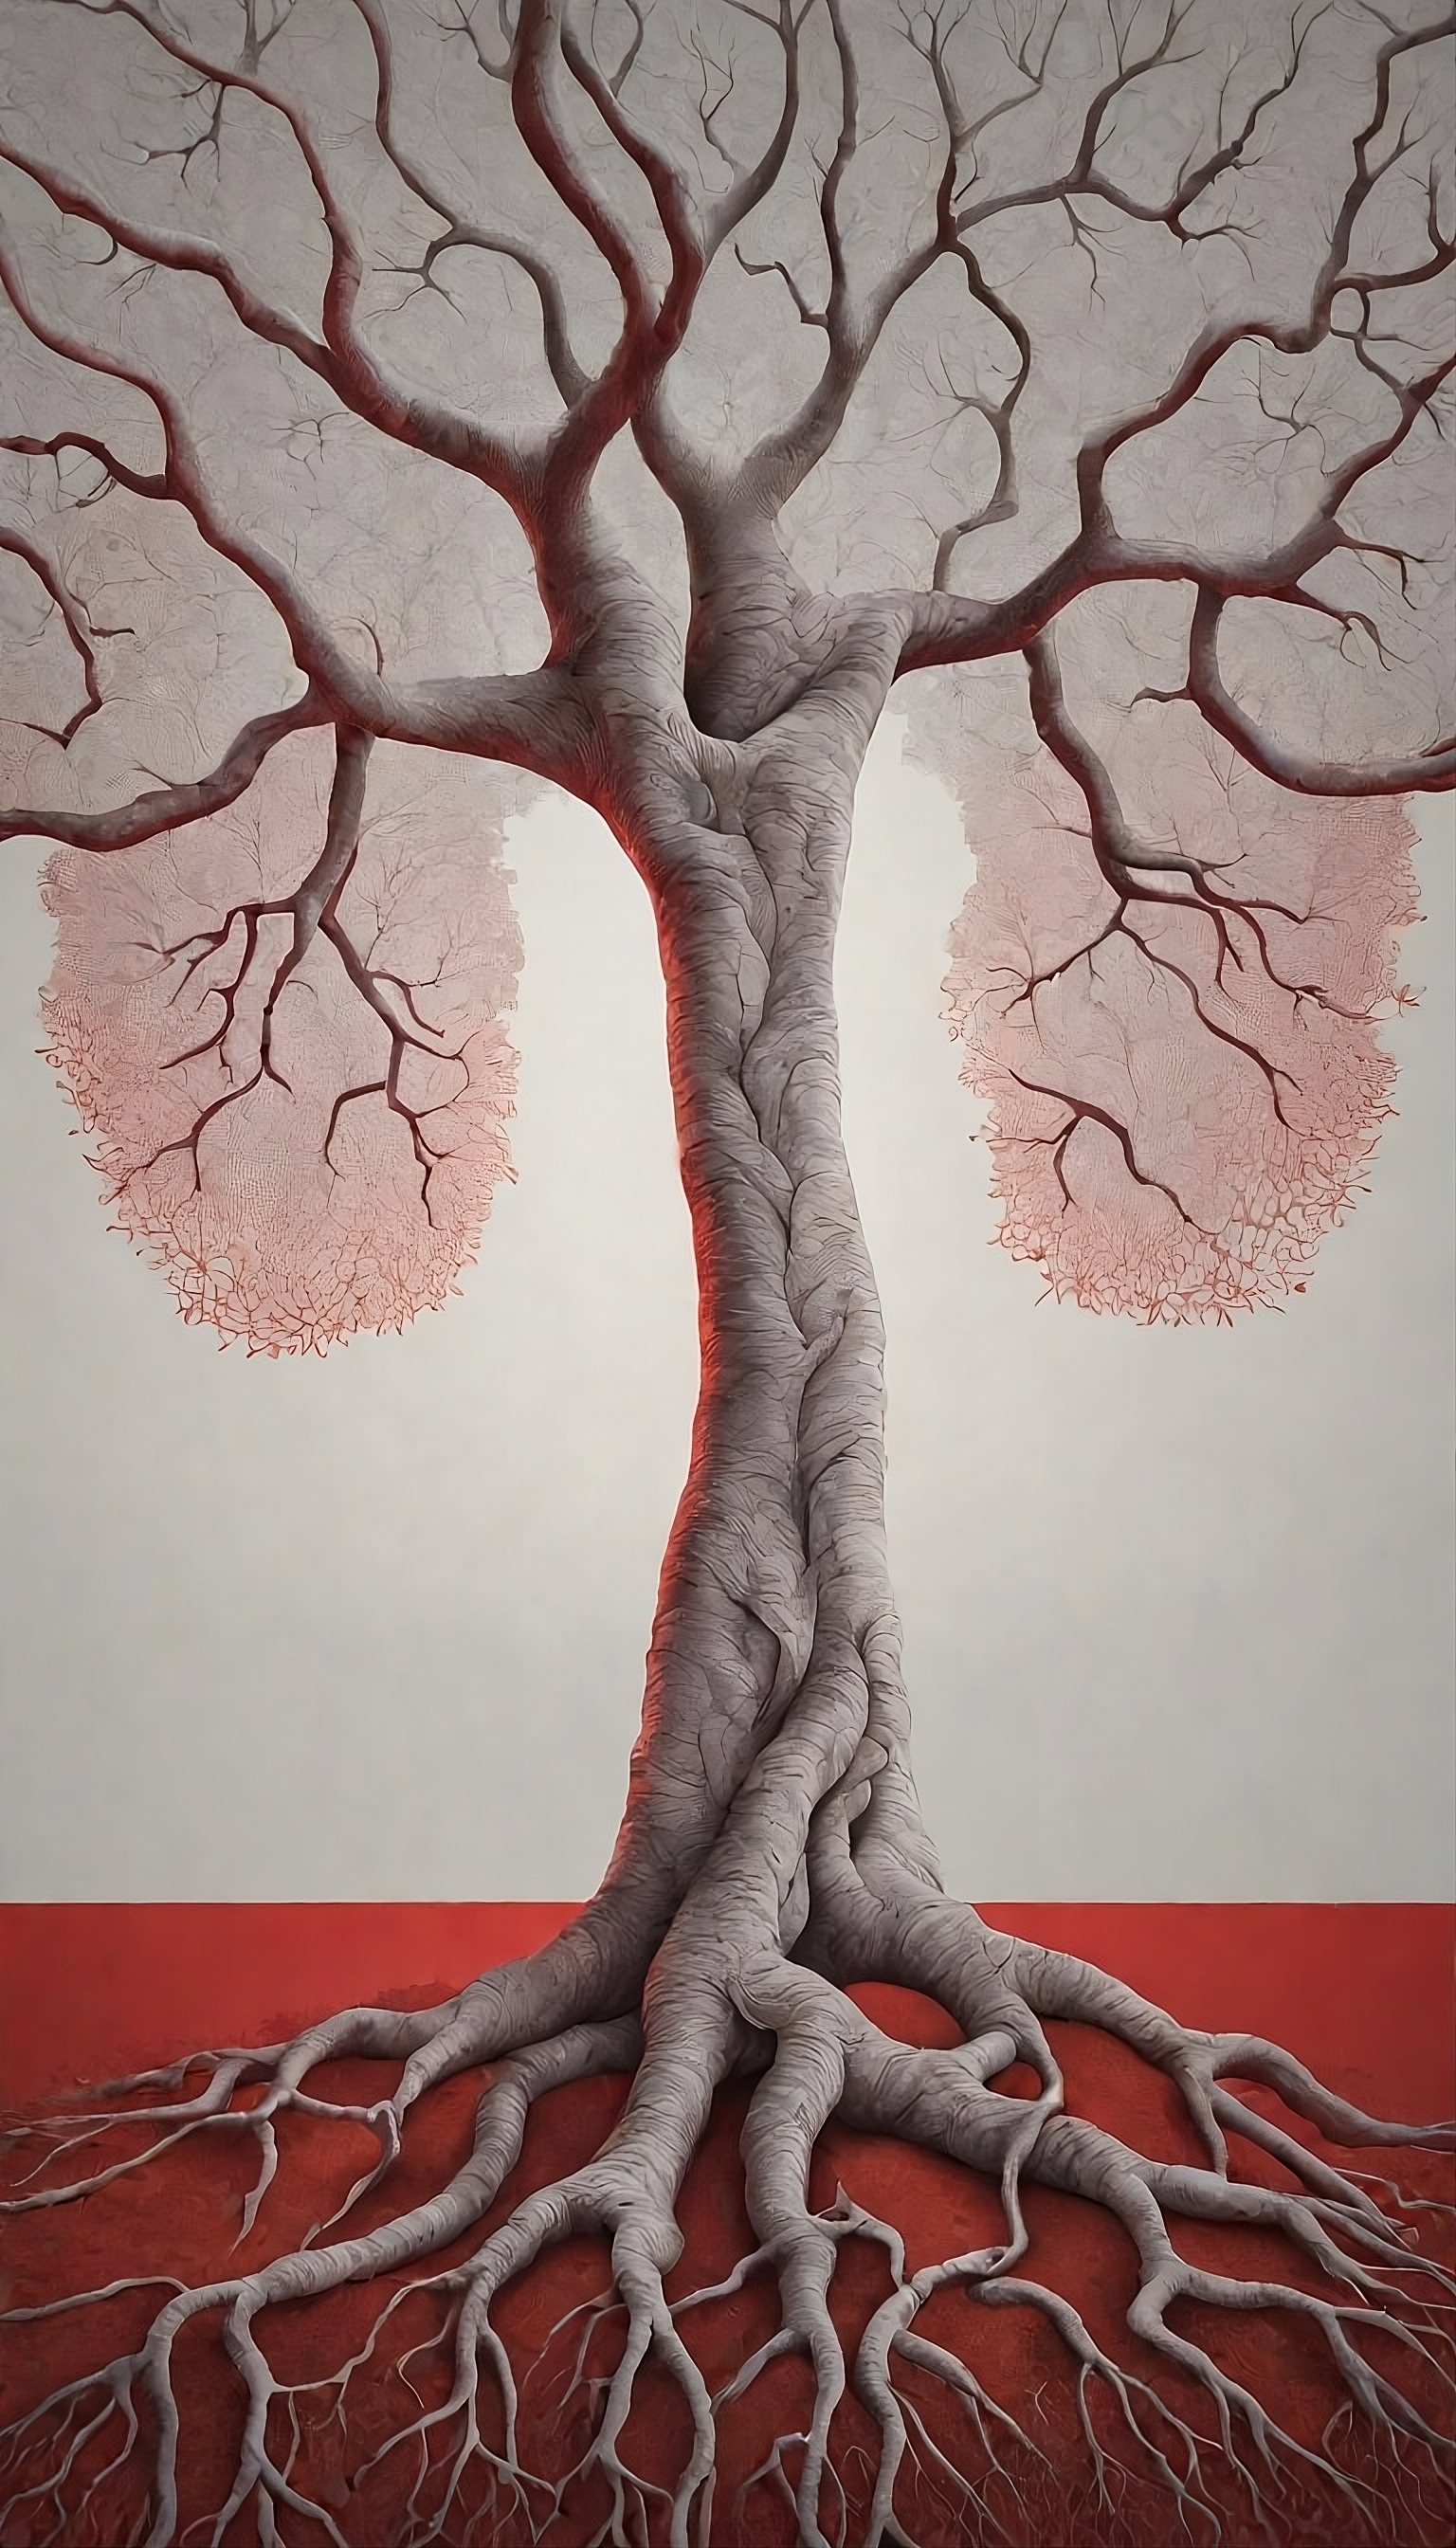
\includegraphics[width=\paperwidth,height=\paperheight]{resources/abstract-placenta-vignette_runwayml_upscaled.png}};
        \node[anchor = north west] at (current page.north west) {\includegraphics[scale=0.8]{resources/uon-logo-white.png}};
        \node [draw = white, line width = 2.5, align=center, inner sep=15pt, fill=black, fill opacity=.5, text opacity=1, shape=rectangle, minimum width=7cm, minimum height=3cm, anchor=center] at ($(current page.center) + (0,6cm)$) {\textcolor{white}{\LARGE\textbf{\textsf{\reporttitle}}} \\[14pt] \textcolor{white}{\Large\textbf{\textsf{{A computational study of maternal blood flow and}}}} \\ \textcolor{white}{\Large\textbf{\textsf{{oxygen transport in the human placenta}}}} \\[40pt] \textcolor{white}{\Large\textbf{\textsf{\reportauthor}}}};
        \node[anchor = south east] at ($(current page.south east) + (-1cm,0.5cm)$) {\textcolor{white}{\footnotesize\textsf{Image generated by \href{https://runwayml.com/}{Runway}}}};
    \end{tikzpicture}
    }%
}
\begin{titlepage}
    \setcounter{page}{1}
    \BgThispage
    \newgeometry{left=1cm,right=6cm,bottom=1.5cm}
    \vspace*{0.5\textheight}
    \noindent
    \vspace*{2cm}\par
    \noindent
    \vfill %ADDITION for when only name, not supervisors
    \begin{minipage}{0.35\linewidth}
        \begin{flushleft}
            % \printauthor
        \end{flushleft}
    \end{minipage} %\hspace{10pt}
\end{titlepage}
\restoregeometry

% Text-only title page.
\begin{titlepage}
    \setcounter{page}{2}
    \centering{
        \vspace*{1in}
        {   
            \textbf{\LARGE{\reporttitle}\\[6pt] \Large {\textsl{ {\reportsubtitle}}}}
        }
        \vskip 0.3in \par
        \large {\textbf{\reportauthorfull\;\textit{\reportauthortitles}}}
        \vfill
        \normalsize {Thesis submitted to the University of Nottingham\\for the degree of Doctor of Philosophy}
        \vskip 0.1in \par
        \normalsize{\bf{\reportdate}}
        \vskip 0.3in \par
        \Large {\textbf{Supervised by:}} \par
        \normalsize
        {
            \vskip 0.1in \par
            \textbf{Paul Houston} \vspace{3pt} \\
            \textbf{Matthew E Hubbard} \vspace{3pt} \\
            \textbf{Reuben D O'Dea}\\School of Mathematical Sciences\\University of Nottingham
        }
        % \vskip 0.3in \par
        % \Large {\textbf{Assessed by:}} \par
        % \normalsize
        % {
        %     \textbf{Matthew Scase}\\School of Mathematical Sciences\\University of Nottingham\vspace{7pt}\\
        %     \textbf{XXX}\\XXX\\XXX%
        % }
        % \vskip 0.3in \par
        % \normalsize {I hereby declare that this dissertation is all my own work, except as indicated in the text.}
        % \vskip 0.4in
        % \normalsize {Signature \underline{\hspace{1.5in}}}
        % \vskip 0.1in
        % \normalsize {Date \underline{\hspace{0.25in}} / \underline{\hspace{0.25in}} / \underline{\hspace{0.5in}}}
        % \vskip 0.4in \par
        % \normalsize {I hereby declare that I have all necessary rights and consents to publicly distribute this dissertation via the University of Nottingham's e-dissertation archive.}
    }
\end{titlepage}

    \todoitemthree{If printing: change to CYMK, ad blank pages, and add margins.}

    \pagenumbering{roman}
    \chapter*{Abstract}
        In this thesis, we present mathematical models used to describe maternal blood flow and oxygen transport in the at-term human placenta. We take a computational approach using discontinuous Galerkin finite element methods, which allows us to expand upon previous work by considering a complex 2D placental geometry that respects the main structural features of the placenta.
        
        One third of stillbirths are related to placental dysfunction, and therefore the overarching motivation for this work is to better understand characteristics of diseased placentas. This thesis studies maternal placental flow in three contexts, listed as follows.

        Firstly, we study how placental efficiency is affected by changes in structural parameters. We achieve this by generating a large number of flow and oxygen realisations, whereby parameters such as the number and position of arteries and veins in our computational domain are varied; this allows us to infer how changes in placental structure affect placental function.

        Taking the work in a second direction, we provide a method for comparing simulated flows with MRI data. We achieve this by advecting particles due to an underlying flow field, and modelling the evolution of each particle's magnetic spin, from which we can compute MRI signals. We compute these signals on simulated flow fields from our model of maternal blood flow, and on simpler manufactured sub-voxel shear flow, rotational flow, and accelerating flow fields; this allows us to infer the relationship between simple sub-voxel flow fields, our model of maternal blood flow, and real placental MRI data.

        Thirdly, we introduce a preliminary model of the recently-documented utero-placental pump, where the entire placenta periodically reduces by up to $40\%$ in volume, resulting in periodic ejection of blood from the placenta. We achieve this by prescribing a simple form of boundary motion in order to study the effect this has on flow and oxygen concentration. We show that contractions of this nature do influence the oxygen transport dynamics, and therefore could prove useful in understanding disease in the placenta.

    \chapter*{Acknowledgements}
        First and foremost, I am extremely grateful for the guidance and support of my supervisors. To Reuben O'Dea, thank you for your unwavering patience and encouragement, especially during the write-up process. To Matthew Hubbard, thank you for your keen eye on the details of several aspects of this project, and for bridging the mathematical gap between the biological and computational worlds. Finally, to Paul Houston, thank you for introducing me to finite elements and indeed this project, as well as the numerous hours you have spent helping me debug my terrible Fortran code.

        A special thank you to Penny Gowland and George Hutchinson for the many interactions on MRI matters, to Lopa Leach and Dimitrios Amanitis for everything biological, and to Zak Crowson for our many mathematical discussions. I would also like to acknowledge EPSRC for providing the funding for this project.

        I am also thankful to all those who have given me such an enjoyable 8 years in Nottingham. Thank you to those I've met through various academic encounters with reading groups, conferences, teaching, student rep work, and much-needed regular coffee breaks. I extend this thanks to those who I have met through extracurricular activities, including many orchestras and several organisations within Scouting; these hobbies have at times been the only things that have kept me sane.

        I am deeply indebted to the support of my family and friends, especially to my mam and late father, who provided an immense amount of encouragement throughout the first 18 years of my life, which prepared me for the life I have built in Nottingham, and have always supported me on whatever path I have chosen to take.

        I could not have completed this thesis without my partner, Eleanor, who has helped me maintain a work-life balance, tolerated my grumpiness, and nevertheless supported me through the inevitable highs and lows of a PhD. It remains for me to thank my dog, Pip, for brightening each day.

    \renewcommand{\thesection}{\hspace{-6pt}}
    \chapter*{Publications}
        Two publications have arisen from the work of this thesis and are currently in preparation.

        \section*{Chapter 4}
            Some of the work in Chapter \ref{sec:nutrient-uptake} is also presented in the publication \cite{crowsonInvestigatingPlacentalHemodynamics2024}. Specifically, the supervisors of this thesis have had oversight over the publication, with the author of this thesis focussing on the 2D investigations, and Zak Crowson\footnote{\href{mailto:zak.crowson2@nottingham.ac.uk}{zak.crowson2@nottingham.ac.uk}} focussing on 3D investigations. The results presented in this thesis take the 2D investigations to explore them in greater detail.

            \begin{itemize}
                \item[\cite{crowsonInvestigatingPlacentalHemodynamics2024}] Zak Crowson, \textbf{Adam Blakey}, Paul Houston, Matthew Hubbard, Lopa Leach, and Reuben O'Dea. \say{Investigating Placental Hemodynamics: A Morphological Sensitivity Study}. Manuscript in preparation. 2024.
            \end{itemize}

        \section*{Chapter 5}
            Some of the work in Chapter \ref{sec:numerical-mri} is also presented in the publication \cite{hutchinsonEffectsMaternalFlow2024}. Specifically, the author and supervisors of this thesis contributed to the mathematical models and numerical experiments, whilst in vivo data were collected and analysed by George Hutchinson\footnote{\href{mailto:george.hutchinson1@nottingham.ac.uk}{george.hutchinson1@nottingham.ac.uk}} and Penny Gowland\footnote{\href{mailto:penny.gowland@nottingham.ac.uk}{penny.gowland@nottingham.ac.uk}}. The results presented in this thesis take the mathematical model and numerical experiments to explore them in greater detail.

            \begin{itemize}
                \item[\cite{hutchinsonEffectsMaternalFlow2024}] George Hutchinson, \textbf{Adam Blakey}, Nia Jones, Lopa Leach, Paul Houston, Matthew Hubbard, Reuben O'Dea, and Penny Gowland. \say{The Effects of Maternal Flow on Placental Diffusion Weighted MRI and IVIM Parameters}. Manuscript in preparation. 2024.
            \end{itemize}

    \renewcommand{\thesection}{\arabic{chapter}.\arabic{section}}
    
    \tableofcontents

    %\tikzexternalize[prefix=tikz-cache/] % Caching of Tikz figures.

    \chapter{Introduction} \label{sec:introduction}
    \pagenumbering{arabic}
    %\rfoot{\iffloatpage{}{\footnotesize \thepage\ of \pageref{LastPage}}}
    \rfoot{\footnotesize \thepage\ of \pageref{LastPage}}

    % Opening introductory 1/2/3 paragraphs to setup thesis.
    % Paragraph to ouline the rest of the chapter.

    % Use ideas from FGR and PE to motivate the thesis.

    % \lettrine[lines=3]{\color{UoNBlue1}T}{his}
    This thesis utilises a mathematical model of maternal blood flow and oxygen concentration in the at-term human placenta, using a physiologically-informed 2D organ-scale geometry. The solutions are approximated using discontinuous Galerkin finite element methods from the existing numerical literature. The three main contributions of this thesis are to use the aforementioned model and numerics to investigate how placental structure influences flow and transport, to model MRI scans of flow, and to introduce a preliminary model of the newly-discovered utero-placental pump phenomenon.

    The remainder of this chapter presents a literature review of placental physiology and existing placental mathematical modelling.

    % 1.1 Placental physiology
    \section{Placental physiology}
        % To cover: structure and function in detail (concentrating on aspects of most relevance to the thesis). Touch on biomechanics and potential importace.
        % Diseases, and link back to relevance in this thesis.

        % Overview of placenta
        The placenta is a crucial organ that is essential for our birth. It is unique in that it can be straightforwardly examined ex vivo after delivery, enabling, for example, convenient ex vivo perfusion experiments to investigate placental function \cite{lewisPlacentalPerfusionMathematical2020,nyeHumanPlacentalOxygenation2018}. The role of the placenta is detailed by \citeauthor{jensenBloodFlowTransport2019} in \cite{jensenBloodFlowTransport2019}. In summary, the placenta has two main purposes: facilitating the transport of oxygen and nutrients from the mother to the fetus, and transporting carbon dioxide and waste products from the fetus to the mother. In human placentas, fetal blood flows through villous trees that are submerged in maternal blood, which flows through the surrounding intervillous space (IVS). Fetal and maternal blood do not directly mix: exchange between fetal and maternal blood takes place through the large surface area of the villous tree.

        % What does a placenta look like? Function; size and weight; structure.
        A healthy delivered placenta is usually disk-like with a typical diameter of \qty{22}{\centi\meter}, thickness of \qty{2.5}{\centi\meter}, and weight of \qty{470}{\gram} at full-term \cite{benirschkePathologyHumanPlacenta2012}. However, the in vivo measurements conducted by \citeauthor{afrakhtehCorrelationPlacentalThickness2013} \cite{afrakhtehCorrelationPlacentalThickness2013} using ultrasound have reported a larger average thickness of approximately \qty{3.6}{\centi\meter}, the disparity arising due to leakage of maternal blood and a pressure drop in the IVS after delivery, resulting in a collapse of placental structure and decrease in placental volume \cite{lecarpentierComputationalFluidDynamic2016,afrakhtehCorrelationPlacentalThickness2013}. Structurally, the placenta comprises many smaller functional units, partially separated from one another by so-called \textit{septal walls} or \textit{septa}. Naming conventions for these functional units differ between authors, with common words often found in the literature being \textit{lobe}, \textit{lobule}, \textit{cotyledon}, and \textit{placentone} \cite{kaufmannPlacentalVascularizationBlood1988}. The largest unit is called a \textit{lobe}, of which there are approximately $4$--$6$, with each \textit{lobe} containing approximately $8$--$10$ \textit{lobules}. An average healthy placenta is expected to contain between $30$ and $60$ \textit{lobules} \cite{serovRoleMorphologyMathematical2016,benirschkePathologyHumanPlacenta2012,kaufmannPlacentalVascularizationBlood1988}. \textit{Lobes} are distinguished by taller surrounding septal walls compared to \textit{lobules}, with recent measurements of the smaller and taller wall heights to respectively be on average \qty{6.90}{\milli\meter} and \qty{14.07}{\milli\meter} \cite{AMANITIS2023e68}. \textit{Placentones} are idealised units that correspond to one \textit{lobule} containing one villous tree \cite{kaufmannPlacentalVascularizationBlood1988,jensenBloodFlowTransport2019}. Placentones in the interior of the placenta are generally accepted to be approximately \qty{40}{\milli\meter} in diameter \cite{chernyavskyMathematicalModelIntervillous2010,lecarpentierComputationalFluidDynamic2016}, with smaller placentones as small as \qty{10}{\milli\meter} in diameter at the placental margin \cite{benirschkePathologyHumanPlacenta2012}. Figure \ref{fig:placenta:lobules} highlights lobes and lobules on the maternal side of a delivered placenta (i.e., the basal plate). For consistency, for the remainder of this thesis we will employ the terminology \textit{placentones} to denote all functional units surrounded by septal walls of any height.

        % Structure and vessels.
        Figure \ref{fig:placenta:cartoon} shows the structure of the placenta, with the maternal blood supply entering and exiting at the bottom, and the fetal blood supply entering and exiting at the top. Spiral arteries are the name given to maternal arteries entering the placenta. Brosens wrote in 1988 \cite{kaufmannPlacentalVascularizationBlood1988} that they found most spiral arteries were found on the basal plate or in the lower third of a septal wall, and estimated a total of 120 arterial openings over the entire placenta; there has also been evidence of chorionic veins \cite{benirschkePathologyHumanPlacenta2012}, and $5$--$6$ larger muscular veins thought to encircle the placenta, providing additional drainage \cite{nanaevHumanPlacentaEncircled2000}. The exact number of arteries and veins in a placenta may significantly vary from placenta to placenta, with current literature suggesting there to be $30$--$150$ arteries and $50$--$200$ veins for the maternal blood \cite{benirschkePathologyHumanPlacenta2012,chernyavskyMathematicalModelIntervillous2010,burtonRheologicalPhysiologicalConsequences2009}. Whilst several studies have focussed on maternal arterial flow (e.g., \cite{burtonRheologicalPhysiologicalConsequences2009,jamesTrophoblastPlugsImpact2018,saghianAssociationPlacentalJets2017,collinsDevelopmentalChangesSpiral2012}), few studies have considered the venous drainage, despite this being critical to the circulation of maternal blood, and therefore delivery of oxygen and nutrients \cite{hutchinsonFirstVivoDemonstration2020}. Furthermore, the location of vessels is not well understood; \citeauthor{chernyavskyMathematicalModelIntervillous2010} \cite{chernyavskyMathematicalModelIntervillous2010} outline the three main hypotheses for vein locations: random; concentrated near the placental margins, and concentrated near the placental septa \cite{boydHumanPlacenta1970}.

        \begin{figure}
            \thisfloatpagestyle{empty}
            \centering
            \begin{subfigure}[b]{0.6\textwidth}
                \centering
                \includegraphics[width=\textwidth]{diagrams/real-placenta-pictures/placenta-lobules.png}
                \caption{}
                \label{fig:placenta:lobules}
            \end{subfigure}
            \hfill
            \begin{subfigure}[b]{\textwidth}
                \centering
                

\tikzset{every picture/.style={line width=0.75pt}} %set default line width to 0.75pt        
\resizebox{\textwidth}{!}{%
\begin{tikzpicture}[x=0.75pt,y=0.75pt,yscale=-1,xscale=1,font=\sffamily]
%uncomment if require: \path (0,435); %set diagram left start at 0, and has height of 435

%Image [id:dp612682770859811] 
\draw (251.86,178.3) node  {\includegraphics[width=399.29pt,height=225.45pt]{diagrams/placenta-geometry-diagrams/placenta-cartoon-2024.png}};
%Straight Lines [id:da3701239304155397] 
\draw [color={rgb, 255:red, 71; green, 153; blue, 84 }  ,draw opacity=1 ][line width=1.5]    (438,136.13) -- (69.29,136.13) ;
\draw [shift={(65.29,136.13)}, rotate = 360] [fill={rgb, 255:red, 71; green, 153; blue, 84 }  ,fill opacity=1 ][line width=0.08]  [draw opacity=0] (11.61,-5.58) -- (0,0) -- (11.61,5.58) -- cycle    ;
\draw [shift={(442,136.13)}, rotate = 180] [fill={rgb, 255:red, 71; green, 153; blue, 84 }  ,fill opacity=1 ][line width=0.08]  [draw opacity=0] (11.61,-5.58) -- (0,0) -- (11.61,5.58) -- cycle    ;
%Shape: Arc [id:dp7839630490555429] 
\draw  [draw opacity=0][line width=1.5]  (487.26,230.95) .. controls (487.54,232.37) and (487.68,233.81) .. (487.68,235.27) .. controls (487.68,274.09) and (385.83,305.56) .. (260.18,305.56) .. controls (134.53,305.56) and (32.67,274.09) .. (32.67,235.27) -- (260.18,235.27) -- cycle ; \draw [color={rgb, 255:red, 71; green, 153; blue, 84 }  ,draw opacity=1 ][line width=1.5]    (487.68,234.94) .. controls (487.68,235.05) and (487.68,235.16) .. (487.68,235.27) .. controls (487.68,274.09) and (385.83,305.56) .. (260.18,305.56) .. controls (138.3,305.56) and (38.81,275.95) .. (32.95,238.74) ; \draw [shift={(32.67,235.27)}, rotate = 84.01] [fill={rgb, 255:red, 71; green, 153; blue, 84 }  ,fill opacity=1 ][line width=0.08]  [draw opacity=0] (11.61,-5.58) -- (0,0) -- (11.61,5.58) -- cycle    ; \draw [shift={(487.26,230.95)}, rotate = 94.26] [fill={rgb, 255:red, 71; green, 153; blue, 84 }  ,fill opacity=1 ][line width=0.08]  [draw opacity=0] (11.61,-5.58) -- (0,0) -- (11.61,5.58) -- cycle    ;
%Straight Lines [id:da8876380274555917] 
\draw [line width=1.5]    (181.85,82.47) -- (251.5,82.47) ;
\draw [shift={(255.5,82.47)}, rotate = 180] [fill={rgb, 255:red, 0; green, 0; blue, 0 }  ][line width=0.08]  [draw opacity=0] (11.61,-5.58) -- (0,0) -- (11.61,5.58) -- cycle    ;
%Straight Lines [id:da3261920772723992] 
\draw [line width=1.5]    (386,97.81) -- (334.04,185.37) ;
\draw [shift={(332,188.81)}, rotate = 300.69] [fill={rgb, 255:red, 0; green, 0; blue, 0 }  ][line width=0.08]  [draw opacity=0] (11.61,-5.58) -- (0,0) -- (11.61,5.58) -- cycle    ;
%Straight Lines [id:da23004860167795904] 
\draw [color={rgb, 255:red, 124; green, 71; blue, 153 }  ,draw opacity=1 ][line width=1.5]    (421,310.31) -- (376.68,240.74) ;
\draw [shift={(374.53,237.37)}, rotate = 57.5] [fill={rgb, 255:red, 124; green, 71; blue, 153 }  ,fill opacity=1 ][line width=0.08]  [draw opacity=0] (11.61,-5.58) -- (0,0) -- (11.61,5.58) -- cycle    ;
%Straight Lines [id:da26234807553589] 
\draw [color={rgb, 255:red, 218; green, 75; blue, 87 }  ,draw opacity=1 ][line width=1.5]    (260.68,314.42) -- (260.68,290.32) ;
\draw [shift={(260.68,286.32)}, rotate = 90] [fill={rgb, 255:red, 218; green, 75; blue, 87 }  ,fill opacity=1 ][line width=0.08]  [draw opacity=0] (11.61,-5.58) -- (0,0) -- (11.61,5.58) -- cycle    ;
%Straight Lines [id:da659245707576972] 
\draw [color={rgb, 255:red, 71; green, 85; blue, 153 }  ,draw opacity=1 ][line width=1.5]    (353.5,344.31) -- (326.23,255.23) ;
\draw [shift={(325.05,251.4)}, rotate = 72.98] [fill={rgb, 255:red, 71; green, 85; blue, 153 }  ,fill opacity=1 ][line width=0.08]  [draw opacity=0] (11.61,-5.58) -- (0,0) -- (11.61,5.58) -- cycle    ;
%Straight Lines [id:da0549441454891868] 
\draw [color={rgb, 255:red, 248; green, 140; blue, 147 }  ,draw opacity=1 ][line width=1.5]    (177,344.81) -- (195.28,263.52) ;
\draw [shift={(196.15,259.62)}, rotate = 102.67] [fill={rgb, 255:red, 248; green, 140; blue, 147 }  ,fill opacity=1 ][line width=0.08]  [draw opacity=0] (11.61,-5.58) -- (0,0) -- (11.61,5.58) -- cycle    ;
%Straight Lines [id:da750105190473205] 
\draw [color={rgb, 255:red, 71; green, 85; blue, 153 }  ,draw opacity=1 ][line width=1.5]    (454,121.81) -- (466.77,161.26) ;
\draw [shift={(468,165.06)}, rotate = 252.06] [fill={rgb, 255:red, 71; green, 85; blue, 153 }  ,fill opacity=1 ][line width=0.08]  [draw opacity=0] (11.61,-5.58) -- (0,0) -- (11.61,5.58) -- cycle    ;
%Image [id:dp6947304444659705] 
\draw (285.83,93.75) node  {\includegraphics[width=61.5pt,height=98.99pt]{diagrams/placenta-geometry-diagrams/placenta-cartoon-2024_uc.png}};
%Straight Lines [id:da1217993864688609] 
\draw [color={rgb, 255:red, 71; green, 85; blue, 153 }  ,draw opacity=1 ][line width=1.5]    (113.55,313.31) -- (113.55,262.4) ;
\draw [shift={(113.55,258.4)}, rotate = 90] [fill={rgb, 255:red, 71; green, 85; blue, 153 }  ,fill opacity=1 ][line width=0.08]  [draw opacity=0] (11.61,-5.58) -- (0,0) -- (11.61,5.58) -- cycle    ;

% Text Node
\draw (180.89,82) node [anchor=east] [inner sep=0.75pt]   [align=left] {Umbilical cord};
% Text Node
\draw (167.71,128.99) node [anchor=south] [inner sep=0.75pt]  [color={rgb, 255:red, 71; green, 153; blue, 84 }  ,opacity=1 ] [align=left] {Chorionic plate};
% Text Node
\draw (386,94.81) node [anchor=south] [inner sep=0.75pt]   [align=left] {Intervillous space (IVS)};
% Text Node
\draw (421,313.31) node [anchor=north] [inner sep=0.75pt]  [color={rgb, 255:red, 124; green, 71; blue, 153 }  ,opacity=1 ] [align=left] {Villous tree};
% Text Node
\draw (260.68,316.83) node [anchor=north] [inner sep=0.75pt]  [color={rgb, 255:red, 218; green, 75; blue, 87 }  ,opacity=1 ] [align=left] {Spiral artery};
% Text Node
\draw (64.67,279.61) node [anchor=north] [inner sep=0.75pt]  [color={rgb, 255:red, 71; green, 153; blue, 84 }  ,opacity=1 ,rotate=-24.27] [align=left] {Basal plate};
% Text Node
\draw (177,347.81) node [anchor=north] [inner sep=0.75pt]  [color={rgb, 255:red, 248; green, 140; blue, 147 }  ,opacity=1 ] [align=left] {Septal wall};
% Text Node
\draw (454,118.81) node [anchor=south] [inner sep=0.75pt]  [color={rgb, 255:red, 71; green, 85; blue, 153 }  ,opacity=1 ] [align=left] {Marginal sinus vein};
% Text Node
\draw (353.5,347.31) node [anchor=north] [inner sep=0.75pt]  [color={rgb, 255:red, 71; green, 85; blue, 153 }  ,opacity=1 ] [align=left] {Septal wall vein};
% Text Node
\draw (113.55,316.31) node [anchor=north] [inner sep=0.75pt]  [color={rgb, 255:red, 71; green, 85; blue, 153 }  ,opacity=1 ] [align=left] {Basal plate vein};



\end{tikzpicture}
}
                \caption{}
                \label{fig:placenta:cartoon}
            \end{subfigure}
            \caption{(a) Annotated picture provided via private communications with Lopa Leach\protect\footnote{\href{mailto:lopa.leach@nottingham.ac.uk}{lopa.leach@nottingham.ac.uk}} and Dimitrios Amanitis\protect\footnote{\href{mailto:dimitrios.amanitis1@nottingham.ac.uk}{dimitrios.amanitis1@nottingham.ac.uk}}. Picture of the basal plate of a human placenta, with grooves showing visible septal walls. Coloured lines segment the placenta into 5 lobes, with white `L's indicating locations of individual lobules. (b) Modified diagram from \cite{dellschaftHaemodynamicsHumanPlacenta2020}, showing how blood moves through the placenta. The chorionic plate is shown towards the top of the picture, and the basal plate is at the bottom. Septal walls separate individual placentones. Maternal blood enters the placenta via the spiral arteries before percolating through the IVS and exiting through one of three types of vein: basal plate, septal wall, or marginal sinus. Fetal blood enters via the umbilical cord, flows through fetal vessels that cross the chorionic plate, before flowing through the villous trees, and finally returning to the umbilical cord.}
            \label{fig:placenta}
        \end{figure}

        % Development of the placenta throughout gestation.
        The placenta is an organ that develops through gestation, undergoing many structural changes from its initial development to delivery \cite{clarkComputationalModelingInteractions2021}, which complicates placental study. For example, ultrasound measurements indicate placental thickness measured from the umbilical cord insertion site increases almost three-fold between the first and third trimesters (first 14 weeks and after 27 weeks of pregnancy, respectively), increasing from \qty{12.90}{\milli\metre} to \qty{34.67}{\milli\metre} \cite{banikPlacentalThicknessMeasurement2022}. As well as the placenta overall increasing in size, other structural components separately undergo changes. For example, so-called `trophoblast plugs' are present only from approximately 5 weeks of gestation, where cells partially block the spiral artery and promote remodelling (widening) \cite{jamesTrophoblastPlugsImpact2018}. Another example is the villous tree, which matures during gestation to become more specialised for diffusional exchange \cite{hempstockIntralobularDifferencesAntioxidant2003}. This thesis will consider only at-term placentas.

        % Villous tree.
        The exchange of several solutes, including oxygen, takes place through the villous tree, which has a huge surface area  --- approximately $\qty{10}{\metre^2}$, or roughly $10\%$ of the surface area of an adult human's lungs \cite{clarkComplexitiesHumanPlacenta2023}. Efficient exchange often requires maternal blood to access the whole of the villous tree (i.e., areas far from the basal plate), in order to maximise possible uptake area. Figure \ref{fig:hempstock2003} shows how blood enters through spiral arteries, moves through the central cavity (CC), percolates through increasingly mature villous tree material, and then finally exits through one of several veins --- including septal wall veins, marginal sinuses, and other veins located outside the originating placentone by passing over septal walls; naturally, the oxygen concentration in the blood reduces as it passes through the villous tree due to oxygen uptake. It has been postulated that villous density close to spiral arteries must decrease during gestation, in order to account for so-called `mega-jets' that permit deep penetration of nutrient-rich blood \cite{saghianAssociationPlacentalJets2017}. \citeauthor{hempstockIntralobularDifferencesAntioxidant2003} \cite{hempstockIntralobularDifferencesAntioxidant2003} explain that villi nearer to the central cavity are of a larger diameter, and are less specialised for diffusional exchange than their counterparts in the periphery; it is therefore advantageous for high oxygen concentration blood to reach peripheral villi.

        \begin{figure}
            \centering
            \includegraphics[width=0.6\textwidth]{diagrams/other-paper-figures/hempstock2003.png}
            \caption{Reproduced Figure from \cite{hempstockIntralobularDifferencesAntioxidant2003} showing a single placentone containing a villous tree. The triangles on the left show that outward from the central cavity there is an increasing maturation of villi and a decreasing concentration of blood oxygen.}
            \label{fig:hempstock2003}
        \end{figure}

        % Placental diseases.
        Nutrient delivery is essential for normal fetal growth, with poor delivery of nutrients often linked to pregnancy complications such as stillbirth. A complication of disease study is that some placental diseases are specific to humans \cite{clarkComplexitiesHumanPlacenta2023}, due to radical structural variations between mammalian placentas \cite{laundonPlacentalEvolutionThreedimensional2024}. Pre-eclampsia (PE), for example, is a complex, multisystem disease that is unique to humans, characterised by sudden-onset hypertension \cite{burtonRheologicalPhysiologicalConsequences2009,dimitriadisPreeclampsia2023}. Fetal growth restriction (FGR) is another placental disease that is often associated with stillbirth \cite{smithStillbirth2007}, and is defined as the failure of the fetus to achieve its genetically-determined growth potential \cite{resnikIntrauterineGrowthRestriction2002}, with FGR placentas on average half of the size of normal placentas \cite{sunPlacentaFetalGrowth2020}. PE and FGR are both generally considered to be associated with structural defects in the placenta, leading to impaired nutrient delivery and complications for both the fetus and mother, particularly when spiral arteries fail to widen upon entering the IVS \cite{burtonPathophysiologyPlacentalderivedFetal2018,dellschaftHaemodynamicsHumanPlacenta2020}. In healthy placentas, spiral arteries widen from \qty{0.5}{\milli\metre} to \qtyrange{2}{3}{\milli\metre}, allowing upstream flow to slow from $\qty{1}{\metre\per\second}$ to $\qty{0.1}{\metre\per\second}$; however, in diseased cases, the failure to widen can result in flow at $\qty{1}{\metre\per\second}$ to directly enter the placenta \cite{burtonRheologicalPhysiologicalConsequences2009}. Whilst an increase in flow speed encourages deeper penetration of blood, speeds that are too high will damage villous tree structures, creating an overall smaller uptake area, and reduce blood transit times such that blood leaves the placenta with higher-than-usual oxygen concentrations \cite{burtonRheologicalPhysiologicalConsequences2009}. Understanding which structural changes happen in disease, and the extent to which they impair blood flow and nutrient delivery, may ultimately prove crucial for clinicians looking to treat these diseases. Another source of nutrient delivery impairment has been suggested to be due to whether mothers choose to sleep on their back or on their side; \citeauthor{couperEffectsMaternalPosition2021} \cite{couperEffectsMaternalPosition2021} report that maternal flow rates lower by $27\%$ when mothers are on their backs, as well as a $11.2\%$ decrease in delivery of oxygen to the fetus. This phenomenon occurs even in healthy late-gestation pregnancies, which could be in part an explanation for late-gestation stillbirths. 

        % Speed of flow.
        The work of \citeauthor{burtonRheologicalPhysiologicalConsequences2009} \cite{burtonRheologicalPhysiologicalConsequences2009} and \citeauthor{rothDynamicModelingUteroplacental2017} \cite{rothDynamicModelingUteroplacental2017} focusses on the effects of high flow speed from spiral arteries and the association with diseases such as FGR and PE, and reported the presence of vortices and turbulence in areas surrounding the artery. Even in healthy pregnancies, the speed of flow in the placenta varies greatly from the basal plate to the sub-chorionic space (the region below the chorionic plate, see Figure \ref{fig:placenta:cartoon}). \citeauthor{dellschaftHaemodynamicsHumanPlacenta2020} \cite{dellschaftHaemodynamicsHumanPlacenta2020} gathered data on the speed in the placenta using MRI, and categorised regions of fast flow (flow faster than $\qty{1e-3}{\metre\per\second}$) and slow flow (flow slower than $\qty{5e-4}{\metre\per\second}$), finding that the faster regions were predominantly concentrated on the basal plate. Additionally, they found that there was a distinct difference in the average speed found in the IVS between healthy (\qty{4e-4}{\metre\per\second}) and diseased (\qty{7e-4}{\metre\per\second}) placentas \cite{dellschaftHaemodynamicsHumanPlacenta2020}. 

         % Different types of contractions.
        In addition to dynamics which could arise directly from maternal and fetal blood flow, there are several other forms of movement in the placenta, such as contractions of the villous tree or contractions of the entire uterus; several authors have documented the properties of such phenomena since as early as 1963 \cite{krantzContractilePropertiesSmooth1963,farleyContractilePropertiesHuman2004,lecarpentierUltraslowMyosinMolecular2014,togashiSustainedUterineContractions1993}. However, the newly documented `utero-placental pump' phenomenon is a contraction involving only the placenta \cite{dellschaftHaemodynamicsHumanPlacenta2020}. \citeauthor{dellschaftHaemodynamicsHumanPlacenta2020} \cite{dellschaftHaemodynamicsHumanPlacenta2020} report that it has been found experimentally that placental volume can reduce by up to 40\% in these `utero-placental pump' contractions over a 10-minute period, resulting in a periodic ejection of blood from the IVS. 

        % Perfusion experiments.
        Delivered placentas, whilst generally readily-available after birth, undergo significant structural changes outside the uterus \cite{lecarpentierComputationalFluidDynamic2016}, rendering ex vivo experiments of limited use. One way of overcoming the deflation issue is to perform perfusion experiments soon after delivery, where a placentone is identified in a freshly delivered placenta, and both the maternal and fetal blood supplies are catheterised \cite{schneiderModifiedDoublecircuitVitro1984,lewisPlacentalPerfusionMathematical2020}; these have then been coupled with mathematical models, giving a well-controlled system in which to test parameters and gain physiological understanding \cite{lewisPlacentalPerfusionMathematical2020}. In the case where placentas fail entirely, artificial placentas have been developed since as early as the 1950s with variable success; however, important progress towards the ultimate goal of a functioning artificial human placenta has been made through important contributions to placental research throughout the 2010s \cite{tunDifferencesPlacentalCapillary2019,saghianAssociationPlacentalJets2017,katoVillousTreeModel2017,serovOptimalVilliDensity2015,serovRoleMorphologyMathematical2016,lecarpentierComputationalFluidDynamic2016,clarkMultiscaleModellingFeto2015,chernyavskyTransportPlacentaHomogenizing2011,chernyavskyMathematicalModelIntervillous2010,burtonRheologicalPhysiologicalConsequences2009,lewisPlacentalPerfusionMathematical2020}.
        
        % Digital twins.
        Mathematical modelling is a powerful tool in developing understanding of behaviour in complex systems, such as the placenta and other organs. Digital twins are regarded as the gold standard of organ modelling, where simulations directly model a specific real-world organ. Sufficiently developed digital twins of the placenta would allow clinicians to study disease and the effects of medical intervention in a risk-free environment. Whilst there are currently no such models of the entire placenta, mathematical modelling of the heart has made use of patient-specific geometries \cite{taoDigitalTwinModeling2022}, with projects such as iHEART contributing to collective understanding of the organ \cite{zingaroComprehensiveMathematicalModel2023}. Upon the path leading to digital twins of the human placenta lies several issues that must first be tackled by the modelling community; \citeauthor{jensenBloodFlowTransport2019} \cite{jensenBloodFlowTransport2019} detail the important issues as modelling deformability of villous trees, impact from the external environment, 3D morphology at a statistical level, development of the placenta from early pregnancy, transport of multiple substances, and understanding structural variations across placental mammalian species.
        
    \section{Flow and transport in the placenta}
        % Fetal/maternal flow in isolation.
        Most current mathematical models consider either the fetal or maternal blood flow in isolation. This thesis focusses solely on modelling the maternal blood, but we now give a brief overview of fetal modelling approaches.

        % Fetal modelling.
        \citeauthor{zhangRecastingCurrentKnowledge2023} \cite{zhangRecastingCurrentKnowledge2023} highlight the importance of computational models in the study of fetal blood flow.
        The behaviour of fetal blood is often directly linked to the structure of the villous tree, leading many recent studies to use anatomical images to study fetal flow behaviour on the scale of individual villous tree `leaves' \cite{erlichPhysicalGeometricDeterminants2019,erlichQuantifyingImpactTissue2019,pearceImageBasedModelingBlood2016,plitmanmayoThreedimensionalModelingHuman2016}. \citeauthor{clarkMultiscaleModellingFeto2015} \cite{clarkMultiscaleModellingFeto2015} were instead able to create an anatomically based geometric model of the entire fetal villous tree, and used a simple flow model to study how fetal blood was affected by changes to the structure of the tree. The umbilical cord carries the fetal blood to and from the placenta; \citeauthor{kasiteropoulouComputationalFluidDynamics2020} \cite{kasiteropoulouComputationalFluidDynamics2020} studied the structure of the umbilical cord and how this impacts heat exchange, finding that the helicity of the cord plays a vital role in fetal thermoregulation.

        % Types of maternal modelling.
        In the existing literature, there are generally two approaches to modelling maternal blood flow \cite{jensenBloodFlowTransport2019}. Firstly, there are pore-scale (or micro-scale) models, where `pore' refers to the volume between villous tree branches; for example, \citeauthor{lecarpentierComputationalFluidDynamic2016} \cite{lecarpentierComputationalFluidDynamic2016} take 2D anatomical images of the villous trees and use the Navier-Stokes equations to model blood flow through the pores, although the method of imaging was not reported. An inherent issue with this 2D approach is that tree material can form impenetrable barriers in the plane, a constraint that 3D flow models may overcome. \citeauthor{serovOptimalVilliDensity2015} \cite{serovOptimalVilliDensity2015} used the micro-scale approach to simulate flow through a `stream-tube placenta model' and measured oxygen uptaken by the villous tree, ultimately finding an optimal villous density of approximately $0.47$ maximises oxygen uptake, which is consistent with previous experimental measurements. Secondly, there are tree-scale (or macro-scale) models, which model flow through gaps in the tree branches as a porous medium via, for example, a Darcy-type description \cite{lecarpentierComputationalFluidDynamic2016,chernyavskyMathematicalModelIntervillous2010,erianMaternalPlacentalBlood1977}; this involves creating a resistance to flow, which can be described by a permeability (equivalently hydraulic conductivity) $k$, for which the size of $k$ is inversely proportional to the effective flow resistance.

        % Majority of the Darcy-type maternal modelling.
        In \citeyear{erianMaternalPlacentalBlood1977}, \citeauthor{erianMaternalPlacentalBlood1977} \cite{erianMaternalPlacentalBlood1977} were the first to model maternal placenta flow computationally. They modelled the placentone as a square, through which blood flowed according to Darcy's law, with a permeability field that varied with position, accounting in a simple way for a less-permeable central cavity region. This porous medium approach has been adopted more recently by \citeauthor{chernyavskyMathematicalModelIntervillous2010} \cite{chernyavskyMathematicalModelIntervillous2010} where they derive analytical expressions for the blood flow field, under the assumption of Darcy flow in a 3D hemispherical domain representing a single placentone. \citeauthor{lecarpentierComputationalFluidDynamic2016} \cite{lecarpentierComputationalFluidDynamic2016} computationally modelled flow through a single 2D placentone, from which they were able to inform wall shear stress (WSS) villous tree measurements on several small areas cut out from the domain. This work provides valuable insight into the stresses experienced by cells in the villous tree, as it is believed that diseases such as PE may be attributed to damage to the villous tree caused by high-speed flow \cite{burtonRheologicalPhysiologicalConsequences2009}.

        % Central cavity.
        The central cavity is a villous-free region above the spiral artery mouth, thought to form among the villous tree material due to stresses from incoming maternal blood flow \cite{burtonRheologicalPhysiologicalConsequences2009,saghianAssociationPlacentalJets2017}. This region provides a lower resistance to flow, allowing incoming high-speed flow to penetrate deeper into the placenta before entering the IVS. In the context of the placenta, regions of high-speed flow (faster than $\qty{0.1}{\metre\per\second}$) are referred to as `jets' \cite{saghianAssociationPlacentalJets2017}. Ultrasound imaging have found so-called `mega-jets', which are jets longer than half of the placental thickness, and are components of a normal pregnancy \cite{collinsDevelopmentalChangesSpiral2012}. \citeauthor{saghianAssociationPlacentalJets2017} \cite{saghianAssociationPlacentalJets2017} modelled flow entering the IVS throughout gestation, finding that the presence of mega-jets requires regions of less dense villous tree, such as the central cavity. 
        
        % Advancements.
        Some authors employ a hybrid between the micro- and macro-scale approaches, using micro-scale simulations to determine values of local permeability, which then informs the macro-scale dynamics through a spatially varying permeability field \cite{lecarpentierComputationalFluidDynamic2016,linMultiscaleModelPlacental2016}. Some authors who use macro-scale models make further modelling enhancements such as varying the permeability throughout the domain \cite{lecarpentierComputationalFluidDynamic2016,erianMaternalPlacentalBlood1977}, or modelling the effect of artery widening before the maternal blood enters the IVS, to study what effect this has on fetal development \cite{burtonRheologicalPhysiologicalConsequences2009,rothDynamicModelingUteroplacental2017,saghianAssociationPlacentalJets2017}. Whilst most of the mathematical placental literature studies third trimester placentas (usually regarded as `fully developed' or `at term'), some authors have investigated the placenta throughout its development. For example, \citeauthor{jamesTrophoblastPlugsImpact2018} \cite{jamesTrophoblastPlugsImpact2018} computationally investigated the effect of trophoblast plugs, with their work suggesting that trophoblast plugs play an important role in rate-limiting flow to the placenta, and that malformation of these plugs can lead to diseased placentas. Little is known about the rheology of blood in the IVS when compared to blood rheology in narrow capillaries, which have been well-characterised experimentally, and instead authors model maternal blood flow in the IVS as incompressible \cite{chernyavskyMathematicalModelIntervillous2010}.

        % Transport models.
        Exchange from mother to fetus is also an important aspect to study, for which the flow of blood can be regarded as a vehicle in which to transport oxygen, nutrients, and waste products. Some authors have modelled transport using a reaction-advection equation for oxygen or nutrient concentration \cite{perazzoloModellingEffectIntervillous2017,perazzoloModellingNutrientTransfer2016,chernyavskyMathematicalModelIntervillous2010}, whilst others have supplemented the reaction-advection equation using Henry's law, which additionally describes enhancement to advection due to oxygen's affinity for haemoglobin \cite{serovOptimalVilliDensity2015,erlichPhysicalGeometricDeterminants2019,pearceImageBasedModelingBlood2016,meklerImpactTissuePorosity2022,serovOptimalVilliDensity2015,pearceImageBasedModelingBlood2016}.

        % Contractions.
        Given that the placenta lacks stiff supporting inner structures, a poroelastic description is likely appropriate \cite{jensenBloodFlowTransport2019}. Moreover, throughout gestation, contractions of the placenta and surrounding uterus have been widely reported \cite{dellschaftHaemodynamicsHumanPlacenta2020,togashiSustainedUterineContractions1993,farleyContractilePropertiesHuman2004}. However, as far as we are aware, there is currently only one paper that presents a mathematical model that describes contractions. \citeauthor{katoVillousTreeModel2017} \cite{katoVillousTreeModel2017} focussed on the effect of actively contracting villous trees, finding the contractions to be useful for both the fetal and maternal blood circulations due to resulting displacements. Whilst the recently-discovered utero-placental pump is yet to be mathematically modelled, it is thought that these contractions may be related to the previous reports of contracting villous trees \cite{dellschaftHaemodynamicsHumanPlacenta2020}.

        % Coupled models.
        Little work has been undertaken on fully-coupled transport models describing both maternal and fetal flow simultaneously, especially at the organ-scale. The first coupled transport paper we are aware of is from 1973, where \citeauthor{hillMathematicalModelCarbon1973} \cite{hillMathematicalModelCarbon1973} used a simple compartmental model to describe the transport of oxygen and carbon dioxide between maternal and fetal blood, which allowed the authors to investigate the relationship between Haldane and Bohr effects and transport. More recently, the use of mathematical models in combination with perfusion experiments is summarised by \citeauthor{lewisPlacentalPerfusionMathematical2020} \cite{lewisPlacentalPerfusionMathematical2020}, where the authors highlight several studies that have used compartmental models --- which describes how solutes may pass between mother, placenta, and fetus --- in order to study the bidirectional transport behaviour of various solutes in artificial perfusion experiments \cite{stirratTransferMetabolismCortisol2018,perazzoloInfluencePlacentalMetabolism2017,lofthouseComputationalModellingParacellular2023,hirschmuglPlacentalMobilizationFree2021}. Other related studies have modelled solute passing from maternal flow to the fetal capillaries, but for simplicity neglect the fetal flow itself \cite{perazzoloModellingEffectIntervillous2017}.

        % Structural variations.
        One of the most significant difficulties of placental study is that structural variability is not well understood \cite{jensenBloodFlowTransport2019}. To illustrate this, \citeauthor{benirschkePathologyHumanPlacenta2012} \cite{benirschkePathologyHumanPlacenta2012} took two vastly different estimates of the number of spiral arteries from previous studies, where one author estimated $263$, whilst another estimated just $25$; the disparity here is likely due to difficulties in identifying the arteries, and also due to functional changes to the arteries during development \cite{benirschkePathologyHumanPlacenta2012}. Contrasting estimates can also be found for other structural features, such as the number and position of veins \cite{chernyavskyMathematicalModelIntervillous2010,boydHumanPlacenta1970}, and the number of placentones \cite{benirschkePathologyHumanPlacenta2012,kaufmannPlacentalVascularizationBlood1988,serovOptimalVilliDensity2015,boydHumanPlacenta1970}. In the absence of a concrete understanding of many important structural features, several studies have used mathematical models to investigate their impact on placental behaviour. For example, \citeauthor{chernyavskyMathematicalModelIntervillous2010} \cite{chernyavskyMathematicalModelIntervillous2010}, and more recently \citeauthor{meklerImpactTissuePorosity2022} \cite{meklerImpactTissuePorosity2022}, studied how vein placement affects oxygen uptake to the villous tree; they found that veins too close to the artery would exhibit `short-circuiting' behaviour, where flow is very much localised to the region between the arteries and veins, thus limiting oxygen uptake. \citeauthor{chernyavskyMathematicalModelIntervillous2010} \cite{chernyavskyMathematicalModelIntervillous2010} also studied how the height of the villous-free central cavity influences oxygen concentration, finding deeper penetration of oxygen for larger cavity sizes.

        % Standard maternal blood flow model.
        A standard model in the maternal mathematical literature has been to allocate one artery and two veins on the basal plate to a placentone, with mathematical models of maternal blood flow restricted to placentones, and therefore do not consider either septal wall or marginal sinus veins. This is a clear limitation of existing studies as flux of blood between neighbouring placentones, as would be expected in the sub-chorionic space (SCS) \cite{jensenBloodFlowTransport2019}, is necessarily neglected. Furthermore, additional drainage due to septal wall veins and marginal sinus veins have not been considered in flow models, despite reports of their existence in the literature \cite{hempstockIntralobularDifferencesAntioxidant2003,AMANITIS2023e68,nanaevHumanPlacentaEncircled2000}. Although there are several works related to simulations of entire fetal villous trees (e.g., \cite{clarkMultiscaleModellingFeto2015,tunDifferencesPlacentalCapillary2019}), as far as we are aware, there is not any published work that tackles simulations of maternal blood flow on the scale of the entire placenta.
        
        % What we're doing.
        In this thesis, we exclusively use a macro-scale model of maternal blood flow. This approach eliminates the need for fine villous tree meshes, gives the permeability field as a simple function of the spatial coordinates, and avoids challenges that arise with impermeable villous tree structures in 2D. We will also adopt some of the modelling enhancements in the aforementioned references, such as the inclusion of a central cavity and a widening spiral artery. As noted by \citeauthor{jensenBloodFlowTransport2019} in \cite{jensenBloodFlowTransport2019}, the described approaches for maternal haemodynamics are mostly restricted to single placentones; \citeauthor{jensenBloodFlowTransport2019} further note that there is meaningful progress still to be made at the whole-organ level, and with validating models against experimental data. We will therefore solve a macro-scale model on a representative 2D slice of a whole placenta, which as far as we are aware, is a novel contribution of this thesis. This 2D geometry is simpler than an equivalent 3D geometry, but captures the main structural features of the placenta. Our blood flow model will be supplemented with a model of oxygen transport so that we may study oxygen uptake by the fetal villous tree. The thesis will then develop in three separate settings: to investigate how placental structure influences flow and transport; to model MRI scans of placental flow; and to introduce a preliminary model of utero-placental pump.
        
    \section{Models of flow} 
        % Darcy's law.
        Poromechanics more generally describes the behaviour of fluids saturating porous media, where the fluid may be a liquid or a gas, and the structure is often permeable or elastic (e.g., \cite{collisEffectiveEquationsGoverning2017}). The simplest example of steady flow through a porous medium is Darcy's law. For a bounded domain $\Omega \subset \RR^d$, for $d = 2, 3$, Darcy's law is given by
        \begin{equation}
            \frac{\mu}{k} \vec{u} + \vec{\nabla}p = 0,
            \label{eq:darcy-law}
        \end{equation}
        where $\vec{u}$ is the vector velocity field of the fluid, $p$ is the scalar pressure field, $k$ is permeability, and $\mu$ is the dynamic viscosity of the fluid. We have omitted boundary conditions here for ease of presentation.

        % Navier-Stokes.
        The Navier-Stokes equations model time-dependent, viscous, Newtonian (non-porous) fluid flow. The incompressible Navier-Stokes equations are given as: find $\vec{u}, p$ such that
        \begin{subequations}
            \begin{align}
                \begin{split}
                    \rho \pdv{\vec{u}}{t} + \rho (\vec{u} \cdot \vec{\nabla}) \vec{u} - \mu \nabla^2 \vec{u} + \vec{\nabla} p & = \rho \vec{f},
                \end{split}\\
                \begin{split}
                    \vec{\nabla} \cdot \vec{u} & = 0,
                \end{split}%
            \end{align}%
            \label{eq:navier-stokes}%
        \end{subequations}%
        where $\rho$ is the density of the fluid, and $\vec{f}$ is some body force acting on the fluid. One may define the Reynolds number as $\Rey := \frac{\rho U L}{\mu}$, for some appropriate choices of velocity and length scalings ($U$ and $L$, respectively), which describes the ratio between inertial and viscous forces. By assuming that the inertial forces are small compared to viscous forces, the Reynolds number is low (i.e., $\Rey \ll 1$), Equation \eqref{eq:navier-stokes} at leading order reduces to Stokes flow: find $\vec{u}, p$ such that
        \begin{subequations}
            \begin{align}
                \begin{split}
                    - \mu \nabla^2 \vec{u} + \vec{\nabla} p & = \vec{f},
                \end{split}\\
                \begin{split}
                    \vec{\nabla} \cdot \vec{u} & = 0.
                \end{split}
            \end{align}
            \label{eq:stokes-flow}
        \end{subequations}
        
        % Brinkman.
        In \citeyear{brinkmanCalculationViscousForce1949}, \citeauthor{brinkmanCalculationViscousForce1949} \cite{brinkmanCalculationViscousForce1949} introduced a modification of Darcy's law in Equation \eqref{eq:darcy-law}, which we will refer to as the Brinkman equations: find $\vec{u}, p$ such that
        \begin{subequations}
            \begin{align}
                \begin{split}
                    - \Tilde{\mu} \nabla^2 \vec{u} + \frac{\mu}{k} \vec{u} + \vec{\nabla} p & = \vec{0},
                \end{split}\\
                \begin{split}
                    \vec{\nabla} \cdot \vec{u} & = 0,
                \end{split}%
            \end{align}%
            \label{eq:brinkman}%
        \end{subequations}%
        where $\Tilde{\mu}$ is the so-called effective viscosity \cite{nieldConvectionPorousMedia2017}. As well as this equation being second order --- and therefore allowing consistent application of boundary or interface conditions with, say, the Navier-Stokes equations --- \citeauthor{brinkmanCalculationViscousForce1949} remarks that this equation has the advantage of approximating Darcy flow in Equation \eqref{eq:darcy-law} for small values of $k$, and Stokes flow in Equation \eqref{eq:stokes-flow} for high values of $k$. Typically, most authors make the simplification of $\Tilde{\mu} = \mu$ \cite{auriaultDomainValidityBrinkman2009}.

        % Navier-Stokes-Darcy.
        In porous media applications where inertial effects are important, the so-called Navier-Stokes-Darcy (or equivalently Navier-Stokes-Brinkman) equations may be more appropriate. These equations consist of Navier-Stokes equations augmented by an additional Darcy drag term and have previously been used to simulate solid obstacles in a fluid domain or imposing no-slip boundary conditions \cite{angotPenalizationMethodTake1999,fuchsbergerIncorporationObstaclesFluid2022}, and for directly modelling insect flight \cite{engelsFluSINovelParallel2016} and flow involved in matrix acidising \cite{jiaModelingAnalysisCarbonate2021}. The Navier-Stokes-Darcy equations are given by: find $\vec{u}$, $p$ such that
        \begin{subequations}
            \begin{align}
                \begin{split}
                    \rho \pdv{\vec{u}}{t} + \frac{\mu}{k}\vec{u} + \rho (\vec{u} \cdot \vec{\nabla}) \vec{u} - \mu \nabla^2 \vec{u} + \vec{\nabla} p & = \rho \vec{f},
                \end{split}\\
                \begin{split}
                    \vec{\nabla} \cdot \vec{u} & = 0.
                \end{split}%
            \end{align}%
            \label{eq:navier-stokes-darcy}%
        \end{subequations}%
        Other related models include the Brinkman-Forchheimer equations, where the drag is modelled by both a Darcy-type term and a quadratic drag term that scales with $\vec{u}|\vec{u}|$ \cite{hsuThermalDispersionPorous1990,nieldLimitationsBrinkmanForchheimerEquation1991}. The additional Forchheimer term is generally applicable to flow of high Reynolds number ($\Rey > 100$) \cite{nieldConvectionPorousMedia2017}.

        % Poromechanics in the placenta.
        In many porous flow applications, such as those in the placenta, there are regions of `free' flow (often modelled by Stokes flow or the Navier-Stokes equations) and regions of porous flow (often modelled by Darcy's law or the Brinkman equations). The approach adopted in this thesis is to use a single partial differential equation (PDE) on the entire domain that captures effects of both free and porous flow in the appropriate regions.
            
    % Numerical approaches
    \section{Numerical methods}
        % What others have done.
        Finite element methods (FEMs) are one of many choices of numerical methods for approximating solutions to PDEs. FEMs first appeared in work by \citeauthor{courantVariationalMethodsSolution1943} in \citeyear{courantVariationalMethodsSolution1943}, where the author used the idea of minimising a functional using linear approximations over subregions, which is fundamental to the formulation required for deriving a finite element method \cite{courantVariationalMethodsSolution1943}. \citeauthor{cloughFiniteElementMethod1960} in \citeyear{cloughFiniteElementMethod1960} gave the method its name, describing how the methods could be used on models of wing structure flexibility at Boeing \cite{cloughFiniteElementMethod1960}. The initial development of FEMs are also credited by \citeauthor{guptaBriefHistoryBeginning1996} \cite{guptaBriefHistoryBeginning1996} to papers by \citeauthor{argyrisEnergyTheoremsStructural1960} \cite{argyrisEnergyTheoremsStructural1960}, \citeauthor{turnerStiffnessDeflectionAnalysis1956} \cite{turnerStiffnessDeflectionAnalysis1956}, and \citeauthor{zienkiewiczFiniteElementMethod1989} \cite{zienkiewiczFiniteElementMethod1989}. Since the initial work, many different flavours of FEMs have been developed including the very popular continuous Galerkin FEMs (CGFEMs) \cite{ciarletFiniteElementMethod2002}, discontinuous Galerkin FEMs (DGFEMs) which this work exploits \cite{arnoldUnifiedAnalysisDiscontinuous2006}, as well as extended FEMs (XFEMs) \cite{Moes1999AFiniteelementMethodForCrackGrowth}, cut FEMs (CutFEMs) \cite{burmanCutFEMDiscretizingGeometry2015}, and the closely-related virtual element methods (VEMs) \cite{beiraodaveigaBasicPrinciplesVirtual2013} and finite volume methods (FVMs) \cite{moukalledFiniteVolumeMethod2016} --- some of which can be combined to make very powerful methods.

        % Numerical methods in the placenta.
        Whilst some studies of maternal placental flow have derived analytical expressions of flow (e.g., \cite{chernyavskyMathematicalModelIntervillous2010,burtonRheologicalPhysiologicalConsequences2009}), the vast majority of studies cited in this thesis have approximated PDE solutions using one of two software packages: ANSYS Fluent \cite{meklerImpactTissuePorosity2022,saghianAssociationPlacentalJets2017} or COMSOL Multiphysics \cite{lecarpentierComputationalFluidDynamic2016,perazzoloModellingNutrientTransfer2016,perazzoloModellingEffectIntervillous2017}. Whilst the details of the discretisations are not presented in these studies, we can infer that discretisations of spatial derivatives use FVMs in ANSYS Fluent, and either CGFEMs or FVMs in COMSOL Multiphysics.

        % DGFEMs.
        Loosely speaking, DGFEMs are somewhat of a hybrid between classical CGFEMs and FVMs \cite{cangianiHpVersionDiscontinuousGalerkin2017}, the latter being used extensively in computational fluid dynamics (CFD) simulations. \citeauthor{cangianiHpVersionDiscontinuousGalerkin2017} \cite{cangianiHpVersionDiscontinuousGalerkin2017} highlight that DGFEMs are an excellent choice for modelling in many practical settings due to their simple treatment of complicated geometries, stability properties for large parameter variations, and favourable treatment of hyperbolic terms in PDEs. In particular, DGFEMs are highly parallelisable from a computational viewpoint as elements only involve communication across element faces, allowing some computations to take place independently of each other \cite{flahertySoftwareParallelAdaptive2000}.

        % What we do.
        For the numerical simulations undertaken here, we employ DGFEMs as our numerical method of choice. We note that we specifically use the DGFEM symmetric interior penalty method, which is both consistent and stable \cite{arnoldUnifiedAnalysisDiscontinuous2006}. DGFEMs form a natural choice of method for our application due to the inherent complicated placental geometries and fast deceleration of flow as blood enters the placenta.

    % 1.3 MRI and imaging
    \section{Magnetic resonance imaging (MRI)}
        % Introduce point, what one may learn
        % Approaches, modelling, ...
        % Give short description/summary of what George does? Point forward if you really want to keep it there.

        % Overview of MRI.
        Magnetic resonance imaging (MRI) is an imaging technique that uses a strong magnetic field and radio waves to generate images of biological tissue. These images are predominantly used to non-invasively investigate pathology in the human body. This thesis will specifically focus on the modelling of motion-sensitising MRI, where magnetic field pulses are applied in a specific configuration to measure a velocity field (see \cite{bernsteinHandbookMRIPulse2004} for a comprehensive summary of MRI techniques).

        % History.
        \citeauthor{rinck2008short} \cite{rinck2008short} outlines the history of MRI development; MRI originated in \citeyear{blochNuclearInduction1946} from the discovery of nuclear magnetic resonance (NMR) by \citeauthor{blochNuclearInduction1946} \cite{blochNuclearInduction1946} and \citeauthor*{purcellResonanceAbsorptionNuclear1946} \cite{purcellResonanceAbsorptionNuclear1946}, where particles emit electromagnetic signals under strong magnetic fields. The medical applications of NMR were realised by Odeblad, who applied NMR to living cells and excised animal tissue throughout the 1950s and 1960s (e.g., \cite{odebladPreliminaryObservationsProton1955,odebladProtonMagneticResonance1956,odebladFunctionalStructureHuman1968}). In the early 1970s, Lauterbur and Mansfield created techniques that spatially encoded NMR signals, thus permitting NMR imaging (i.e., MRI) for the first time. \citeauthor*{lauterburMagneticResonanceZeugmatography1974} \cite{lauterburMagneticResonanceZeugmatography1974} produced the very first MRI image of a living animal --- a clam --- in \citeyear{lauterburMagneticResonanceZeugmatography1974}, whilst \citeauthor*{mansfieldMedicalImagingNMR1977} \cite{mansfieldMedicalImagingNMR1977} created the first image of in vivo human anatomy --- a finger --- in \citeyear{mansfieldMedicalImagingNMR1977}. Since the 1980s, commercial development of scanners and widespread use in hospitals have made MRI scanners an indispensable technique for non-invasive imaging of pathology in vivo, including the placenta.

        % MRI modelling.
        Nuclear magnetisation is an intrinsic property of particles with an odd number of protons and neutrons. Hydrogen has 1 proton and 1 neutron, and is predominantly used for measurements due to its relative abundance in water and fat in the human body \cite{bushbergEssentialPhysicsMedical2012}. Nuclear magnetisation has both a strength and a direction, and its evolution in particles is described by the Bloch-Torrey equation \cite{bushbergEssentialPhysicsMedical2012,nguyenFiniteElementsMethod2014}. \citeauthor{nguyenFiniteElementsMethod2014} \cite{nguyenFiniteElementsMethod2014} write the Bloch-Torrey equation as: find $M(\vec{r}, t)$ such that 
        \begin{equation}
            \pdv{M(\vec{r}, t)}{t} = -i \gamma (\vec{G} \cdot \vec{r}) M + \vec{\nabla} \cdot (\vec{D} \vec{\nabla} M),
            \label{eq:bloch-torrey}
        \end{equation}
        where $M(\vec{r}, t) \in \CC$ is nuclear magnetisation, $\vec{G}$ is a magnetic gradient (to be introduced in \S\ref{sec:numerical-mri:preliminaries}), $\vec{r}$ is displacement of particles, $t$ is time, $i$ is the imaginary unit, $\gamma$ is the gyromagnetic ratio, and $\vec{D}$ is a molecular diffusion matrix. MRI scanners make use of many non-overlapping cuboidal voxels covering the domain of interest, from which MRI scanners measure the collective nuclear magnetisation of the particles contained in each voxel; this is achieved through the magnetic properties of the hydrogen atom, which is abundant in water and fat \cite{bergerHowDoesIt2002}. Chapter \ref{sec:numerical-mri} will infer MRI signals using Equation \eqref{eq:bloch-torrey}, where we assume $\vec{D} = \vec{0}$ (i.e., the Bloch equation) as so-called pseudo-diffusive effects dominate in studies of blood flow \cite{torreyBlochEquationsDiffusion1956,lebihanWhatCanWe2019}.

        % Non-invasive imaging techniques.
        While non-invasive imaging techniques such as MRI are useful in distinguishing healthy and diseased placentas, their typical resolution may not accurately be able to detect phenomena in regions of interest, such as spiral arteries. Spiral arteries are thought to be of the order of \qty{2.4}{\milli\metre} in diameter at their widest (or even smaller in PE cases) \cite{burtonRheologicalPhysiologicalConsequences2009}, while the resolution of MRI scanners used in a study by \citeauthor{dellschaftHaemodynamicsHumanPlacenta2020} \cite{dellschaftHaemodynamicsHumanPlacenta2020} has voxel sizes of \qtyproduct{2.5x2.5x6}{\milli\meter}. Placental imaging at scales below typical MRI scanners is possible, with \citeauthor{tunMassivelyMultiscaleApproach2021} \cite{tunMassivelyMultiscaleApproach2021} imaging with an extraordinary level of detail using micro-CT; however, this type of imaging is limited to a small total volume (\qty{8}{\milli\meter^3} in the case of \cite{tunMassivelyMultiscaleApproach2021}) or can lead to very large datasets \cite{aughwaneMicroCTHistologicalInvestigation2019}. 

        % Comparing MRI flow fields with computational flow fields.
        There are typically two approaches to comparing in vivo MRI measurements of physical blood flow and computational blood flow fields. One approach is to reconstruct a velocity field from MRI measurements, for which there are several methods of reconstruction \cite{benningPhaseReconstructionVelocityencoded2014,wymerPhaseContrastMRIPhysics2020,rutkowskiEnhancementCerebrovascular4D2021}. However, sub-voxel velocity reconstructions from MRI signal data are non-unique, complicating study of physical flow in this way (see discussion in \S\ref{sec:numerical-mri:manufactured}). Nevertheless, several authors have adopted this approach for the study of placental flow. \citeauthor{dellschaftHaemodynamicsHumanPlacenta2020} \cite{dellschaftHaemodynamicsHumanPlacenta2020} used a velocity reconstruction from MRI data to reconstruct maternal flow in the placenta, allowing the authors to identify the locations of arteries in scan data, and to quantify the higher flow speeds typically seen in diseased placentas.

        % Numerical MRI.
        Another approach to comparing physical and computational flow fields is to simulate MRI measurements directly from the computational flow field, and use these to compare like-for-like with in vivo MRI measurements. This approach is often called \textit{numerical} MRI or \textit{synthetic} MRI. Numerical computation of MRI signals can be achieved by solving the Bloch-Torrey equations, given in Equation \eqref{eq:bloch-torrey}. \citeauthor{nguyenFiniteElementsMethod2014} \cite{nguyenFiniteElementsMethod2014} numerically computed MRI signals using finite element methods, and were able to investigate different diffusion coefficients and what effect this has on the measured MRI signal. \citeauthor{liSpinDoctorMATLABToolbox2019} \cite{liSpinDoctorMATLABToolbox2019} expanded upon this work by developing a MATLAB toolbox for diffusion MRI, with detailed comparison of results obtained by \citeauthor{cookCaminoOpenSourceDiffusionMRI} \cite{cookCaminoOpenSourceDiffusionMRI}. Some authors have taken a different approach, instead using a method where the evolution of the positions and magnetic spins of particles are tracked; MRI signals are then computed by taking an ensemble average of the magnetic spins \cite{hutchinsonInvestigatingPlacentalHaemodynamics2023,rafael-patinoRobustMonteCarloSimulations2020}. \citeauthor{rafael-patinoRobustMonteCarloSimulations2020} \cite{rafael-patinoRobustMonteCarloSimulations2020} used a Monte-Carlo method for computing MRI signals of particles experiencing Brownian motion; they investigated the influence of discretisation parameters on MRI signals, finding high variability in their results when discretisation parameters are too coarse.        
        
    % 1.5 Thesis overview and structure
    \section{Thesis overview and structure}
        % Then tie up relevant bits of the above to tell reader what you will do, clearly motivated by preceding stuff

        % Aims.
        The overarching goal of this thesis is to lead to a deeper understanding of placental dynamics, which will ultimately lead to improved pregnancy outcomes in the future. This thesis will introduce mathematical models of maternal blood flow and oxygen transport on a 2D whole-organ geometry, which are then further developed in three ways: firstly, varying structural parameters to study effects on placental efficiency; secondly, artificially recreating MRI data for direct comparison to physical flow fields; and thirdly, introducing a preliminary contraction model of the utero-placental pump. The research presented in this thesis is largely computational and uses discontinuous Galerkin finite element methods extensively, allowing for progress beyond existing studies that require symmetry assumptions on vein placement and are restricted to smaller sub-organ regions.

        % Structure of Chapter 2.
        In Chapter \ref{sec:modelling}, we formulate our model for flow of maternal blood through the IVS and associated transport of oxygen. Blood flow is described by the Navier-Stokes-Darcy equations, where we model the presence of the fetal villous tree as a rigid porous medium, while oxygen transport and uptake is modelled via a simple reaction-advection-diffusion equation. The novelties presented here include using a physiologically-representative 2D slice of a whole placenta.

        % Structure of Chapter 3.
        In Chapter \ref{sec:numerical-methods}, we introduce the numerical methods used for discretising the mathematical models in Chapter \ref{sec:modelling}. In particular, these methods discretise the underlying second-order operator with a symmetric interior penalty DGFEM, and temporal derivatives with a backward Euler finite difference approximation. We then make a detailed numerical comparison between the behaviour of the steady-state Navier-Stokes-Darcy equations with related models currently used in the placental literature, as well as some basic numerical experiments illustrating the behaviour of transported oxygen and time-dependent flow. As far as we are aware, this is the first time that DGFEMs have been applied to the study of placental haemodynamics.

        % Structure of Chapter 4.
        Chapter \ref{sec:nutrient-uptake} considers the steady-state blood flow and oxygen transport models from Chapter \ref{sec:modelling}, and their corresponding discretisations from Chapter \ref{sec:numerical-methods}, to investigate the effects of structural variations on placental function. The value of a computational approach is realised here, as we can simulate many realisations of flow and oxygen transport, for which each simulation is characterised through values of eight chosen measures of `placental efficiency'. The work presented here gives a more comprehensive study of parameter variations than those previously performed in the literature, and does so on a physiologically representative 2D slice of a whole placenta.

        % Structure of Chapter 5.
        Taking the work in a different direction, Chapter \ref{sec:numerical-mri} firstly presents an overview of how MRI scanners make their measurements and how we can replicate these numerically. Next, some numerical examples of simple flow fields and how these affect MRI measurements are presented, before applying this procedure to the steady-state velocity model from Chapter \ref{sec:modelling} approximated using the numerical methods in Chapter \ref{sec:numerical-methods}. Finally, a comparison to physical MRI data and some common types of fitting are made. The results presented here provide insight into the behaviour of MRI signals due to different underlying velocity fields, how these relate to MRI signals computed on simulated placenta flows, and how these can be directly compared to MRI measurements of physical flow in the placenta.

        % Structure of Chapter 6.
        In Chapter \ref{sec:contractions}, we consider a preliminary model of the utero-placental pump discovered by \citeauthor{dellschaftHaemodynamicsHumanPlacenta2020} \cite{dellschaftHaemodynamicsHumanPlacenta2020} in \citeyear{dellschaftHaemodynamicsHumanPlacenta2020}. We achieve this by taking the time-dependent velocity and transport models from Chapter \ref{sec:modelling}, along with a new moving mesh discretisation to account for an introduced domain velocity.

        % Structure of Chapter 7.
        Finally, Chapter \ref{sec:conclusions} reviews the thesis and its main conclusions, along with a number of possible extensions to this work.

    \chapter{Model development} \label{sec:modelling} 
    In this chapter, we will formulate a mathematical model of maternal blood flow in the placenta using Navier-Stokes-Darcy as introduced in Chapter \ref{sec:introduction}, coupled to a model of oxygen transport. We model the placenta as a rigid porous medium, with resistance to maternal flow through the intervillous space (IVS) corresponding to the presence of the fetal villous tree. We consider two choices of domain representative of key structural features in the placenta. One represents a single placentone, similar to the work by \citeauthor{lecarpentierComputationalFluidDynamic2016} \cite{lecarpentierComputationalFluidDynamic2016}. The other represents a more realistic geometry: a 2D slice through a whole placenta composed of six neighbouring placentones, separated by septal walls, with each placentone containing one artery and two veins; two larger marginal sinus veins are also included at the periphery of the domain, in addition to veins on the septal walls.
    
    A novel contribution of this thesis is to model maternal blood flow on a 2D slice of a placenta (rather than restricting study to a single placentone).
    
    We will begin in \S\ref{sec:modelling:geometries} by introducing two geometries used to represent a 2D slice of a single placentone and a 2D slice of a placenta. We will then present the blood flow and oxygen concentration models in \S\ref{sec:modelling:blood-flow} and \S\ref{sec:modelling:transport}, respectively. We conclude in \S\ref{sec:modelling:summary} with a summary of the models and how they will be used throughout the thesis. 

    % Intro preamble to motivate/set scene and give up-front summary of what you're doing and what form the model takes
    % 2.1 Geometries
    % 2.2 Flow + transport model
        % 2.2.1 Flow: state model
        % 2.2.2 Transport: state model
    % 2.3 Summary

    \section{Geometries} \label{sec:modelling:geometries}
        Here, we will outline two geometries: one representing a single placentone as used by \citeauthor{lecarpentierComputationalFluidDynamic2016} \cite{lecarpentierComputationalFluidDynamic2016}, and one representing a 2D slice of a whole placenta.
        
        \subsection{2D placentone} \label{sec:modelling:geometries:2d-placentone}       
            %\todoitemtwo{Expand upon the biological motiviation for specific choices below. Could take some ideas from placenta geometry?}
            Taking inspiration from \citeauthor{lecarpentierComputationalFluidDynamic2016} \cite{lecarpentierComputationalFluidDynamic2016}, we construct a simple 2D geometry of a single placentone. This is formed of a rectangle with a semicircle placed on top. We also add a diverging artery at the centre of the bottom rectangle to represent a diverging spiral artery (see \cite{burtonRheologicalPhysiologicalConsequences2009}), and two square regions on either side for veins. There is also an elliptical region above the artery to represent the central cavity and results in a lower resistance to flow. A diagram of this geometry is shown in Figure \ref{fig:box-circle:dimensions}.
            
            Specifically, we choose the placentone dimensions such that the width and longest height are the same at \qty{40}{\milli\metre}   \cite{chernyavskyMathematicalModelIntervillous2010,lecarpentierComputationalFluidDynamic2016}. \citeauthor{lecarpentierComputationalFluidDynamic2016} \cite{lecarpentierComputationalFluidDynamic2016} take the diameters of arteries and veins to be \qty{2}{\milli\metre}. However, \citeauthor{burtonRheologicalPhysiologicalConsequences2009} \cite{burtonRheologicalPhysiologicalConsequences2009} instead opt to use an artery that changes in size along the length of the artery, which is consistent with physiological observations. We choose to adopt the latter approach. Following \cite{burtonRheologicalPhysiologicalConsequences2009}, we apply arterial boundary conditions at a distance of \qty{10}{\milli\metre} from the basal plate, and take the artery diameter to be \qty{0.5}{\milli\metre} which linearly diverges in the last \qty{3}{\milli\metre} to a \qty{2.4}{\milli\metre} opening. We also choose a different vein diameter to that of \cite{chernyavskyMathematicalModelIntervillous2010}, as veins are typically smaller than arteries\footnote{Provided by private correspondence with Lopa Leach (\href{mailto:lopa.leach@nottingham.ac.uk}{lopa.leach@nottingham.ac.uk}).}. We therefore assume veins have a diameter of \qty{1.5}{\milli\metre} and we apply venous boundary conditions at a distance of \qty{1.5}{\milli\metre} from the basal plate. Sharp corners close to the arteries and veins are filleted with a small radius\footnote{Filleting in this context refers to smoothing sharp corners of the geometry. See, for example, the top-left inset in Figure \ref{fig:box-circle:dimensions} where corners of the vein are filleted.}. We also centre-align the inlet, and take the outlets with \qty{8}{\milli\metre} between their centres and the side walls. We additionally add a semi-elliptical region directly above the inlet to represent the central cavity, which is a region free of villous tree structure, and is taken to have a semi-major axis length of \qty{10}{\milli\meter} and semi-minor axis length of \qty{5}{\milli\meter} with its centre at the top of the inlet. The region outside this is the IVS which is surrounded by villous tree material. 
            
            To aid later discussions of this geometry, we split the domain into several non-overlapping subdomains, as illustrated in Figure \ref{fig:box-circle:regions}. The central cavity subdomain is denoted as $\Omega_\text{CC}$, the vein subdomain with $\Omega_\text{v}$, the artery subdomain as $\Omega_\text{a}$, and the IVS subdomain as $\Omega_\text{IVS}$; we also have an inner and outer cavity transition region, respectively denoted by $\Omega_{\text{T}^-}$ and $\Omega_{\text{T}^+}$. The whole domain is constructed of the union of these non-overlapping subdomains, denoted as $\Omega = \Omega_\text{CC} \cup \Omega_\text{v} \cup \Omega_\text{a} \cup \Omega_\text{IVS} \cup \Omega_{\text{T}^-} \cup \Omega_{\text{T}^+}$. The boundary of the domain is $\Gamma := \partial\Omega$. The inlet edge at the bottom of $\Omega_\text{a}$ is denoted as $\Gamma_\text{in} \subset \Gamma$, and the outlet edges at the bottom of $\Omega_\text{v}$ are denoted as $\Gamma_\text{out} \subset \Gamma$.

            \begin{figure}
                \begin{subfigure}{\textwidth}
                    \centering
                    

\tikzset{every picture/.style={line width=0.75pt}} %set default line width to 0.75pt        

\begin{tikzpicture}[x=0.75pt,y=0.75pt,yscale=-1,xscale=1]
%uncomment if require: \path (0,351); %set diagram left start at 0, and has height of 351

%Image [id:dp7783708648403043] 
\draw (325.8,155.11) node  {\includegraphics[width=189.6pt,height=216.78pt]{diagrams/placenta-geometry-diagrams/mesh_box-circle.png}};
%Shape: Axis 2D [id:dp020523494814431942] 
\draw  (146.18,293.48) -- (178.98,293.48)(149.46,263.96) -- (149.46,296.76) (171.98,288.48) -- (178.98,293.48) -- (171.98,298.48) (144.46,270.96) -- (149.46,263.96) -- (154.46,270.96)  ;

%Straight Lines [id:da8036713501202459] 
\draw [color={rgb, 255:red, 128; green, 128; blue, 128 }  ,draw opacity=1 ]   (429.5,304.49) -- (219,304.01) ;
\draw [shift={(216,304)}, rotate = 0.13] [fill={rgb, 255:red, 128; green, 128; blue, 128 }  ,fill opacity=1 ][line width=0.08]  [draw opacity=0] (7.14,-3.43) -- (0,0) -- (7.14,3.43) -- cycle    ;
\draw [shift={(432.5,304.5)}, rotate = 180.13] [fill={rgb, 255:red, 128; green, 128; blue, 128 }  ,fill opacity=1 ][line width=0.08]  [draw opacity=0] (7.14,-3.43) -- (0,0) -- (7.14,3.43) -- cycle    ;
%Straight Lines [id:da7908302902450595] 
\draw [color={rgb, 255:red, 155; green, 155; blue, 155 }  ,draw opacity=1 ] [dash pattern={on 0.84pt off 2.51pt}]  (432.5,246.5) -- (432.5,304.5) ;
%Straight Lines [id:da4155602358787114] 
\draw [color={rgb, 255:red, 155; green, 155; blue, 155 }  ,draw opacity=1 ] [dash pattern={on 0.84pt off 2.51pt}]  (216,246) -- (216,304) ;
%Shape: Rectangle [id:dp14174973381317724] 
\draw   (303.75,226.5) -- (343.5,226.5) -- (343.5,300.5) -- (303.75,300.5) -- cycle ;
%Shape: Polygon [id:ds3016551288537974] 
\draw  [fill={rgb, 255:red, 155; green, 155; blue, 155 }  ,fill opacity=0.2 ] (475.75,256.5) -- (343.5,300.5) -- (343.5,226.5) -- (475.75,57) -- cycle ;
%Shape: Rectangle [id:dp9578735364047417] 
\draw  [color={rgb, 255:red, 208; green, 2; blue, 27 }  ,draw opacity=1 ][fill={rgb, 255:red, 255; green, 255; blue, 255 }  ,fill opacity=1 ][line width=2.25] [blur shadow={shadow xshift=0pt,shadow yshift=0pt, shadow blur radius=1.5pt, shadow blur steps=4 ,shadow opacity=100}] (475.75,57) -- (647,57) -- (647,256.5) -- (475.75,256.5) -- cycle ;
%Shape: Rectangle [id:dp23171471463851145] 
\draw   (249.5,238.5) -- (269,238.5) -- (269,256.5) -- (249.5,256.5) -- cycle ;
%Shape: Polygon [id:ds957152197864789] 
\draw  [fill={rgb, 255:red, 155; green, 155; blue, 155 }  ,fill opacity=0.2 ] (249.5,238.5) -- (249.5,256.5) -- (174,154.5) -- (174,59) -- cycle ;
%Shape: Rectangle [id:dp5734000637247996] 
\draw  [color={rgb, 255:red, 74; green, 144; blue, 226 }  ,draw opacity=1 ][fill={rgb, 255:red, 255; green, 255; blue, 255 }  ,fill opacity=1 ][line width=2.25] [blur shadow={shadow xshift=0pt,shadow yshift=0pt, shadow blur radius=1.5pt, shadow blur steps=4 ,shadow opacity=100}] (23.5,59) -- (174,59) -- (174,154.5) -- (23.5,154.5) -- cycle ;
%Image [id:dp7627742527510089] 
\draw (542.33,151) node  {\includegraphics[width=81.5pt,height=121.5pt]{diagrams/placenta-geometry-diagrams/mesh_box-circle_artery.png}};
%Image [id:dp2920261793480039] 
\draw (92.04,105.25) node  {\includegraphics[width=97.56pt,height=61.88pt]{diagrams/placenta-geometry-diagrams/mesh_box-circle_vein.png}};
%Straight Lines [id:da007703491218846725] 
\draw [color={rgb, 255:red, 128; green, 128; blue, 128 }  ,draw opacity=1 ]   (109,130.75) -- (74.75,130.75) ;
\draw [shift={(71.75,130.75)}, rotate = 360] [fill={rgb, 255:red, 128; green, 128; blue, 128 }  ,fill opacity=1 ][line width=0.08]  [draw opacity=0] (5.36,-2.57) -- (0,0) -- (5.36,2.57) -- cycle    ;
\draw [shift={(112,130.75)}, rotate = 180] [fill={rgb, 255:red, 128; green, 128; blue, 128 }  ,fill opacity=1 ][line width=0.08]  [draw opacity=0] (5.36,-2.57) -- (0,0) -- (5.36,2.57) -- cycle    ;
%Straight Lines [id:da6675820105512444] 
\draw [color={rgb, 255:red, 128; green, 128; blue, 128 }  ,draw opacity=1 ]   (122,90.75) -- (122,123.25) ;
\draw [shift={(122,126.25)}, rotate = 270] [fill={rgb, 255:red, 128; green, 128; blue, 128 }  ,fill opacity=1 ][line width=0.08]  [draw opacity=0] (5.36,-2.57) -- (0,0) -- (5.36,2.57) -- cycle    ;
\draw [shift={(122,87.75)}, rotate = 90] [fill={rgb, 255:red, 128; green, 128; blue, 128 }  ,fill opacity=1 ][line width=0.08]  [draw opacity=0] (5.36,-2.57) -- (0,0) -- (5.36,2.57) -- cycle    ;
%Straight Lines [id:da020004946952280278] 
\draw [color={rgb, 255:red, 128; green, 128; blue, 128 }  ,draw opacity=1 ]   (555.5,103) -- (528.25,103) ;
\draw [shift={(525.25,103)}, rotate = 360] [fill={rgb, 255:red, 128; green, 128; blue, 128 }  ,fill opacity=1 ][line width=0.08]  [draw opacity=0] (5.36,-2.57) -- (0,0) -- (5.36,2.57) -- cycle    ;
\draw [shift={(558.5,103)}, rotate = 180] [fill={rgb, 255:red, 128; green, 128; blue, 128 }  ,fill opacity=1 ][line width=0.08]  [draw opacity=0] (5.36,-2.57) -- (0,0) -- (5.36,2.57) -- cycle    ;
%Straight Lines [id:da8088085573407642] 
\draw [color={rgb, 255:red, 155; green, 155; blue, 155 }  ,draw opacity=1 ] [dash pattern={on 0.84pt off 2.51pt}]  (546,144.5) -- (560.75,144.5) ;
%Straight Lines [id:da6668766321328388] 
\draw [color={rgb, 255:red, 155; green, 155; blue, 155 }  ,draw opacity=1 ] [dash pattern={on 0.84pt off 2.51pt}]  (546,224.25) -- (590.75,224.25) ;
%Straight Lines [id:da9239755653729449] 
\draw [color={rgb, 255:red, 128; green, 128; blue, 128 }  ,draw opacity=1 ]   (561.25,141.5) -- (561.25,111) ;
\draw [shift={(561.25,108)}, rotate = 90] [fill={rgb, 255:red, 128; green, 128; blue, 128 }  ,fill opacity=1 ][line width=0.08]  [draw opacity=0] (5.36,-2.57) -- (0,0) -- (5.36,2.57) -- cycle    ;
\draw [shift={(561.25,144.5)}, rotate = 270] [fill={rgb, 255:red, 128; green, 128; blue, 128 }  ,fill opacity=1 ][line width=0.08]  [draw opacity=0] (5.36,-2.57) -- (0,0) -- (5.36,2.57) -- cycle    ;
%Straight Lines [id:da9153150562330312] 
\draw [color={rgb, 255:red, 128; green, 128; blue, 128 }  ,draw opacity=1 ]   (590.75,221.25) -- (590.75,111.25) ;
\draw [shift={(590.75,108.25)}, rotate = 90] [fill={rgb, 255:red, 128; green, 128; blue, 128 }  ,fill opacity=1 ][line width=0.08]  [draw opacity=0] (7.14,-3.43) -- (0,0) -- (7.14,3.43) -- cycle    ;
\draw [shift={(590.75,224.25)}, rotate = 270] [fill={rgb, 255:red, 128; green, 128; blue, 128 }  ,fill opacity=1 ][line width=0.08]  [draw opacity=0] (7.14,-3.43) -- (0,0) -- (7.14,3.43) -- cycle    ;
%Straight Lines [id:da02336395841755401] 
\draw [color={rgb, 255:red, 128; green, 128; blue, 128 }  ,draw opacity=1 ]   (545.25,227.75) -- (539.5,227.75) ;
\draw [shift={(536.5,227.75)}, rotate = 360] [fill={rgb, 255:red, 128; green, 128; blue, 128 }  ,fill opacity=1 ][line width=0.08]  [draw opacity=0] (3.57,-1.72) -- (0,0) -- (3.57,1.72) -- cycle    ;
\draw [shift={(548.25,227.75)}, rotate = 180] [fill={rgb, 255:red, 128; green, 128; blue, 128 }  ,fill opacity=1 ][line width=0.08]  [draw opacity=0] (3.57,-1.72) -- (0,0) -- (3.57,1.72) -- cycle    ;

% Text Node
\draw (182.36,290) node [anchor=west] [inner sep=0.75pt]  [font=\footnotesize]  {$x$};
% Text Node
\draw (150.5,257.55) node [anchor=south] [inner sep=0.75pt]  [font=\footnotesize]  {$y$};
% Text Node
\draw (324.25,307.65) node [anchor=north] [inner sep=0.75pt]  [font=\footnotesize,color={rgb, 255:red, 128; green, 128; blue, 128 }  ,opacity=1 ]  {$40\ \text{mm}$};
% Text Node
\draw (91.88,134.15) node [anchor=north] [inner sep=0.75pt]  [font=\scriptsize,color={rgb, 255:red, 128; green, 128; blue, 128 }  ,opacity=1 ]  {$1.5\ \text{mm}$};
% Text Node
\draw (124,107) node [anchor=west] [inner sep=0.75pt]  [font=\scriptsize,color={rgb, 255:red, 128; green, 128; blue, 128 }  ,opacity=1 ]  {$1.5\ \text{mm}$};
% Text Node
\draw (541.88,99.6) node [anchor=south] [inner sep=0.75pt]  [font=\scriptsize,color={rgb, 255:red, 128; green, 128; blue, 128 }  ,opacity=1 ]  {$2.4\ \text{mm}$};
% Text Node
\draw (563.25,126.25) node [anchor=west] [inner sep=0.75pt]  [font=\tiny,color={rgb, 255:red, 128; green, 128; blue, 128 }  ,opacity=1 ]  {$3\ \text{mm}$};
% Text Node
\draw (592.75,166.25) node [anchor=west] [inner sep=0.75pt]  [font=\scriptsize,color={rgb, 255:red, 128; green, 128; blue, 128 }  ,opacity=1 ]  {$10\ \text{mm}$};
% Text Node
\draw (542.38,232.2) node [anchor=north] [inner sep=0.75pt]  [font=\tiny,color={rgb, 255:red, 128; green, 128; blue, 128 }  ,opacity=1 ]  {$0.5\ \text{mm}$};


\end{tikzpicture}

                    \caption{}
                    \label{fig:box-circle:dimensions}
                \end{subfigure}
                \begin{subfigure}{\textwidth}
                    \centering
                    

\tikzset{every picture/.style={line width=0.75pt}} %set default line width to 0.75pt        

\begin{tikzpicture}[x=0.75pt,y=0.75pt,yscale=-1,xscale=1]
%uncomment if require: \path (0,300); %set diagram left start at 0, and has height of 300

%Image [id:dp22126921700589142] 
\draw (324.42,148.98) node  {\includegraphics[width=190.54pt,height=218.28pt]{diagrams/placenta-geometry-diagrams/region_box-circle.png}};
%Shape: Rectangle [id:dp11952109232655417] 
\draw   (276.25,144.5) -- (368.5,144.5) -- (368.5,290) -- (276.25,290) -- cycle ;
%Shape: Polygon [id:ds32462111988530795] 
\draw  [fill={rgb, 255:red, 155; green, 155; blue, 155 }  ,fill opacity=0.2 ] (472.75,274.75) -- (368.5,290) -- (368.5,144.5) -- (472.75,47.5) -- cycle ;
%Shape: Rectangle [id:dp5451664654875743] 
\draw  [color={rgb, 255:red, 208; green, 2; blue, 27 }  ,draw opacity=1 ][fill={rgb, 255:red, 255; green, 255; blue, 255 }  ,fill opacity=1 ][line width=2.25] [blur shadow={shadow xshift=0pt,shadow yshift=0pt, shadow blur radius=1.5pt, shadow blur steps=4 ,shadow opacity=100}] (472.75,47.5) -- (628,47.5) -- (628,274.75) -- (472.75,274.75) -- cycle ;
%Shape: Rectangle [id:dp6890601408304888] 
\draw   (246.5,229) -- (266,229) -- (266,247) -- (246.5,247) -- cycle ;
%Shape: Polygon [id:ds42099539199351566] 
\draw  [fill={rgb, 255:red, 155; green, 155; blue, 155 }  ,fill opacity=0.2 ] (246.5,229) -- (246.5,247) -- (171,163.25) -- (171,49.5) -- cycle ;
%Shape: Rectangle [id:dp12209853757269817] 
\draw  [color={rgb, 255:red, 74; green, 144; blue, 226 }  ,draw opacity=1 ][fill={rgb, 255:red, 255; green, 255; blue, 255 }  ,fill opacity=1 ][line width=2.25] [blur shadow={shadow xshift=0pt,shadow yshift=0pt, shadow blur radius=1.5pt, shadow blur steps=4 ,shadow opacity=100}] (31,49.5) -- (171,49.5) -- (171,163.25) -- (31,163.25) -- cycle ;
%Shape: Axis 2D [id:dp5452843462335768] 
\draw  (143.68,262.48) -- (176.48,262.48)(146.96,232.96) -- (146.96,265.76) (169.48,257.48) -- (176.48,262.48) -- (169.48,267.48) (141.96,239.96) -- (146.96,232.96) -- (151.96,239.96)  ;

%Image [id:dp5542528854088136] 
\draw (550,147.64) node  {\includegraphics[width=107.25pt,height=141.58pt]{diagrams/placenta-geometry-diagrams/region_box-circle_artery.png}};
%Image [id:dp4703221885051676] 
\draw (101.5,97.38) node  {\includegraphics[width=96.75pt,height=65.06pt]{diagrams/placenta-geometry-diagrams/region_box-circle_vein.png}};
%Shape: Arc [id:dp15907837716166395] 
\draw  [draw opacity=0][line width=3.75]  (514.1,164.59) .. controls (514.1,164.5) and (514.1,164.42) .. (514.1,164.34) .. controls (514.1,126.41) and (529.36,95.67) .. (548.18,95.67) .. controls (567,95.67) and (582.25,126.41) .. (582.25,164.34) .. controls (582.25,164.46) and (582.25,164.59) .. (582.25,164.72) -- (548.18,164.34) -- cycle ; \draw  [line width=3.75]  (514.1,164.59) .. controls (514.1,164.5) and (514.1,164.42) .. (514.1,164.34) .. controls (514.1,126.41) and (529.36,95.67) .. (548.18,95.67) .. controls (567,95.67) and (582.25,126.41) .. (582.25,164.34) .. controls (582.25,164.46) and (582.25,164.59) .. (582.25,164.72) ;  
%Straight Lines [id:da31968378407565723] 
\draw    (523,204.5) -- (541.48,192.62) ;
\draw [shift={(544,191)}, rotate = 147.26] [fill={rgb, 255:red, 0; green, 0; blue, 0 }  ][line width=0.08]  [draw opacity=0] (8.93,-4.29) -- (0,0) -- (8.93,4.29) -- cycle    ;
%Straight Lines [id:da21169793883490962] 
\draw [color={rgb, 255:red, 74; green, 144; blue, 226 }  ,draw opacity=1 ][line width=3.75]    (120,122.25) -- (77.25,122.25) ;
%Straight Lines [id:da48410947011907224] 
\draw [color={rgb, 255:red, 208; green, 2; blue, 27 }  ,draw opacity=1 ][line width=2.25]    (549,233.5) -- (545.75,233.5) ;
%Straight Lines [id:da8968866603549419] 
\draw [color={rgb, 255:red, 178; green, 15; blue, 57 }  ,draw opacity=1 ]   (550.25,168.5) -- (595.5,168.5) ;
\draw [shift={(598.5,168.5)}, rotate = 180] [fill={rgb, 255:red, 178; green, 15; blue, 57 }  ,fill opacity=1 ][line width=0.08]  [draw opacity=0] (5.36,-2.57) -- (0,0) -- (5.36,2.57) -- cycle    ;
\draw [shift={(547.25,168.5)}, rotate = 0] [fill={rgb, 255:red, 178; green, 15; blue, 57 }  ,fill opacity=1 ][line width=0.08]  [draw opacity=0] (5.36,-2.57) -- (0,0) -- (5.36,2.57) -- cycle    ;
%Straight Lines [id:da31654998264540546] 
\draw [color={rgb, 255:red, 178; green, 15; blue, 57 }  ,draw opacity=1 ]   (550.5,176.5) -- (579.25,176.5) ;
\draw [shift={(582.25,176.5)}, rotate = 180] [fill={rgb, 255:red, 178; green, 15; blue, 57 }  ,fill opacity=1 ][line width=0.08]  [draw opacity=0] (5.36,-2.57) -- (0,0) -- (5.36,2.57) -- cycle    ;
\draw [shift={(547.5,176.5)}, rotate = 0] [fill={rgb, 255:red, 178; green, 15; blue, 57 }  ,fill opacity=1 ][line width=0.08]  [draw opacity=0] (5.36,-2.57) -- (0,0) -- (5.36,2.57) -- cycle    ;
%Straight Lines [id:da2804690215211083] 
\draw [color={rgb, 255:red, 178; green, 15; blue, 57 }  ,draw opacity=1 ]   (551.5,184.25) -- (562,184.25) ;
\draw [shift={(565,184.25)}, rotate = 180] [fill={rgb, 255:red, 178; green, 15; blue, 57 }  ,fill opacity=1 ][line width=0.08]  [draw opacity=0] (5.36,-2.57) -- (0,0) -- (5.36,2.57) -- cycle    ;
\draw [shift={(548.5,184.25)}, rotate = 0] [fill={rgb, 255:red, 178; green, 15; blue, 57 }  ,fill opacity=1 ][line width=0.08]  [draw opacity=0] (5.36,-2.57) -- (0,0) -- (5.36,2.57) -- cycle    ;
%Straight Lines [id:da2427007571257227] 
\draw [color={rgb, 255:red, 155; green, 155; blue, 155 }  ,draw opacity=1 ] [dash pattern={on 0.84pt off 2.51pt}]  (565,166) -- (565,184.25) ;
%Straight Lines [id:da6267655040295248] 
\draw [color={rgb, 255:red, 155; green, 155; blue, 155 }  ,draw opacity=1 ] [dash pattern={on 0.84pt off 2.51pt}]  (582.25,164.72) -- (582.25,176.75) ;
%Straight Lines [id:da38228961483549484] 
\draw [color={rgb, 255:red, 0; green, 0; blue, 0 }  ,draw opacity=1 ] [dash pattern={on 0.84pt off 2.51pt}]  (119,106.9) -- (77.67,106.9) ;
%Straight Lines [id:da182869504277962] 
\draw [color={rgb, 255:red, 178; green, 15; blue, 57 }  ,draw opacity=1 ]   (65.83,84.1) -- (65.83,102.67) ;
\draw [shift={(65.83,105.67)}, rotate = 270] [fill={rgb, 255:red, 178; green, 15; blue, 57 }  ,fill opacity=1 ][line width=0.08]  [draw opacity=0] (5.36,-2.57) -- (0,0) -- (5.36,2.57) -- cycle    ;
\draw [shift={(65.83,81.1)}, rotate = 90] [fill={rgb, 255:red, 178; green, 15; blue, 57 }  ,fill opacity=1 ][line width=0.08]  [draw opacity=0] (5.36,-2.57) -- (0,0) -- (5.36,2.57) -- cycle    ;
%Straight Lines [id:da6948815579213783] 
\draw [color={rgb, 255:red, 128; green, 128; blue, 128 }  ,draw opacity=1 ] [dash pattern={on 0.84pt off 2.51pt}]  (119.33,98.05) -- (77.45,98.05) ;
%Straight Lines [id:da547314772003725] 
\draw [color={rgb, 255:red, 128; green, 128; blue, 128 }  ,draw opacity=1 ] [dash pattern={on 0.84pt off 2.51pt}]  (119,88.47) -- (77.38,88.47) ;
%Straight Lines [id:da8083416036570497] 
\draw    (134.67,119.02) -- (124.92,116.69) ;
\draw [shift={(122,116)}, rotate = 13.39] [fill={rgb, 255:red, 0; green, 0; blue, 0 }  ][line width=0.08]  [draw opacity=0] (5.36,-2.57) -- (0,0) -- (5.36,2.57) -- cycle    ;

% Text Node
\draw (179.86,259) node [anchor=west] [inner sep=0.75pt]  [font=\footnotesize]  {$x$};
% Text Node
\draw (148,226.55) node [anchor=south] [inner sep=0.75pt]  [font=\footnotesize]  {$y$};
% Text Node
\draw (133.57,114.07) node [anchor=north west][inner sep=0.75pt]  [font=\Large,color={rgb, 255:red, 0; green, 0; blue, 0 }  ,opacity=1 ]  {$\Omega _{\text{v}}$};
% Text Node
\draw (101.21,65.91) node  [font=\normalsize,color={rgb, 255:red, 255; green, 255; blue, 255 }  ,opacity=1 ]  {$\Omega _{\text{IVS}}$};
% Text Node
\draw (547.79,150.91) node  [font=\small,color={rgb, 255:red, 255; green, 255; blue, 255 }  ,opacity=1 ]  {$\Omega _{\text{CC}}$};
% Text Node
\draw (598.79,69.25) node  [font=\large,color={rgb, 255:red, 255; green, 255; blue, 255 }  ,opacity=1 ]  {$\Omega _{\text{IVS}}$};
% Text Node
\draw (524.5,200.4) node [anchor=north east] [inner sep=0.75pt]  [font=\LARGE,color={rgb, 255:red, 0; green, 0; blue, 0 }  ,opacity=1 ]  {$\Omega _{\text{a}}$};
% Text Node
\draw (323.38,90.08) node  [font=\LARGE,color={rgb, 255:red, 255; green, 255; blue, 255 }  ,opacity=1 ]  {$\Omega _{\text{IVS}}$};
% Text Node
\draw (99.38,127.2) node [anchor=north] [inner sep=0.75pt]  [font=\Large,color={rgb, 255:red, 74; green, 144; blue, 226 }  ,opacity=1 ]  {$\Gamma _{\text{out}}$};
% Text Node
\draw (547.5,237.7) node [anchor=north] [inner sep=0.75pt]  [font=\Large,color={rgb, 255:red, 208; green, 2; blue, 27 }  ,opacity=1 ]  {$\Gamma _{\text{in}}$};
% Text Node
\draw (557.54,187.4) node [anchor=north] [inner sep=0.75pt]  [font=\small,color={rgb, 255:red, 178; green, 15; blue, 57 }  ,opacity=1 ]  {$s_{0}$};
% Text Node
\draw (574.29,179.65) node [anchor=north] [inner sep=0.75pt]  [font=\small,color={rgb, 255:red, 178; green, 15; blue, 57 }  ,opacity=1 ]  {$s_{1}$};
% Text Node
\draw (590.79,171.4) node [anchor=north] [inner sep=0.75pt]  [font=\small,color={rgb, 255:red, 178; green, 15; blue, 57 }  ,opacity=1 ]  {$s_{2}$};
% Text Node
\draw (550.29,118.41) node  [font=\small,color={rgb, 255:red, 255; green, 255; blue, 255 }  ,opacity=1 ]  {$\Omega {_{\text{T}^{-}}^{\ }}^{\ }$};
% Text Node
\draw (549.79,78.41) node  [font=\small,color={rgb, 255:red, 255; green, 255; blue, 255 }  ,opacity=1 ]  {$\Omega {_{\text{T}^{+}}^{\ }}^{\ }$};
% Text Node
\draw (62.07,92.59) node [anchor=east] [inner sep=0.75pt]  [font=\scriptsize,color={rgb, 255:red, 0; green, 0; blue, 0 }  ,opacity=1 ]  {$\textcolor[rgb]{0.64,0.04,0.26}{y}\textcolor[rgb]{0.64,0.04,0.26}{_{0}}$};


\end{tikzpicture}

                    \caption{}
                    \label{fig:box-circle:regions}
                \end{subfigure}
                \caption{Not to scale. Diagrams illustrating the 2D placentone geometry introduced in \S\ref{sec:modelling:geometries:2d-placentone}. (a) Diagram illustrating a simple 2D geometry for a single placentone with dimensions. The red box shows a zoomed-in view of the inlet location, and the blue box shows a zoomed-in view of one of the veins. (b) Diagram illustrating subdomains corresponding to $\Omega$ and its subdomains. The coloured boxes again show zoomed-in views with $\Gamma_\text{in}$ and $\Gamma_\text{out}$ indicated. Sizes of the cavity transition region are illustrated using $s_0$, $s_1$, and $s_2$, and sizes of the vein transition region are illustrated only for $y_0$ for ease of presentation; these sizes are used in Appendix \ref{sec:smooth-transition} to define $\Psi$.}
                \label{fig:box-circle}
            \end{figure}

        \subsection{2D placenta} \label{sec:modelling:geometries:2d-placenta}        
            A shortcoming of the single placentone model geometry described above is that flux of blood between neighbouring placentones is necessarily neglected, and additional drainage due to septal wall veins and marginal sinus veins have not been considered in flow models. We therefore present work on a physiologically representative 2D slice of a whole human placenta. This geometry consists of six adjacent placentones that are placed along an arc of a circle and is illustrated in \ref{fig:inverted-circle-slice-6-flat:dimensions}.

            To be precise, we assume a typical 3D placenta to be a spherical cap with a diameter of \qty{220}{\milli\meter} and maximum height of \qty{36.26}{\milli\meter}, containing $30$--$60$ placentones with widths decreasing toward the periphery \cite{benirschkePathologyHumanPlacenta2012,afrakhtehCorrelationPlacentalThickness2013,kaufmannPlacentalVascularizationBlood1988}. We therefore estimated that a 2D planar cross-section could contain approximately 6 placentones. We note that this assumes that this cross-section intersects perfectly through the centre of all inlets and outlets, and note that 6 placentones is possibly an under- or over-estimate of the true number found in a 2D slice; taking the image shown in Figure \ref{fig:placenta:lobules} as an example, we see that the numbers and sizes of placentones may vary greatly depending upon where the slice is taken; values from the literature also suggest that the number of placentones vary greatly from placenta-to-placenta \cite{benirschkePathologyHumanPlacenta2012,kaufmannPlacentalVascularizationBlood1988,serovOptimalVilliDensity2015}. We assume that there are impermeable walls (septal walls) of width \qty{3}{\milli\meter} and heights of either \qty{6.90}{\milli\meter} or \qty{14.07}{\milli\meter} between placentones \cite{AMANITIS2023e68}, with the two choices of height distinguishing between taller walls found between lobes and shorter walls found between lobules. We assume that all 6 placentones are located on an arc of a circle of centre $\vec{p} \equiv (p_1, p_2)^\intercal$, which is constructed such that the maximum height is \qty{36.26}{\milli\meter} \cite{afrakhtehCorrelationPlacentalThickness2013}; we note that the figures quoted here are to two decimal places, as they are averages over many samples. We have also added two corner outlets (called marginal sinuses) of widths \qtyproduct{3}{\milli\meter} in order to model additional drainage in each of the corners \cite{nanaevHumanPlacentaEncircled2000}. Following the work of several previous authors, we assume that placentones contain at most one artery and two veins on the basal plate of each placentone, where arteries diverge as they meet the central cavity \cite{chernyavskyMathematicalModelIntervillous2010,lecarpentierComputationalFluidDynamic2016,burtonRheologicalPhysiologicalConsequences2009}. We will also assume that septal walls contains at most 1 vein on the left side, top, and right side of each septal wall. Furthermore, we reduce the size of the placentones as they get closer to the periphery, with horizontal widths \qty{40}{\milli\meter}, \qty{33.85}{\milli\meter}, and \qty{28.65}{\milli\meter} from inner-most to outer-most placentones, forming a geometric progression. Central cavities are also added above arteries, which are normally-oriented to the basal plate, and decrease in size toward the periphery in proportion to the placentone widths. Each central cavity is created by an ellipse of semi-major axis \qty{10}{\milli\meter} and semi-minor axis \qty{5}{\milli\meter} that is tangential to a line passing directly through its spiral artery -- note that, unlike the 2D placentone, the cavity edges may not be normal where they meet the basal plate. We fillet the domain and split into non-overlapping subdomains, as done for the placentone geometry. These regions are illustrated in Figure \ref{fig:inverted-circle-slice-6-flat:regions}.

            We highlight that this 2D placenta geometry is a first-step towards modelling organ-scale maternal blood that respects larger structural features such as septal walls and marginal sinus veins. In contrast with previous studies on a placentone geometry, we allow the basal plate arteries, basal plate veins, and septal wall veins to be placed in any position along the basal plate, subject to a small number of constraints.

            This thesis will make use of the 2D placentone and placenta geometries in the following places. \S\ref{sec:numerical-methods:blood-flow-experiments:comparison} will initially make use of the placentone geometry with one artery and two veins, all of which remain in nominal positions along the basal plate. Next, \S\ref{sec:numerical-methods:blood-flow-experiments:asymmetric} will take the placenta geometry with one artery and \textit{one} vein per placentone, in order to create an asymmetric flow pattern. \S\ref{sec:nutrient-uptake:variation-of-vessels} will relax the assumption of the regular positioning and number of vessels, instead allowing any combination of vessels in any position. Chapters \ref{sec:numerical-mri} and \ref{sec:contractions} take the asymmetric placenta problem from \S\ref{sec:numerical-methods:blood-flow-experiments:asymmetric} to respectively compute MRI signals from simulated placental flow and compute flow on a contracting placenta.

            \begin{figure}
                \thisfloatpagestyle{empty}
                \begin{subfigure}[b]{\textwidth}
                    \centering
                    

\tikzset{every picture/.style={line width=0.75pt}} %set default line width to 0.75pt        

\begin{tikzpicture}[x=0.75pt,y=0.75pt,yscale=-1,xscale=1]
%uncomment if require: \path (0,398); %set diagram left start at 0, and has height of 398

%Image [id:dp80183306204371] 
\draw (331.09,278) node  {\includegraphics[width=473.38pt,height=100.5pt]{diagrams/placenta-geometry-diagrams/mesh_inverted-circle-slice-6-flat_normal-walls_septal-veins.png}};
%Shape: Polygon [id:ds599560967686122] 
\draw  [fill={rgb, 255:red, 155; green, 155; blue, 155 }  ,fill opacity=0.2 ] (436.42,180.33) -- (227,262.5) -- (215,262.5) -- (311.92,180.33) -- cycle ;
%Straight Lines [id:da3836552587833064] 
\draw [color={rgb, 255:red, 155; green, 155; blue, 155 }  ,draw opacity=1 ] [dash pattern={on 0.84pt off 2.51pt}]  (632.5,226.5) -- (632.5,345) ;
%Straight Lines [id:da8869549916108876] 
\draw [color={rgb, 255:red, 155; green, 155; blue, 155 }  ,draw opacity=1 ] [dash pattern={on 0.84pt off 2.51pt}]  (555,269) -- (555,345) ;
%Straight Lines [id:da08890647812691421] 
\draw [color={rgb, 255:red, 128; green, 128; blue, 128 }  ,draw opacity=1 ]   (558,345) -- (629.5,345) ;
\draw [shift={(632.5,345)}, rotate = 180] [fill={rgb, 255:red, 128; green, 128; blue, 128 }  ,fill opacity=1 ][line width=0.08]  [draw opacity=0] (7.14,-3.43) -- (0,0) -- (7.14,3.43) -- cycle    ;
\draw [shift={(555,345)}, rotate = 0] [fill={rgb, 255:red, 128; green, 128; blue, 128 }  ,fill opacity=1 ][line width=0.08]  [draw opacity=0] (7.14,-3.43) -- (0,0) -- (7.14,3.43) -- cycle    ;
%Straight Lines [id:da4569539433423251] 
\draw [color={rgb, 255:red, 155; green, 155; blue, 155 }  ,draw opacity=1 ] [dash pattern={on 0.84pt off 2.51pt}]  (545.5,273) -- (545.5,345) ;
%Straight Lines [id:da6425775020756577] 
\draw [color={rgb, 255:red, 155; green, 155; blue, 155 }  ,draw opacity=1 ] [dash pattern={on 0.84pt off 2.51pt}]  (453,303.5) -- (453,345) ;
%Straight Lines [id:da84971523704646] 
\draw [color={rgb, 255:red, 155; green, 155; blue, 155 }  ,draw opacity=1 ] [dash pattern={on 0.84pt off 2.51pt}]  (445.5,303.5) -- (445.5,344) ;
%Straight Lines [id:da4522901839526503] 
\draw [color={rgb, 255:red, 155; green, 155; blue, 155 }  ,draw opacity=1 ] [dash pattern={on 0.84pt off 2.51pt}]  (334.5,316) -- (334.5,344) ;
%Straight Lines [id:da886100326010987] 
\draw [color={rgb, 255:red, 128; green, 128; blue, 128 }  ,draw opacity=1 ]   (337.5,345) -- (442,345) ;
\draw [shift={(445,345)}, rotate = 180] [fill={rgb, 255:red, 128; green, 128; blue, 128 }  ,fill opacity=1 ][line width=0.08]  [draw opacity=0] (7.14,-3.43) -- (0,0) -- (7.14,3.43) -- cycle    ;
\draw [shift={(334.5,345)}, rotate = 0] [fill={rgb, 255:red, 128; green, 128; blue, 128 }  ,fill opacity=1 ][line width=0.08]  [draw opacity=0] (7.14,-3.43) -- (0,0) -- (7.14,3.43) -- cycle    ;
%Straight Lines [id:da2739622055496771] 
\draw [color={rgb, 255:red, 155; green, 155; blue, 155 }  ,draw opacity=1 ] [dash pattern={on 0.84pt off 2.51pt}]  (28.5,226.5) -- (28.5,345) ;
%Straight Lines [id:da8223757430798608] 
\draw [color={rgb, 255:red, 155; green, 155; blue, 155 }  ,draw opacity=1 ] [dash pattern={on 0.84pt off 2.51pt}]  (105.87,269.5) -- (105.87,345) ;
%Straight Lines [id:da9585020997428355] 
\draw [color={rgb, 255:red, 128; green, 128; blue, 128 }  ,draw opacity=1 ]   (102.87,345) -- (31.5,345) ;
\draw [shift={(28.5,345)}, rotate = 360] [fill={rgb, 255:red, 128; green, 128; blue, 128 }  ,fill opacity=1 ][line width=0.08]  [draw opacity=0] (7.14,-3.43) -- (0,0) -- (7.14,3.43) -- cycle    ;
\draw [shift={(105.87,345)}, rotate = 180] [fill={rgb, 255:red, 128; green, 128; blue, 128 }  ,fill opacity=1 ][line width=0.08]  [draw opacity=0] (7.14,-3.43) -- (0,0) -- (7.14,3.43) -- cycle    ;
%Straight Lines [id:da7396996741803523] 
\draw [color={rgb, 255:red, 155; green, 155; blue, 155 }  ,draw opacity=1 ] [dash pattern={on 0.84pt off 2.51pt}]  (115.35,273) -- (115.35,345) ;
%Straight Lines [id:da7690060794723255] 
\draw [color={rgb, 255:red, 155; green, 155; blue, 155 }  ,draw opacity=1 ] [dash pattern={on 0.84pt off 2.51pt}]  (207.7,303) -- (207.7,345) ;
%Straight Lines [id:da1750801006916194] 
\draw [color={rgb, 255:red, 155; green, 155; blue, 155 }  ,draw opacity=1 ] [dash pattern={on 0.84pt off 2.51pt}]  (215.19,305) -- (215.19,344) ;
%Straight Lines [id:da36519166335869224] 
\draw [color={rgb, 255:red, 155; green, 155; blue, 155 }  ,draw opacity=1 ] [dash pattern={on 0.84pt off 2.51pt}]  (326,316.5) -- (326,344) ;
%Straight Lines [id:da5227117484890365] 
\draw [color={rgb, 255:red, 128; green, 128; blue, 128 }  ,draw opacity=1 ]   (323,345) -- (218.69,345) ;
\draw [shift={(215.69,345)}, rotate = 360] [fill={rgb, 255:red, 128; green, 128; blue, 128 }  ,fill opacity=1 ][line width=0.08]  [draw opacity=0] (7.14,-3.43) -- (0,0) -- (7.14,3.43) -- cycle    ;
\draw [shift={(326,345)}, rotate = 180] [fill={rgb, 255:red, 128; green, 128; blue, 128 }  ,fill opacity=1 ][line width=0.08]  [draw opacity=0] (7.14,-3.43) -- (0,0) -- (7.14,3.43) -- cycle    ;
%Straight Lines [id:da9869684148666715] 
\draw [color={rgb, 255:red, 128; green, 128; blue, 128 }  ,draw opacity=1 ]   (204.2,345) -- (118.35,345) ;
\draw [shift={(115.35,345)}, rotate = 360] [fill={rgb, 255:red, 128; green, 128; blue, 128 }  ,fill opacity=1 ][line width=0.08]  [draw opacity=0] (7.14,-3.43) -- (0,0) -- (7.14,3.43) -- cycle    ;
\draw [shift={(207.2,345)}, rotate = 180] [fill={rgb, 255:red, 128; green, 128; blue, 128 }  ,fill opacity=1 ][line width=0.08]  [draw opacity=0] (7.14,-3.43) -- (0,0) -- (7.14,3.43) -- cycle    ;
%Shape: Rectangle [id:dp7784307888916284] 
\draw   (379,303.5) -- (396.5,303.5) -- (396.5,341.5) -- (379,341.5) -- cycle ;
%Shape: Rectangle [id:dp7413532166529391] 
\draw   (18,215.27) -- (35.5,215.27) -- (35.5,228.77) -- (18,228.77) -- cycle ;
%Shape: Rectangle [id:dp1083356594712217] 
\draw   (305.17,310.67) -- (322.67,310.67) -- (322.67,326.17) -- (305.17,326.17) -- cycle ;
%Shape: Polygon [id:ds13903772067200593] 
\draw  [fill={rgb, 255:red, 155; green, 155; blue, 155 }  ,fill opacity=0.2 ] (635,183) -- (396.5,303.5) -- (379,303.5) -- (463.75,183) -- cycle ;
%Shape: Polygon [id:ds6960752336656928] 
\draw  [fill={rgb, 255:red, 155; green, 155; blue, 155 }  ,fill opacity=0.2 ] (139.25,187.75) -- (35.5,215.27) -- (18,215.27) -- (14.75,187.75) -- cycle ;
%Shape: Polygon [id:ds16525050807756858] 
\draw  [fill={rgb, 255:red, 155; green, 155; blue, 155 }  ,fill opacity=0.2 ] (436.42,180.33) -- (322.67,310.67) -- (305.17,310.67) -- (311.92,180.33) -- cycle ;
%Shape: Rectangle [id:dp6070840373099016] 
\draw  [color={rgb, 255:red, 208; green, 2; blue, 27 }  ,draw opacity=1 ][fill={rgb, 255:red, 255; green, 255; blue, 255 }  ,fill opacity=1 ][line width=2.25] [blur shadow={shadow xshift=0pt,shadow yshift=0pt, shadow blur radius=1.5pt, shadow blur steps=4 ,shadow opacity=100}] (463.75,22.5) -- (635,22.5) -- (635,183) -- (463.75,183) -- cycle ;
%Image [id:dp7341682961381069] 
\draw (523.25,97.77) node  {\includegraphics[width=54.75pt,height=89.28pt]{diagrams/placenta-geometry-diagrams/mesh_inverted-circle-slice-6-flat_normal-walls-septal-veins_artery.png}};
%Straight Lines [id:da2560686325124286] 
\draw [color={rgb, 255:red, 155; green, 155; blue, 155 }  ,draw opacity=1 ] [dash pattern={on 0.84pt off 2.51pt}]  (532.75,63) -- (575,57.75) ;
%Straight Lines [id:da862538474933769] 
\draw [color={rgb, 255:red, 155; green, 155; blue, 155 }  ,draw opacity=1 ] [dash pattern={on 0.84pt off 2.51pt}]  (531.25,150.75) -- (585.75,143.5) ;
%Straight Lines [id:da07631904575656989] 
\draw [color={rgb, 255:red, 128; green, 128; blue, 128 }  ,draw opacity=1 ]   (585.36,137.02) -- (575.64,61.98) ;
\draw [shift={(575.25,59)}, rotate = 82.61] [fill={rgb, 255:red, 128; green, 128; blue, 128 }  ,fill opacity=1 ][line width=0.08]  [draw opacity=0] (7.14,-3.43) -- (0,0) -- (7.14,3.43) -- cycle    ;
\draw [shift={(585.75,140)}, rotate = 262.61] [fill={rgb, 255:red, 128; green, 128; blue, 128 }  ,fill opacity=1 ][line width=0.08]  [draw opacity=0] (7.14,-3.43) -- (0,0) -- (7.14,3.43) -- cycle    ;
%Straight Lines [id:da9334742103638392] 
\draw [color={rgb, 255:red, 128; green, 128; blue, 128 }  ,draw opacity=1 ]   (526.19,150.18) -- (492.5,129.5) ;
\draw [shift={(528.75,151.75)}, rotate = 211.54] [fill={rgb, 255:red, 128; green, 128; blue, 128 }  ,fill opacity=1 ][line width=0.08]  [draw opacity=0] (6.25,-3) -- (0,0) -- (6.25,3) -- cycle    ;
%Straight Lines [id:da644000948100526] 
\draw [color={rgb, 255:red, 128; green, 128; blue, 128 }  ,draw opacity=1 ]   (535.18,86.02) -- (533.07,65.98) ;
\draw [shift={(532.75,63)}, rotate = 83.96] [fill={rgb, 255:red, 128; green, 128; blue, 128 }  ,fill opacity=1 ][line width=0.08]  [draw opacity=0] (5.36,-2.57) -- (0,0) -- (5.36,2.57) -- cycle    ;
\draw [shift={(535.5,89)}, rotate = 263.96] [fill={rgb, 255:red, 128; green, 128; blue, 128 }  ,fill opacity=1 ][line width=0.08]  [draw opacity=0] (5.36,-2.57) -- (0,0) -- (5.36,2.57) -- cycle    ;
%Straight Lines [id:da058958443439840025] 
\draw [color={rgb, 255:red, 155; green, 155; blue, 155 }  ,draw opacity=1 ] [dash pattern={on 0.84pt off 2.51pt}]  (526,89.75) -- (535.5,89) ;
%Straight Lines [id:da635774139796158] 
\draw [color={rgb, 255:red, 128; green, 128; blue, 128 }  ,draw opacity=1 ]   (528.02,57.33) -- (509.23,59.42) ;
\draw [shift={(506.25,59.75)}, rotate = 353.66] [fill={rgb, 255:red, 128; green, 128; blue, 128 }  ,fill opacity=1 ][line width=0.08]  [draw opacity=0] (5.36,-2.57) -- (0,0) -- (5.36,2.57) -- cycle    ;
\draw [shift={(531,57)}, rotate = 173.66] [fill={rgb, 255:red, 128; green, 128; blue, 128 }  ,fill opacity=1 ][line width=0.08]  [draw opacity=0] (5.36,-2.57) -- (0,0) -- (5.36,2.57) -- cycle    ;
%Shape: Rectangle [id:dp12087627646558885] 
\draw  [color={rgb, 255:red, 74; green, 144; blue, 226 }  ,draw opacity=1 ][fill={rgb, 255:red, 255; green, 255; blue, 255 }  ,fill opacity=1 ][line width=2.25] [blur shadow={shadow xshift=0pt,shadow yshift=0pt, shadow blur radius=1.5pt, shadow blur steps=4 ,shadow opacity=100}] (311.92,51.5) -- (436.42,51.5) -- (436.42,180.33) -- (311.92,180.33) -- cycle ;
%Image [id:dp11084122971065935] 
\draw (362.92,87.84) node  {\includegraphics[width=56.25pt,height=51.76pt]{diagrams/placenta-geometry-diagrams/mesh_inverted-circle-slice-6-flat_normal-walls-septal-veins_vein.png}};
%Straight Lines [id:da4260411781736031] 
\draw [color={rgb, 255:red, 128; green, 128; blue, 128 }  ,draw opacity=1 ]   (371.2,114.18) -- (344.25,110.16) ;
\draw [shift={(341.28,109.72)}, rotate = 8.49] [fill={rgb, 255:red, 128; green, 128; blue, 128 }  ,fill opacity=1 ][line width=0.08]  [draw opacity=0] (5.36,-2.57) -- (0,0) -- (5.36,2.57) -- cycle    ;
\draw [shift={(374.17,114.63)}, rotate = 188.49] [fill={rgb, 255:red, 128; green, 128; blue, 128 }  ,fill opacity=1 ][line width=0.08]  [draw opacity=0] (5.36,-2.57) -- (0,0) -- (5.36,2.57) -- cycle    ;
%Straight Lines [id:da13622705064859697] 
\draw [color={rgb, 255:red, 128; green, 128; blue, 128 }  ,draw opacity=1 ]   (383.91,85.29) -- (380.42,105.63) ;
\draw [shift={(379.92,108.58)}, rotate = 279.73] [fill={rgb, 255:red, 128; green, 128; blue, 128 }  ,fill opacity=1 ][line width=0.08]  [draw opacity=0] (5.36,-2.57) -- (0,0) -- (5.36,2.57) -- cycle    ;
\draw [shift={(384.42,82.33)}, rotate = 99.73] [fill={rgb, 255:red, 128; green, 128; blue, 128 }  ,fill opacity=1 ][line width=0.08]  [draw opacity=0] (5.36,-2.57) -- (0,0) -- (5.36,2.57) -- cycle    ;
%Shape: Rectangle [id:dp043044360722185315] 
\draw  [color={rgb, 255:red, 74; green, 144; blue, 226 }  ,draw opacity=1 ][fill={rgb, 255:red, 255; green, 255; blue, 255 }  ,fill opacity=1 ][line width=2.25] [blur shadow={shadow xshift=0pt,shadow yshift=0pt, shadow blur radius=1.5pt, shadow blur steps=4 ,shadow opacity=100}] (14.75,110.5) -- (139.25,110.5) -- (139.25,187.75) -- (14.75,187.75) -- cycle ;
%Image [id:dp43909768466905374] 
\draw (88.25,149.86) node [xscale=-1] {\includegraphics[width=52.5pt,height=53.05pt]{diagrams/placenta-geometry-diagrams/mesh_inverted-circle-slice-6-flat_normal-walls-septal-veins_marginal-sinus.png}};
%Straight Lines [id:da33088686310200743] 
\draw [color={rgb, 255:red, 128; green, 128; blue, 128 }  ,draw opacity=1 ]   (94,161.75) -- (66.75,161.75) ;
\draw [shift={(63.75,161.75)}, rotate = 360] [fill={rgb, 255:red, 128; green, 128; blue, 128 }  ,fill opacity=1 ][line width=0.08]  [draw opacity=0] (5.36,-2.57) -- (0,0) -- (5.36,2.57) -- cycle    ;
\draw [shift={(97,161.75)}, rotate = 180] [fill={rgb, 255:red, 128; green, 128; blue, 128 }  ,fill opacity=1 ][line width=0.08]  [draw opacity=0] (5.36,-2.57) -- (0,0) -- (5.36,2.57) -- cycle    ;
%Straight Lines [id:da3164833140775334] 
\draw [color={rgb, 255:red, 128; green, 128; blue, 128 }  ,draw opacity=1 ]   (57.75,125.5) -- (57.75,152.75) ;
\draw [shift={(57.75,155.75)}, rotate = 270] [fill={rgb, 255:red, 128; green, 128; blue, 128 }  ,fill opacity=1 ][line width=0.08]  [draw opacity=0] (5.36,-2.57) -- (0,0) -- (5.36,2.57) -- cycle    ;
\draw [shift={(57.75,122.5)}, rotate = 90] [fill={rgb, 255:red, 128; green, 128; blue, 128 }  ,fill opacity=1 ][line width=0.08]  [draw opacity=0] (5.36,-2.57) -- (0,0) -- (5.36,2.57) -- cycle    ;
%Shape: Rectangle [id:dp3214087399382912] 
\draw  [color={rgb, 255:red, 65; green, 117; blue, 5 }  ,draw opacity=1 ][dash pattern={on 2.53pt off 3.02pt}][line width=2.25]  (264.5,303) -- (281.5,303) -- (281.5,320) -- (264.5,320) -- cycle ;
%Shape: Axis 2D [id:dp5493960903283415] 
\draw  (10.68,368.48) -- (43.48,368.48)(13.96,338.96) -- (13.96,371.76) (36.48,363.48) -- (43.48,368.48) -- (36.48,373.48) (8.96,345.96) -- (13.96,338.96) -- (18.96,345.96)  ;

%Straight Lines [id:da8673543563072263] 
\draw [color={rgb, 255:red, 65; green, 117; blue, 5 }  ,draw opacity=1 ]   (244.5,173) -- (273.01,293.58) ;
\draw [shift={(273.7,296.5)}, rotate = 256.7] [fill={rgb, 255:red, 65; green, 117; blue, 5 }  ,fill opacity=1 ][line width=0.08]  [draw opacity=0] (8.93,-4.29) -- (0,0) -- (8.93,4.29) -- cycle    ;
%Straight Lines [id:da15777572686334396] 
\draw [color={rgb, 255:red, 128; green, 128; blue, 128 }  ,draw opacity=1 ]   (456.5,345) -- (542.5,345) ;
\draw [shift={(545.5,345)}, rotate = 180] [fill={rgb, 255:red, 128; green, 128; blue, 128 }  ,fill opacity=1 ][line width=0.08]  [draw opacity=0] (7.14,-3.43) -- (0,0) -- (7.14,3.43) -- cycle    ;
\draw [shift={(453.5,345)}, rotate = 0] [fill={rgb, 255:red, 128; green, 128; blue, 128 }  ,fill opacity=1 ][line width=0.08]  [draw opacity=0] (7.14,-3.43) -- (0,0) -- (7.14,3.43) -- cycle    ;
%Straight Lines [id:da20967786638483576] 
\draw [color={rgb, 255:red, 128; green, 128; blue, 128 }  ,draw opacity=1 ]   (126.53,260.24) -- (121.97,270.51) ;
\draw [shift={(120.75,273.25)}, rotate = 293.96] [fill={rgb, 255:red, 128; green, 128; blue, 128 }  ,fill opacity=1 ][line width=0.08]  [draw opacity=0] (3.57,-1.72) -- (0,0) -- (3.57,1.72) -- cycle    ;
\draw [shift={(127.75,257.5)}, rotate = 113.96] [fill={rgb, 255:red, 128; green, 128; blue, 128 }  ,fill opacity=1 ][line width=0.08]  [draw opacity=0] (3.57,-1.72) -- (0,0) -- (3.57,1.72) -- cycle    ;
%Straight Lines [id:da999991789814658] 
\draw [color={rgb, 255:red, 128; green, 128; blue, 128 }  ,draw opacity=1 ]   (228.14,272.19) -- (222.1,301.15) ;
\draw [shift={(221.49,304.09)}, rotate = 281.77] [fill={rgb, 255:red, 128; green, 128; blue, 128 }  ,fill opacity=1 ][line width=0.08]  [draw opacity=0] (3.57,-1.72) -- (0,0) -- (3.57,1.72) -- cycle    ;
\draw [shift={(228.75,269.25)}, rotate = 101.77] [fill={rgb, 255:red, 128; green, 128; blue, 128 }  ,fill opacity=1 ][line width=0.08]  [draw opacity=0] (3.57,-1.72) -- (0,0) -- (3.57,1.72) -- cycle    ;
%Shape: Rectangle [id:dp842610769802747] 
\draw   (215,262.5) -- (227,262.5) -- (227,272.5) -- (215,272.5) -- cycle ;
%Shape: Rectangle [id:dp34481258515956204] 
\draw  [color={rgb, 255:red, 65; green, 117; blue, 5 }  ,draw opacity=1 ][dash pattern={on 2.53pt off 3.02pt}][line width=2.25]  (94,260.5) -- (106,260.5) -- (106,272) -- (94,272) -- cycle ;
%Straight Lines [id:da484653672836302] 
\draw [color={rgb, 255:red, 65; green, 117; blue, 5 }  ,draw opacity=1 ]   (187.5,196.5) -- (107.93,254.24) ;
\draw [shift={(105.5,256)}, rotate = 324.03] [fill={rgb, 255:red, 65; green, 117; blue, 5 }  ,fill opacity=1 ][line width=0.08]  [draw opacity=0] (8.93,-4.29) -- (0,0) -- (8.93,4.29) -- cycle    ;

% Text Node
\draw (67.18,348.4) node [anchor=north] [inner sep=0.75pt]  [font=\footnotesize,color={rgb, 255:red, 128; green, 128; blue, 128 }  ,opacity=1 ]  {$28.65\ \text{mm}$};
% Text Node
\draw (161.28,348.4) node [anchor=north] [inner sep=0.75pt]  [font=\footnotesize,color={rgb, 255:red, 128; green, 128; blue, 128 }  ,opacity=1 ]  {$33.85\ \text{mm}$};
% Text Node
\draw (270.84,348.4) node [anchor=north] [inner sep=0.75pt]  [font=\footnotesize,color={rgb, 255:red, 128; green, 128; blue, 128 }  ,opacity=1 ]  {$40\ \text{mm}$};
% Text Node
\draw (389.75,348.4) node [anchor=north] [inner sep=0.75pt]  [font=\footnotesize,color={rgb, 255:red, 128; green, 128; blue, 128 }  ,opacity=1 ]  {$40\ \text{mm}$};
% Text Node
\draw (499.5,348.4) node [anchor=north] [inner sep=0.75pt]  [font=\footnotesize,color={rgb, 255:red, 128; green, 128; blue, 128 }  ,opacity=1 ]  {$33.85\ \text{mm}$};
% Text Node
\draw (593.75,348.4) node [anchor=north] [inner sep=0.75pt]  [font=\footnotesize,color={rgb, 255:red, 128; green, 128; blue, 128 }  ,opacity=1 ]  {$28.65\ \text{mm}$};
% Text Node
\draw (582.5,99.5) node [anchor=west] [inner sep=0.75pt]  [font=\footnotesize,color={rgb, 255:red, 128; green, 128; blue, 128 }  ,opacity=1 ]  {$10\ \text{mm}$};
% Text Node
\draw (512.64,126.72) node [anchor=south east] [inner sep=0.75pt]  [font=\scriptsize,color={rgb, 255:red, 128; green, 128; blue, 128 }  ,opacity=1 ]  {$0.5\ \text{mm}$};
% Text Node
\draw (536.13,76) node [anchor=west] [inner sep=0.75pt]  [font=\scriptsize,color={rgb, 255:red, 128; green, 128; blue, 128 }  ,opacity=1 ]  {$3\ \text{mm}$};
% Text Node
\draw (518.63,54.98) node [anchor=south] [inner sep=0.75pt]  [font=\scriptsize,color={rgb, 255:red, 128; green, 128; blue, 128 }  ,opacity=1 ]  {$2.4\ \text{mm}$};
% Text Node
\draw (80.38,165.15) node [anchor=north] [inner sep=0.75pt]  [font=\scriptsize,color={rgb, 255:red, 128; green, 128; blue, 128 }  ,opacity=1 ]  {$3\ \text{mm}$};
% Text Node
\draw (55.75,139.13) node [anchor=east] [inner sep=0.75pt]  [font=\scriptsize,color={rgb, 255:red, 128; green, 128; blue, 128 }  ,opacity=1 ]  {$3\ \text{mm}$};
% Text Node
\draw (357.22,115.53) node [anchor=north] [inner sep=0.75pt]  [font=\scriptsize,color={rgb, 255:red, 128; green, 128; blue, 128 }  ,opacity=1 ,rotate=-8.49]  {$1.5\ \text{mm}$};
% Text Node
\draw (384.14,95.75) node [anchor=west] [inner sep=0.75pt]  [font=\scriptsize,color={rgb, 255:red, 128; green, 128; blue, 128 }  ,opacity=1 ,rotate=-8.49]  {$1.5\ \text{mm}$};
% Text Node
\draw (46.86,365) node [anchor=west] [inner sep=0.75pt]  [font=\footnotesize]  {$x$};
% Text Node
\draw (15,332.55) node [anchor=south] [inner sep=0.75pt]  [font=\footnotesize]  {$y$};
% Text Node
\draw (373.4,139.41) node [anchor=north] [inner sep=0.75pt]  [font=\small] [align=left] {\textcolor[rgb]{0.29,0.56,0.89}{basal plate and}\\\textcolor[rgb]{0.29,0.56,0.89}{septal wall veins}};
% Text Node
\draw (545.5,174.4) node [anchor=south] [inner sep=0.75pt]  [font=\small,color={rgb, 255:red, 208; green, 2; blue, 27 }  ,opacity=1 ] [align=left] {spiral artery};
% Text Node
\draw (126.02,266.74) node [anchor=west] [inner sep=0.75pt]  [font=\tiny,color={rgb, 255:red, 128; green, 128; blue, 128 }  ,opacity=1 ,rotate=-23.4]  {$6.90\ \text{mm}$};
% Text Node
\draw (227.07,287.11) node [anchor=west] [inner sep=0.75pt]  [font=\tiny,color={rgb, 255:red, 128; green, 128; blue, 128 }  ,opacity=1 ,rotate=-12.55]  {$14.07\ \text{mm}$};
% Text Node
\draw (202.23,156.01) node [anchor=north west][inner sep=0.75pt]  [font=\small,color={rgb, 255:red, 65; green, 117; blue, 5 }  ,opacity=1 ] [align=left] {omitted artery};
% Text Node
\draw (153.73,179.51) node [anchor=north west][inner sep=0.75pt]  [font=\small,color={rgb, 255:red, 65; green, 117; blue, 5 }  ,opacity=1 ] [align=left] {omitted vein};


\end{tikzpicture}

                    \caption{}
                    \label{fig:inverted-circle-slice-6-flat:dimensions}
                \end{subfigure}
                \begin{subfigure}[b]{\textwidth}
                    \centering
                    

\tikzset{every picture/.style={line width=0.75pt}} %set default line width to 0.75pt        

\begin{tikzpicture}[x=0.75pt,y=0.75pt,yscale=-1,xscale=1]
%uncomment if require: \path (0,287); %set diagram left start at 0, and has height of 287

%Image [id:dp6789989035032795] 
\draw (331.45,190.67) node  {\includegraphics[width=482.17pt,height=108.5pt]{diagrams/placenta-geometry-diagrams/region_inverted-circle-slice-6-flat_normal-walls.png}};
%Shape: Polygon [id:ds5403154356225157] 
\draw  [fill={rgb, 255:red, 155; green, 155; blue, 155 }  ,fill opacity=0.2 ] (472.82,276.51) -- (410.33,270) -- (410.33,197.67) -- (472.82,13.58) -- cycle ;
%Shape: Rectangle [id:dp4374039436651571] 
\draw   (359.25,197.67) -- (410.33,197.67) -- (410.33,270) -- (359.25,270) -- cycle ;
%Shape: Rectangle [id:dp8847560919034154] 
\draw   (19.67,140.67) -- (37.17,140.67) -- (37.17,158.42) -- (19.67,158.42) -- cycle ;
%Shape: Rectangle [id:dp5761346961280844] 
\draw   (230.08,231.83) -- (247.58,231.83) -- (247.58,247.33) -- (230.08,247.33) -- cycle ;
%Shape: Polygon [id:ds6386627939021934] 
\draw  [fill={rgb, 255:red, 155; green, 155; blue, 155 }  ,fill opacity=0.2 ] (171.58,112.75) -- (37.17,140.67) -- (19.67,140.67) -- (15.25,112.75) -- cycle ;
%Shape: Polygon [id:ds9675166776770578] 
\draw  [fill={rgb, 255:red, 155; green, 155; blue, 155 }  ,fill opacity=0.2 ] (384.08,130) -- (247.58,231.83) -- (230.08,231.83) -- (259.58,130) -- cycle ;
%Shape: Rectangle [id:dp40877732662413346] 
\draw  [color={rgb, 255:red, 74; green, 144; blue, 226 }  ,draw opacity=1 ][fill={rgb, 255:red, 255; green, 255; blue, 255 }  ,fill opacity=1 ][line width=2.25] [blur shadow={shadow xshift=0pt,shadow yshift=0pt, shadow blur radius=1.5pt, shadow blur steps=4 ,shadow opacity=100}] (259.58,27.8) -- (384.08,27.8) -- (384.08,130) -- (259.58,130) -- cycle ;
%Shape: Rectangle [id:dp3581407575862343] 
\draw  [color={rgb, 255:red, 74; green, 144; blue, 226 }  ,draw opacity=1 ][fill={rgb, 255:red, 255; green, 255; blue, 255 }  ,fill opacity=1 ][line width=2.25] [blur shadow={shadow xshift=0pt,shadow yshift=0pt, shadow blur radius=1.5pt, shadow blur steps=4 ,shadow opacity=100}] (15.25,19.67) -- (171.58,19.67) -- (171.58,112.75) -- (15.25,112.75) -- cycle ;
%Image [id:dp5821978380209227] 
\draw (106.1,65.26) node  {\includegraphics[width=75.15pt,height=61.39pt]{diagrams/placenta-geometry-diagrams/region_inverted-circle-slice-6-flat_normal-walls_marginal-sinus.png}};
%Straight Lines [id:da3775297991043933] 
\draw [color={rgb, 255:red, 74; green, 144; blue, 226 }  ,draw opacity=1 ][line width=3.75]    (330.25,101.5) -- (302,97.25) ;
%Straight Lines [id:da9001565707068373] 
\draw [color={rgb, 255:red, 74; green, 144; blue, 226 }  ,draw opacity=1 ][line width=3.75]    (65.25,79.75) -- (65.25,34.25) ;
%Shape: Axis 2D [id:dp5537933186782882] 
\draw  (10.68,267.79) -- (43.48,267.79)(13.96,238.27) -- (13.96,271.07) (36.48,262.79) -- (43.48,267.79) -- (36.48,272.79) (8.96,245.27) -- (13.96,238.27) -- (18.96,245.27)  ;

%Shape: Rectangle [id:dp6146437218873158] 
\draw  [color={rgb, 255:red, 208; green, 2; blue, 27 }  ,draw opacity=1 ][fill={rgb, 255:red, 255; green, 255; blue, 255 }  ,fill opacity=1 ][line width=2.25] [blur shadow={shadow xshift=0pt,shadow yshift=0pt, shadow blur radius=1.5pt, shadow blur steps=4 ,shadow opacity=100}] (472.82,13.58) -- (645.15,13.58) -- (645.15,276.51) -- (472.82,276.51) -- cycle ;
%Image [id:dp8106950500710235] 
\draw (560.93,139.16) node  {\includegraphics[width=117.17pt,height=171.38pt]{diagrams/placenta-geometry-diagrams/region_inverted-circle-slice-6-flat_normal-walls_artery.png}};
%Shape: Arc [id:dp897401775896993] 
\draw  [draw opacity=0][line width=3.75]  (518.97,160.96) .. controls (518.96,160.86) and (518.95,160.76) .. (518.94,160.66) .. controls (514.6,115.21) and (529.36,76.62) .. (551.91,74.46) .. controls (574.31,72.32) and (595.97,106.92) .. (600.53,151.92) -- (559.78,156.76) -- cycle ; \draw  [line width=3.75]  (518.97,160.96) .. controls (518.96,160.86) and (518.95,160.76) .. (518.94,160.66) .. controls (514.6,115.21) and (529.36,76.62) .. (551.91,74.46) .. controls (574.31,72.32) and (595.97,106.92) .. (600.53,151.92) ;  
%Straight Lines [id:da8094844692675482] 
\draw    (526.82,210.91) -- (556.86,194.36) ;
\draw [shift={(559.48,192.91)}, rotate = 151.14] [fill={rgb, 255:red, 0; green, 0; blue, 0 }  ][line width=0.08]  [draw opacity=0] (8.93,-4.29) -- (0,0) -- (8.93,4.29) -- cycle    ;
%Straight Lines [id:da3729402376326847] 
\draw [color={rgb, 255:red, 208; green, 2; blue, 27 }  ,draw opacity=1 ][line width=2.25]    (571.15,241.16) -- (567.15,241.66) ;
%Straight Lines [id:da14537836403413262] 
\draw [color={rgb, 255:red, 155; green, 155; blue, 155 }  ,draw opacity=1 ] [dash pattern={on 0.84pt off 2.51pt}]  (583.37,175.64) -- (581.15,154.91) ;
%Straight Lines [id:da6003461463769395] 
\draw [color={rgb, 255:red, 155; green, 155; blue, 155 }  ,draw opacity=1 ] [dash pattern={on 0.84pt off 2.51pt}]  (602.13,164.6) -- (600.53,151.92) ;
%Image [id:dp29326967503664414] 
\draw (320.41,80.83) node  {\includegraphics[width=79.62pt,height=63.85pt]{diagrams/placenta-geometry-diagrams/region_inverted-circle-slice-6-flat_normal-walls_vein.png}};
%Straight Lines [id:da9436862634001915] 
\draw [color={rgb, 255:red, 178; green, 15; blue, 57 }  ,draw opacity=1 ]   (566.73,177.64) -- (580.39,176) ;
\draw [shift={(583.37,175.64)}, rotate = 173.14] [fill={rgb, 255:red, 178; green, 15; blue, 57 }  ,fill opacity=1 ][line width=0.08]  [draw opacity=0] (5.36,-2.57) -- (0,0) -- (5.36,2.57) -- cycle    ;
\draw [shift={(563.75,178)}, rotate = 353.14] [fill={rgb, 255:red, 178; green, 15; blue, 57 }  ,fill opacity=1 ][line width=0.08]  [draw opacity=0] (5.36,-2.57) -- (0,0) -- (5.36,2.57) -- cycle    ;
%Straight Lines [id:da9114914997274575] 
\draw [color={rgb, 255:red, 178; green, 15; blue, 57 }  ,draw opacity=1 ]   (564.98,169.14) -- (599.15,164.96) ;
\draw [shift={(602.13,164.6)}, rotate = 173.03] [fill={rgb, 255:red, 178; green, 15; blue, 57 }  ,fill opacity=1 ][line width=0.08]  [draw opacity=0] (5.36,-2.57) -- (0,0) -- (5.36,2.57) -- cycle    ;
\draw [shift={(562,169.5)}, rotate = 353.03] [fill={rgb, 255:red, 178; green, 15; blue, 57 }  ,fill opacity=1 ][line width=0.08]  [draw opacity=0] (5.36,-2.57) -- (0,0) -- (5.36,2.57) -- cycle    ;
%Straight Lines [id:da8852053594450542] 
\draw [color={rgb, 255:red, 178; green, 15; blue, 57 }  ,draw opacity=1 ]   (564.48,160.39) -- (619.02,153.86) ;
\draw [shift={(622,153.5)}, rotate = 173.17] [fill={rgb, 255:red, 178; green, 15; blue, 57 }  ,fill opacity=1 ][line width=0.08]  [draw opacity=0] (5.36,-2.57) -- (0,0) -- (5.36,2.57) -- cycle    ;
\draw [shift={(561.5,160.75)}, rotate = 353.17] [fill={rgb, 255:red, 178; green, 15; blue, 57 }  ,fill opacity=1 ][line width=0.08]  [draw opacity=0] (5.36,-2.57) -- (0,0) -- (5.36,2.57) -- cycle    ;
%Straight Lines [id:da9553990232091423] 
\draw [color={rgb, 255:red, 74; green, 144; blue, 226 }  ,draw opacity=1 ][line width=3.75]    (329.25,103) -- (300.5,97.5) ;
%Straight Lines [id:da9713029290513338] 
\draw    (353.4,105.62) -- (336.4,95.9) ;
\draw [shift={(333.8,94.42)}, rotate = 29.74] [fill={rgb, 255:red, 0; green, 0; blue, 0 }  ][line width=0.08]  [draw opacity=0] (7.14,-3.43) -- (0,0) -- (7.14,3.43) -- cycle    ;
%Straight Lines [id:da5454083808690029] 
\draw [color={rgb, 255:red, 0; green, 0; blue, 0 }  ,draw opacity=1 ] [dash pattern={on 0.84pt off 2.51pt}]  (339.25,89.52) -- (303.5,82.27) ;
%Straight Lines [id:da8936020822292747] 
\draw [color={rgb, 255:red, 178; green, 15; blue, 57 }  ,draw opacity=1 ]   (341.4,78.94) -- (339.85,86.58) ;
\draw [shift={(339.25,89.52)}, rotate = 281.5] [fill={rgb, 255:red, 178; green, 15; blue, 57 }  ,fill opacity=1 ][line width=0.08]  [draw opacity=0] (3.57,-1.72) -- (0,0) -- (3.57,1.72) -- cycle    ;
\draw [shift={(342,76)}, rotate = 101.5] [fill={rgb, 255:red, 178; green, 15; blue, 57 }  ,fill opacity=1 ][line width=0.08]  [draw opacity=0] (3.57,-1.72) -- (0,0) -- (3.57,1.72) -- cycle    ;
%Straight Lines [id:da49992139569120564] 
\draw [color={rgb, 255:red, 0; green, 0; blue, 0 }  ,draw opacity=1 ] [dash pattern={on 0.84pt off 2.51pt}]  (91.6,77.97) -- (91.91,44.01) -- (92,33.57) ;
%Straight Lines [id:da35794129578966505] 
\draw    (55,93.02) -- (71.76,82.51) ;
\draw [shift={(74.3,80.92)}, rotate = 147.91] [fill={rgb, 255:red, 0; green, 0; blue, 0 }  ][line width=0.08]  [draw opacity=0] (7.14,-3.43) -- (0,0) -- (7.14,3.43) -- cycle    ;
%Straight Lines [id:da44499881038098454] 
\draw [color={rgb, 255:red, 178; green, 15; blue, 57 }  ,draw opacity=1 ]   (94.5,82.8) -- (108,82.98) ;
\draw [shift={(111,83.02)}, rotate = 180.73] [fill={rgb, 255:red, 178; green, 15; blue, 57 }  ,fill opacity=1 ][line width=0.08]  [draw opacity=0] (5.36,-2.57) -- (0,0) -- (5.36,2.57) -- cycle    ;
\draw [shift={(91.5,82.77)}, rotate = 0.73] [fill={rgb, 255:red, 178; green, 15; blue, 57 }  ,fill opacity=1 ][line width=0.08]  [draw opacity=0] (5.36,-2.57) -- (0,0) -- (5.36,2.57) -- cycle    ;
%Straight Lines [id:da602787461013311] 
\draw [color={rgb, 255:red, 128; green, 128; blue, 128 }  ,draw opacity=1 ] [dash pattern={on 0.84pt off 2.51pt}]  (98.15,77.87) -- (98.55,33.47) ;
%Straight Lines [id:da9481149805723406] 
\draw [color={rgb, 255:red, 128; green, 128; blue, 128 }  ,draw opacity=1 ] [dash pattern={on 0.84pt off 2.51pt}]  (104.65,77.87) -- (105.05,33.47) ;
%Straight Lines [id:da30724585431443985] 
\draw [color={rgb, 255:red, 128; green, 128; blue, 128 }  ,draw opacity=1 ] [dash pattern={on 0.84pt off 2.51pt}]  (332.25,83.02) -- (304.25,77.52) ;
%Straight Lines [id:da9604038006149647] 
\draw [color={rgb, 255:red, 128; green, 128; blue, 128 }  ,draw opacity=1 ] [dash pattern={on 0.84pt off 2.51pt}]  (333.25,78.02) -- (303.75,72.52) ;

% Text Node
\draw (326.38,181.58) node  [font=\LARGE,color={rgb, 255:red, 255; green, 255; blue, 255 }  ,opacity=1 ]  {$\Omega _{\text{IVS}}$};
% Text Node
\draw (355.09,102.52) node [anchor=north west][inner sep=0.75pt]  [font=\small,color={rgb, 255:red, 0; green, 0; blue, 0 }  ,opacity=1 ]  {$\Omega _{\text{v}}$};
% Text Node
\draw (337.04,55.71) node  [font=\LARGE,color={rgb, 255:red, 255; green, 255; blue, 255 }  ,opacity=1 ]  {$\Omega _{\text{IVS}}$};
% Text Node
\draw (56.84,82.4) node [anchor=north east] [inner sep=0.75pt]  [font=\Large,color={rgb, 255:red, 0; green, 0; blue, 0 }  ,opacity=1 ]  {$\Omega _{\text{v}}$};
% Text Node
\draw (133.71,58.91) node  [font=\normalsize,color={rgb, 255:red, 255; green, 255; blue, 255 }  ,opacity=1 ]  {$\Omega _{\text{IVS}}$};
% Text Node
\draw (316.29,105.22) node [anchor=north] [inner sep=0.75pt]  [font=\small,color={rgb, 255:red, 74; green, 144; blue, 226 }  ,opacity=1 ]  {$\Gamma _{\text{out}}$};
% Text Node
\draw (59.86,58.16) node [anchor=east] [inner sep=0.75pt]  [font=\large,color={rgb, 255:red, 74; green, 144; blue, 226 }  ,opacity=1 ]  {$\Gamma _{\text{out}}$};
% Text Node
\draw (46.86,264.31) node [anchor=west] [inner sep=0.75pt]  [font=\footnotesize]  {$x$};
% Text Node
\draw (15,231.86) node [anchor=south] [inner sep=0.75pt]  [font=\footnotesize]  {$y$};
% Text Node
\draw (558.69,142.08) node  [font=\normalsize,color={rgb, 255:red, 255; green, 255; blue, 255 }  ,opacity=1 ]  {$\Omega _{\text{CC}}$};
% Text Node
\draw (612.44,46.16) node  [font=\large,color={rgb, 255:red, 255; green, 255; blue, 255 }  ,opacity=1 ]  {$\Omega _{\text{IVS}}$};
% Text Node
\draw (524.82,214.31) node [anchor=north east] [inner sep=0.75pt]  [font=\LARGE,color={rgb, 255:red, 0; green, 0; blue, 0 }  ,opacity=1 ]  {$\Omega _{\text{a}}$};
% Text Node
\draw (572.4,245.56) node [anchor=north] [inner sep=0.75pt]  [font=\Large,color={rgb, 255:red, 208; green, 2; blue, 27 }  ,opacity=1 ]  {$\Gamma _{\text{in}}$};
% Text Node
\draw (574.99,179.12) node [anchor=north] [inner sep=0.75pt]  [font=\normalsize,color={rgb, 255:red, 0; green, 0; blue, 0 }  ,opacity=1 ,rotate=-353.1]  {$\textcolor[rgb]{0.64,0.04,0.26}{r}\textcolor[rgb]{0.64,0.04,0.26}{_{0}}$};
% Text Node
\draw (594.74,168.12) node [anchor=north] [inner sep=0.75pt]  [font=\normalsize,color={rgb, 255:red, 0; green, 0; blue, 0 }  ,opacity=1 ,rotate=-353.1]  {$\textcolor[rgb]{0.64,0.04,0.26}{r}\textcolor[rgb]{0.64,0.04,0.26}{_{1}}$};
% Text Node
\draw (612.99,157.62) node [anchor=north] [inner sep=0.75pt]  [font=\normalsize,color={rgb, 255:red, 0; green, 0; blue, 0 }  ,opacity=1 ,rotate=-353.1]  {$\textcolor[rgb]{0.64,0.04,0.26}{r}\textcolor[rgb]{0.64,0.04,0.26}{_{2}}$};
% Text Node
\draw (555.94,99.83) node  [font=\normalsize,color={rgb, 255:red, 255; green, 255; blue, 255 }  ,opacity=1 ]  {$\Omega {_{\text{T}^{-}}^{\ }}^{\ }$};
% Text Node
\draw (553.19,54.08) node  [font=\normalsize,color={rgb, 255:red, 255; green, 255; blue, 255 }  ,opacity=1 ]  {$\Omega {_{\text{T}^{+}}^{\ }}^{\ }$};
% Text Node
\draw (344.31,82.55) node [anchor=west] [inner sep=0.75pt]  [font=\scriptsize,color={rgb, 255:red, 0; green, 0; blue, 0 }  ,opacity=1 ,rotate=-9.23]  {$\textcolor[rgb]{0.64,0.04,0.26}{y}\textcolor[rgb]{0.64,0.04,0.26}{_{0}}$};
% Text Node
\draw (101.81,85.16) node [anchor=north] [inner sep=0.75pt]  [font=\scriptsize,color={rgb, 255:red, 0; green, 0; blue, 0 }  ,opacity=1 ]  {$\textcolor[rgb]{0.64,0.04,0.26}{y}\textcolor[rgb]{0.64,0.04,0.26}{_{0}}$};


\end{tikzpicture}

                    \caption{}
                    \label{fig:inverted-circle-slice-6-flat:regions}
                \end{subfigure}
                \caption{Not to scale. Diagrams illustrating the 2D placenta geometry introduced in \S\ref{sec:modelling:geometries:2d-placenta}. (a) Diagram illustrating the dimensions associated with the 2D placenta geometry. This shows larger placentones with diameter $\qty{40}{\milli\metre}$ near the centre, placentones of diameter $\qty{33.85}{\milli\metre}$ in the middle, and smaller placentones of diameter $\qty{28.65}{\milli\metre}$ near the periphery. Walls of two different heights are included between the six placentones. The red box shows a zoomed-in view of the spiral artery's dimensions, which are now rotated to be perpendicular to the basal plate. One blue box shows the dimensions associated with the smaller basal plate and septal wall veins, whilst the other shows the dimensions associated with the larger marginal sinus vein. Overall, each placentone contains at most one artery and two basal plate veins, and each wall contains at most three septal wall veins. Green arrows show how arteries and veins may be omitted. (b) Diagram illustrating the sub-regions of $\Omega$ on the 2D placenta geometry, with transition region sizes indicated. The coloured boxes again show zoomed-in views with $\Gamma_\text{in}$ and $\Gamma_\text{out}$ indicated.}
                \label{fig:inverted-circle-slice-6-flat}
            \end{figure}

        % \subsection{3D placentone} \label{sec:modelling:geometries:3d-placentone}        
        %     Extending a single placentone into 3D, we simply rotate the IVS from \S\ref{sec:modelling:geometries:2d-placentone} around the $y$-axis, tracing out a cylinder with hemi-sphere on top. We place arteries and veins in the same relative locations, with each of the arteries and veins created by separately rotating each around the $y$-axis. We position a hemi-ellipsoidal region above the artery to model the central cavity. The dimensions and regions for this geometry are similar to those in the 2D placentone geometry, and are shown in Figure \ref{fig:box-circle-3d}.

        %     \begin{figure}
        %         \begin{subfigure}[b]{0.45\textwidth}
        %             \centering
        %             

\tikzset{every picture/.style={line width=0.75pt}} %set default line width to 0.75pt        

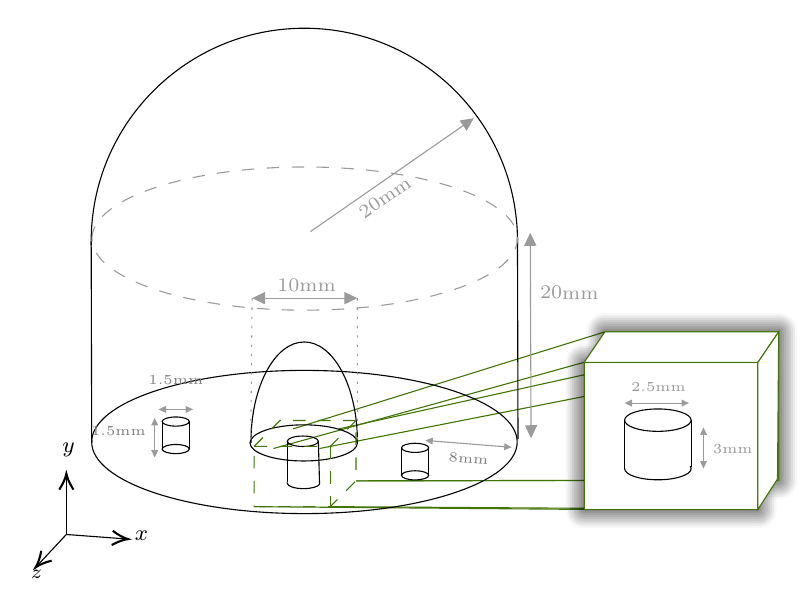
\begin{tikzpicture}[x=0.75pt,y=0.75pt,yscale=-1,xscale=1]
%uncomment if require: \path (0,324); %set diagram left start at 0, and has height of 324

%Straight Lines [id:da9524976530618017] 
\draw [color={rgb, 255:red, 65; green, 117; blue, 5 }  ,draw opacity=1 ]   (122.5,252.4) -- (281.5,253.73) ;
%Straight Lines [id:da49820750096655764] 
\draw [color={rgb, 255:red, 65; green, 117; blue, 5 }  ,draw opacity=1 ]   (159.16,252.4) -- (365.24,253.73) ;
%Straight Lines [id:da7065792347971342] 
\draw [color={rgb, 255:red, 65; green, 117; blue, 5 }  ,draw opacity=1 ]   (171.61,239.96) -- (375.24,239.73) ;
%Straight Lines [id:da8798365790071001] 
\draw [color={rgb, 255:red, 65; green, 117; blue, 5 }  ,draw opacity=1 ]   (171.61,239.96) -- (291.5,239.73) ;
%Straight Lines [id:da3792710550066729] 
\draw [color={rgb, 255:red, 65; green, 117; blue, 5 }  ,draw opacity=1 ]   (153.95,224.4) -- (365.24,182.86) ;
%Straight Lines [id:da9782944295344631] 
\draw [color={rgb, 255:red, 65; green, 117; blue, 5 }  ,draw opacity=1 ]   (131.83,224.4) -- (281.5,182.86) ;
%Straight Lines [id:da1518456627263618] 
\draw [color={rgb, 255:red, 65; green, 117; blue, 5 }  ,draw opacity=1 ]   (141.31,214.92) -- (291.5,168.19) ;
%Straight Lines [id:da941837570489849] 
\draw [color={rgb, 255:red, 65; green, 117; blue, 5 }  ,draw opacity=1 ]   (163.43,214.92) -- (375.24,168.19) ;
%Shape: Rectangle [id:dp6289718704196621] 
\draw  [color={rgb, 255:red, 65; green, 117; blue, 5 }  ,draw opacity=1 ][fill={rgb, 255:red, 255; green, 255; blue, 255 }  ,fill opacity=1 ][blur shadow={shadow xshift=0pt,shadow yshift=0pt, shadow blur radius=6.75pt, shadow blur steps=9 ,shadow opacity=100}] (291.5,168.19) -- (375.24,168.19) -- (375.24,239.73) -- (291.5,239.73) -- cycle ;
%Shape: Rectangle [id:dp30397440390041663] 
\draw  [color={rgb, 255:red, 65; green, 117; blue, 5 }  ,draw opacity=1 ][fill={rgb, 255:red, 255; green, 255; blue, 255 }  ,fill opacity=1 ][blur shadow={shadow xshift=0pt,shadow yshift=0pt, shadow blur radius=6.75pt, shadow blur steps=9 ,shadow opacity=100}] (281.5,182.86) -- (365.24,182.86) -- (365.24,253.73) -- (281.5,253.73) -- cycle ;
%Shape: Ellipse [id:dp37045868579866537] 
\draw   (44.25,221.25) .. controls (44.25,202.2) and (90.14,186.75) .. (146.75,186.75) .. controls (203.36,186.75) and (249.25,202.2) .. (249.25,221.25) .. controls (249.25,240.3) and (203.36,255.75) .. (146.75,255.75) .. controls (90.14,255.75) and (44.25,240.3) .. (44.25,221.25) -- cycle ;
%Shape: Arc [id:dp20060971662189897] 
\draw  [draw opacity=0] (120.98,221.7) .. controls (120.98,221.54) and (120.98,221.37) .. (120.98,221.21) .. controls (120.98,194.62) and (132.46,173.06) .. (146.63,173.06) .. controls (160.79,173.06) and (172.28,194.62) .. (172.28,221.21) .. controls (172.28,221.37) and (172.28,221.53) .. (172.28,221.69) -- (146.63,221.21) -- cycle ; \draw   (120.98,221.7) .. controls (120.98,221.54) and (120.98,221.37) .. (120.98,221.21) .. controls (120.98,194.62) and (132.46,173.06) .. (146.63,173.06) .. controls (160.79,173.06) and (172.28,194.62) .. (172.28,221.21) .. controls (172.28,221.37) and (172.28,221.53) .. (172.28,221.69) ;  
%Shape: Arc [id:dp782422935446454] 
\draw  [draw opacity=0] (44.02,126.48) .. controls (44.01,125.86) and (44,125.23) .. (44,124.6) .. controls (44,67.88) and (89.98,21.9) .. (146.7,21.9) .. controls (203.42,21.9) and (249.4,67.88) .. (249.4,124.6) .. controls (249.4,125.1) and (249.4,125.59) .. (249.39,126.09) -- (146.7,124.6) -- cycle ; \draw   (44.02,126.48) .. controls (44.01,125.86) and (44,125.23) .. (44,124.6) .. controls (44,67.88) and (89.98,21.9) .. (146.7,21.9) .. controls (203.42,21.9) and (249.4,67.88) .. (249.4,124.6) .. controls (249.4,125.1) and (249.4,125.59) .. (249.39,126.09) ;  
%Straight Lines [id:da96635676010308] 
\draw    (44,124.6) -- (44.25,221.25) ;
%Straight Lines [id:da2112067980893868] 
\draw    (249.39,123.24) -- (249.64,219.89) ;
%Shape: Ellipse [id:dp458676898897862] 
\draw  [draw opacity=0] (120.88,221.25) .. controls (120.88,216.44) and (132.46,212.54) .. (146.75,212.54) .. controls (161.04,212.54) and (172.62,216.44) .. (172.62,221.25) .. controls (172.62,226.06) and (161.04,229.96) .. (146.75,229.96) .. controls (132.46,229.96) and (120.88,226.06) .. (120.88,221.25) -- cycle ;
%Shape: Polygon [id:ds5597865340322787] 
\draw  [draw opacity=0] (84.73,213.6) -- (91.27,211.4) -- (91.27,224.65) -- (84.73,222.45) -- (78.19,224.65) -- (78.19,211.4) -- cycle ;
%Shape: Ellipse [id:dp7533297813492346] 
\draw   (78.19,211.4) .. controls (78.19,210.18) and (81.11,209.2) .. (84.73,209.2) .. controls (88.34,209.2) and (91.27,210.18) .. (91.27,211.4) .. controls (91.27,212.62) and (88.34,213.6) .. (84.73,213.6) .. controls (81.11,213.6) and (78.19,212.62) .. (78.19,211.4) -- cycle ;
%Shape: Ellipse [id:dp3087074759300781] 
\draw   (78.19,224.65) .. controls (78.19,223.44) and (81.11,222.45) .. (84.73,222.45) .. controls (88.34,222.45) and (91.27,223.44) .. (91.27,224.65) .. controls (91.27,225.87) and (88.34,226.85) .. (84.73,226.85) .. controls (81.11,226.85) and (78.19,225.87) .. (78.19,224.65) -- cycle ;
%Straight Lines [id:da9127417087811072] 
\draw    (91.27,211.4) -- (91.27,217.05) -- (91.27,224.65) ;
%Straight Lines [id:da758486436917319] 
\draw    (78.19,211.4) -- (78.19,224.65) ;
%Shape: Polygon [id:ds5726004508628542] 
\draw  [draw opacity=0] (145.98,223.41) -- (153.46,220.9) -- (153.46,236.05) -- (145.98,233.53) -- (138.5,236.05) -- (138.5,220.9) -- cycle ;
%Straight Lines [id:da24684899278609218] 
\draw    (138.5,220.9) -- (138.5,240.73) ;
%Straight Lines [id:da15150982673640367] 
\draw    (153.46,220.9) -- (154.03,241.64) ;
%Shape: Ellipse [id:dp14857116338846232] 
\draw   (138.5,220.9) .. controls (138.5,219.51) and (141.85,218.38) .. (145.98,218.38) .. controls (150.11,218.38) and (153.46,219.51) .. (153.46,220.9) .. controls (153.46,222.29) and (150.11,223.41) .. (145.98,223.41) .. controls (141.85,223.41) and (138.5,222.29) .. (138.5,220.9) -- cycle ;
%Shape: Ellipse [id:dp06650555705144767] 
\draw   (120.53,221.69) .. controls (120.53,216.88) and (132.11,212.98) .. (146.4,212.98) .. controls (160.69,212.98) and (172.28,216.88) .. (172.28,221.69) .. controls (172.28,226.5) and (160.69,230.4) .. (146.4,230.4) .. controls (132.11,230.4) and (120.53,226.5) .. (120.53,221.69) -- cycle ;
%Straight Lines [id:da9426142997164602] 
\draw [color={rgb, 255:red, 155; green, 155; blue, 155 }  ,draw opacity=1 ]   (74.61,212.68) -- (74.61,225.74) ;
\draw [shift={(74.61,228.74)}, rotate = 270] [fill={rgb, 255:red, 155; green, 155; blue, 155 }  ,fill opacity=1 ][line width=0.08]  [draw opacity=0] (3.57,-1.72) -- (0,0) -- (3.57,1.72) -- cycle    ;
\draw [shift={(74.61,209.68)}, rotate = 90] [fill={rgb, 255:red, 155; green, 155; blue, 155 }  ,fill opacity=1 ][line width=0.08]  [draw opacity=0] (3.57,-1.72) -- (0,0) -- (3.57,1.72) -- cycle    ;
%Straight Lines [id:da3906843086192191] 
\draw [color={rgb, 255:red, 155; green, 155; blue, 155 }  ,draw opacity=1 ]   (90.06,205.55) -- (79.49,205.55) ;
\draw [shift={(76.49,205.55)}, rotate = 360] [fill={rgb, 255:red, 155; green, 155; blue, 155 }  ,fill opacity=1 ][line width=0.08]  [draw opacity=0] (3.57,-1.72) -- (0,0) -- (3.57,1.72) -- cycle    ;
\draw [shift={(93.06,205.55)}, rotate = 180] [fill={rgb, 255:red, 155; green, 155; blue, 155 }  ,fill opacity=1 ][line width=0.08]  [draw opacity=0] (3.57,-1.72) -- (0,0) -- (3.57,1.72) -- cycle    ;
%Shape: Arc [id:dp7418376396627786] 
\draw  [draw opacity=0] (154.03,241.64) .. controls (153.25,242.83) and (150.1,243.72) .. (146.33,243.72) .. controls (141.97,243.72) and (138.44,242.53) .. (138.44,241.06) .. controls (138.44,240.95) and (138.46,240.84) .. (138.5,240.73) -- (146.33,241.06) -- cycle ; \draw   (154.03,241.64) .. controls (153.25,242.83) and (150.1,243.72) .. (146.33,243.72) .. controls (141.97,243.72) and (138.44,242.53) .. (138.44,241.06) .. controls (138.44,240.95) and (138.46,240.84) .. (138.5,240.73) ;  
%Shape: Ellipse [id:dp3833791898367582] 
\draw  [color={rgb, 255:red, 155; green, 155; blue, 155 }  ,draw opacity=1 ][dash pattern={on 4.5pt off 4.5pt}] (44.39,123.24) .. controls (44.39,104.18) and (90.28,88.74) .. (146.89,88.74) .. controls (203.5,88.74) and (249.39,104.18) .. (249.39,123.24) .. controls (249.39,142.29) and (203.5,157.74) .. (146.89,157.74) .. controls (90.28,157.74) and (44.39,142.29) .. (44.39,123.24) -- cycle ;
%Straight Lines [id:da5394046308099298] 
\draw [color={rgb, 255:red, 155; green, 155; blue, 155 }  ,draw opacity=1 ]   (149.64,119.89) -- (225.88,66.97) ;
\draw [shift={(228.34,65.26)}, rotate = 145.23] [fill={rgb, 255:red, 155; green, 155; blue, 155 }  ,fill opacity=1 ][line width=0.08]  [draw opacity=0] (6.25,-3) -- (0,0) -- (6.25,3) -- cycle    ;
%Straight Lines [id:da09576927903878119] 
\draw [color={rgb, 255:red, 155; green, 155; blue, 155 }  ,draw opacity=1 ]   (255.93,216.43) -- (255.55,123.46) ;
\draw [shift={(255.54,120.46)}, rotate = 89.77] [fill={rgb, 255:red, 155; green, 155; blue, 155 }  ,fill opacity=1 ][line width=0.08]  [draw opacity=0] (6.25,-3) -- (0,0) -- (6.25,3) -- cycle    ;
\draw [shift={(255.94,219.43)}, rotate = 269.77] [fill={rgb, 255:red, 155; green, 155; blue, 155 }  ,fill opacity=1 ][line width=0.08]  [draw opacity=0] (6.25,-3) -- (0,0) -- (6.25,3) -- cycle    ;
%Straight Lines [id:da3246746964570175] 
\draw [color={rgb, 255:red, 155; green, 155; blue, 155 }  ,draw opacity=1 ]   (169.21,151.96) -- (124.54,151.96) ;
\draw [shift={(121.54,151.96)}, rotate = 360] [fill={rgb, 255:red, 155; green, 155; blue, 155 }  ,fill opacity=1 ][line width=0.08]  [draw opacity=0] (6.25,-3) -- (0,0) -- (6.25,3) -- cycle    ;
\draw [shift={(172.21,151.96)}, rotate = 180] [fill={rgb, 255:red, 155; green, 155; blue, 155 }  ,fill opacity=1 ][line width=0.08]  [draw opacity=0] (6.25,-3) -- (0,0) -- (6.25,3) -- cycle    ;
%Straight Lines [id:da03118113260084332] 
\draw [color={rgb, 255:red, 155; green, 155; blue, 155 }  ,draw opacity=1 ] [dash pattern={on 0.84pt off 2.51pt}]  (121.54,151.96) -- (120.88,221.25) ;
%Straight Lines [id:da006336132751199486] 
\draw [color={rgb, 255:red, 155; green, 155; blue, 155 }  ,draw opacity=1 ] [dash pattern={on 0.84pt off 2.51pt}]  (172.21,151.96) -- (172.28,221.69) ;
%Straight Lines [id:da01853720670222203] 
\draw    (301,210.73) -- (301,234.07) ;
%Straight Lines [id:da0930152357666123] 
\draw    (333.05,210.73) -- (333.05,233.07) ;
%Straight Lines [id:da8870267403745837] 
\draw [color={rgb, 255:red, 155; green, 155; blue, 155 }  ,draw opacity=1 ]   (339,231) -- (339,217.25) ;
\draw [shift={(339,214.25)}, rotate = 90] [fill={rgb, 255:red, 155; green, 155; blue, 155 }  ,fill opacity=1 ][line width=0.08]  [draw opacity=0] (3.57,-1.72) -- (0,0) -- (3.57,1.72) -- cycle    ;
\draw [shift={(339,234)}, rotate = 270] [fill={rgb, 255:red, 155; green, 155; blue, 155 }  ,fill opacity=1 ][line width=0.08]  [draw opacity=0] (3.57,-1.72) -- (0,0) -- (3.57,1.72) -- cycle    ;
%Straight Lines [id:da8080201451770339] 
\draw [color={rgb, 255:red, 155; green, 155; blue, 155 }  ,draw opacity=1 ]   (304,202.5) -- (329,202.5) ;
\draw [shift={(332,202.5)}, rotate = 180] [fill={rgb, 255:red, 155; green, 155; blue, 155 }  ,fill opacity=1 ][line width=0.08]  [draw opacity=0] (3.57,-1.72) -- (0,0) -- (3.57,1.72) -- cycle    ;
\draw [shift={(301,202.5)}, rotate = 0] [fill={rgb, 255:red, 155; green, 155; blue, 155 }  ,fill opacity=1 ][line width=0.08]  [draw opacity=0] (3.57,-1.72) -- (0,0) -- (3.57,1.72) -- cycle    ;
%Shape: Ellipse [id:dp6313800829005536] 
\draw   (301,210.73) .. controls (301,207.75) and (308.17,205.33) .. (317.02,205.33) .. controls (325.87,205.33) and (333.05,207.75) .. (333.05,210.73) .. controls (333.05,213.7) and (325.87,216.12) .. (317.02,216.12) .. controls (308.17,216.12) and (301,213.7) .. (301,210.73) -- cycle ;
%Shape: Cube [id:dp17941447561191692] 
\draw  [color={rgb, 255:red, 65; green, 117; blue, 5 }  ,draw opacity=1 ][dash pattern={on 4.5pt off 4.5pt}] (122.5,223.36) -- (134.94,210.92) -- (171.61,210.92) -- (171.61,239.96) -- (159.16,252.4) -- (122.5,252.4) -- cycle ; \draw  [color={rgb, 255:red, 65; green, 117; blue, 5 }  ,draw opacity=1 ][dash pattern={on 4.5pt off 4.5pt}] (171.61,210.92) -- (159.16,223.36) -- (122.5,223.36) ; \draw  [color={rgb, 255:red, 65; green, 117; blue, 5 }  ,draw opacity=1 ][dash pattern={on 4.5pt off 4.5pt}] (159.16,223.36) -- (159.16,252.4) ;
%Shape: Polygon [id:ds6410027398322382] 
\draw  [color={rgb, 255:red, 65; green, 117; blue, 5 }  ,draw opacity=1 ][fill={rgb, 255:red, 255; green, 255; blue, 255 }  ,fill opacity=1 ] (291.5,168.19) -- (375.24,168.19) -- (365.24,182.86) -- (281.5,182.86) -- cycle ;
%Shape: Polygon [id:ds8811633029418593] 
\draw  [color={rgb, 255:red, 65; green, 117; blue, 5 }  ,draw opacity=1 ][fill={rgb, 255:red, 255; green, 255; blue, 255 }  ,fill opacity=1 ] (375.24,168.19) -- (374.67,239.07) -- (365.24,253.73) -- (365.24,182.86) -- cycle ;
%Straight Lines [id:da7676462536028303] 
\draw [color={rgb, 255:red, 155; green, 155; blue, 155 }  ,draw opacity=1 ]   (243.58,223.57) -- (207.99,220.74) ;
\draw [shift={(205,220.5)}, rotate = 4.55] [fill={rgb, 255:red, 155; green, 155; blue, 155 }  ,fill opacity=1 ][line width=0.08]  [draw opacity=0] (3.57,-1.72) -- (0,0) -- (3.57,1.72) -- cycle    ;
\draw [shift={(246.57,223.81)}, rotate = 184.55] [fill={rgb, 255:red, 155; green, 155; blue, 155 }  ,fill opacity=1 ][line width=0.08]  [draw opacity=0] (3.57,-1.72) -- (0,0) -- (3.57,1.72) -- cycle    ;
%Shape: Polygon [id:ds9095287089027209] 
\draw  [draw opacity=0] (200.06,226.27) -- (206.6,224.07) -- (206.6,237.32) -- (200.06,235.12) -- (193.52,237.32) -- (193.52,224.07) -- cycle ;
%Shape: Ellipse [id:dp5863481435378046] 
\draw   (193.52,224.07) .. controls (193.52,222.85) and (196.45,221.87) .. (200.06,221.87) .. controls (203.67,221.87) and (206.6,222.85) .. (206.6,224.07) .. controls (206.6,225.28) and (203.67,226.27) .. (200.06,226.27) .. controls (196.45,226.27) and (193.52,225.28) .. (193.52,224.07) -- cycle ;
%Shape: Ellipse [id:dp7930637252469577] 
\draw   (193.52,237.32) .. controls (193.52,236.1) and (196.45,235.12) .. (200.06,235.12) .. controls (203.67,235.12) and (206.6,236.1) .. (206.6,237.32) .. controls (206.6,238.53) and (203.67,239.52) .. (200.06,239.52) .. controls (196.45,239.52) and (193.52,238.53) .. (193.52,237.32) -- cycle ;
%Straight Lines [id:da44353809048931914] 
\draw    (206.6,224.07) -- (206.6,229.72) -- (206.6,237.32) ;
%Straight Lines [id:da9528011425410694] 
\draw    (193.52,224.07) -- (193.52,237.32) ;
%Shape: Arc [id:dp4442622677841004] 
\draw  [draw opacity=0] (332.65,232.87) .. controls (332.91,233.25) and (333.05,233.65) .. (333.05,234.07) .. controls (333.05,237.05) and (325.87,239.46) .. (317.02,239.46) .. controls (308.17,239.46) and (301,237.05) .. (301,234.07) -- (317.02,234.07) -- cycle ; \draw   (332.65,232.87) .. controls (332.91,233.25) and (333.05,233.65) .. (333.05,234.07) .. controls (333.05,237.05) and (325.87,239.46) .. (317.02,239.46) .. controls (308.17,239.46) and (301,237.05) .. (301,234.07) ;  
%Straight Lines [id:da2791889710789952] 
\draw    (32.04,238.53) -- (32.04,265.81) ;
\draw [shift={(32.04,236.53)}, rotate = 90] [color={rgb, 255:red, 0; green, 0; blue, 0 }  ][line width=0.75]    (7.65,-3.43) .. controls (4.86,-1.61) and (2.31,-0.47) .. (0,0) .. controls (2.31,0.47) and (4.86,1.61) .. (7.65,3.43)   ;
%Straight Lines [id:da8611093621202961] 
\draw    (59.8,267.88) -- (32.04,265.81) ;
\draw [shift={(61.79,268.03)}, rotate = 184.27] [color={rgb, 255:red, 0; green, 0; blue, 0 }  ][line width=0.75]    (7.65,-3.43) .. controls (4.86,-1.61) and (2.31,-0.47) .. (0,0) .. controls (2.31,0.47) and (4.86,1.61) .. (7.65,3.43)   ;
%Straight Lines [id:da054772923257707884] 
\draw    (18.57,280.21) -- (32.04,265.81) ;
\draw [shift={(17.21,281.67)}, rotate = 313.09] [color={rgb, 255:red, 0; green, 0; blue, 0 }  ][line width=0.75]    (7.65,-3.43) .. controls (4.86,-1.61) and (2.31,-0.47) .. (0,0) .. controls (2.31,0.47) and (4.86,1.61) .. (7.65,3.43)   ;

% Text Node
\draw (84.79,194.6) node [anchor=south] [inner sep=0.75pt]  [font=\small,color={rgb, 255:red, 128; green, 128; blue, 128 }  ,opacity=1 ] [align=left] {{\tiny 1.5mm}};
% Text Node
\draw (71.59,215.87) node [anchor=east] [inner sep=0.75pt]  [font=\small,color={rgb, 255:red, 128; green, 128; blue, 128 }  ,opacity=1 ] [align=left] {{\tiny 1.5mm}};
% Text Node
\draw (183.09,99.91) node [anchor=north] [inner sep=0.75pt]  [font=\scriptsize,color={rgb, 255:red, 155; green, 155; blue, 155 }  ,opacity=1 ,rotate=-325.37] [align=left] {20mm};
% Text Node
\draw (259.08,149.29) node [anchor=west] [inner sep=0.75pt]  [font=\scriptsize,color={rgb, 255:red, 155; green, 155; blue, 155 }  ,opacity=1 ,rotate=-0.5] [align=left] {20mm};
% Text Node
\draw (147.78,149.94) node [anchor=south] [inner sep=0.75pt]  [font=\scriptsize,color={rgb, 255:red, 155; green, 155; blue, 155 }  ,opacity=1 ,rotate=-0.5] [align=left] {10mm};
% Text Node
\draw (342.25,224.88) node [anchor=west] [inner sep=0.75pt]  [font=\tiny,color={rgb, 255:red, 155; green, 155; blue, 155 }  ,opacity=1 ]  {$\text{3mm}$};
% Text Node
\draw (317.3,198.3) node [anchor=south] [inner sep=0.75pt]  [font=\tiny,color={rgb, 255:red, 155; green, 155; blue, 155 }  ,opacity=1 ]  {$\text{2.5mm}$};
% Text Node
\draw (225.56,232.66) node [anchor=south] [inner sep=0.75pt]  [font=\small,color={rgb, 255:red, 128; green, 128; blue, 128 }  ,opacity=1 ,rotate=-4.32] [align=left] {{\tiny 8mm}};
% Text Node
\draw (33.14,229.88) node [anchor=south] [inner sep=0.75pt]  [font=\footnotesize]  {$y$};
% Text Node
\draw (63.75,266.58) node [anchor=west] [inner sep=0.75pt]  [font=\footnotesize]  {$x$};
% Text Node
\draw (13.67,284.95) node [anchor=west] [inner sep=0.75pt]  [font=\scriptsize]  {$z$};


\end{tikzpicture}

        %             \caption{}
        %             \label{fig:box-circle-3d:dimensions}
        %         \end{subfigure}
        %         \hfill
        %         \begin{subfigure}[b]{0.45\textwidth}
        %             \centering
        %             

\tikzset{every picture/.style={line width=0.75pt}} %set default line width to 0.75pt        

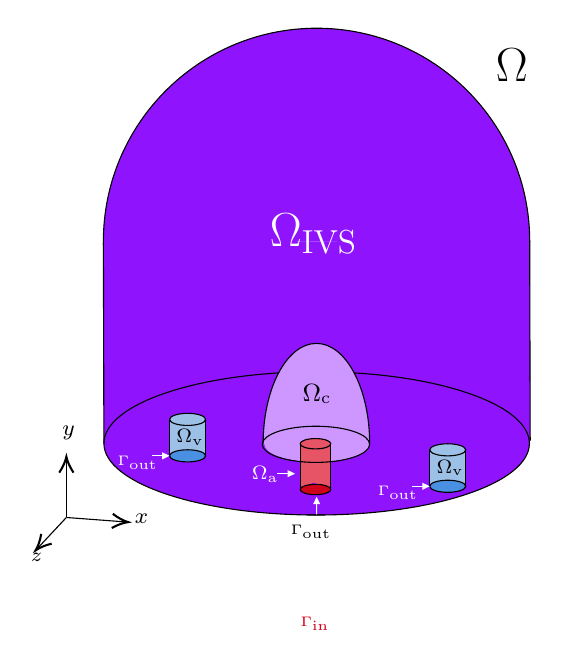
\begin{tikzpicture}[x=0.75pt,y=0.75pt,yscale=-1,xscale=1]
%uncomment if require: \path (0,300); %set diagram left start at 0, and has height of 300

%Shape: Polygon [id:ds01690740321670181] 
\draw  [draw opacity=0][fill={rgb, 255:red, 144; green, 19; blue, 254 }  ,fill opacity=1 ] (249.39,123.24) -- (249.64,219.89) -- (149,187.3) -- (44.25,221.25) -- (44,124.6) -- cycle ;
%Shape: Ellipse [id:dp07097539184655921] 
\draw  [fill={rgb, 255:red, 144; green, 19; blue, 254 }  ,fill opacity=1 ] (44.25,221.25) .. controls (44.25,202.2) and (90.14,186.75) .. (146.75,186.75) .. controls (203.36,186.75) and (249.25,202.2) .. (249.25,221.25) .. controls (249.25,240.3) and (203.36,255.75) .. (146.75,255.75) .. controls (90.14,255.75) and (44.25,240.3) .. (44.25,221.25) -- cycle ;
%Shape: Arc [id:dp2751562142003694] 
\draw  [draw opacity=0][fill={rgb, 255:red, 206; green, 150; blue, 255 }  ,fill opacity=1 ] (120.98,221.7) .. controls (120.98,221.54) and (120.98,221.37) .. (120.98,221.21) .. controls (120.98,194.62) and (132.46,173.06) .. (146.63,173.06) .. controls (160.79,173.06) and (172.28,194.62) .. (172.28,221.21) .. controls (172.28,221.37) and (172.28,221.53) .. (172.28,221.69) -- (146.63,221.21) -- cycle ; \draw   (120.98,221.7) .. controls (120.98,221.54) and (120.98,221.37) .. (120.98,221.21) .. controls (120.98,194.62) and (132.46,173.06) .. (146.63,173.06) .. controls (160.79,173.06) and (172.28,194.62) .. (172.28,221.21) .. controls (172.28,221.37) and (172.28,221.53) .. (172.28,221.69) ;  
%Shape: Polygon [id:ds05551048064302422] 
\draw  [draw opacity=0][fill={rgb, 255:red, 157; green, 192; blue, 231 }  ,fill opacity=1 ] (209.9,227.26) -- (218.57,224.34) -- (218.57,241.91) -- (209.9,238.99) -- (201.24,241.91) -- (201.24,224.34) -- cycle ;
%Straight Lines [id:da2434758497711771] 
\draw    (26.17,229.67) -- (26.17,256.94) ;
\draw [shift={(26.17,227.67)}, rotate = 90] [color={rgb, 255:red, 0; green, 0; blue, 0 }  ][line width=0.75]    (7.65,-3.43) .. controls (4.86,-1.61) and (2.31,-0.47) .. (0,0) .. controls (2.31,0.47) and (4.86,1.61) .. (7.65,3.43)   ;
%Straight Lines [id:da34708087552976474] 
\draw    (53.92,259.02) -- (26.17,256.94) ;
\draw [shift={(55.92,259.17)}, rotate = 184.27] [color={rgb, 255:red, 0; green, 0; blue, 0 }  ][line width=0.75]    (7.65,-3.43) .. controls (4.86,-1.61) and (2.31,-0.47) .. (0,0) .. controls (2.31,0.47) and (4.86,1.61) .. (7.65,3.43)   ;
%Straight Lines [id:da30935515392198853] 
\draw    (12.7,271.34) -- (26.17,256.94) ;
\draw [shift={(11.33,272.8)}, rotate = 313.09] [color={rgb, 255:red, 0; green, 0; blue, 0 }  ][line width=0.75]    (7.65,-3.43) .. controls (4.86,-1.61) and (2.31,-0.47) .. (0,0) .. controls (2.31,0.47) and (4.86,1.61) .. (7.65,3.43)   ;
%Shape: Arc [id:dp4353496030990409] 
\draw  [draw opacity=0][fill={rgb, 255:red, 144; green, 19; blue, 254 }  ,fill opacity=1 ] (44.01,125.8) .. controls (44,125.17) and (44,124.55) .. (44,123.92) .. controls (44,67.2) and (89.98,21.22) .. (146.7,21.22) .. controls (203.42,21.22) and (249.4,67.2) .. (249.4,123.92) .. controls (249.4,124.42) and (249.39,124.91) .. (249.39,125.41) -- (146.7,123.92) -- cycle ; \draw   (44.01,125.8) .. controls (44,125.17) and (44,124.55) .. (44,123.92) .. controls (44,67.2) and (89.98,21.22) .. (146.7,21.22) .. controls (203.42,21.22) and (249.4,67.2) .. (249.4,123.92) .. controls (249.4,124.42) and (249.39,124.91) .. (249.39,125.41) ;  
%Straight Lines [id:da13806152488339984] 
\draw    (44,124.6) -- (44.25,221.25) ;
%Straight Lines [id:da6383479755639994] 
\draw    (249.39,123.24) -- (249.64,219.89) ;
%Shape: Ellipse [id:dp9307891644906987] 
\draw  [fill={rgb, 255:red, 157; green, 192; blue, 231 }  ,fill opacity=1 ] (201.24,224.34) .. controls (201.24,222.73) and (205.12,221.43) .. (209.9,221.43) .. controls (214.69,221.43) and (218.57,222.73) .. (218.57,224.34) .. controls (218.57,225.95) and (214.69,227.26) .. (209.9,227.26) .. controls (205.12,227.26) and (201.24,225.95) .. (201.24,224.34) -- cycle ;
%Shape: Ellipse [id:dp9565465123212877] 
\draw  [fill={rgb, 255:red, 74; green, 144; blue, 226 }  ,fill opacity=1 ] (201.24,241.91) .. controls (201.24,240.29) and (205.12,238.99) .. (209.9,238.99) .. controls (214.69,238.99) and (218.57,240.29) .. (218.57,241.91) .. controls (218.57,243.52) and (214.69,244.82) .. (209.9,244.82) .. controls (205.12,244.82) and (201.24,243.52) .. (201.24,241.91) -- cycle ;
%Shape: Ellipse [id:dp9395551579921961] 
\draw  [draw opacity=0][fill={rgb, 255:red, 206; green, 150; blue, 255 }  ,fill opacity=1 ] (121.57,221.69) .. controls (121.57,216.98) and (132.92,213.16) .. (146.92,213.16) .. controls (160.93,213.16) and (172.28,216.98) .. (172.28,221.69) .. controls (172.28,226.4) and (160.93,230.23) .. (146.92,230.23) .. controls (132.92,230.23) and (121.57,226.4) .. (121.57,221.69) -- cycle ;
%Straight Lines [id:da37394575581946365] 
\draw    (218.57,224.34) -- (218.57,241.91) ;
%Straight Lines [id:da5923482443180503] 
\draw    (201.24,224.34) -- (201.24,241.91) ;
%Shape: Polygon [id:ds36655981362937773] 
\draw  [draw opacity=0][fill={rgb, 255:red, 231; green, 84; blue, 102 }  ,fill opacity=1 ] (146.19,223.89) -- (153.57,221.41) -- (153.57,243.47) -- (145.22,240.09) -- (138.8,243.47) -- (138.8,221.41) -- cycle ;
%Straight Lines [id:da12421975552257325] 
\draw    (138.8,221.41) -- (138.8,243.47) ;
%Straight Lines [id:da06433371565445012] 
\draw    (153.57,221.41) -- (153.57,243.47) ;
%Shape: Ellipse [id:dp9306496239950879] 
\draw  [fill={rgb, 255:red, 231; green, 84; blue, 102 }  ,fill opacity=1 ] (138.8,221.41) .. controls (138.8,220.04) and (142.11,218.92) .. (146.19,218.92) .. controls (150.26,218.92) and (153.57,220.04) .. (153.57,221.41) .. controls (153.57,222.78) and (150.26,223.89) .. (146.19,223.89) .. controls (142.11,223.89) and (138.8,222.78) .. (138.8,221.41) -- cycle ;
%Straight Lines [id:da9919027107135354] 
\draw [color={rgb, 255:red, 255; green, 255; blue, 255 }  ,draw opacity=1 ]   (133.33,235.83) -- (127.67,235.83) ;
\draw [shift={(136.33,235.83)}, rotate = 180] [fill={rgb, 255:red, 255; green, 255; blue, 255 }  ,fill opacity=1 ][line width=0.08]  [draw opacity=0] (3.57,-1.72) -- (0,0) -- (3.57,1.72) -- cycle    ;
%Shape: Ellipse [id:dp6340587055082747] 
\draw   (120.53,221.69) .. controls (120.53,216.88) and (132.11,212.98) .. (146.4,212.98) .. controls (160.69,212.98) and (172.28,216.88) .. (172.28,221.69) .. controls (172.28,226.5) and (160.69,230.4) .. (146.4,230.4) .. controls (132.11,230.4) and (120.53,226.5) .. (120.53,221.69) -- cycle ;
%Straight Lines [id:da4747494457620296] 
\draw [color={rgb, 255:red, 255; green, 255; blue, 255 }  ,draw opacity=1 ]   (198.24,241.91) -- (192.57,241.91) ;
\draw [shift={(201.24,241.91)}, rotate = 180] [fill={rgb, 255:red, 255; green, 255; blue, 255 }  ,fill opacity=1 ][line width=0.08]  [draw opacity=0] (3.57,-1.72) -- (0,0) -- (3.57,1.72) -- cycle    ;
%Shape: Polygon [id:ds6448294514764339] 
\draw  [draw opacity=0][fill={rgb, 255:red, 157; green, 192; blue, 231 }  ,fill opacity=1 ] (84.57,212.59) -- (93.24,209.68) -- (93.24,227.24) -- (84.57,224.32) -- (75.9,227.24) -- (75.9,209.68) -- cycle ;
%Shape: Ellipse [id:dp5042958695035071] 
\draw  [fill={rgb, 255:red, 157; green, 192; blue, 231 }  ,fill opacity=1 ] (75.9,209.68) .. controls (75.9,208.07) and (79.78,206.76) .. (84.57,206.76) .. controls (89.36,206.76) and (93.24,208.07) .. (93.24,209.68) .. controls (93.24,211.29) and (89.36,212.59) .. (84.57,212.59) .. controls (79.78,212.59) and (75.9,211.29) .. (75.9,209.68) -- cycle ;
%Shape: Ellipse [id:dp621045676508921] 
\draw  [fill={rgb, 255:red, 74; green, 144; blue, 226 }  ,fill opacity=1 ] (75.9,227.24) .. controls (75.9,225.63) and (79.78,224.32) .. (84.57,224.32) .. controls (89.36,224.32) and (93.24,225.63) .. (93.24,227.24) .. controls (93.24,228.85) and (89.36,230.16) .. (84.57,230.16) .. controls (79.78,230.16) and (75.9,228.85) .. (75.9,227.24) -- cycle ;
%Straight Lines [id:da6241652370301061] 
\draw    (93.24,209.68) -- (93.24,227.24) ;
%Straight Lines [id:da7595036939515529] 
\draw    (75.9,209.68) -- (75.9,227.24) ;
%Straight Lines [id:da6580144119581173] 
\draw [color={rgb, 255:red, 255; green, 255; blue, 255 }  ,draw opacity=1 ]   (72.9,227.24) -- (67.24,227.24) ;
\draw [shift={(75.9,227.24)}, rotate = 180] [fill={rgb, 255:red, 255; green, 255; blue, 255 }  ,fill opacity=1 ][line width=0.08]  [draw opacity=0] (3.57,-1.72) -- (0,0) -- (3.57,1.72) -- cycle    ;
%Straight Lines [id:da516421428956964] 
\draw [color={rgb, 255:red, 255; green, 255; blue, 255 }  ,draw opacity=1 ]   (146.76,249.98) -- (146.75,255.75) ;
\draw [shift={(146.76,246.98)}, rotate = 90.08] [fill={rgb, 255:red, 255; green, 255; blue, 255 }  ,fill opacity=1 ][line width=0.08]  [draw opacity=0] (3.57,-1.72) -- (0,0) -- (3.57,1.72) -- cycle    ;
%Shape: Arc [id:dp001845141988116028] 
\draw  [draw opacity=0] (150.65,255.68) .. controls (149.31,255.7) and (147.97,255.71) .. (146.63,255.71) .. controls (144.98,255.71) and (143.34,255.7) .. (141.7,255.67) -- (146.63,221.21) -- cycle ; \draw   (150.65,255.68) .. controls (149.31,255.7) and (147.97,255.71) .. (146.63,255.71) .. controls (144.98,255.71) and (143.34,255.7) .. (141.7,255.67) ;  
%Shape: Ellipse [id:dp7362360871362295] 
\draw  [fill={rgb, 255:red, 208; green, 2; blue, 27 }  ,fill opacity=1 ] (138.8,243.47) .. controls (138.8,242.1) and (142.11,240.98) .. (146.19,240.98) .. controls (150.26,240.98) and (153.57,242.1) .. (153.57,243.47) .. controls (153.57,244.84) and (150.26,245.95) .. (146.19,245.95) .. controls (142.11,245.95) and (138.8,244.84) .. (138.8,243.47) -- cycle ;

% Text Node
\draw (27.27,221.01) node [anchor=south] [inner sep=0.75pt]  [font=\footnotesize]  {$y$};
% Text Node
\draw (57.88,257.72) node [anchor=west] [inner sep=0.75pt]  [font=\footnotesize]  {$x$};
% Text Node
\draw (7.79,276.08) node [anchor=west] [inner sep=0.75pt]  [font=\scriptsize]  {$z$};
% Text Node
\draw (145.32,120.23) node  [font=\LARGE,color={rgb, 255:red, 255; green, 255; blue, 255 }  ,opacity=1 ]  {$\Omega _{\text{IVS}}$};
% Text Node
\draw (146.92,197.43) node  [font=\small,color={rgb, 255:red, 0; green, 0; blue, 0 }  ,opacity=1 ]  {$\Omega _{\text{c}}$};
% Text Node
\draw (129.63,236.34) node [anchor=east] [inner sep=0.75pt]  [font=\scriptsize,color={rgb, 255:red, 255; green, 255; blue, 255 }  ,opacity=1 ]  {$\Omega _{\text{a}}$};
% Text Node
\draw (211.09,233.02) node  [font=\scriptsize,color={rgb, 255:red, 0; green, 0; blue, 0 }  ,opacity=1 ]  {$\Omega _{\text{v}}$};
% Text Node
\draw (240.82,39.23) node  [font=\LARGE,color={rgb, 255:red, 0; green, 0; blue, 0 }  ,opacity=1 ]  {$\Omega $};
% Text Node
\draw (145.93,303.53) node [anchor=north] [inner sep=0.75pt]  [font=\tiny,color={rgb, 255:red, 208; green, 2; blue, 27 }  ,opacity=1 ]  {$\Gamma _{\text{in}}$};
% Text Node
\draw (196.83,240.77) node [anchor=north east] [inner sep=0.75pt]  [font=\tiny,color={rgb, 255:red, 255; green, 255; blue, 255 }  ,opacity=1 ]  {$\Gamma _{\text{out}}$};
% Text Node
\draw (85.75,218.35) node  [font=\scriptsize,color={rgb, 255:red, 0; green, 0; blue, 0 }  ,opacity=1 ]  {$\Omega _{\text{v}}$};
% Text Node
\draw (71.5,226.1) node [anchor=north east] [inner sep=0.75pt]  [font=\tiny,color={rgb, 255:red, 255; green, 255; blue, 255 }  ,opacity=1 ]  {$\Gamma _{\text{out}}$};
% Text Node
\draw (155,268.36) node [anchor=south east] [inner sep=0.75pt]  [font=\tiny,color={rgb, 255:red, 0; green, 0; blue, 0 }  ,opacity=1 ]  {$\Gamma _{\text{out}}$};


\end{tikzpicture}

        %             \caption{}
        %             \label{fig:box-circle-3d:regions}
        %         \end{subfigure}
        %         \caption{Not to scale. (a) Diagram illustrating a simple 3D placentone geometry with dimensions. Red shows the inlet location and blue shows outlet locations. (b) Diagram illustrating subdomains with $\Omega$.}
        %         \label{fig:box-circle-3d}
        %     \end{figure}

    \section{Blood flow model} \label{sec:modelling:blood-flow}        
        Previous authors using macro-scale models for maternal blood flow take flow through the villous tree as porous flow, and to treat other flows as `free' flow. Here, we will introduce a model that respects this approach, and make comparisons to other popular choices in the literature \cite{lecarpentierComputationalFluidDynamic2016,chernyavskyMathematicalModelIntervillous2010,meklerImpactTissuePorosity2022,erianMaternalPlacentalBlood1977,saghianAssociationPlacentalJets2017} in \S\ref{sec:modelling:blood-flow:s+b} and \ref{sec:modelling:blood-flow:ns+nsb}.
            
        One of the main contributions of this thesis is to use the Navier-Stokes-Darcy (NSD) equations to model maternal blood flow on a 2D placenta geometry. Whilst there is work that uses NSD and related models \cite{angotPenalizationMethodTake1999,fuchsbergerIncorporationObstaclesFluid2022,engelsFluSINovelParallel2016,jiaModelingAnalysisCarbonate2021}, as far as we are aware there is only one work that uses a single Navier-Stokes-type PDE to model flow in the context of the placenta \cite{meklerImpactTissuePorosity2022}. This approach is advantageous for the numerical methods we will employ, gives a physiologically sensible transition region between `free' and porous flow, and avoids non-physical boundary layers that may occur when coupling, for example, the Navier-Stokes and Brinkman equations \cite{brinkmanCalculationViscousForce1949}. To be clear, our model of maternal blood flow is: find $\vec{u}, p$ such that
        \begin{subequations}
            \begin{align}
                \begin{split}
                    \rho \pdv{\vec{u}}{t} + \Psi \frac{\mu}{k} \vec{u} + \rho (\vec{u} \cdot \vec{\nabla}) \vec{u} - \mu \nabla^2 \vec{u} + \vec{\nabla} p = \vec{f}_\text{f} &~ \text{in } \Omega,
                    \label{eq:nsb:momentum}
                \end{split}\\
                \begin{split}
                    \vec{\nabla} \cdot \vec{u} = 0 &~ \text{in } \Omega,
                    \label{eq:nsb:incompressibility}%
                \end{split}%
            \end{align}%
            \label{eq:nsb}%
        \end{subequations}%
        where the problem is supplemented with a suitable initial condition and boundary conditions (to be given in \S\ref{sec:modelling:blood-flow:boundary-conditions}), $\rho$ is the density of the fluid, $\mu$ is the dynamic viscosity, $\vec{f}_\text{f}$ is a body force acting on the flow, and the coefficient of the reaction term varies spatially, i.e., $\Psi(\vec{x}) \frac{\mu}{k}$. We assign $\Psi = 1$ in areas of villous tree, $\Psi = 0$ in areas of no villous tree, with a smooth transition on the region in between. The shape of this smooth transition follows a $\tanh$ profile. Figure \ref{fig:permeability} illustrates an example of the profile of $\Psi$ in the placentone geometry, and Appendix \ref{sec:smooth-transition} contains the details on the precise definition of this function.

        \begin{figure}
            \centering
            

\tikzset{every picture/.style={line width=0.75pt}} %set default line width to 0.75pt        

\begin{tikzpicture}[x=0.75pt,y=0.75pt,yscale=-1,xscale=1]
%uncomment if require: \path (0,300); %set diagram left start at 0, and has height of 300

%Shape: Rectangle [id:dp05948589068926391] 
\draw  [color={rgb, 255:red, 144; green, 19; blue, 254 }  ,draw opacity=1 ][fill={rgb, 255:red, 255; green, 255; blue, 255 }  ,fill opacity=1 ][line width=2.25] [blur shadow={shadow xshift=0pt,shadow yshift=0pt, shadow blur radius=1.5pt, shadow blur steps=4 ,shadow opacity=100}] (23,74.5) -- (160,74.5) -- (160,218) -- (23,218) -- cycle ;
%Image [id:dp5741033059414491] 
\draw (279.44,145.67) node  {\includegraphics[width=142.91pt,height=214.5pt]{diagrams/results-modelling/velocity-transport/meshandsoln_cg_permeability_placenta_nsb_permeability-linear.png}};
%Image [id:dp5031667319380262] 
\draw (90.5,171.72) node  {\includegraphics[width=82.5pt,height=123.83pt]{diagrams/results-modelling/velocity-transport/meshandsoln_cg_permeability_placenta_nsb_permeability-linear_vein.png}};
%Shape: Polygon [id:ds7395586031334473] 
\draw  [fill={rgb, 255:red, 155; green, 155; blue, 155 }  ,fill opacity=0.2 ] (421.25,250.25) -- (317,245.5) -- (317,120) -- (421.25,23) -- cycle ;
%Shape: Rectangle [id:dp1357774358505115] 
\draw   (240.75,120) -- (317,120) -- (317,245.5) -- (240.75,245.5) -- cycle ;
%Shape: Rectangle [id:dp02134536760375405] 
\draw  [color={rgb, 255:red, 144; green, 19; blue, 254 }  ,draw opacity=1 ][fill={rgb, 255:red, 255; green, 255; blue, 255 }  ,fill opacity=1 ][line width=2.25] [blur shadow={shadow xshift=0pt,shadow yshift=0pt, shadow blur radius=1.5pt, shadow blur steps=4 ,shadow opacity=100}] (421.25,23) -- (576.5,23) -- (576.5,250.5) -- (421.25,250.5) -- cycle ;
%Image [id:dp27582567302078576] 
\draw (497.74,131.58) node  {\includegraphics[width=101.85pt,height=152.88pt]{diagrams/results-modelling/velocity-transport/meshandsoln_cg_permeability_placenta_nsb_permeability-linear_cavity.png}};
%Shape: Polygon [id:ds4671748834121485] 
\draw  [fill={rgb, 255:red, 155; green, 155; blue, 155 }  ,fill opacity=0.2 ] (217.75,202.5) -- (160,218) -- (160,74.5) -- (217.75,186.5) -- cycle ;
%Shape: Rectangle [id:dp28400651386966036] 
\draw   (217.75,186.5) -- (231,186.5) -- (231,202.5) -- (217.75,202.5) -- cycle ;




\end{tikzpicture}

            \caption{Diagram illustrating $\Psi$ on a placentone as described in \S\ref{sec:modelling:blood-flow}. Blue regions correspond to $\Psi = 0$ and red regions correspond to $\Psi = 1$. The definition of $\Psi$ is formally presented in Appendix \ref{sec:smooth-transition}. The value is dependent upon the subregions of $\Omega$ and transition sizes that are illustrated in Figure \ref{fig:box-circle}.}
            \label{fig:permeability}
        \end{figure}
            
        Through the remainder of \S\ref{sec:modelling:blood-flow}, we will define two alternative blood flow models, as these form common choices in the current literature, and present the boundary conditions and parameters we will use in these problems. Approximations to these problems will then be compared later in \S\ref{sec:numerical-methods:blood-flow-experiments}; for simplicity, these comparisons will consider only the steady-state equations. We will consider:
        \begin{itemize}
            \item \S\ref{sec:modelling:blood-flow:boundary-conditions}: Boundary conditions and model parameters common to all flow problems,
            \item \S\ref{sec:modelling:blood-flow:s+b}: Brinkman in $\Omega_\text{IVS} \cup \Omega_{T^+}$ and Stokes in $\Omega \setminus (\Omega_\text{IVS} \cup \Omega_{T^+})$,
            \item \S\ref{sec:modelling:blood-flow:ns+nsb}: Navier-Stokes-Darcy in $\Omega_\text{IVS} \cup \Omega_{T^+}$ and Navier-Stokes in $\Omega \setminus (\Omega_\text{IVS} \cup \Omega_{T^+})$.
        \end{itemize}

        \subsection{Boundary conditions and placenta parameters} \label{sec:modelling:blood-flow:boundary-conditions}
            For all velocity model choices, we prescribe the same boundary conditions: a parabolic inflow velocity profile, with a `directional do-nothing' condition on outflow, and no velocity slip elsewhere. These choices correspond to boundary conditions of the form
            \begin{subequations}
                \begin{alignat*}{3}
                    \left( \mu \nabla \vec{u} - p \mat{I} \right) \cdot \vec{n} & = \vec{g}_\text{f,N} &&~ \text{on } \Gamma_\text{out}, \\
                    \vec{u} & = \vec{g}_\text{f,D} &&~ \text{on } \Gamma\setminus\Gamma_\text{out},
                \end{alignat*}%
            \end{subequations}%
            where $\Gamma := \partial \Omega$ is labelled in Figures \ref{fig:box-circle:regions} and \ref{fig:inverted-circle-slice-6-flat:regions}, and $\vec{n}(\vec{x})$ is the unit outward-pointing normal at a point $\vec{x}$. We note that the outflow condition is a common choice used in the numerics community \cite{griffiths_no_1997,renardy_imposing_1997}. The boundary conditions themselves are given by
            \begin{subequations}
                \begin{alignat}{3}
                    \vec{g}_\text{f,D} & = - U \frac{R^2 - r^2}{R^2} \vec{n} &&~ \text{on } \Gamma_\text{in},\label{eq:velocity-bcs:dirichlet-parabola}\\
                    \vec{g}_\text{f,N} & = \vec{0} &&~ \text{on } \Gamma_\text{out},\label{eq:velocity-bcs:neumann}\\
                    \vec{g}_\text{f,D} & = \vec{0} &&~ \text{on } \Gamma \setminus (\Gamma_\text{in} \cup \Gamma_\text{out}),\label{eq:velocity-bcs:dirichlet-no-slip}
                \end{alignat}%
                \label{eq:velocity-bcs}%
            \end{subequations}%
            where $\vec{n}$ is the unit outward-pointing normal on $\Gamma_\text{in}$, $r(\vec{x})$ is the distance to from a point $\vec{x}$ to the centre of $\Gamma_\text{in}$, $R$ is the artery radius, and $U$ is the maximum flow amplitude at the centre of the inlet.

            Tables \ref{tab:structural-parameters} and \ref{tab:problem-parameters} give lists of parameters used throughout this thesis' analyses, where the nominal values listed are used in all simulations unless otherwise stated.

            \begin{table}
                \centering
                \begin{adjustwidth}{-1.5cm}{-1cm}
                    \begin{tabular}{c|c|c|c|c}
                        Parameter & Description & Nominal value & Range & Reference \\
                        \hline
                        $b_1, a_1$ & Axes of central cavity & \qtylist{10;5}{\milli\metre} & — & \cite{lecarpentierComputationalFluidDynamic2016} \\
                        — & Artery location & \qty{20}{\milli\metre} (from side) & — & \cite{chernyavskyMathematicalModelIntervillous2010,lecarpentierComputationalFluidDynamic2016} \\
                        — & Vein location & \qty{8}{\milli\metre} (from side) & — & \cite{chernyavskyMathematicalModelIntervillous2010,lecarpentierComputationalFluidDynamic2016} \\
                        $2r_a$ & Artery width (mouth) & \qty{2.4}{\milli\metre} & \qtyrange{0.5}{3}{\milli\metre} & \cite{burtonRheologicalPhysiologicalConsequences2009} \\
                        — & Artery width (upstream) & \qty{0.5}{\milli\metre} & — & \cite{burtonRheologicalPhysiologicalConsequences2009} \\
                        $2r_v$ & Vein width & \qty{1.5}{\milli\metre} & — & — \\
                        $2r^\text{ms}_v$ & Marginal sinus vein width & \qty{3}{\milli\metre} & — & — \\
                        — & Central cavity width & \qty{10}{\milli\metre} & — & \cite{lecarpentierComputationalFluidDynamic2016,chernyavskyMathematicalModelIntervillous2010} \\
                        $\tau$ & Central cavity transition & \qty{4.8}{\milli\metre} & — & — \\
                        — & Vein transition & \qty{1.2}{\milli\metre} & — & — \\
                        — & Small septal wall heights & \qty{6.90}{\milli\metre} & \qtyrange{5.26}{9.54}{\milli\metre} & \cite{AMANITIS2023e68} \\
                        — & Tall septal wall heights & \qty{14.07}{\milli\metre} & \qtyrange{12.15}{17.75}{\milli\metre} & \cite{AMANITIS2023e68} \\
                        — & Number of arteries (3D) & — & $30$—$150$ & \cite{benirschkePathologyHumanPlacenta2012,chernyavskyMathematicalModelIntervillous2010,burtonRheologicalPhysiologicalConsequences2009} \\
                        — & Number of veins (3D) & — & $50$—$200$ & \cite{chernyavskyMathematicalModelIntervillous2010} \\
                        — & Number of placentones (3D) & — & $30$—$60$ & \cite{benirschkePathologyHumanPlacenta2012,serovRoleMorphologyMathematical2016} \\
                    \end{tabular}
                \end{adjustwidth}
                \caption{Placental structural parameter nominal values and ranges found in the placental literature.}
                \label{tab:structural-parameters}
            \end{table}

            \begin{table}
                \centering
                \begin{adjustwidth}{-1.5cm}{-1cm}
                    \begin{tabular}{c|c|c|c|c}
                        \centering
                        Parameter & Description & Nominal value & Range & Reference \\
                        \hline
                        $L$ & Placentone width & \qty{4e-2}{\metre} & \qtyrange{1e-2}{4e-2}{\metre} & \cite{chernyavskyMathematicalModelIntervillous2010,lecarpentierComputationalFluidDynamic2016} \\
                        $k$ & Villous tree permeability & \qty{1e-8}{\metre^2} & \qtyrange{1e-6}{1e-10}{\metre^2} & \cite{lecarpentierComputationalFluidDynamic2016,chernyavskyMathematicalModelIntervillous2010} \\
                        $\mu$ & Blood viscosity & \qty{4e-3}{\pascal\second} & — & \cite{chernyavskyMathematicalModelIntervillous2010} \\
                        $\rho$ & Blood density & \qty{1e3}{\kilogram\per\metre^3} & — & \cite{chernyavskyMathematicalModelIntervillous2010} \\
                        $D$ & Oxygen diffusivity & \qty{1.667e-5}{\metre^2\per\second} & \qtyrange{1e-5}{1.667e-5}{\metre^2\per\second} & \cite{chernyavskyMathematicalModelIntervillous2010,banerjeeCoupledOxygenTransport2008} \\
                        $R$ & Oxygen uptake & \qty{1.667e-2}{\per\second} & — & \cite{chernyavskyMathematicalModelIntervillous2010} \\
                        — & Artery blood speed (mouth) & \qty{0.1}{\metre\per\second} & \qtyrange{0.037}{0.3}{\metre\per\second} & \cite{burtonRheologicalPhysiologicalConsequences2009,chernyavskyMathematicalModelIntervillous2010,kurjakDopplerAssessmentIntervillous1997,collinsDevelopmentalChangesSpiral2012} \\
                        $U$ & Artery blood speed (upstream) & \qty{0.35}{\metre\per\second}\anote & \qtyrange{0.5}{4}{\metre\per\second} & \cite{burtonRheologicalPhysiologicalConsequences2009,saghianAssociationPlacentalJets2017,chernyavskyMathematicalModelIntervillous2010} \\
                    \end{tabular}
                \end{adjustwidth}
                \caption{Maternal blood parameter nominal values and ranges found in the placental literature. \anote The upstream speed of \qty{0.35}{\metre\per\second} was selected such that flow at the mouth is approximately \qty{0.1}{\metre\per\second}.}
                \label{tab:problem-parameters}
            \end{table}

            \S\ref{sec:modelling:blood-flow:s+b} and \S\ref{sec:modelling:blood-flow:ns+nsb} will now outline two alternative models of maternal blood flow, taken directly from, or closely related to, those chosen in the literature.

        \subsection{Stokes and Brinkman (S-B)} \label{sec:modelling:blood-flow:s+b}
            We solve Brinkman in the IVS, and Stokes elsewhere: find $\vec{u}, p$ such that
            \begin{subequations}
                \begin{align}
                    \begin{split}
                        \frac{\mu}{k} \vec{u} -\mu\nabla^2 \vec{u} + \vec{\nabla} p = \vec{0} &~ \text{in } \Omega_{\text{IVS}} \cup \Omega_{T^+},
                    \end{split}\\
                    \begin{split}
                        -\mu\nabla^2 \vec{u} + \vec{\nabla} p = \vec{0} &~ \text{in } \Omega \setminus (\Omega_{\text{IVS}} \cup \Omega_{T^+}),
                    \end{split}\\
                    \begin{split}
                        \vec{\nabla} \cdot \vec{u} = 0 &~ \text{in } \Omega,
                    \end{split}%
                \end{align}%
                \label{eq:s-b}%
            \end{subequations}%
            with boundary conditions given in Equation \ref{eq:velocity-bcs}. This is the simplest of the three velocity models, and the only model which is linear everywhere. This model is related to work by \citeauthor{chernyavskyMathematicalModelIntervillous2010} \cite{chernyavskyMathematicalModelIntervillous2010} and \citeauthor{erianMaternalPlacentalBlood1977} \cite{erianMaternalPlacentalBlood1977} who use Darcy's law. We opted to use the Brinkman equation instead of Darcy's law in the porous region for two reasons: firstly, Brinkman captures the drag effects associated with resistance of flow through the villous tree, and secondly, allows for simple application of interface conditions due to both equations being of the same order \cite{brinkmanCalculationViscousForce1949}. 

        \subsection{Navier-Stokes and Navier-Stokes-Darcy (NS-NSD)} \label{sec:modelling:blood-flow:ns+nsb}
            We solve steady-state Navier-Stokes-Darcy in the IVS, and steady-state Navier-Stokes elsewhere: find $\vec{u}, p$ such that
            \begin{subequations}
                \begin{align}
                    \begin{split}
                        \frac{\mu}{k}\vec{u} + \rho (\vec{u} \cdot \vec{\nabla}) \vec{u} - \mu \nabla^2 \vec{u} + \vec{\nabla} p = \vec{0} &~ \text{in } \Omega_{\text{IVS}} \cup \Omega_{T^+},
                    \end{split}\\
                    \begin{split}
                        \rho (\vec{u} \cdot \vec{\nabla}) \vec{u} - \mu \nabla^2 \vec{u} + \vec{\nabla} p = \vec{0} &~ \text{in } \Omega \setminus (\Omega_{\text{IVS}} \cup \Omega_{T^+}),
                    \end{split}\\
                    \begin{split}
                        \vec{\nabla} \cdot \vec{u} = 0 &~ \text{in } \Omega,
                    \end{split}%
                \end{align}%
                \label{eq:ns-nsb}%
            \end{subequations}%
            with boundary conditions given in Equation \ref{eq:velocity-bcs}. This example follows work by \citeauthor{lecarpentierComputationalFluidDynamic2016} \cite{lecarpentierComputationalFluidDynamic2016} who use Navier-Stokes and Brinkman, and \citeauthor{saghianAssociationPlacentalJets2017} \cite{saghianAssociationPlacentalJets2017} who use a related model of Navier-Stokes and Darcy, which therefore makes this a useful benchmark model. We note here that this model is the sharp interface case of steady-state NSD.

    \section{Oxygen transport model} \label{sec:modelling:transport}
        We focus on modelling transport of oxygen from maternal blood to fetal blood. We model this using a reaction-advection-diffusion equation for oxygen concentration, where the advective velocity is the blood flow field obtained from \S\ref{sec:modelling:blood-flow} (NSD).
        
        The reaction-advection-diffusion equation is given by: find $c$ such that
        \begin{equation}
            \pdv{c}{t} - D \nabla^2 c + \vec{\nabla} \cdot (\vec{u} c) + \Psi Rc = f_\text{c} ~ \text{ in } \Omega,
            \label{eq:rad}%
        \end{equation}%
        where $t$ is time, $D$ is a scalar diffusion coefficient, $R$ is a reaction coefficient, $\vec{u}(\vec{x})$ is a prescribed convective transport velocity on $\Omega$ obtained from the approximation to Equation \eqref{eq:nsb}, $f_\text{c}$ is a body force, $c$ is a concentration with $c(\vec{x}) \in [0, 1]$, and $\Psi(\vec{x})$ is the smooth transition function from \S\ref{sec:modelling:blood-flow}. We note that consider the same transition function $\Psi$ from the blood flow model here, as this corresponds to the presence of fetal tree. To this reaction-advection-diffusion equation, we apply a Dirichlet condition specifying an inlet concentration, and a zero Neumann condition elsewhere. Boundary conditions are applied of the form
        \begin{subequations}
            \begin{alignat*}{3}
                c & = g_\text{c,D} &&~ \text{on } \Gamma_\text{in}, \\
                \nabla c \cdot \vec{n} & = g_\text{c,N} &&~ \text{on } \Gamma\setminus\Gamma_\text{in}.
            \end{alignat*}%
        \end{subequations}
        The boundary conditions are given as
        \begin{subequations}
            \begin{alignat}{3}
                g_\text{c,D} & = 1 &&~ \text{on } \Gamma_\text{in},\label{eq:oxygen-bcs:dirichlet}\\
                g_\text{c,N} & = 0 &&~ \text{on } \Gamma\setminus\Gamma_\text{in}.\label{eq:oxygen-bcs:neumann}%
            \end{alignat}%
            \label{eq:oxygen-bcs}%
        \end{subequations}%

    \section{Summary} \label{sec:modelling:summary}
        In this chapter, we have introduced models of maternal blood flow and oxygen transport in the human placenta, along with accompanying physiological geometries that capture the main structural features of the placenta.

        Taking inspiration from \citeauthor{lecarpentierComputationalFluidDynamic2016} \cite{lecarpentierComputationalFluidDynamic2016}, we first introduced a placentone geometry, representing a smaller functional unit of the placenta. Differing from previous work with maternal blood flow on placentones, we included a diverging spiral artery that respects the natural widening of the artery as it meets the placenta \cite{burtonRheologicalPhysiologicalConsequences2009}, along with veins that are smaller than the relatively wide arteries. We secondly introduced a geometry that represents a 2D slice through a whole placenta, which captures structural features of the placenta on a larger scale. We remarked that our geometry is an idealisation of reality, since the number of placentones can vary greatly from placenta-to-placenta and also depends upon how the slice is taken; the 2D slice further assumes that vessels are perfectly aligned with the slice. Nevertheless, this geometry allowed us to include septal walls, decreasing placentone width towards the periphery, and additional drainage veins, which matches physiological observations and goes a step beyond the current mathematical models of 2D maternal flow in the placenta.

        Following work by \citeauthor{meklerImpactTissuePorosity2022} \cite{meklerImpactTissuePorosity2022}, we next introduced a Navier-Stokes-type mathematical model of maternal blood flow in the placenta, where the resistance due to the presence of the fetal villous tree varies smoothly throughout the domain. This model is advantageous for the numerical methods we will employ, and gives a physiologically sensible transition region between `free' and porous flow. We also introduced two alternative models of blood flow, which will be compared in \S\ref{sec:numerical-methods:blood-flow-experiments:comparison}.

        Next, we introduced a simple model of oxygen transport, where the advective velocity is taken from the blood flow model described above, and is similar to the model of \citeauthor{chernyavskyMathematicalModelIntervillous2010} \cite{chernyavskyMathematicalModelIntervillous2010}. This is a simple model, which most notably neglects additional oxygen binding dynamics. Other authors model this behaviour in the context of the placenta (see, for example, \cite{pearceImageBasedModelingBlood2016,serovOptimalVilliDensity2015,meklerImpactTissuePorosity2022}). For our application, a similar approach would involve a modification to the advection term of our reaction-advection-diffusion equation.

        The parameters chosen for the geometry in Table \ref{tab:structural-parameters}, and blood flow and oxygen transport models in Table \ref{tab:problem-parameters}, have been selected from the existing placenta literature. Whilst most choices are common in the modelling literature, several of these parameters vary greatly between different experimental studies (see discussion on numbers of arteries and placentones in \S\ref{sec:introduction}), and changes to some parameters would have a significant impact on modelling results. Later in this thesis, Chapter \ref{sec:nutrient-uptake} investigates the effects of variations in some of these parameters have on flow and oxygen transport. However, this is not comprehensive, and does not address some of the modelling assumptions that we have made. For example, we assume that the IVS permeability is uniform outside the central cavity, and that the shape of the central cavity is elliptical; changes in both of these assumptions would likely have an impact on the results presented in this thesis.

        This chapter, and the one that follows, underpins almost all the work in the remainder of the thesis. In the chapters that follow, we will use both the Navier-Stokes-Darcy (NSD) and the coupled reaction-advection-diffusion equation on the placenta geometry to study the behaviour of maternal blood flow and oxygen concentration in the placenta. Chapter \ref{sec:numerical-methods} will first introduce numerical methods for computing approximate solutions to these equations. The thesis then develops in three separate directions. Firstly, Chapter \ref{sec:nutrient-uptake} considers variations in both the number and position of vessels on the placenta geometry, in order to quantify the effects on placental function, and also considers variations to six parameters in Tables \ref{tab:structural-parameters} and \ref{tab:problem-parameters}. Secondly, Chapter \ref{sec:numerical-mri} uses a model of magnetic spin evolution on particles advected by our maternal blood flow field, allowing us to compute synthetic MRI measurements on our simulated flow fields, and provides a way to make direct comparisons between our simulations and MRI data. Finally, Chapter \ref{sec:contractions} introduces a basic model of the newly-discovered placental contractions to investigate its effect on flow and oxygen concentration.

        The next chapter will introduce the numerical methods we employ for discretising the Navier-Stokes-Darcy and reaction-advection-diffusion equations.

    \chapter{Numerical methods} \label{sec:numerical-methods}   
    %\todoitemtwo{Simplify discussion of results}
    %\todoitemthree{Check reasoning for selecting NSD is consistent}
    %\todoitemthree{Revise: Basis functions, assembly, linearisation of advection, revise SIPM from Arnold?}

    As mentioned in Chapter \ref{sec:introduction}, this work exploits DGFEMs to approximate our PDE solution; we will not detail the full derivation of the symmetric interior penalty DGFEM method that we employ, but we will instead introduce the general idea and some DGFEM-specific notation. Full details can be found in \cite{arnoldUnifiedAnalysisDiscontinuous2006,cangianiHpVersionDiscontinuousGalerkin2017}.

    This chapter will state numerical methods for the blood flow and oxygen transport problems presented in Chapter \ref{sec:modelling}. To be clear, we will detail the numerical discretisation for NSD, given in Equation \eqref{eq:nsb}, and the reaction-advection-diffusion equation, given in Equation \eqref{eq:rad}. Discretisations for the two other velocity models, given in Equations \eqref{eq:s-b} and \eqref{eq:ns-nsb}, can be calculated through simple modifications of the appropriate coefficients in the NSD discretisation. The numerical methods we employ will discretise spatial derivatives using a DGFEM, and discretise temporal derivatives using a first-order backward Euler scheme. DGFEMs form a natural choice for our application due to their handling of complicated geometries, such as the placentone and placenta geometries presented in \S\ref{sec:modelling:geometries}, and due to their favourable treatment of hyperbolic terms in the flow and transport problems \cite{cangianiHpVersionDiscontinuousGalerkin2017}.
    
    The structure for this chapter is as follows. In \S\ref{sec:numerical-methods:dgfem}, we introduce some preliminaries and notation required for describing our numerical methods. Next, \S\ref{sec:numerical-methods:equation-discretisations} presents discretisations of the PDEs introduced in Chapter \ref{sec:modelling}. \S\ref{sec:numerical-methods:convergence} shows convergence of our numerical method at optimal rates. Then, \S\ref{sec:numerical-methods:blood-flow-experiments} presents numerical experiments for our blood flow model, along with detailed comparison to two other related and commonly-chosen models from the literature; this section also presents a problem where placental vessels are placed asymmetrically, which forms the basis of the subsequent analysis in Chapters \ref{sec:numerical-mri} and \ref{sec:contractions}. \S\ref{sec:numerical-methods:nutrient-transport-experiments} provides some simple steady-state numerical experiments for the coupled oxygen transport problem; then, \S\ref{sec:numerical-methods:time-dependent-experiments} presents some time-dependent numerical experiments for both the blood flow and oxygen transport problems. Finally, in \S\ref{sec:numerical-methods:summary} we present an overview of the numerical methods employed, and a short summary of the results from the experiments.

    \section{DGFEM discretisations} \label{sec:numerical-methods:dgfem}
        %\todoitemone{Mesh definition needs updating.}
        We begin by recalling the PDEs of interest from Chapter \ref{sec:modelling}. For the blood flow problem, we have
        \begin{subequations}
            \begin{align} \retag{eq:nsb:momentum}
                \begin{split}
                    \rho \pdv{\vec{u}}{t} + \Psi \frac{\mu}{k} \vec{u} + \rho (\vec{u} \cdot \vec{\nabla}) \vec{u} - \mu \nabla^2 \vec{u} + \vec{\nabla} p = \vec{f}_\text{f} &~ \text{in } \Omega,
                \end{split}\\ \retag{eq:nsb:incompressibility}
                \begin{split}
                    \vec{\nabla} \cdot \vec{u} = 0 &~ \text{in } \Omega,
                \end{split}%
            \end{align}%
        \end{subequations}%
        with boundary conditions
        \begin{subequations}
            \begin{alignat*}{3}
                \left( \mu \nabla \vec{u} - p \mat{I} \right) \cdot \vec{n} & = \vec{g}_\text{f,N} &&~ \text{on } \Gamma_\text{out}, \\
                \vec{u} & = \vec{g}_\text{f,D} &&~ \text{on } \Gamma \setminus \Gamma_\text{out},
            \end{alignat*}%
        \end{subequations}%
        where we recall that $\Omega$ is the domain and $\Gamma := \partial \Omega$ is the boundary with $\Gamma_\text{in} \subset \Gamma$, $\Gamma_\text{out} \subset \Gamma$, and $\Gamma_\text{in} \cap \Gamma_\text{out} = \emptyset$. For the oxygen concentration problem, we have
        \begin{equation}
            \pdv{c}{t} - D \nabla^2 c + \vec{\nabla} \cdot (\vec{u} c) + \Psi R c = f_\text{c} ~ \text{ in } \Omega,
            \retag{eq:rad}
        \end{equation}
        with boundary conditions
        \begin{subequations}
            \begin{alignat*}{3}
                c & = g_\text{c,D} &&~ \text{on } \Gamma_\text{in}, \\
                \nabla c \cdot \vec{n} & = g_\text{c,N} &&~ \text{on } \Gamma\setminus\Gamma_\text{in}.
            \end{alignat*}%
        \end{subequations}
        \setcounter{equation}{0}
        We assume that the domain $\Omega$ is open and bounded, with $\Omega \subset \RR^d, d = 2$ and piecewise linear boundary $\partial\Omega$; note that the following notation does not restrict $d=2$, but this is a simplification we make in this thesis. Following \cite{cangianiHpVersionDiscontinuousGalerkin2017}, we denote the mesh by $\mathcal{T}_h$, which we assume is a shape-regular partition of $\Omega$, which for simplicity consists of non-overlapping $d$-dimensional open simplicial (i.e., triangles for $d=2$) elements, $\kappa \in \mathcal{T}_h$, such that $\bar{\Omega} = \cup_{\kappa \in \mathcal{T}_h} \bar{\kappa}$, where $\bar{\kappa}$ denotes the closure of $\kappa$; an example of a computational mesh using triangles is shown in Figure \ref{fig:mesh-discretisation}. We remark that $\mathcal{T}_h$ uses a piecewise linear representation of the boundary of $\Omega$. Writing $r, s \in \NN_0$ to denote the polynomial degree on a $\kappa \in \mathcal{T}_h$, we introduce the finite element spaces
        \begin{align}
            \begin{split}
                \vec{V}_h (\Omega, \mathcal{T}_h) & := \{ \vec{v} \in \L2^d : \vec{v}|_\kappa \in \mathcal{P}_r(\kappa)^d, \kappa \in \mathcal{T}_h \},
            \end{split}\\
            \begin{split}
                Q_h (\Omega, \mathcal{T}_h) & := \{ q \in \L2 : q|_\kappa \in \mathcal{P}_{r-1}(\kappa), \kappa \in \mathcal{T}_h \},
            \end{split}\\
            \begin{split}
                C_h (\Omega, \mathcal{T}_h) & := \{ c \in \L2 : c|_\kappa \in \mathcal{P}_{s}(\kappa), \kappa \in \mathcal{T}_h \},
            \end{split}
            \label{eq:velocity-spaces}
        \end{align}
        where $\mathcal{P}_n(\kappa)$, $n \geq 0$, denotes the space of polynomials of total degree $n$ on $\kappa$, and $L^2(\Omega)$ denotes the space of square-integrable functions on $\Omega$. We determine approximate solutions to our PDE models by searching for the velocity, pressure, and oxygen concentration in $\vec{V}_h$, $Q_h$, and $C_h$, respectively. For notational convenience, we will write these spaces without their arguments throughout Chapter \ref{sec:numerical-methods} where $\Omega$ and $\mathcal{T}_h$ remain fixed; however, we will make use of the notation with arguments in Chapter \ref{sec:contractions}, where the mesh is not fixed due to boundary movement. We note here that the spaces are chosen such that the pressure space, $Q_h$, has one lower polynomial degree than the velocity space, $\vec{V}_h$; this ensures that the Babu\u ska-Brezzi inf-sup condition is satisfied \cite{gerdesHpfiniteElementSimulations1999}. From this point onward, it will be assumed that $r = 2$ and $s = 1$ for simplicity.
    
        % Below removed from above paragraph
        %(maximum of the term-wise degree sum is less than or equal to $r$), and $u|_\kappa$ denotes the value of $u$ when restricted to $\kappa$
    
        \begin{figure}
            \begin{centering}
                \includegraphics[width=\textwidth]{diagrams/meshes/inverted-circle-slice-6-flat_normal-walls.png}
                \caption{Diagram illustrates an example 2D mesh using triangular elements.}
                \label{fig:mesh-discretisation}
            \end{centering}
        \end{figure}

        As the name suggests, DGFEMs admit discontinuities in the approximation of the PDE solution. Following \cite{cangianiHpVersionDiscontinuousGalerkin2017}, we introduce the notation to describe averages and jumps between adjacent faces --- in this context, faces correspond to the $(d-1)$-dimensional boundaries of each $d$-dimensional element. There are two types of faces: interior faces and boundary faces; we write $\mathcal{F}^\mathcal{I}$ to denote interior faces between two elements, and $\mathcal{F}^\mathcal{B}$ to denote exterior (boundary) faces that lie on $\Gamma \equiv \partial \Omega$. We set $\mathcal{F} := \mathcal{F}^\mathcal{B} \cup \mathcal{F}^\mathcal{I}$ and note that $\mathcal{F}^\mathcal{B} \cap \mathcal{F}^\mathcal{I} = \emptyset$.

        %\todoitemthree{For viva: make sure you're familiar with trace operator}
        For matrix, vector, and scalar quantities (respectively, $\mat{A}$, $\vec{u}$, and $p$), the average operator defined on an interior face $F = \bar{\kappa}^+ \cap \bar{\kappa}^- \in \mathcal{F}^\mathcal{I}$ between two elements $\kappa^+, \kappa^- \in \mathcal{T}_h$, is given by
        \begin{align*}
            \begin{split}
                \averagevec{\mat{A}} & := \frac{1}{2} (\mat{A}^+ + \mat{A}^-),
            \end{split}\\
            \begin{split}
                \average{\vec{u}} & := \frac{1}{2} (\vec{u}^+ + \vec{u}^-),
            \end{split}\\
            \begin{split}
                \average{p} & := \frac{1}{2} (p^+ + p^-),
            \end{split}
        \end{align*}
        where $\cdot^\pm$ denote the trace values of $\mat{A}$, $\vec{u}$ and $p$ from inside element $\kappa^\pm$. We may similarly introduce the jump operator for vectors and scalars on an interior face, $F \in \mathcal{F}^\mathcal{I}$, as
        \begin{align*}
            \begin{split}
                \jumpvec{\vec{u}} & := \vec{u}^+ \otimes \vec{n}_{\kappa^+} + \vec{u}^- \otimes \vec{n}_{\kappa^-},
            \end{split}\\
            \begin{split}
                \jump{\vec{u}} & := \vec{u}^+ \cdot \vec{n}_{\kappa^+} + \vec{u}^- \cdot \vec{n}_{\kappa^-},
            \end{split}\\
            \begin{split}
                \jump{p} & := p^+ \vec{n}_{\kappa^+} + p^- \vec{n}_{\kappa^-},
            \end{split}
        \end{align*}
        where $\vec{n}_{\kappa^+}$ and $\vec{n}_{\kappa^-}$ denote the outward unit normals to $\kappa^+$ and $\kappa^-$, respectively, on $F$. Similarly, the average and jump operators on boundary faces, $F \in \mathcal{F}^\mathcal{B}$, where $F \subset \partial \kappa^+$, are defined as
        \begin{align*}
            \begin{split}
                \averagevec{\mat{A}} & := \mat{A}^+,
            \end{split}\\
            \begin{split}
                \average{\vec{u}} & := \vec{u}^+,
            \end{split}\\
            \begin{split}
                \average{p} & := p^+,
            \end{split}\\
            \begin{split}
                \jumpvec{\vec{u}} & := \vec{u}^+ \otimes \vec{n}_{\kappa^+},
            \end{split}\\
            \begin{split}
                \jump{\vec{u}} & := \vec{u}^+ \cdot \vec{n}_{\kappa^+},
            \end{split}\\
            \begin{split}
                \jump{p} & := p^+ \vec{n}_{\kappa^+}.
            \end{split}
        \end{align*}
    
        For all simulations in this thesis, we implement our DGFEM solver using AptoFEM \cite{houstonAptoFEMUserManual2024}, which is a general-purpose finite element method software package written in Fortran that permits DGFEM spaces, and interfaces to extremely fast third party matrix-solving packages such as MUMPS \cite{amestoyFullyAsynchronousMultifrontal2001}. Nonlinear equations are solved using a Newton solver, and linear equations are solved directly by MUMPS. Meshes are generated using Gmsh \cite{geuzaineGmshFiniteElement2009}, and solution data is visualised in ParaView \cite{ayachitParaViewGuideUpdated2015} and Matplotlib \cite{hunterMatplotlib2DGraphics2007}.

    \section{Equation discretisations} \label{sec:numerical-methods:equation-discretisations}    
        %\todoitemone{Before submission: check these discretisations again carefully.}
    
        In Chapter \ref{sec:modelling}, we introduced several PDEs describing fluid flow and oxygen transport. We will now discretise these equations using DGFEM in space and a first-order backward Euler scheme in time for simplicity.

        \subsection{Navier-Stokes-Darcy discretisation} \label{sec:numerical-methods:equation-discretisations:nsd}
            Here we detail the numerical discretisation for NSD, given in Equation \eqref{eq:nsb}. Discretisations for the alternative flow models given in Equations \eqref{eq:s-b}--\eqref{eq:ns-nsb} can be calculated through simple modifications of the appropriate coefficients for the following discretisation. For the spatial discretisation, we use a DGFEM together with a Lax-Friedrichs numerical flux approximation for the nonlinear convection term, following work undertaken by \citeauthor{cliffeAdaptiveDiscontinuousGalerkin2010} \cite{cliffeAdaptiveDiscontinuousGalerkin2010}. 

            \todoitemone{Need to define v explicitly in text? Not sure what this means.}
            Firstly, we make some definitions to ease the writing of the discretisations. Following a similar procedure to \cite{cockburnLocallyConservativeLDG2004,cliffeAdaptiveDiscontinuousGalerkin2010,gianiGoalorientedAdaptiveComposite2014}, we define two bilinear forms:
            \begin{align}
                \begin{split}
                    A_\text{f}(\vec{u}, \vec{v}) & := \mu \int_\Omega \nablab \vec{u} : \nablab \vec{v} \diff\vec{x} - \mu \int_{\mathcal{F}^\mathcal{I} \cup \Gamma_\text{f,D}} (\average{\nablab \vec{v}} : \jumpvec{\vec{u}} + \average{\nablab \vec{u}} : \jumpvec{\vec{v}}) \diff s \\ & + \mu \int_{\mathcal{F}^\mathcal{I} \cup \Gamma_\text{f,D}} \sigma \jumpvec{\vec{u}} : \jumpvec{\vec{v}} \diff s,
                \end{split}\\
                \begin{split}
                    B_\text{f}(\vec{v}, q) & := -\int_\Omega q \nablab \cdot \vec{v} \diff\vec{x} + \int_{\mathcal{F}^\mathcal{I} \cup \Gamma_\text{f,D}} \average{q} \jump{\vec{v}} \diff s,
                \end{split}
            \end{align}
            where $\Gamma_\text{f,D}, \Gamma_\text{f,N} \subseteq \mathcal{F}^\mathcal{B}$ denote the boundary faces on the Dirichlet and Neumann boundaries, respectively, $\vec{u}, \vec{v} \in \vec{V}_h$, $p, q \in Q_h$, $\sigma$ is the DGFEM symmetric interior penalty parameter, and $\nablab$ denotes the broken gradient operator: the usual gradient operator, $\nabla$, defined element-wise. We note that in the finite element context, $\vec{u}$ and $\vec{v}$ respectively correspond to the so-called trial and test functions in the space of $\vec{V}_h$. We define $|\kappa|$ to denote the area of an element, and $|F|$ to denote the length of a face. For the triangular meshes we are working with in this thesis, we select $\sigma = 10 \frac{r^2}{h}$ \cite{cangianiHpVersionDiscontinuousGalerkin2017, houstonEnergyNormShape2005, houstonAutomaticSymbolicComputation2018}, computed locally on a face with total degree $r$ and mesh width $h$, which for $F \in \mathcal{F}^\mathcal{I}$ is calculated as
            \begin{equation*}
                h|_F := \min \left( \frac{|\kappa^+|}{h^+_\perp}, \frac{|\kappa^-|}{h^-_\perp} \right),
            \end{equation*}
            and for $F \in \mathcal{F}^\mathcal{B}$ is calculated as
            \begin{equation*}
                h|_F := \frac{|\kappa^+|}{h^+_\perp},
            \end{equation*}
            where
            \begin{equation*}
                h^\pm_\perp := \frac{|\kappa^\pm|}{|F|},
            \end{equation*}
            and $\kappa^+$ and $\kappa^-$ are the neighbouring elements to the face. Loosely speaking, $h_\perp$ can be thought of as the orthogonal distance from a face to the opposite mesh vertex.

            We must also introduce a semilinear form that approximates the nonlinear advection term that appears in Equations \eqref{eq:navier-stokes} and \eqref{eq:navier-stokes-darcy}. We firstly introduce the function
            \begin{equation}
                \vec{u}_\Gamma := 
                \begin{cases}
                    \vec{u}^- & \text{on~} \mathcal{F}^\mathcal{I}, \\
                    \vec{u}^+ & \text{on~} \Gamma_\text{f,N}, \\
                    \vec{g}_\text{f,D} & \text{on~} \Gamma_\text{f,D}.
                \end{cases}
                \label{eq:u_gamma}
            \end{equation}
            We now introduce the Lax-Friedrichs flux for $F \in \mathcal{F}$ given by
            \begin{equation}
                \mathcal{H}_\text{f}(\vec{u}^+, \vec{u}_\Gamma, \vec{n})|_F := \frac{1}{2} ((\vec{u}^+ \otimes \vec{u}^+) \cdot \vec{n} + (\vec{u}_\Gamma \otimes \vec{u}_\Gamma) \cdot \vec{n} + \alpha(\vec{u}^+ - \vec{u}_\Gamma)),
                \label{eq:lax-friedrichs}
            \end{equation}
            where $\alpha := 2\max(|\vec{u}^+\cdot\vec{n}|, |\vec{u}_\Gamma\cdot\vec{n}|)$. Details regarding the derivation of $\alpha$ can be found in Appendix \ref{sec:lax-friedrichs}. The aforementioned semilinear form is then defined by
            \begin{multline}
                C_\text{f}(\vec{u}, \vec{v}) := - \rho \int_{\Omega} (\vec{u} \otimes \vec{u}) : \vec{\nabla}_h \vec{v} \diff \vec{x} + \rho \sum_{F \in \mathcal{F}} \int_{F} \mathcal{H}_\text{f}(\vec{u}^+, \vec{u}_\Gamma, \vec{n}_F) \cdot \vec{v}^+ \diff s \\ - \rho \sum_{F \in \mathcal{F}^\mathcal{I}} \int_{F} \mathcal{H}_\text{f}(\vec{u}^+, \vec{u}_\Gamma, \vec{n}_F) \cdot \vec{v}^- \diff s,
                \label{eq:nsb-wf-advection}
            \end{multline}
            where $\mathcal{F} \equiv \mathcal{F}^\mathcal{B} \cup \mathcal{F}^\mathcal{I}$ is the set of all faces, and $\vec{n}_F$ is the unit outward-pointing normal on a face $F$.
    
            A simple bilinear form is also introduced for the reaction term:
            \begin{equation}
                M_\text{f}(\vec{u}, \vec{v}) := \frac{\mu}{k} \int_\Omega \Psi ~ \vec{u} \cdot \vec{v} \diff \vec{x}.
            \end{equation}
    
            We finally define the following functionals for imposing the forcing function and boundary conditions:
            \begin{multline}
                    F_{\text{f},\vec{g}_\text{f,D}, \vec{g}_\text{f,N}}(\vec{v}) := \int_{\Omega} \vec{f}_\text{f} \cdot \vec{v} \diff\vec{x} - \int_{\Gamma_\text{f,N}} \vec{g}_\text{f,N}  \cdot\vec{v} \diff s + \int_{\Gamma_\text{f,D}} (\vec{g}_\text{f,D} \otimes \vec{n}) : \nablab \vec{v} \diff s \\ + \sigma\int_{\Gamma_\text{f,D}} \vec{v} \cdot \vec{g}_\text{f,D} \diff s,
            \end{multline}
            \begin{equation}
                    G_{\text{f},\vec{g}_\text{f,D}}(q) := \int_{\Gamma_\text{f,D}} q ~ \vec{g}_\text{f,D} \cdot \vec{n} \diff s.
            \end{equation}

            The \textit{steady-state} (i.e., $\pdv{\vec{u}}{t} \equiv \vec{0}$) Navier-Stokes-Darcy discretisation is then given by: find $(\vec{u}_h, p_h) \in (\vec{V}_h, Q_h)$ such that
            \begin{multline}
                \overbrace{A_\text{f}(\vec{u}_h, \vec{v}_h)}^{\text{diffusion}} + \overbrace{C_\text{f}(\vec{u}_h, \vec{v}_h)}^{\text{advection}} + \overbrace{M_\text{f}(\vec{u}_h, \vec{v}_h)}^{\text{reaction}} + \overbrace{B_\text{f}(\vec{v}_h, p_h)}^{\text{pressure}} - \overbrace{B_\text{f}(\vec{u}_h, q_h)}^{\text{incompressibility}} \\ = \overbrace{F_{\text{f},\vec{g}_\text{f,D},\vec{g}_\text{f,N}}(\vec{v}_h) - G_{\text{f},\vec{g}_\text{f,D}}(q_h)}^{\text{forcing and boundary conditions}},
                \label{eq:nsb-discretisation}
            \end{multline}
            for all $(\vec{v}_h, q_h) \in (\vec{V}_h, Q_h)$. The label on each term shows how each term in the discretisation relates back to the original PDE. We note here that the boundary conditions are applied weakly, in which the approximate solution is not required to satisfy the boundary conditions exactly, and instead enforces the boundary conditions through additional terms in the discretisation \cite{bazilevsWeakImpositionDirichlet2007}.

            For the \textit{time-dependent} Navier-Stokes-Darcy discretisation, we first state the weak formulation of the momentum equation in the form:
            \begin{equation}
                \rho \int_\Omega \pdv{\vec{u}}{t} \cdot \vec{v} \diff\vec{x} = \int_\Omega \mathcal{L}(\vec{u}, p) \cdot \vec{v} \diff \vec{x},
                \label{eq:nsb-wf-time-with-operator}
            \end{equation}
            where $\mathcal{L}$ is the spatial differential operator for all terms beside the time derivative of the momentum equation for NSD, given in Equation \eqref{eq:nsb:momentum}. We define the following bilinear form for this term:
            \begin{equation}
                L_\text{f}(\vec{u}, \vec{v}) := \rho \int_{\Omega} \pdv{\vec{u}}{t} \cdot \vec{v} \diff\vec{x}.
                \label{eq:nsb-wf-time}
            \end{equation}%
            Assuming the RHS of Equation \eqref{eq:nsb-wf-time-with-operator} is discretised in space as presented in Equation \eqref{eq:nsb-discretisation}, we have a choice on how the time derivative is discretised. As is generally standard in the FEM literature, we discretise the time derivative term using a finite difference method, and for simplicity use a simple first-order backward Euler approximation. For uniform time-stepping, this involves choosing a constant step size $\Delta t$, which defines the distance between subsequent approximations at times $\{ t^0 + n \Delta t \, | \, n \in \{0, 1, 2, ...\} \}$, where $t^0$ is the initial time. The backward Euler method is derived from making an approximation of the form:
            \begin{equation}
                \pdv{\vec{u}^{n+1}}{t} \approx \frac{\vec{u}^{n+1} - \vec{u}^n}{\Delta t},
                \label{eq:first-order-backward-euler}
            \end{equation}
            and approximating the right-hand side of Equation \eqref{eq:nsb-wf-time-with-operator} at time $t^{n+1}$, where $\{ \vec{u}^n \, | \, n \in \{ 0, 1, 2, ... \} \}$ are subsequent approximations of $\vec{u}$ in time. For our problem, this equates to:
            \begin{equation*}
                \rho \int_\Omega \frac{(\vec{u}^{n+1} - \vec{u}^n) \cdot \vec{v}}{\Delta t} \diff \vec{x} = \int_\Omega \mathcal{L}(\vec{u}^{n+1}, p^{n+1}) \cdot \vec{v} \diff \vec{x}.
            \end{equation*}
            We introduce an additional bilinear form definition to make use of this approximation:
            \begin{equation}
                E_\text{f}(\vec{u}, \vec{v}) := \frac{\rho}{\Delta t} \int_\Omega \vec{u} \cdot \vec{v} \diff \vec{x}.
                \label{eq:nsb-wf-time-euler}
            \end{equation}
            The \textit{time-dependent} Navier-Stokes-Darcy discretisation is then given by: find $(\vec{u}^{n+1}_h, p^{n+1}_h) \in (\vec{V}_h, Q_h)$ such that
            \begin{multline}
                \overbrace{E_\text{f}(\vec{u}^{n+1}_h, \vec{v}_h) - E_\text{f}(\vec{u}^n_h, \vec{v}_h)}^{\text{time}} + \overbrace{A_\text{f}(\vec{u}^{n+1}_h, \vec{v}_h)}^{\text{diffusion}} + \overbrace{C_\text{f}(\vec{u}^{n+1}_h, \vec{v}_h)}^{\text{advection}} + \overbrace{M_\text{f}(\vec{u}^{n+1}_h, \vec{v}_h)}^{\text{reaction}} + \\ \overbrace{B_\text{f}(\vec{v}_h, p^{n+1}_h)}^{\text{pressure}} - \overbrace{B_\text{f}(\vec{u}^{n+1}_h, q_h)}^{\text{incompressibility}} = \overbrace{F_{\text{f},\vec{g}_\text{f,D},\vec{g}_\text{f,N}}(\vec{v}_h) - G_{\text{f},\vec{g}_\text{f,D}}(q_h)}^{\text{forcing and boundary conditions}},
                \label{eq:nsb-discretisation-time}
            \end{multline}
            for all $(\vec{v}_h, q_h) \in (\vec{V}_h, Q_h)$, given the DGFEM approximation of the velocity at the previous time-step, $\vec{u}^n_h \in \vec{V}_h$, $n \in \{0, 1, 2, ...\}$, including an initial condition of $\vec{u}^0_h$. For the time-dependent simulations presented later in this thesis, we obtain $\vec{u}^0_h$ from the steady-state Navier-Stokes-Darcy discretisation presented in Equation \eqref{eq:nsb-discretisation}.

            %\todoitemthree{Note: you'll probably be asked about this in the viva.}
            Discretisations for the other blood flow models can be written by simple modification of the coefficients on each term of the NSD discretisation.

        \subsection{Reaction-advection-diffusion discretisation} \label{sec:numerical-methods:equation-discretisations:rad}
            The discretisation for the reaction-advection-diffusion equation given in Equation \eqref{eq:rad} is similar to the one given above for the velocity approximation. In particular, we will again use a DGFEM for the spatial discretisation. The main difference with the oxygen transport model is that the convection term is linear, as $\vec{u}$ is known a priori due to a one-way coupling between the blood velocity and oxygen transport models.

            Similar to the definition of $A_\text{f}$ for the velocity model discretisation, we follow work by \citeauthor{cangianiHpVersionDiscontinuousGalerkin2017} \cite{cangianiHpVersionDiscontinuousGalerkin2017} and define
            \begin{multline}
                A_\text{c}(c, \eta) := D \int_\Omega \nablab c \cdot \nablab \eta \diff\vec{x} - D \int_{\mathcal{F}^\mathcal{I} \cup \Gamma_\text{c,D}} (\average{\nablab c} \cdot \jump{\eta} + \average{\nablab \eta} \cdot \jump{c}) \diff s \\ + D \int_{\mathcal{F}^\mathcal{I} \cup \Gamma_\text{c,D}} \sigma \jump{c} \cdot \jump{\eta} \diff s,
            \end{multline}
            where we again select $\sigma = 10 \frac{s^2}{h}$ on a face with total degree $s$ and mesh width $h$, and $c, \eta \in C_h$, and $\Gamma_\text{c,D},\Gamma_\text{c,N} \subseteq \mathcal{F}^\mathcal{B}$ denote the boundary faces of the Dirichlet and Neumann boundaries, respectively, for the oxygen concentration problem.

            %\todoitemthree{Reference for $\alpha$ here?}
            The advection discretisation term for the reaction-advection-diffusion equation is simpler than that of the velocity model, as it is linear in $c$. We firstly introduce the function
            \begin{equation}
                c_\Gamma := 
                \begin{cases}
                    c^- & \text{on~} \mathcal{F}^\mathcal{I}, \\
                    c^+ & \text{on~} \Gamma_\text{c,N}, \\
                    g_\text{c,D} & \text{on~} \Gamma_\text{c,D}.
                \end{cases}
                \label{eq:c_gamma}
            \end{equation}
            We also introduce the Lax-Friedrichs flux for $F \in \mathcal{F}$ by
            \begin{equation}
                \mathcal{H}_\text{c}(c^+, c_\Gamma, \vec{n})|_F := \frac{1}{2}((\vec{u}^+ \cdot \vec{n}) c^+ + (\vec{u}^- \cdot \vec{n}) c_\Gamma + \alpha(c^+ - c_\Gamma)),
            \end{equation}
            where $\alpha := |\average{\vec{u}} \cdot \vec{n}|$. The bilinear form for this advection term is then given by
            \begin{multline}
                C_\text{c}(c, \eta; \vec{u}) := -\int_\Omega c ~ \vec{u} \cdot \vec{\nabla}_h \eta \diff \vec{x} + \sum_{F \in \mathcal{F}} \int_F \mathcal{H}_\text{c}(c^+, c_\Gamma, \vec{n}_F)\eta^+ \diff s \\ - \sum_{F \in \mathcal{F}^\mathcal{I}} \int_F \mathcal{H}_\text{c}(c^+, c_\Gamma, \vec{n}_F)\eta^- \diff s.
            \end{multline}            

            Two simple bilinear forms must also be introduced for the reaction and time terms, respectively given as:
            \begin{equation}
                M_\text{c}(c, \eta) := R \int_\Omega \Psi ~ c ~ \eta \diff \vec{x},
            \end{equation}
            \begin{equation}
                L_\text{c}(c, \eta) := \int_\Omega \pdv{c}{t} ~ \eta \diff \vec{x}.
                \label{eq:rad-wf-time}
            \end{equation}
            We once again employ a simple first-order backward Euler approximation of the time derivative, which is used by defining:
            \begin{equation}
                E_\text{c}(c, \eta) := \frac{1}{\Delta t} \int_\Omega c ~ \eta \diff \vec{x}.
                \label{eq:rad-wf-time-euler}
            \end{equation}
    
            We finally define the following functional for imposing the boundary conditions:
            \begin{multline}
                F_{\text{c},g_\text{c,D}, g_\text{c,N}}(\eta) := \int_\Omega f_\text{c} \eta \diff\vec{x} - \int_{\Gamma_\text{c,N}} g_\text{c,N} ~ \eta \diff s + \int_{\Gamma_\text{f,D}} g_\text{c,D} ~ (\nablab \eta \cdot \vec{n}) \diff s \\ + \sigma\int_{\Gamma_\text{c,D}} g_\text{c,D} ~ \eta \diff s.
            \end{multline}           
            
            The \textit{time-dependent} reaction-advection-diffusion equation is given by: find $c^{n+1}_h \in C_h$ such that
            \begin{multline}
                \overbrace{E_\text{c}(c^{n+1}_h, \eta_h) - E_\text{c}(c^n_h, \eta_h)}^{\text{time}} + \overbrace{A_\text{c}(c^{n+1}_h, \eta_h)}^{\text{diffusion}} + \overbrace{C_\text{c}(c^{n+1}_h, \eta_h; \vec{u}^{n+1}_h)}^{\text{advection}} + \overbrace{M_\text{c}(c^{n+1}_h, \eta_h)}^{\text{reaction}} \\ = \underbrace{F_{\text{c},g_\text{c,D},g_\text{c,N}}(\eta_h),}_{\text{forcing and boundary conditions}}
                \label{eq:rad-discretisation}
            \end{multline}
            for all $\eta_h \in C_h$, given $\vec{u}^{n+1}_h$, where $\vec{u}^{n+1}_h$ is the approximation to Equation \eqref{eq:nsb-discretisation} at time level $t^{n+1}$, given $c^n_h$, $n \in \{0, 1, 2, ...\}$, including an initial condition of $c^0_h$. We note that the \textit{steady-state} discretisation involves simply discarding the time terms given in Equation \eqref{eq:rad-discretisation}.

            We will now perform a convergence study through mesh refinement using the method of manufactured solutions in order to verify our implementation of these numerical methods.

    \section{Convergence to analytical solution} \label{sec:numerical-methods:convergence}
        Here, we will briefly test our code that implements the numerical discretisations of the Navier-Stokes-Darcy equation (Equation \eqref{eq:nsb}) and the reaction-advection-diffusion equation (Equation \eqref{eq:rad}) using the method of manufactured solution (MMS). We will show that we obtain optimal convergence rates through mesh and time-step refinement.

        MMS is one commonly employed method for verifying correct implementation of finite element code \cite{roacheCodeVerificationMethod2002}. The overarching aim of MMS is to select an analytical solution that solves the PDE that has been discretised, where this solution is of sufficient complexity to ensure that all derivatives are properly exercised. By taking the approximate solutions that arise from the discretisation, we may then measure an error between the exact and approximate solutions. By computing successively higher resolution approximations, we may study the behaviour of the error, for which there are typically so-called `a priori' error bounds that describe the rate at which the error should decrease.
        
        Our approach to this involves selecting an appropriate analytical solution for the velocity, pressure, and oxygen concentration fields ($\vec{u}$, $p$, $c$, respectively), then setting the forcing function equal to the residual of the PDE with these solutions. In order to test the discretisations in both space and time, we separately increase the resolution and study the corresponding convergence rates in the $L^2$-norm.

        %\todoitemtwo{Include $\Omega$ in definition of $L^2$-norm; requires updating the figure.}
        We specifically select analytical solutions on domain $\Omega$:
        \begin{subequations}
            \begin{alignat}{3}
                u_1 & := - && \cos(t)(y\cos(y) + \sin(y))\exp(x), \label{eq:analytical-solutions:u1}\\
                u_2 & := && \cos(t)y\sin(y)\exp(x), \label{eq:analytical-solutions:u2}\\
                p & := && \cos(t) 2 \exp(x) \sin(y), \label{eq:analytical-solutions:p}\\
                c & := && \cos(t) \exp(x - y), \label{eq:analytical-solutions:c}
            \end{alignat}%
            \label{eq:analytical-solutions}%
        \end{subequations}%
        where $\vec{u} \equiv (u_1, u_2)^\intercal$, and boundary conditions are appropriately selected. We then select forcing functions $\vec{f}_\text{f}$ and $f_\text{c}$ such that these analytical solutions solve the PDEs. Between each approximate and exact solution, we calculate $\norm{\vec{u} - \vec{u}_h}_{L^2}$, $\norm{p - p_h}_{L^2}$, and $\norm{c - c_h}_{L^2}$, where the $L^2$-norm over $\Omega$ is defined as
        \begin{equation}
            \norm{u}_{L^2} := \sqrt{\int_\Omega u^2 \diff \vec{x}}.
        \end{equation}
        For simplicity, in these tests we set all problem coefficients for Equations \eqref{eq:nsb} and \eqref{eq:rad} to unity, the final time $T = 1$, the time-step $\Delta t := 0.01$, and $\Omega := [0, 1]^2$. 

        For the numerical methods presented here, we expect spatial convergence rates in the $L^2$-norm between an exact and approximate solution of $\mathcal{O}(h^{p+1})$ \cite{cangianiHpVersionDiscontinuousGalerkin2017}, where $h$ is related to element widths and $p$ is the (fixed) polynomial degree of the space, and temporal convergence rates of $\mathcal{O}(\Delta t)$ due to the first-order time-stepping scheme. For the solution spaces we have chosen in Equation \eqref{eq:velocity-spaces} with $r = 2$ and $s = 1$, we therefore expect
        \begin{subequations}
            \begin{align}
                ||\vec{u} - \vec{u}_h||_{L^2} & = \mathcal{O}(h^3) + \mathcal{O}(\Delta t), \label{eq:convergence-rates:u}\\
                ||p - p_h||_{L^2} & = \mathcal{O}(h^2) + \mathcal{O}(\Delta t), \label{eq:convergence-rates:p}\\
                ||c - c_h||_{L^2} & = \mathcal{O}(h^2) + \mathcal{O}(\Delta t). \label{eq:convergence-rates:c}
            \end{align}
            \label{eq:convergence-rates}
        \end{subequations}
        Clearly, spatial or temporal errors may dominate depending upon the chosen discretisation parameters, so we select a small $\Delta t$ when investigating spatial convergence, and select a small $h$ when investigating temporal convergence.

        We use $N_\text{DoF}$ to denote the number of degrees of freedom associated with the Navier-Stokes-Darcy discretisation, which in 2D with fixed polynomial degrees is related to the mesh width by 
        \begin{equation*}
            N_\text{DoF} \propto h^{-2}.
        \end{equation*}
        Figures \ref{fig:mms-convergence:space} and \ref{fig:mms-convergence:time} respectively present the convergence rates under spatial and temporal refinement, which agree with the expected rates from Equation \eqref{eq:convergence-rates}.

        \begin{figure}
            % Generated 2024-04-25.
            %  File run: ./drivers/convergency.py.
            %  And to visualise: plot_from_data() in ./plotting/plot_convergence.py.
            \centering
            \begin{subfigure}{0.45\textwidth}
                \centering
                \includegraphics[width=\textwidth]{diagrams/results-convergence/spatial_convergence.png}
                \caption{}
                \label{fig:mms-convergence:space}
            \end{subfigure}
            \hfill
            \begin{subfigure}{0.45\textwidth}
                \centering
                \includegraphics[width=\textwidth]{diagrams/results-convergence/temporal_convergence.png}
                \caption{}
                \label{fig:mms-convergence:time}
            \end{subfigure}
            \caption{Visualisations of the convergence rates of the tests outlined in \S\ref{sec:numerical-methods:convergence}. Graphs show (a) spatial convergence, and (b) temporal convergence of the velocity, pressure, and oxygen concentration fields.}
            \label{fig:mms-convergence}
        \end{figure}

        We will now present further numerical experiments on physical problems. For the remainder of the thesis, we will set $\vec{f}_\text{f} \equiv \vec{0}$ and $f_\text{c} \equiv 0$, except in Chapter \ref{sec:contractions} where we again use MMS.
    
    \section{Blood flow numerical experiments} \label{sec:numerical-methods:blood-flow-experiments}    
        One of the key contributions of this thesis is employing the Navier-Stokes-Darcy (NSD) equation for modelling maternal blood flow on a 2D whole-organ placenta geometry. \S\ref{sec:numerical-methods:blood-flow-experiments:comparison} will therefore present this model alongside two other common choices in the literature, highlighting the difference in behaviour between each model. \S\ref{sec:numerical-methods:blood-flow-experiments:asymmetric} will then present only the NSD flow model on a placenta geometry with vessels placed asymmetrically, which will be used as the basis of the investigations in Chapters \ref{sec:numerical-mri} and \ref{sec:contractions}.

        \subsection{Model comparison} \label{sec:numerical-methods:blood-flow-experiments:comparison}
            %\todoitemtwo{Include example meshes x2 (with zoom in?), plus numbers of DoFs}
        
            We select model parameters from Tables \ref{tab:structural-parameters} and \ref{tab:problem-parameters} and use the discretisations from \S\ref{sec:numerical-methods:equation-discretisations} to approximate solutions to the NSD model, as well as the two other models discussed in \S\ref{sec:modelling:blood-flow:s+b} and \S\ref{sec:modelling:blood-flow:ns+nsb}. For simplicity, we consider only the \textit{steady-state} versions ($\pdv{\vec{u}}{t} \equiv \vec{0}$) all three flow models, and assume that vessels in the placenta geometry are located only on the basal plate and appear symmetrically. We approximate solutions on both the placentone and placenta geometries. A side-by-side comparison is shown for the 2D placentone and 2D placenta geometries in Figures \ref{fig:4-models-placentone} and \ref{fig:4-models-placenta}, respectively.

            \begin{figure}
                \thisfloatpagestyle{empty}
                % GENERATED WITH MONOLITH COMMIT: XXX
                % GENERATED ON 2024-XX-XX
                \centering
                \begin{subfigure}[b]{0.45\textwidth}
                    \centering
                    \includegraphics[width=\textwidth]{diagrams/results-modelling/velocity-transport/meshandsoln_dg_velocity_placentone_nsb_velocity-log.png}
                    \caption{}
                    \label{fig:4-models-placentone:nsb}
                \end{subfigure}
                \hfill
                \begin{subfigure}[b]{0.45\textwidth}
                    \centering
                    \includegraphics[width=\textwidth]{diagrams/results-modelling/velocity-transport/meshandsoln_dg_velocity_placentone_s-b_velocity-log.png}
                    \caption{}
                    \label{fig:4-models-placentone:s-b}
                \end{subfigure}
                \hfill
                \begin{subfigure}[b]{0.45\textwidth}
                    \centering
                    \includegraphics[width=\textwidth]{diagrams/results-modelling/velocity-transport/meshandsoln_dg_velocity_placentone_ns-nsb_velocity-log.png}
                    \caption{}
                    \label{fig:4-models-placentone:ns-nsb}
                \end{subfigure}
                \caption{Velocity plot on placentone geometry (\S\ref{sec:modelling:geometries:2d-placentone}) presenting the results of \S\ref{sec:numerical-methods:blood-flow-experiments:comparison} for the three velocity models: \textbf{NSD} from equation \eqref{eq:nsb}, \textbf{S-B} from equation \eqref{eq:s-b}, and \textbf{NS-NSD} from equation \eqref{eq:ns-nsb}. Plots show a logarithmically-scaled velocity colouring and streamlines shown in black for (a) NSD, (b) S-B, and (c) NS-NSD. All models apply boundary conditions and problem parameters presented in \S\ref{sec:modelling:blood-flow:boundary-conditions}.}
                \label{fig:4-models-placentone}
            \end{figure}
    
            \begin{figure}
                % GENERATED WITH MONOLITH COMMIT: XXX
                % GENERATED ON 2024-XX-XX
                \centering
                \begin{subfigure}[b]{\textwidth}
                    \centering
                    \includegraphics[width=\textwidth]{diagrams/results-modelling/velocity-transport/meshandsoln_dg_velocity_placenta_nsb_velocity-log.png}
                    \caption{}
                    \label{fig:4-models-placenta:nsb}
                \begin{subfigure}[b]{\textwidth}
                    \centering
                    \includegraphics[width=\textwidth]{diagrams/results-modelling/velocity-transport/meshandsoln_dg_velocity_placenta_s-b_velocity-log.png}
                    \caption{}
                    \label{fig:4-models-placenta:s-b}
                \end{subfigure}
                \hfill
                \begin{subfigure}[b]{\textwidth}
                    \centering
                    \includegraphics[width=\textwidth]{diagrams/results-modelling/velocity-transport/meshandsoln_dg_velocity_placenta_ns-nsb_velocity-log.png}
                    \caption{}
                    \label{fig:4-models-placenta:ns-nsb}
                \end{subfigure}
                \end{subfigure}
                \caption{Velocity plot on placenta geometry (\S\ref{sec:modelling:geometries:2d-placenta}) presenting the results of \S\ref{sec:numerical-methods:blood-flow-experiments:comparison} for the three velocity models: \textbf{NSD} from equation \eqref{eq:nsb}, \textbf{S-B} from equation \eqref{eq:s-b}, and \textbf{NS-NSD} from equation \eqref{eq:ns-nsb}. Plots show a logarithmically-scaled velocity colouring and streamlines shown in black for (a) NSD, (b) S-B, and (c) NS-NSD. All models apply boundary conditions and problem parameters presented in \S\ref{sec:modelling:blood-flow:boundary-conditions}.}
                \label{fig:4-models-placenta}
            \end{figure}
    
            \begin{figure}
                % GENERATED WITH MONOLITH COMMIT: XXX
                % GENERATED ON 2024-XX-XX
                % \centering
                % \begin{subfigure}[b]{0.45\textwidth}
                    \centering
                    \includegraphics[width=0.5\textwidth]{diagrams/results-modelling/velocity-transport/meshandsoln_dg_velocity_placentone_nsb_velocity-linear.png}
                    \caption{Velocity plot for NSD from Equation \eqref{eq:nsb} on placentone geometry, with \textit{linearly}-scaled velocity colouring and streamlines shown in white. Boundary conditions and problem parameters presented in \S\ref{sec:modelling:blood-flow:boundary-conditions}.}
                    \label{fig:4-models-placentone-linear:nsb}
                % \end{subfigure}
                % \hfill
                % \begin{subfigure}[b]{0.45\textwidth}
                %     \centering
                %     \includegraphics[width=\textwidth]{diagrams/results-modelling/velocity-transport/meshandsoln_dg_velocity_placentone_s-b_velocity-linear.png}
                %     \caption{}
                %     \label{fig:4-models-placentone-linear:s-b}
                % \end{subfigure}
                % \caption{Velocity plot on placentone geometry, with linearly-scaled velocity colouring and streamlines shown in white for (a) NSD, and (b) S-B.}
                % \label{fig:4-models-placentone-linear}
            \end{figure}
            
            Focussing firstly on the simulation using NSD on a placentone presented in Figure \ref{fig:4-models-placentone:nsb}, the flow is symmetric about the artery, forming two small recirculation zones in the central cavity (CC). The flow then decelerates as it passes from the CC to the IVS, with some of the flow decelerating even further as it passes higher up into the IVS. The flow then accelerates again when exiting through one of the two basal plate veins. It is worth mentioning that the colours corresponding to the velocity magnitude here are given on a logarithmic scale, rather than a linear scale. This is because the flows presented here decelerate very quickly after leaving the artery, due to the low permeability of the IVS (see Table \ref{tab:problem-parameters} and \S\ref{sec:modelling:blood-flow}). By plotting on a logarithmic scale, we can more clearly see the behaviour of the fluid in all regions of the domain. To demonstrate this, the same simulation from Figure \ref{fig:4-models-placentone:nsb} is plotted again on a linear scale in Figure \ref{fig:4-models-placentone-linear:nsb}, where almost all the flow appears close to zero outside of the artery. We notice that by visualising on a logarithmic scale, we can see some discontinuities near the boundaries, visible on the edges of the underlying mesh triangulation; these discontinuities are relatively small at $\mathcal{O}(\num{1e-5})\unit{\metre\per\second}$ and are due to the weak imposition of boundary conditions by the numerical method (see \S\ref{sec:numerical-methods:equation-discretisations:nsd} for further details).
    
            Turning our attention to the other two simulations presented in Figure \ref{fig:4-models-placentone}, we see that all three models demonstrate largely the same behaviour, whereby high-speed flow is concentrated in the central-cavity, artery, and veins. However, one notable difference between the S-B simulation in Figure \ref{fig:4-models-placentone:s-b} and the others is that there are no recirculations in the CC. Another notable difference is visible in Figure \ref{fig:4-models-placentone:ns-nsb}, showing a simulation NS-NSD, where the blood velocity decelerates quickly when crossing the CC-IVS interface, which is unlike the simulations for NSD and S-B, respectively shown in Figures \ref{fig:4-models-placenta:nsb} and \ref{fig:4-models-placenta:s-b}. The difference with NSD is due to the chosen transition width, $\tau$, from Table \ref{tab:structural-parameters} for the smooth transition function in NSD, which allows flow to decelerate more smoothly between porous and free flow. The reason for differences with S-B is due to the fluid inside the CC decelerating much more gradually in the case of S-B. A related observation is that the recirculation zones for NS-NSD appear further from the basal plate than for NSD, which again is due to the chosen smooth transition width for NSD. Appendix \ref{sec:flow-comparison} further investigates the differences in flow between the three models on a placentone.
            
            Figure \ref{fig:4-models-placenta} presents the simulations for the three velocity models on a placenta geometry. The overall behaviour is similar to that described above in the placentone geometry, except flow may now exit through one of the newly introduced marginal sinus veins, or through basal plate veins located in other placentones. There are only a small number of streamlines that cross septal walls in these numerical experiments, which is due to the symmetry of the placement of vessels in this particular problem. In the next subsection, \S\ref{sec:numerical-methods:blood-flow-experiments:asymmetric} will present a flow on a geometry with asymmetrically-placed veins to see what impact this has on the flow field.

            This section has shown that IVS flow is very similar for all three velocity models, with differences between some of the models in the central cavity region; in particular, the S-B model failed to capture some of the high-speed flow features present in the cavity of the other two models due to the relatively high Reynolds number at the artery mouth ($\Rey \approx 60$). We select NSD as our blood flow model for the remainder of this thesis as (i) it is advantageous for the DGFEMs we employ (due to not requiring interface conditions at the porous interface), (ii) gives a physiologically sensible transition region between `free' and porous flow, and (iii) avoids non-physical boundary layers that may occur when coupling two fluid PDEs \cite{nealePracticalSignificanceBrinkman1974}. It is worth noting that this model also adds flexibility for future model development beyond this thesis, where regions apart from the central cavity and vessels could be specified with a lower resistance to flow due to the absence of fetal tree material.
    
        \subsection{Asymmetric flow} \label{sec:numerical-methods:blood-flow-experiments:asymmetric}
            We now compute the solution on the placenta geometry where we have included all basal plate arteries in the centre of each placentone, but have included only one basal plate vein per placentone to encourage an asymmetric flow pattern in the placenta (as such asymmetries would be typical in a physical placenta). We place basal plate veins in the widest placentones with \qty{8}{\milli\metre} between their centres and the side walls, and place veins in other placentones proportionally according to the width of each placentone. Note that the larger marginal sinus veins are included here, but not any septal wall veins. We again select model parameters from Tables \ref{tab:structural-parameters} and \ref{tab:problem-parameters} and use the discretisations from \S\ref{sec:numerical-methods:equation-discretisations} to approximate solutions to the steady-state NSD model. The flow field is shown in Figure \ref{fig:asymmetric-placenta}, where the velocity magnitude is shown on a logarithmic colour scale, and streamlines are shown in black.

            \begin{figure}
                %  Resulting from running ./drivers/mri_run.py
                %  Plotted in a separate plotter script ./plotting/placenta-plots.pvsm
                \includegraphics[width=0.9\textwidth]{diagrams/results-mri/simulated-placenta/simulated-placenta-velocity.png}
                \caption{Velocity plot of NSD from Equation \eqref{eq:nsb} on the placenta geometry, with only one basal plate vein per placentone, as described in \S\ref{sec:numerical-methods:blood-flow-experiments:asymmetric}. Shows logarithmically-scaled velocity colouring and streamlines shown in black.}
                \label{fig:asymmetric-placenta}
            \end{figure}

            In this simulation, we see much faster flow in many areas of the domain than that of the simulation where veins have been placed symmetrically about the artery (shown in Figure \ref{fig:4-models-placenta:nsb}). Most notably, we see a much higher proportion of blood flowing over the septal walls. Related to this, there is roughly an order of magnitude faster flow near the chorionic plate (i.e., the top of the domain) as blood traverses the placenta in order to exit either through another placentone's basal plate vein or through one of the two marginal sinus veins.
            
            Despite this faster flow over the septal walls, we recall that the speed of flow is logarithmically coloured here, meaning that the flow over the walls is more than two orders of magnitude slower than the inlet speed. Although cross-placentone flow may be an important mechanism of placenta functionality, the faster regions of flow remain concentrated near the spiral artery mouth. Interestingly, this fast flow region is larger than the region shown in the symmetric simulation (Figure \ref{fig:4-models-placenta:nsb}), stretching in a dome-like shape over the area between each basal plate artery and vein pair. This is giving the blood an opportunity to `short-circuit', where flow almost immediately exits the placenta, potentially advecting high concentrations of oxygen with it.

            The simulation presented in this section demonstrates an order of magnitude faster flow near the chorionic plate when veins are placed asymmetrically. Whilst several mathematical studies have assumed symmetric placement of veins, this is physiologically unlikely, with large variations in numbers of veins and their placement between different placentas (see discussion in Chapter \ref{sec:introduction}). The simulation presented here will be used as the basis of investigations in Chapters \ref{sec:numerical-mri} and \ref{sec:contractions}, where we will respectively investigate MRI signals and placental contractions. The next section presents the corresponding oxygen concentration field to this asymmetric velocity field.

    \section{Oxygen transport numerical experiments} \label{sec:numerical-methods:nutrient-transport-experiments}
        Here, we present a basic numerical experiment to demonstrate the behaviour of the steady-state oxygen transport model, advected by blood flow according to the NSD flow model in Equation \eqref{eq:nsb}. Figure \ref{fig:transport-placenta} shows oxygen concentration on the placenta geometry, where the basal plate veins have been placed asymmetrically as presented in \S\ref{sec:numerical-methods:blood-flow-experiments:asymmetric}, and model parameters are selected from Table \ref{tab:problem-parameters} according to common choices in the literature.

        \begin{figure}
            \centering
            \includegraphics[width=\textwidth]{diagrams/results-modelling/velocity-transport/oxygen_asymmetric.png}
            \caption{Oxygen concentration plot for the reaction-advection-diffusion equation from Equation \eqref{eq:rad}, with one vein per placentone as described in \S\ref{sec:numerical-methods:nutrient-transport-experiments}. The colour scale varies between $0$ (no concentration) and $1$ (maximum concentration). Under- and over-shoots in the approximate solution are respectively coloured in black and grey.}
            \label{fig:transport-placenta}
        \end{figure}

        We see that the oxygen penetrates the IVS radially from each artery in high concentration ($c \approx $ 1), following the streamlines of the underlying flow from Figure \ref{fig:asymmetric-placenta} through the IVS, and ultimately exiting through any one of the basal plate or marginal sinus veins. The oxygen concentration above most placentones lowers to $c \approx 0$ towards the chorionic plate, with the gradient at which concentration lowers toward the chorionic plate differing greatly from placentone-to-placentone. In the left-most placentone, very high concentrations of oxygen reach the chorionic plate, which is then transported out a marginal sinus vein, also in high concentration. In fact, most of the exiting blood through all of the veins contains a high oxygen concentration. This is physiologically surprising, as this is oxygen that could have been uptaken by the villous tree given the right conditions, but instead exits the placenta and returns to the maternal circulation. We will investigate oxygen uptake further in Chapter \ref{sec:nutrient-uptake}.

        The oxygen concentration is notably low above the central septal wall, likely due to the symmetry in the vessel placement in the two centre-most placentones. Differing from previous studies that consider oxygen transport on placentones, the flow in this placenta geometry can transport oxygen over the septal walls, and does so most notably above the outer-most septal walls. In these cases, oxygen is advected to neighbouring placentones, ultimately exiting through a basal plate vein or marginal sinus vein. Interestingly, the oxygen in these cases decreases far more than those that exit through closer veins; this is due to the longer transit time of the oxygen, which allows more oxygen to be uptaken by the villous tree, as the blood is drawn over longer distances at relatively slow speed before exiting. We also see in these cases a very small region of low oxygen concentration trapped between two regions of higher concentration; this is due to the streamlines of the underlying flow, which do not cross, and have here advected oxygen of low concentration from near the chorionic or basal plates. 

        An advantage of using DGFEM in approximating of the blood flow field is the reduction in spurious oscillations, which are typically present in flow fields such as this with continuous finite element methods. However, the discontinuous oxygen concentration field instead results in small, contained numerical artefacts in the oxygen concentration field. In particular, numerical artefacts may be present in areas where there are steep gradients in the oxygen concentration field. For this problem, there is an overshoot above $c = 1$ in the right-most placentone originating from a recirculation zone. A convergence study verified that these artefacts reduce in amplitude under mesh refinement, and have minimal impact on any resulting quantities computed from the oxygen concentration field (i.e., the measures computed later in Chapter \ref{sec:nutrient-uptake}).
        
        Overall, most of the high oxygen concentration is confined to placentones here, which is due to the number and positioning of the arteries and veins. Later in the thesis, Chapter \ref{sec:nutrient-uptake} will investigate how the number and placement of vessels affects the oxygen concentration field in more depth.

    \section{Time-dependent blood flow and oxygen transport experiments} \label{sec:numerical-methods:time-dependent-experiments}
        We have so far presented only steady-state numerical experiments corresponding to flow at peak systole. We will now present some numerical experiments that are time-dependent, and use the time-dependent versions of the discretisations of both the blood flow and oxygen transport models that were presented in \S\ref{sec:numerical-methods:equation-discretisations} on the 2D placenta geometry. We once again select parameters from Tables \ref{tab:structural-parameters} and \ref{tab:problem-parameters} and place veins asymmetrically as presented in \S\ref{sec:numerical-methods:blood-flow-experiments:asymmetric}.
        
        We follow work by \citeauthor{carsonPersonalisingCardiovascularNetwork2021} \cite{carsonPersonalisingCardiovascularNetwork2021} and apply a pulsatile boundary condition on the inlet arteries, where we use the profile given in Figure 4(H) of \cite{carsonPersonalisingCardiovascularNetwork2021} to give the amplitude, which is representative of in vivo pulsatile flow. We used \href{https://apps.automeris.io/wpd/}{WebPlotDigitizer}\footnote{\url{https://apps.automeris.io/wpd/}} to read in the amplitude data $A(t)$ from \cite{carsonPersonalisingCardiovascularNetwork2021}, and shifted and scaled the data such that $t=0$ corresponds to the first peak and $U(0) = \qty{0.35}{\metre\per\second}$; we then assumed periodicity between the first and second peaks to give amplitudes for all $t$. We run the simulation for $t \in [0, T_N]$, where $T_N = 3.34$ and corresponds to five cardiac cycles. $A(t)$ is illustrated in Figure \ref{fig:oscillating-inlet-amplitude}, which corresponds to the amplitude of the Poiseuille flow on all six artery inlets. This involves applying modified boundary conditions to the flow to
        \begin{subequations}
            \begin{alignat}{3}
                \vec{g}_\text{f,D} & = - A(t) \frac{R^2 - r^2}{R^2} \vec{n} &&~ \text{on } \Gamma_\text{in},\label{eq:modified-amplitude-flow-bcs:1}\\
                \vec{g}_\text{f,N} & = \vec{0} &&~ \text{on } \Gamma_\text{out},\label{eq:modified-amplitude-flow-bcs:2}\\
                \vec{g}_\text{f,D} & = \vec{0} &&~ \text{on } \Gamma \setminus (\Gamma_\text{in} \cup \Gamma_\text{out}),\label{eq:modified-amplitude-flow-bcs:3}
            \end{alignat}%
            \label{eq:modified-amplitude-flow-bcs}%
        \end{subequations}%
        where $\vec{n}$ is the unit outward-pointing normal on $\Gamma_\text{in}$, $r(\vec{x})$ is the distance from a point $\vec{x}$ to the centre of $\Gamma_\text{in}$, $R$ is the artery radius, and $A(t)$ is the amplitude of the Poiseuille inlet flow. The procedure we employ is to generate solutions of both the blood flow and oxygen concentration by first solving their steady-state equations, and then feeding this as an initial condition into the time-dependent equations. In this simulation, basal plate veins have been placed asymmetrically as presented in \S\ref{sec:numerical-methods:blood-flow-experiments:asymmetric}, model parameters are selected from Table \ref{tab:problem-parameters}, and we select $\Delta t = \qty{0.03336}{\second}$ (i.e., $100$ time-steps for $t \in [0, 3.336] \, \unit{\second}$).

        \begin{figure}
            \centering
            \includegraphics[width=0.6\textwidth]{diagrams/results-modelling/velocity-transport-oscillating/amplitude.png}
            \caption{Amplitude of the Poiseuille flow in \S\ref{sec:numerical-methods:time-dependent-experiments} that uses data from Figure 4(H) of \cite{carsonPersonalisingCardiovascularNetwork2021}. The profile presented here has been scaled such that the amplitude ranges between $A = \qty{0.12}{\metre\per\second}$ and $A = \qty{0.35}{\metre\per\second}$, and spans $t \in [0, T_N]$, which corresponds to five cardiac cycles with $T_N = 3.34$. Five green vertical lines correspond to times $t=0$, $t=0.500$, $t=0.667$, $t=2.002$, and $t=3.336$, and correspond to the five snapshots in time of the flow and oxygen concentration fields visualised in Figures \ref{fig:oscillating-inlet-velocity:1}--\ref{fig:oscillating-inlet-velocity:5} and \ref{fig:oscillating-inlet-transport:1}--\ref{fig:oscillating-inlet-transport:5}.}
            \label{fig:oscillating-inlet-amplitude}
        \end{figure}

        We will consider only five snapshots in time in the body of this thesis for ease of presentation. Videos visualising these fields through time at every time-step are available here\footnote{Velocity field: \url{https://r.blakey.family/phd-video-oiv}; oxygen concentration field: \url{https://r.blakey.family/phd-video-oit}.}. Figures \ref{fig:oscillating-inlet-velocity} and \ref{fig:oscillating-inlet-transport} respectively present snapshots of blood flow and oxygen concentration fields at the five discrete snapshots in time. Note that each snapshot is indicated in Figure \ref{fig:oscillating-inlet-amplitude} with green vertical lines. Panel (a) of Figures \ref{fig:oscillating-inlet-velocity} and \ref{fig:oscillating-inlet-transport} give the initial steady-state fields of the flow and oxygen concentration, respectively; we remark that these are identical to the fields presented in Figures \ref{fig:asymmetric-placenta} and \ref{fig:transport-placenta}, respectively. Panel (b) gives the fields at the first local minimum of the amplitude profile. Panels (c), (d), and (e) respectively give the fields at the second, fourth and sixth (and final) local maxima of the amplitude profile. We remark that the precise trajectories of each of the streamlines differs between each snapshot due to the flow field changing through time.

        It is not surprising that Figures \ref{fig:oscillating-inlet-velocity:1} and \ref{fig:oscillating-inlet-velocity:3}--\ref{fig:oscillating-inlet-velocity:5} are very similar, given that they all correspond to peaks in amplitude of the inlet velocity. However, a notable feature that changes between these snapshots is that the recirculation zones in all the placentones have disappeared by $t = T_N$, as shown in Figure \ref{fig:oscillating-inlet-velocity:5}. This is likely due to numerical dissipation of the time discretisation, which `smooths out' the flow as time progresses. Figure \ref{fig:oscillating-inlet-velocity:2} is a little different to the others, due to the reduced inlet speed here; overall, the flow field exhibits very similar behaviour, but the flow is slower in most areas of the domain. 

        \begin{figure}
            \centering
            \begin{subfigure}{\textwidth}
                \includegraphics[width=\textwidth]{diagrams/results-modelling/velocity-transport-oscillating/placenta-velocity/velocity.0000.png}
                \caption{}
                \label{fig:oscillating-inlet-velocity:1}
            \end{subfigure}
            \begin{subfigure}{\textwidth}
                \includegraphics[width=\textwidth]{diagrams/results-modelling/velocity-transport-oscillating/placenta-velocity/velocity.0015.png}
                \caption{}
                \label{fig:oscillating-inlet-velocity:2}
            \end{subfigure}
            \begin{subfigure}{\textwidth}
                \includegraphics[width=\textwidth]{diagrams/results-modelling/velocity-transport-oscillating/placenta-velocity/velocity.0020.png}
                \caption{}
                \label{fig:oscillating-inlet-velocity:3}
            \end{subfigure}
            \begin{subfigure}{\textwidth}
                \includegraphics[width=\textwidth]{diagrams/results-modelling/velocity-transport-oscillating/placenta-velocity/velocity.0060.png}
                \caption{}
                \label{fig:oscillating-inlet-velocity:4}
            \end{subfigure}
            \begin{subfigure}{\textwidth}
                \includegraphics[width=\textwidth]{diagrams/results-modelling/velocity-transport-oscillating/placenta-velocity/velocity.0100.png}
                \caption{}
                \label{fig:oscillating-inlet-velocity:5}
            \end{subfigure}
            \caption{Visualisation of the blood flow field (Equation \eqref{eq:nsb}) with a pulsatile inflow condition in \S\ref{sec:numerical-methods:time-dependent-experiments} at times (a) $t=0$, (b) $t=0.500$, (c) $t=0.667$, (d) $t=2.002$, and (e) $t=3.336$. Colours are logarithmically scaled, and streamlines at each time-step are shown with black lines. A video visualising all time-steps can be viewed here: \url{https://r.blakey.family/phd-video-oiv}}
            \label{fig:oscillating-inlet-velocity}
        \end{figure}

        \begin{figure}
            \thisfloatpagestyle{empty}
            \centering
            \begin{subfigure}{\textwidth}
                \includegraphics[width=\textwidth]{diagrams/results-modelling/velocity-transport-oscillating/placenta-transport/transport.0000.png}
                \caption{}
                \label{fig:oscillating-inlet-transport:1}
            \end{subfigure}
            \begin{subfigure}{\textwidth}
                \includegraphics[width=\textwidth]{diagrams/results-modelling/velocity-transport-oscillating/placenta-transport/transport.0015.png}
                \caption{}
                \label{fig:oscillating-inlet-transport:2}
            \end{subfigure}
            \begin{subfigure}{\textwidth}
                \includegraphics[width=\textwidth]{diagrams/results-modelling/velocity-transport-oscillating/placenta-transport/transport.0020.png}
                \caption{}
                \label{fig:oscillating-inlet-transport:3}
            \end{subfigure}
            \begin{subfigure}{\textwidth}
                \includegraphics[width=\textwidth]{diagrams/results-modelling/velocity-transport-oscillating/placenta-transport/transport.0060.png}
                \caption{}
                \label{fig:oscillating-inlet-transport:4}
            \end{subfigure}
            \begin{subfigure}{\textwidth}
                \includegraphics[width=\textwidth]{diagrams/results-modelling/velocity-transport-oscillating/placenta-transport/transport.0100.png}
                \caption{}
                \label{fig:oscillating-inlet-transport:5}
            \end{subfigure}
            \caption{Visualisation of the oxygen concentration field (Equation \eqref{eq:rad}) with a pulsatile inflow condition in \S\ref{sec:numerical-methods:time-dependent-experiments} at times (a) $t=0$, (b) $t=0.500$, (c) $t=0.667$, (d) $t=2.002$, and (e) $t=3.336$. Colours are linearly scaled. A video visualising all time-steps can be viewed here: \url{https://r.blakey.family/phd-video-oit}}
            \label{fig:oscillating-inlet-transport}
        \end{figure}

        The most intriguing feature of these results is that, although the speed of the flow noticeably changes with lower amplitude in Figure \ref{fig:oscillating-inlet-velocity:2}, there is almost no perceivable change in the oxygen concentration field across all time-steps. This is primarily due to $|\vec{u}| \ll \qty{1e-1}{\metre\per\second}$ everywhere except in the central cavity, arteries, and veins; we therefore only expect changes in $c$ in these areas of relatively fast flow on this timescale. However, almost all of the placentones have $c \approx 1$ uniformly in these fast flow regions. An exception in this particular simulation is in the furthest-right placentone, where there is a small recirculation zone of low concentration beside the artery mouth, which arises from the initial condition. As time progresses, the evolution of the velocity field moves the recirculation zone, therefore advecting with non-zero speed the low concentrations of oxygen in this recirculation zone. This effect eventually draws low concentrations of oxygen away from the recirculation zone into the IVS and towards the marginal sinus. We highlight that this behaviour is due to the initial condition of this particular problem, and is unlikely to be relevant to more general situations with a similar setup.

        In summary, applying a pulsatile inlet flow that follows the cardiac cycle has very little effect on flow and oxygen concentration in the simulation we have presented. Whilst there may be other situations where pulsatile inlet flow has a more discernable effect on oxygen transport, most of the remaining simulations in this thesis will consider only steady-state flow and transport at peak systole, except for Chapter \ref{sec:contractions} where time dependence is imposed through boundary motion.
        
        We will now conclude this chapter with a summary of what has been presented and how these discretisations will be used throughout the remainder of the thesis.        

    \section{Summary} \label{sec:numerical-methods:summary}
        In Chapter \ref{sec:numerical-methods}, we have introduced a DGFEM discretisation of the models of maternal blood flow and oxygen transport from Chapter \ref{sec:modelling}, including a convergence study and some basic numerical experiments on the steady-state versions of these models, which included a comparison between our choice of blood flow model with two related choices. We also briefly presented a numerical experiment of the time-dependent version of NSD and the oxygen-transport model.

        \S\ref{sec:numerical-methods:dgfem} began by introducing the finite element spaces in which the approximate solutions are sought. \S\ref{sec:numerical-methods:equation-discretisations} then introduced the full equation discretisations, where spatial derivatives have been discretised using a DGFEM, and temporal derivatives have been discretised using a backward Euler finite difference approximation. We chose a Lax-Friedrichs flux to approximate the advective terms on element faces, which is a form of upwind flux.

        Next, \S\ref{sec:numerical-methods:convergence} used the method of manufactured solution (MMS) to investigate the convergence rates of the time-dependent versions of the blood flow and oxygen transport models. We found that we achieved optimal spatial and temporal convergence rates for the finite element spaces and time discretisation method we have used. However, a limitation of our time discretisation is that it is only first-order accurate, which in practice limits us to a choice of small time-step. Whilst backward Euler is unconditionally stable, an obvious improvement in terms of accuracy would be to employ a time discretisation scheme from, e.g., the Runge-Kutta family, where higher-order discretisations are available.

        We then performed several blood flow numerical experiments. Firstly, \S\ref{sec:numerical-methods:blood-flow-experiments} presented example blood flows on both the placentone and placenta geometries for NSD and the two related velocity models for the parameters outlined in Tables \ref{tab:structural-parameters} and \ref{tab:problem-parameters}. We showed that NSD displays roughly the same behaviour in the IVS of the other two alternative velocity models, with some notable differences in the CC, and the advantage that it gives a physiologically sensible transition region between `free' and porous flow. We also presented a numerical experiment on the placenta geometry where veins are placed asymmetrically in \S\ref{sec:numerical-methods:blood-flow-experiments:asymmetric}. In this example, we found that high-speed flow remained close to the basal plate, but increased flow speed by an order of magnitude in the region closest to the chorionic plate. This asymmetric experiment is important, as it introduces asymmetries that would be typical in a physical placenta; this experiment therefore forms the basis of the investigations in Chapters \ref{sec:numerical-mri} and \ref{sec:contractions}.
        
        Next, \S\ref{sec:numerical-methods:nutrient-transport-experiments} presented the distribution of oxygen concentration on the asymmetric placenta geometry, where the underlying advective flow is governed by NSD. Overall, the oxygen concentration perfuses radially from the spiral artery, which agrees with the results of \citeauthor{chernyavskyMathematicalModelIntervillous2010} \cite{chernyavskyMathematicalModelIntervillous2010}. Interestingly, oxygen was found to exit the placenta in high concentration; this is oxygen that could be uptaken by the villous tree given the right conditions, and will be investigated further in Chapter \ref{sec:nutrient-uptake}.
        
        Finally, \S\ref{sec:numerical-methods:time-dependent-experiments} presented a time-dependent blood flow and oxygen numerical experiment, where the time-dependence was driven by a pulsatile inflow arising from the cardiac cycle. We found that the pulsatile inflow had very little effect on the oxygen concentration field, due to the high concentration of oxygen near the spiral artery. The analyses of Chapters \ref{sec:nutrient-uptake} and \ref{sec:numerical-mri} will consider only steady-state flow, but Chapter \ref{sec:contractions} will introduce time-dependent flow that is imposed through boundary motion.

        An obvious extension to the work in this thesis would be to consider maternal flow in 3D, rather than the 2D description we have adopted. Other studies do consider maternal flow in 3D (e.g., \cite{chernyavskyMathematicalModelIntervillous2010,meklerImpactTissuePorosity2022}), but rely on several strong assumptions, such as symmetry of vessels or simplifications to the geometry. This is not the case for the asymmetric results presented here in 2D, with the symmetry assumptions relaxed further in Chapter \ref{sec:nutrient-uptake}. Considering flow in 2D in this thesis also allows for a more feasible computational study than an equivalent 3D study. As far as we are aware, there is no published work that tackles 3D maternal flow in such a general computational framework. However, work such as \citeauthor{crowsonInvestigatingPlacentalHemodynamics2024} \cite{crowsonInvestigatingPlacentalHemodynamics2024} is likely to be an exciting development, where an organ-scale 3D geometry of the placenta is used to determine how structural variations affect placental function.

        The following three chapters of this thesis now develop in three different ways: Chapter \ref{sec:nutrient-uptake} will vary structural parameters to study effects on placental efficiency; Chapter \ref{sec:numerical-mri} will artificially recreate MRI data for direct comparison between simulated and physical placental flow fields; and Chapter \ref{sec:contractions} will introduce a preliminary contraction model of the utero-placental pump.
    
    \chapter{Effects of placental structure on placental efficiency} \label{sec:nutrient-uptake}
    \todoitemtwo{Simplify discussion of results}
    \todoitemthree{Visualise artery width solutions}
    
    One of the main functions of the placenta is to deliver oxygen and nutrients to the developing fetus, with impaired delivery being characteristic of diseases such as fetal growth restriction (FGR) or pre-eclampsia (PE) \cite{jensenBloodFlowTransport2019,burtonRheologicalPhysiologicalConsequences2009,burtonPathophysiologyPlacentalderivedFetal2018,dellschaftHaemodynamicsHumanPlacenta2020,serovOptimalVilliDensity2015}. In this chapter, we will use the blood flow and oxygen transport models from Chapter \ref{sec:modelling} and numerical methods from Chapter \ref{sec:numerical-methods} to study changes in the flow and oxygen concentration fields due to structural variations in the placenta. We will primarily investigate changes to these fields via eight different proxy quantities that capture the main features of the flow and oxygen transport fields.
    
    In Chapter \ref{sec:introduction}, we commented on the difficulties in determining the number of vessels in the placenta. Several papers in the literature include measurements or estimates of the number of spiral arteries in the placenta, of which there are thought to be between $30$ and $150$ \cite{benirschkePathologyHumanPlacenta2012,chernyavskyMathematicalModelIntervillous2010,kaufmannPlacentalVascularizationBlood1988}. Information on the number of veins is scarcer: according to \citeauthor{chernyavskyMathematicalModelIntervillous2010} \cite{chernyavskyMathematicalModelIntervillous2010}, the placenta may contain between $50$ and $200$ veins in total. The wide range of numbers of arteries and veins suggests either a high variation in individual placentas or a lack of understanding. It is therefore important to understand how the numbers of arteries and veins, and the ratio between them, affects the placenta.
    
    As well as the number of vessels (where we refer to `vessels' as arteries and veins collectively), there is also uncertainty in their position. Most mathematical studies on vessels thus far have been limited to, for example, symmetric placement of basal plate veins \cite{chernyavskyMathematicalModelIntervillous2010}, or to study of the shape of arteries \cite{burtonRheologicalPhysiologicalConsequences2009,rothDynamicModelingUteroplacental2017}. \citeauthor{meklerImpactTissuePorosity2022} \cite{meklerImpactTissuePorosity2022} in \citeyear{meklerImpactTissuePorosity2022} took this a step further, investigating the effects of the number and asymmetric placement of basal plate veins; they found that higher numbers of veins placed symmetrically overall reduced oxygen concentration throughout the domain, which is likely related to the short-circuiting behaviour originally reported by \citeauthor{chernyavskyMathematicalModelIntervillous2010} \cite{chernyavskyMathematicalModelIntervillous2010}, where flow exits through veins soon after entering the placenta. We expand upon the work of \citeauthor{meklerImpactTissuePorosity2022} \cite{meklerImpactTissuePorosity2022} in \S\ref{sec:nutrient-uptake:variation-of-vessels} by considering variations in the number and placement of arteries and veins across a 2D slice of a placenta.

    In addition to the number and position of vessels, there are of course many other structural changes that have an impact on placental function. An example of this is the diameter of the spiral arteries, which is thought to play a role in diseased placentas. In healthy placentas, blood enters through a narrow artery of approximately \qty{0.5}{\milli\metre} that widens to \qtyrange{2}{3}{\milli\metre}, allowing upstream flow at approximately \qty{1}{\metre\per\second} to slow to approximately \qty{0.1}{\metre\per\second}; however in diseased cases, the failure to widen can result in flow at \qty{1}{\metre\per\second} to directly enter the placenta, causing damage to the villous tree material \cite{burtonRheologicalPhysiologicalConsequences2009}. 

    Another example of an impactful structural change is the density of the villous tree structure, which has been investigated mathematically. \citeauthor{serovOptimalVilliDensity2015} \cite{serovOptimalVilliDensity2015} used a stream-tube model of the villi to find an optimal villous tree density; in order to maximise oxygen uptake, they found a careful balance was required between the effects of reduced flow rates but increased uptake area from dense villous tree structure, and the effects of fast flow with a reduced uptake area from a coarse villous tree structure.

    Therefore, in addition to studying variations in the number and placement of vessels in \S\ref{sec:nutrient-uptake:variation-of-vessels}, we will also consider variations of six other structural parameters in \S\ref{sec:nutrient-uptake:variation-of-other-parameters}: artery width, vein width, septal wall heights, oxygen diffusivity, oxygen uptake rate, and permeability of the villous tree.
    
    Firstly, in \S\ref{sec:nutrient-uptake:measures-of-efficiency}, we will define eight quantities to be used as a proxy for measuring placental efficiency. Secondly, in \S\ref{sec:nutrient-uptake:variation-of-vessels}, we will study how the number and positions of vessels affect placental efficiency; in particular, we will relax the assumption that arteries and veins are placed symmetrically in each placentone in specific positions. Thirdly, in \S\ref{sec:nutrient-uptake:variation-of-other-parameters}, we will study the dependence of placental efficiency due to changes in six other parameters described above. Finally, we will conclude in \S\ref{sec:nutrient-uptake:summary} with an overview of the results and remarks on the physical consequences.
    
    \section{Measures of placental efficiency} \label{sec:nutrient-uptake:measures-of-efficiency}
        To investigate the effects of changes to placental structure and flow parameters on placental function, we introduce eight measures of placental efficiency. Each of these measures gives a single scalar value that characterises the flow and oxygen concentration fields; we use these measures on an ensemble of simulations to infer, for example, how the number of arteries may affect the amount of oxygen uptaken by the villous tree, or how the permeability of the villous tree affects the amount of slow flow in the placenta.
        
        The first gives a measure of blood flow speed by taking the integral average of the velocity magnitude over a given domain $\Omega$:
        \begin{equation}
            \bar{v}(\Omega) := \frac{1}{|\Omega|} \int_{\Omega} |\vec{u}| \diff \vec{x},
            \label{eq:eff-v}
        \end{equation}
        where $\vec{u}$ is the velocity of the blood flow, and $|\Omega| := \int_\Omega \diff \vec{x}$. The second measures the fraction of `slow flow' in the domain, i.e., the area fraction in which the flow speed is below a threshold, $V~\unit{\metre\per\second}$:
        \begin{equation}
            v_\text{slow}(V) := \frac{1}{|\Omega|} \int_\Omega \mathds{1}(|\vec{u}| < V) \diff \vec{x},
            \label{eq:eff-v-slow}
        \end{equation}
        where $\mathds{1}(|\vec{u}| < V)$ denotes the indicator function\footnote{The indicator function is defined at a point as $\mathds{1}(|\vec{u}| < V) := \begin{cases}1 & \text{if } |\vec{u}| < V, \\0 & \text{if } |\vec{u}| \geq V.\end{cases}$}. The third measures the flux of blood through a given surface:
        \begin{equation}
            v_\text{flux}(S) := \frac{1}{|S|} \int_S \vec{u} \cdot \vec{n} \diff S,
            \label{eq:eff-v-flux}
        \end{equation}
        where $|S| := \int_S \diff S$, and when $S \subseteq \partial\Omega$, $\vec{n}$ denotes the unit normal in the outward-facing direction; when $S$ lies in the interior of $\Omega$, we take $\vec{n}$ to be the unit normal in the increasing $x$-direction (pointing to the right in Figure \ref{fig:inverted-circle-slice-6-flat:dimensions}). By taking the boundary between neighbouring placentones, where the six placentones are labelled $\{ \Omega_1, \Omega_2, ..., \Omega_6 \}$, we compute our fourth measure, which we will refer to as the `cross-flow flux':
        \begin{equation}
            v_\text{cross} := \sum_{i=1}^5 |v_\text{flux}(\Omega_i \cap \Omega_{i+1})|.
            \label{eq:eff-v-cross}
        \end{equation}
        
        The next two measures are related to the oxygen $c$ transported by the blood flow. To measure the amount of oxygen uptaken by the entire villous tree, we define:
        \begin{equation}
            \bar{c} := \frac{R}{|\Omega|} \int_\Omega \Psi c \diff \vec{x},
            \label{eq:eff-c}
        \end{equation}
        where $R$ is the uptake rate of the villous tree from Table \ref{tab:problem-parameters}, and $\Psi$ defines the smooth transition region described in \S\ref{sec:modelling:blood-flow}. We also introduce a measure of the oxygen flux through a given surface:
        \begin{equation}
            c_\text{flux}(S) := \frac{1}{|S|} \int_S c ~ (\vec{u} \cdot \vec{n}) \diff S.
            \label{eq:eff-c-flux}
        \end{equation}
        
        The final two measures are to do with the energy fluxes of the flow. Quantities related to energy fluxes have been useful in informing clinical care of the heart. Patients with heart defects have benefitted from procedures that overall minimise the energy flux loss, thereby ensuring efficient cardiac output \cite{rijnbergEnergeticsBloodFlow2018,whiteheadNonlinearPowerLoss2007}. We therefore apply these measures and study their behaviour in the context of the placenta. The kinetic energy flux through a given surface is given by
        \begin{equation}
            E_\text{kinetic}(S) := \int_S \frac{1}{2} \rho \, |\vec{u}|^2 ~ (\vec{u} \cdot \vec{n}) \diff S,
            \label{eq:eff-e-kinetic}
        \end{equation}
        and the total energy is given by
        \begin{equation}
            E_\text{total}(S) := \int_S p ~ (\vec{u} \cdot \vec{n}) \diff S + E_\text{kinetic}(S).
            \label{eq:eff-e-total}
        \end{equation}

        Previous studies have indicated that structural changes to the placenta play a role in the development of disease. The choice of these eight measures provide a low-dimensional view of the flow and oxygen transport fields, and therefore help us easily quantify important flow and oxygenation characteristics.
        
        For the remainder of this chapter, we investigate the dependence of the measures described above on placental structure via ensembles of blood flow and oxygen transport simulations in which the structural features are varied uniformly-at-random (i.e., both randomly and uniformly). In \S\ref{sec:nutrient-uptake:variation-of-vessels} we study how variations in the numbers and positions of vessels affect these measures, whilst in \S\ref{sec:nutrient-uptake:variation-of-other-parameters} we study how variations in six other model parameters affect the measures. \S\ref{sec:nutrient-uptake:summary} ends the chapter with a summary of results.
    
    \section{Variation of number and position of vessels} \label{sec:nutrient-uptake:variation-of-vessels}
        \citeauthor{chernyavskyMathematicalModelIntervillous2010} \cite{chernyavskyMathematicalModelIntervillous2010}, and more recently \citeauthor{meklerImpactTissuePorosity2022} \cite{meklerImpactTissuePorosity2022}, studied the effect that basal plate vein position has on nutrient uptake within a single placentone by varying the distance from the artery to neighbouring veins; they found that a careful balance was required between uptake rate and distance between the artery and veins in order to permit deep perfusion of nutrients, and that veins too close to arteries can provide a `short circuit' for blood from the artery to the vein \cite{chernyavskyMathematicalModelIntervillous2010,meklerImpactTissuePorosity2022}. Literature modelling the maternal blood flow in placentones has thus far generally taken a 1:2 ratio of artery-to-veins placed symmetrically about the inlet artery \cite{chernyavskyMathematicalModelIntervillous2010,lecarpentierComputationalFluidDynamic2016,erianMaternalPlacentalBlood1977}, or have placed veins exclusively on the basal plate at specific distances from the artery \cite{meklerImpactTissuePorosity2022}. To overcome some of these restrictions, we will relax the assumption that basal plate vessels must be placed symmetrically and in specific locations, and we will also include veins on septal walls. We will therefore use the placenta geometry from \S\ref{sec:modelling:geometries:2d-placenta} with various numbers of arteries, basal plate veins, and septal wall veins; we will also vary the positions of all of these vessels. We will, however, assume that the marginal sinus veins are always present for simplicity.

        \begin{figure}
            \centering
            

\tikzset{every picture/.style={line width=0.75pt}} %set default line width to 0.75pt        

\begin{tikzpicture}[x=0.75pt,y=0.75pt,yscale=-1,xscale=1]
%uncomment if require: \path (0,398); %set diagram left start at 0, and has height of 398

%Image [id:dp80183306204371] 
\draw (331.09,278) node  {\includegraphics[width=473.38pt,height=100.5pt]{diagrams/placenta-geometry-diagrams/mesh_inverted-circle-slice-6-flat_normal-walls_septal-veins.png}};
%Shape: Polygon [id:ds599560967686122] 
\draw  [fill={rgb, 255:red, 155; green, 155; blue, 155 }  ,fill opacity=0.2 ] (436.42,180.33) -- (227,262.5) -- (215,262.5) -- (311.92,180.33) -- cycle ;
%Straight Lines [id:da3836552587833064] 
\draw [color={rgb, 255:red, 155; green, 155; blue, 155 }  ,draw opacity=1 ] [dash pattern={on 0.84pt off 2.51pt}]  (632.5,226.5) -- (632.5,345) ;
%Straight Lines [id:da8869549916108876] 
\draw [color={rgb, 255:red, 155; green, 155; blue, 155 }  ,draw opacity=1 ] [dash pattern={on 0.84pt off 2.51pt}]  (555,269) -- (555,345) ;
%Straight Lines [id:da08890647812691421] 
\draw [color={rgb, 255:red, 128; green, 128; blue, 128 }  ,draw opacity=1 ]   (558,345) -- (629.5,345) ;
\draw [shift={(632.5,345)}, rotate = 180] [fill={rgb, 255:red, 128; green, 128; blue, 128 }  ,fill opacity=1 ][line width=0.08]  [draw opacity=0] (7.14,-3.43) -- (0,0) -- (7.14,3.43) -- cycle    ;
\draw [shift={(555,345)}, rotate = 0] [fill={rgb, 255:red, 128; green, 128; blue, 128 }  ,fill opacity=1 ][line width=0.08]  [draw opacity=0] (7.14,-3.43) -- (0,0) -- (7.14,3.43) -- cycle    ;
%Straight Lines [id:da4569539433423251] 
\draw [color={rgb, 255:red, 155; green, 155; blue, 155 }  ,draw opacity=1 ] [dash pattern={on 0.84pt off 2.51pt}]  (545.5,273) -- (545.5,345) ;
%Straight Lines [id:da6425775020756577] 
\draw [color={rgb, 255:red, 155; green, 155; blue, 155 }  ,draw opacity=1 ] [dash pattern={on 0.84pt off 2.51pt}]  (453,303.5) -- (453,345) ;
%Straight Lines [id:da84971523704646] 
\draw [color={rgb, 255:red, 155; green, 155; blue, 155 }  ,draw opacity=1 ] [dash pattern={on 0.84pt off 2.51pt}]  (445.5,303.5) -- (445.5,344) ;
%Straight Lines [id:da4522901839526503] 
\draw [color={rgb, 255:red, 155; green, 155; blue, 155 }  ,draw opacity=1 ] [dash pattern={on 0.84pt off 2.51pt}]  (334.5,316) -- (334.5,344) ;
%Straight Lines [id:da886100326010987] 
\draw [color={rgb, 255:red, 128; green, 128; blue, 128 }  ,draw opacity=1 ]   (337.5,345) -- (442,345) ;
\draw [shift={(445,345)}, rotate = 180] [fill={rgb, 255:red, 128; green, 128; blue, 128 }  ,fill opacity=1 ][line width=0.08]  [draw opacity=0] (7.14,-3.43) -- (0,0) -- (7.14,3.43) -- cycle    ;
\draw [shift={(334.5,345)}, rotate = 0] [fill={rgb, 255:red, 128; green, 128; blue, 128 }  ,fill opacity=1 ][line width=0.08]  [draw opacity=0] (7.14,-3.43) -- (0,0) -- (7.14,3.43) -- cycle    ;
%Straight Lines [id:da2739622055496771] 
\draw [color={rgb, 255:red, 155; green, 155; blue, 155 }  ,draw opacity=1 ] [dash pattern={on 0.84pt off 2.51pt}]  (28.5,226.5) -- (28.5,345) ;
%Straight Lines [id:da8223757430798608] 
\draw [color={rgb, 255:red, 155; green, 155; blue, 155 }  ,draw opacity=1 ] [dash pattern={on 0.84pt off 2.51pt}]  (105.87,269.5) -- (105.87,345) ;
%Straight Lines [id:da9585020997428355] 
\draw [color={rgb, 255:red, 128; green, 128; blue, 128 }  ,draw opacity=1 ]   (102.87,345) -- (31.5,345) ;
\draw [shift={(28.5,345)}, rotate = 360] [fill={rgb, 255:red, 128; green, 128; blue, 128 }  ,fill opacity=1 ][line width=0.08]  [draw opacity=0] (7.14,-3.43) -- (0,0) -- (7.14,3.43) -- cycle    ;
\draw [shift={(105.87,345)}, rotate = 180] [fill={rgb, 255:red, 128; green, 128; blue, 128 }  ,fill opacity=1 ][line width=0.08]  [draw opacity=0] (7.14,-3.43) -- (0,0) -- (7.14,3.43) -- cycle    ;
%Straight Lines [id:da7396996741803523] 
\draw [color={rgb, 255:red, 155; green, 155; blue, 155 }  ,draw opacity=1 ] [dash pattern={on 0.84pt off 2.51pt}]  (115.35,273) -- (115.35,345) ;
%Straight Lines [id:da7690060794723255] 
\draw [color={rgb, 255:red, 155; green, 155; blue, 155 }  ,draw opacity=1 ] [dash pattern={on 0.84pt off 2.51pt}]  (207.7,303) -- (207.7,345) ;
%Straight Lines [id:da1750801006916194] 
\draw [color={rgb, 255:red, 155; green, 155; blue, 155 }  ,draw opacity=1 ] [dash pattern={on 0.84pt off 2.51pt}]  (215.19,305) -- (215.19,344) ;
%Straight Lines [id:da36519166335869224] 
\draw [color={rgb, 255:red, 155; green, 155; blue, 155 }  ,draw opacity=1 ] [dash pattern={on 0.84pt off 2.51pt}]  (326,316.5) -- (326,344) ;
%Straight Lines [id:da5227117484890365] 
\draw [color={rgb, 255:red, 128; green, 128; blue, 128 }  ,draw opacity=1 ]   (323,345) -- (218.69,345) ;
\draw [shift={(215.69,345)}, rotate = 360] [fill={rgb, 255:red, 128; green, 128; blue, 128 }  ,fill opacity=1 ][line width=0.08]  [draw opacity=0] (7.14,-3.43) -- (0,0) -- (7.14,3.43) -- cycle    ;
\draw [shift={(326,345)}, rotate = 180] [fill={rgb, 255:red, 128; green, 128; blue, 128 }  ,fill opacity=1 ][line width=0.08]  [draw opacity=0] (7.14,-3.43) -- (0,0) -- (7.14,3.43) -- cycle    ;
%Straight Lines [id:da9869684148666715] 
\draw [color={rgb, 255:red, 128; green, 128; blue, 128 }  ,draw opacity=1 ]   (204.2,345) -- (118.35,345) ;
\draw [shift={(115.35,345)}, rotate = 360] [fill={rgb, 255:red, 128; green, 128; blue, 128 }  ,fill opacity=1 ][line width=0.08]  [draw opacity=0] (7.14,-3.43) -- (0,0) -- (7.14,3.43) -- cycle    ;
\draw [shift={(207.2,345)}, rotate = 180] [fill={rgb, 255:red, 128; green, 128; blue, 128 }  ,fill opacity=1 ][line width=0.08]  [draw opacity=0] (7.14,-3.43) -- (0,0) -- (7.14,3.43) -- cycle    ;
%Shape: Rectangle [id:dp7784307888916284] 
\draw   (379,303.5) -- (396.5,303.5) -- (396.5,341.5) -- (379,341.5) -- cycle ;
%Shape: Rectangle [id:dp7413532166529391] 
\draw   (18,215.27) -- (35.5,215.27) -- (35.5,228.77) -- (18,228.77) -- cycle ;
%Shape: Rectangle [id:dp1083356594712217] 
\draw   (305.17,310.67) -- (322.67,310.67) -- (322.67,326.17) -- (305.17,326.17) -- cycle ;
%Shape: Polygon [id:ds13903772067200593] 
\draw  [fill={rgb, 255:red, 155; green, 155; blue, 155 }  ,fill opacity=0.2 ] (635,183) -- (396.5,303.5) -- (379,303.5) -- (463.75,183) -- cycle ;
%Shape: Polygon [id:ds6960752336656928] 
\draw  [fill={rgb, 255:red, 155; green, 155; blue, 155 }  ,fill opacity=0.2 ] (139.25,187.75) -- (35.5,215.27) -- (18,215.27) -- (14.75,187.75) -- cycle ;
%Shape: Polygon [id:ds16525050807756858] 
\draw  [fill={rgb, 255:red, 155; green, 155; blue, 155 }  ,fill opacity=0.2 ] (436.42,180.33) -- (322.67,310.67) -- (305.17,310.67) -- (311.92,180.33) -- cycle ;
%Shape: Rectangle [id:dp6070840373099016] 
\draw  [color={rgb, 255:red, 208; green, 2; blue, 27 }  ,draw opacity=1 ][fill={rgb, 255:red, 255; green, 255; blue, 255 }  ,fill opacity=1 ][line width=2.25] [blur shadow={shadow xshift=0pt,shadow yshift=0pt, shadow blur radius=1.5pt, shadow blur steps=4 ,shadow opacity=100}] (463.75,22.5) -- (635,22.5) -- (635,183) -- (463.75,183) -- cycle ;
%Image [id:dp7341682961381069] 
\draw (523.25,97.77) node  {\includegraphics[width=54.75pt,height=89.28pt]{diagrams/placenta-geometry-diagrams/mesh_inverted-circle-slice-6-flat_normal-walls-septal-veins_artery.png}};
%Straight Lines [id:da2560686325124286] 
\draw [color={rgb, 255:red, 155; green, 155; blue, 155 }  ,draw opacity=1 ] [dash pattern={on 0.84pt off 2.51pt}]  (532.75,63) -- (575,57.75) ;
%Straight Lines [id:da862538474933769] 
\draw [color={rgb, 255:red, 155; green, 155; blue, 155 }  ,draw opacity=1 ] [dash pattern={on 0.84pt off 2.51pt}]  (531.25,150.75) -- (585.75,143.5) ;
%Straight Lines [id:da07631904575656989] 
\draw [color={rgb, 255:red, 128; green, 128; blue, 128 }  ,draw opacity=1 ]   (585.36,137.02) -- (575.64,61.98) ;
\draw [shift={(575.25,59)}, rotate = 82.61] [fill={rgb, 255:red, 128; green, 128; blue, 128 }  ,fill opacity=1 ][line width=0.08]  [draw opacity=0] (7.14,-3.43) -- (0,0) -- (7.14,3.43) -- cycle    ;
\draw [shift={(585.75,140)}, rotate = 262.61] [fill={rgb, 255:red, 128; green, 128; blue, 128 }  ,fill opacity=1 ][line width=0.08]  [draw opacity=0] (7.14,-3.43) -- (0,0) -- (7.14,3.43) -- cycle    ;
%Straight Lines [id:da9334742103638392] 
\draw [color={rgb, 255:red, 128; green, 128; blue, 128 }  ,draw opacity=1 ]   (526.19,150.18) -- (492.5,129.5) ;
\draw [shift={(528.75,151.75)}, rotate = 211.54] [fill={rgb, 255:red, 128; green, 128; blue, 128 }  ,fill opacity=1 ][line width=0.08]  [draw opacity=0] (6.25,-3) -- (0,0) -- (6.25,3) -- cycle    ;
%Straight Lines [id:da644000948100526] 
\draw [color={rgb, 255:red, 128; green, 128; blue, 128 }  ,draw opacity=1 ]   (535.18,86.02) -- (533.07,65.98) ;
\draw [shift={(532.75,63)}, rotate = 83.96] [fill={rgb, 255:red, 128; green, 128; blue, 128 }  ,fill opacity=1 ][line width=0.08]  [draw opacity=0] (5.36,-2.57) -- (0,0) -- (5.36,2.57) -- cycle    ;
\draw [shift={(535.5,89)}, rotate = 263.96] [fill={rgb, 255:red, 128; green, 128; blue, 128 }  ,fill opacity=1 ][line width=0.08]  [draw opacity=0] (5.36,-2.57) -- (0,0) -- (5.36,2.57) -- cycle    ;
%Straight Lines [id:da058958443439840025] 
\draw [color={rgb, 255:red, 155; green, 155; blue, 155 }  ,draw opacity=1 ] [dash pattern={on 0.84pt off 2.51pt}]  (526,89.75) -- (535.5,89) ;
%Straight Lines [id:da635774139796158] 
\draw [color={rgb, 255:red, 128; green, 128; blue, 128 }  ,draw opacity=1 ]   (528.02,57.33) -- (509.23,59.42) ;
\draw [shift={(506.25,59.75)}, rotate = 353.66] [fill={rgb, 255:red, 128; green, 128; blue, 128 }  ,fill opacity=1 ][line width=0.08]  [draw opacity=0] (5.36,-2.57) -- (0,0) -- (5.36,2.57) -- cycle    ;
\draw [shift={(531,57)}, rotate = 173.66] [fill={rgb, 255:red, 128; green, 128; blue, 128 }  ,fill opacity=1 ][line width=0.08]  [draw opacity=0] (5.36,-2.57) -- (0,0) -- (5.36,2.57) -- cycle    ;
%Shape: Rectangle [id:dp12087627646558885] 
\draw  [color={rgb, 255:red, 74; green, 144; blue, 226 }  ,draw opacity=1 ][fill={rgb, 255:red, 255; green, 255; blue, 255 }  ,fill opacity=1 ][line width=2.25] [blur shadow={shadow xshift=0pt,shadow yshift=0pt, shadow blur radius=1.5pt, shadow blur steps=4 ,shadow opacity=100}] (311.92,51.5) -- (436.42,51.5) -- (436.42,180.33) -- (311.92,180.33) -- cycle ;
%Image [id:dp11084122971065935] 
\draw (362.92,87.84) node  {\includegraphics[width=56.25pt,height=51.76pt]{diagrams/placenta-geometry-diagrams/mesh_inverted-circle-slice-6-flat_normal-walls-septal-veins_vein.png}};
%Straight Lines [id:da4260411781736031] 
\draw [color={rgb, 255:red, 128; green, 128; blue, 128 }  ,draw opacity=1 ]   (371.2,114.18) -- (344.25,110.16) ;
\draw [shift={(341.28,109.72)}, rotate = 8.49] [fill={rgb, 255:red, 128; green, 128; blue, 128 }  ,fill opacity=1 ][line width=0.08]  [draw opacity=0] (5.36,-2.57) -- (0,0) -- (5.36,2.57) -- cycle    ;
\draw [shift={(374.17,114.63)}, rotate = 188.49] [fill={rgb, 255:red, 128; green, 128; blue, 128 }  ,fill opacity=1 ][line width=0.08]  [draw opacity=0] (5.36,-2.57) -- (0,0) -- (5.36,2.57) -- cycle    ;
%Straight Lines [id:da13622705064859697] 
\draw [color={rgb, 255:red, 128; green, 128; blue, 128 }  ,draw opacity=1 ]   (383.91,85.29) -- (380.42,105.63) ;
\draw [shift={(379.92,108.58)}, rotate = 279.73] [fill={rgb, 255:red, 128; green, 128; blue, 128 }  ,fill opacity=1 ][line width=0.08]  [draw opacity=0] (5.36,-2.57) -- (0,0) -- (5.36,2.57) -- cycle    ;
\draw [shift={(384.42,82.33)}, rotate = 99.73] [fill={rgb, 255:red, 128; green, 128; blue, 128 }  ,fill opacity=1 ][line width=0.08]  [draw opacity=0] (5.36,-2.57) -- (0,0) -- (5.36,2.57) -- cycle    ;
%Shape: Rectangle [id:dp043044360722185315] 
\draw  [color={rgb, 255:red, 74; green, 144; blue, 226 }  ,draw opacity=1 ][fill={rgb, 255:red, 255; green, 255; blue, 255 }  ,fill opacity=1 ][line width=2.25] [blur shadow={shadow xshift=0pt,shadow yshift=0pt, shadow blur radius=1.5pt, shadow blur steps=4 ,shadow opacity=100}] (14.75,110.5) -- (139.25,110.5) -- (139.25,187.75) -- (14.75,187.75) -- cycle ;
%Image [id:dp43909768466905374] 
\draw (88.25,149.86) node [xscale=-1] {\includegraphics[width=52.5pt,height=53.05pt]{diagrams/placenta-geometry-diagrams/mesh_inverted-circle-slice-6-flat_normal-walls-septal-veins_marginal-sinus.png}};
%Straight Lines [id:da33088686310200743] 
\draw [color={rgb, 255:red, 128; green, 128; blue, 128 }  ,draw opacity=1 ]   (94,161.75) -- (66.75,161.75) ;
\draw [shift={(63.75,161.75)}, rotate = 360] [fill={rgb, 255:red, 128; green, 128; blue, 128 }  ,fill opacity=1 ][line width=0.08]  [draw opacity=0] (5.36,-2.57) -- (0,0) -- (5.36,2.57) -- cycle    ;
\draw [shift={(97,161.75)}, rotate = 180] [fill={rgb, 255:red, 128; green, 128; blue, 128 }  ,fill opacity=1 ][line width=0.08]  [draw opacity=0] (5.36,-2.57) -- (0,0) -- (5.36,2.57) -- cycle    ;
%Straight Lines [id:da3164833140775334] 
\draw [color={rgb, 255:red, 128; green, 128; blue, 128 }  ,draw opacity=1 ]   (57.75,125.5) -- (57.75,152.75) ;
\draw [shift={(57.75,155.75)}, rotate = 270] [fill={rgb, 255:red, 128; green, 128; blue, 128 }  ,fill opacity=1 ][line width=0.08]  [draw opacity=0] (5.36,-2.57) -- (0,0) -- (5.36,2.57) -- cycle    ;
\draw [shift={(57.75,122.5)}, rotate = 90] [fill={rgb, 255:red, 128; green, 128; blue, 128 }  ,fill opacity=1 ][line width=0.08]  [draw opacity=0] (5.36,-2.57) -- (0,0) -- (5.36,2.57) -- cycle    ;
%Shape: Rectangle [id:dp3214087399382912] 
\draw  [color={rgb, 255:red, 65; green, 117; blue, 5 }  ,draw opacity=1 ][dash pattern={on 2.53pt off 3.02pt}][line width=2.25]  (264.5,303) -- (281.5,303) -- (281.5,320) -- (264.5,320) -- cycle ;
%Shape: Axis 2D [id:dp5493960903283415] 
\draw  (10.68,368.48) -- (43.48,368.48)(13.96,338.96) -- (13.96,371.76) (36.48,363.48) -- (43.48,368.48) -- (36.48,373.48) (8.96,345.96) -- (13.96,338.96) -- (18.96,345.96)  ;

%Straight Lines [id:da8673543563072263] 
\draw [color={rgb, 255:red, 65; green, 117; blue, 5 }  ,draw opacity=1 ]   (244.5,173) -- (273.01,293.58) ;
\draw [shift={(273.7,296.5)}, rotate = 256.7] [fill={rgb, 255:red, 65; green, 117; blue, 5 }  ,fill opacity=1 ][line width=0.08]  [draw opacity=0] (8.93,-4.29) -- (0,0) -- (8.93,4.29) -- cycle    ;
%Straight Lines [id:da15777572686334396] 
\draw [color={rgb, 255:red, 128; green, 128; blue, 128 }  ,draw opacity=1 ]   (456.5,345) -- (542.5,345) ;
\draw [shift={(545.5,345)}, rotate = 180] [fill={rgb, 255:red, 128; green, 128; blue, 128 }  ,fill opacity=1 ][line width=0.08]  [draw opacity=0] (7.14,-3.43) -- (0,0) -- (7.14,3.43) -- cycle    ;
\draw [shift={(453.5,345)}, rotate = 0] [fill={rgb, 255:red, 128; green, 128; blue, 128 }  ,fill opacity=1 ][line width=0.08]  [draw opacity=0] (7.14,-3.43) -- (0,0) -- (7.14,3.43) -- cycle    ;
%Straight Lines [id:da20967786638483576] 
\draw [color={rgb, 255:red, 128; green, 128; blue, 128 }  ,draw opacity=1 ]   (126.53,260.24) -- (121.97,270.51) ;
\draw [shift={(120.75,273.25)}, rotate = 293.96] [fill={rgb, 255:red, 128; green, 128; blue, 128 }  ,fill opacity=1 ][line width=0.08]  [draw opacity=0] (3.57,-1.72) -- (0,0) -- (3.57,1.72) -- cycle    ;
\draw [shift={(127.75,257.5)}, rotate = 113.96] [fill={rgb, 255:red, 128; green, 128; blue, 128 }  ,fill opacity=1 ][line width=0.08]  [draw opacity=0] (3.57,-1.72) -- (0,0) -- (3.57,1.72) -- cycle    ;
%Straight Lines [id:da999991789814658] 
\draw [color={rgb, 255:red, 128; green, 128; blue, 128 }  ,draw opacity=1 ]   (228.14,272.19) -- (222.1,301.15) ;
\draw [shift={(221.49,304.09)}, rotate = 281.77] [fill={rgb, 255:red, 128; green, 128; blue, 128 }  ,fill opacity=1 ][line width=0.08]  [draw opacity=0] (3.57,-1.72) -- (0,0) -- (3.57,1.72) -- cycle    ;
\draw [shift={(228.75,269.25)}, rotate = 101.77] [fill={rgb, 255:red, 128; green, 128; blue, 128 }  ,fill opacity=1 ][line width=0.08]  [draw opacity=0] (3.57,-1.72) -- (0,0) -- (3.57,1.72) -- cycle    ;
%Shape: Rectangle [id:dp842610769802747] 
\draw   (215,262.5) -- (227,262.5) -- (227,272.5) -- (215,272.5) -- cycle ;
%Shape: Rectangle [id:dp34481258515956204] 
\draw  [color={rgb, 255:red, 65; green, 117; blue, 5 }  ,draw opacity=1 ][dash pattern={on 2.53pt off 3.02pt}][line width=2.25]  (94,260.5) -- (106,260.5) -- (106,272) -- (94,272) -- cycle ;
%Straight Lines [id:da484653672836302] 
\draw [color={rgb, 255:red, 65; green, 117; blue, 5 }  ,draw opacity=1 ]   (187.5,196.5) -- (107.93,254.24) ;
\draw [shift={(105.5,256)}, rotate = 324.03] [fill={rgb, 255:red, 65; green, 117; blue, 5 }  ,fill opacity=1 ][line width=0.08]  [draw opacity=0] (8.93,-4.29) -- (0,0) -- (8.93,4.29) -- cycle    ;

% Text Node
\draw (67.18,348.4) node [anchor=north] [inner sep=0.75pt]  [font=\footnotesize,color={rgb, 255:red, 128; green, 128; blue, 128 }  ,opacity=1 ]  {$28.65\ \text{mm}$};
% Text Node
\draw (161.28,348.4) node [anchor=north] [inner sep=0.75pt]  [font=\footnotesize,color={rgb, 255:red, 128; green, 128; blue, 128 }  ,opacity=1 ]  {$33.85\ \text{mm}$};
% Text Node
\draw (270.84,348.4) node [anchor=north] [inner sep=0.75pt]  [font=\footnotesize,color={rgb, 255:red, 128; green, 128; blue, 128 }  ,opacity=1 ]  {$40\ \text{mm}$};
% Text Node
\draw (389.75,348.4) node [anchor=north] [inner sep=0.75pt]  [font=\footnotesize,color={rgb, 255:red, 128; green, 128; blue, 128 }  ,opacity=1 ]  {$40\ \text{mm}$};
% Text Node
\draw (499.5,348.4) node [anchor=north] [inner sep=0.75pt]  [font=\footnotesize,color={rgb, 255:red, 128; green, 128; blue, 128 }  ,opacity=1 ]  {$33.85\ \text{mm}$};
% Text Node
\draw (593.75,348.4) node [anchor=north] [inner sep=0.75pt]  [font=\footnotesize,color={rgb, 255:red, 128; green, 128; blue, 128 }  ,opacity=1 ]  {$28.65\ \text{mm}$};
% Text Node
\draw (582.5,99.5) node [anchor=west] [inner sep=0.75pt]  [font=\footnotesize,color={rgb, 255:red, 128; green, 128; blue, 128 }  ,opacity=1 ]  {$10\ \text{mm}$};
% Text Node
\draw (512.64,126.72) node [anchor=south east] [inner sep=0.75pt]  [font=\scriptsize,color={rgb, 255:red, 128; green, 128; blue, 128 }  ,opacity=1 ]  {$0.5\ \text{mm}$};
% Text Node
\draw (536.13,76) node [anchor=west] [inner sep=0.75pt]  [font=\scriptsize,color={rgb, 255:red, 128; green, 128; blue, 128 }  ,opacity=1 ]  {$3\ \text{mm}$};
% Text Node
\draw (518.63,54.98) node [anchor=south] [inner sep=0.75pt]  [font=\scriptsize,color={rgb, 255:red, 128; green, 128; blue, 128 }  ,opacity=1 ]  {$2.4\ \text{mm}$};
% Text Node
\draw (80.38,165.15) node [anchor=north] [inner sep=0.75pt]  [font=\scriptsize,color={rgb, 255:red, 128; green, 128; blue, 128 }  ,opacity=1 ]  {$3\ \text{mm}$};
% Text Node
\draw (55.75,139.13) node [anchor=east] [inner sep=0.75pt]  [font=\scriptsize,color={rgb, 255:red, 128; green, 128; blue, 128 }  ,opacity=1 ]  {$3\ \text{mm}$};
% Text Node
\draw (357.22,115.53) node [anchor=north] [inner sep=0.75pt]  [font=\scriptsize,color={rgb, 255:red, 128; green, 128; blue, 128 }  ,opacity=1 ,rotate=-8.49]  {$1.5\ \text{mm}$};
% Text Node
\draw (384.14,95.75) node [anchor=west] [inner sep=0.75pt]  [font=\scriptsize,color={rgb, 255:red, 128; green, 128; blue, 128 }  ,opacity=1 ,rotate=-8.49]  {$1.5\ \text{mm}$};
% Text Node
\draw (46.86,365) node [anchor=west] [inner sep=0.75pt]  [font=\footnotesize]  {$x$};
% Text Node
\draw (15,332.55) node [anchor=south] [inner sep=0.75pt]  [font=\footnotesize]  {$y$};
% Text Node
\draw (373.4,139.41) node [anchor=north] [inner sep=0.75pt]  [font=\small] [align=left] {\textcolor[rgb]{0.29,0.56,0.89}{basal plate and}\\\textcolor[rgb]{0.29,0.56,0.89}{septal wall veins}};
% Text Node
\draw (545.5,174.4) node [anchor=south] [inner sep=0.75pt]  [font=\small,color={rgb, 255:red, 208; green, 2; blue, 27 }  ,opacity=1 ] [align=left] {spiral artery};
% Text Node
\draw (126.02,266.74) node [anchor=west] [inner sep=0.75pt]  [font=\tiny,color={rgb, 255:red, 128; green, 128; blue, 128 }  ,opacity=1 ,rotate=-23.4]  {$6.90\ \text{mm}$};
% Text Node
\draw (227.07,287.11) node [anchor=west] [inner sep=0.75pt]  [font=\tiny,color={rgb, 255:red, 128; green, 128; blue, 128 }  ,opacity=1 ,rotate=-12.55]  {$14.07\ \text{mm}$};
% Text Node
\draw (202.23,156.01) node [anchor=north west][inner sep=0.75pt]  [font=\small,color={rgb, 255:red, 65; green, 117; blue, 5 }  ,opacity=1 ] [align=left] {omitted artery};
% Text Node
\draw (153.73,179.51) node [anchor=north west][inner sep=0.75pt]  [font=\small,color={rgb, 255:red, 65; green, 117; blue, 5 }  ,opacity=1 ] [align=left] {omitted vein};


\end{tikzpicture}

            \figureretag{fig:inverted-circle-slice-6-flat:dimensions}
            \caption{Diagram illustrating our 2D placenta geometry repeated from \S\ref{sec:modelling:geometries:2d-placenta}.}
        \end{figure}
    
        Throughout \S\ref{sec:nutrient-uptake:variation-of-vessels}, we will fix all parameter values from Tables \ref{tab:structural-parameters} and \ref{tab:problem-parameters}, and instead vary both the number and position of the arteries and veins. We vary uniformly-at-random the number and position of all arteries and veins, up to a maximum of $N_\text{A} = 6$ arteries (one per placentone) and $N_\text{V} = 27$ veins (2 per placentone, 3 per wall), where for simplicity we retain the $2$ larger marginal sinus veins in all simulations. The positions of arteries and veins are constrained to avoid overlap, and so that the central cavity associated with every given artery does not intersect with the chorionic plate and septal walls. Figure \ref{fig:inverted-circle-slice-6-flat:dimensions} (repeated here from \S\ref{sec:modelling:geometries:2d-placenta}) shows a sketch of an example domain illustrating the ways in which various arteries and veins may appear. The proceeding results are obtained from an ensemble of $N_\text{sim} = 1000$ realisations\footnote{An additional $100$ simulations are run specifically for $N_\text{A} = 6$ and $N_\text{V} = 27$ to ensure that there is a sufficiently large sample size for when we consider subsets of the data.} of the computational domain as described in Algorithm \ref{alg:generate-vessels}, where $\mathcal{U}(a, b)$ denotes the discrete uniform distribution, and $L, T, R$ respectively denote a `left', `top', and `right' position; $L,T,R \in \{0, 1\}$ and are used in the tuples on line 4 of Algorithm \ref{alg:generate-vessels} to denote chosen left and right veins on the basal plate of each placentone, and chosen left, top, and right veins on each septal wall. A `$0$' denotes a vein that is omitted, and a `$1$' denotes a vein that is present.

        \begin{algorithm}
            \For{$n=1$ \KwTo $N_\text{sim}$}{
                Sample $N_\text{A} \sim \mathcal{U}(1, 6)$ \\
                Sample $N_\text{V} \sim \mathcal{U}(0, 27)$ \\
                Uniformly-at-random select:
                \begin{itemize}
                    \item Number of arteries $n^i_\text{a} \in \{0, 1\}$ per placentone
                    \item Number of basal plate veins $n^{i}_\text{bp} = (L, R); L, R \in \{0, 1\}$ per placentone
                    \item Number of septal wall veins $n^{j}_\text{sw} = (L, T, R); L, T, R \in \{0, 1\}$ per wall
                \end{itemize}
                subject to $\sum_{i=1}^6 n^i_\text{a} = N_\text{A}$ and $\sum_{i=1}^6 |n^i_\text{bp}| + \sum_{j=1}^5 |n^j_\text{sw}| = N_\text{V}$ \\ \nl
                \For{$i=1$ \KwTo $6$ placentones}{
                    Place $n^i_\text{a}$ at continuously uniformly random positions along basal plate, such that:
                    \begin{itemize}
                        \item There is room for left and right basal plate veins, if they exist
                        \item There is room for the central cavity
                    \end{itemize} \nl
                    Place $n^i_\text{bp}$ at continuously uniformly random positions in the remaining space
                } \nl
                \For{$j=1$ \KwTo $5$ walls}{
                    Place $n^i_\text{sw}$ at continuously uniformly random positions along the left side, top, and right side of septal walls
                } \nl
                Generate mesh $\mathcal{T}_h$ with selected vessels and positions \\ \nl
                Compute $\vec{u}_h$ and $c_h$ from simulation, and compute all eight measures of placental efficiency%
            }%
            \caption{Algorithm to generate $N_\text{sim}$ simulations with varying numbers and positions of vessels.}%
            \label{alg:generate-vessels}
        \end{algorithm}

        Figures \ref{fig:mega-vessels1}--\ref{fig:mega-vessels5} present the main results of \S\ref{sec:nutrient-uptake:variation-of-vessels} for all eight efficiency measures, which we will discuss in depth throughout the remainder of \S\ref{sec:nutrient-uptake:variation-of-vessels}. We highlight that each individual graph presents data for the \textit{same} ensemble of simulations, but are visualised in several different ways.
        
        \subsection{Effects on \texorpdfstring{$\bar{v}(\Omega_\text{IVS})$}{average IVS speed} and \texorpdfstring{$\bar{c}$}{average oxygen concentration}} \label{sec:nutrient-uptake:average-velocity-and-concentration}
            We first discuss the influence of these structural variations on flow and oxygen uptake, as measured by $\bar{v}(\Omega_\text{IVS})$ and $\bar{c}$ (Equations \eqref{eq:eff-v} and \eqref{eq:eff-c}). We note that we have selected $\Omega_\text{IVS}$ in which to calculate $\bar{v}$, as flow in the central cavity can be much faster \cite{lecarpentierComputationalFluidDynamic2016}. Figure \ref{fig:mega-vessels1} summarises the results from all $N_\text{sim}$ simulations. Figure \ref{fig:mega-vessels1:results} shows the median values of $\bar{v}(\Omega_\text{IVS})$ and $\bar{c}$ obtained from our ensemble, plotted as a dashed blue line as a function of $N_\text{A}$, $N_\text{V}$, and the ratio $N_\text{V}/N_\text{A}$. The shaded region surrounding the median corresponds to the area between the $25$th and $75$th percentile of the data (i.e., the interquartile range). Individual outlier points are plotted outside this region. Orange lines denote subsets of the data, as indicated in the inset legends. We re-emphasise that the positions of the vessels are random and do not correlate to the choice of the number of vessels on the horizontal axes. The coloured crosses indicate specific realisations, for which we visualise the corresponding velocity and oxygen concentration fields in Figure \ref{fig:mega-vessels1:simulations}. These specific realisations are chosen in large part to demonstrate extreme choices in the number of vessels.

            \begin{figure}
                % Date generated: 2024-05-18 17:35:33
                % Commit: eac341b1ef691c92e8badeb0786f784648653b40
                % File run: ./drivers/variations_2024-03-21/vary_mega-vessels.py
                \centering
                \begin{subfigure}{\textwidth}
                    \includegraphics[width=\textwidth]{diagrams/results-variations/mega1_no-arteries_no-veins_veins-to-arteries.png}
                    \caption{}
                    \label{fig:mega-vessels1:results}
                \end{subfigure}
                \par\bigskip\bigskip
                \begin{subfigure}{\textwidth}
                    

\tikzset{every picture/.style={line width=0.75pt}} %set default line width to 0.75pt        

\begin{tikzpicture}[x=0.75pt,y=0.75pt,yscale=-1,xscale=1]
%uncomment if require: \path (0,319); %set diagram left start at 0, and has height of 319

%Shape: Rectangle [id:dp5853281871424232] 
\draw  [color={rgb, 255:red, 0; green, 128; blue, 2 }  ,draw opacity=1 ][line width=3.75]  (10.8,134.17) -- (330.77,134.17) -- (330.77,255) -- (10.8,255) -- cycle ;
%Shape: Rectangle [id:dp0668476806187166] 
\draw  [color={rgb, 255:red, 116; green, 73; blue, 156 }  ,draw opacity=1 ][line width=3.75]  (10.77,9.84) -- (330.44,9.84) -- (330.44,129) -- (10.77,129) -- cycle ;
%Shape: Rectangle [id:dp8412963857367168] 
\draw  [color={rgb, 255:red, 179; green, 0; blue, 2 }  ,draw opacity=1 ][line width=3.75]  (335.52,9.84) -- (655.19,9.84) -- (655.19,129) -- (335.52,129) -- cycle ;
%Shape: Rectangle [id:dp403011712811292] 
\draw  [color={rgb, 255:red, 192; green, 89; blue, 161 }  ,draw opacity=1 ][line width=3.75]  (335.75,134.09) -- (655.42,134.09) -- (655.42,255) -- (335.75,255) -- cycle ;
%Image [id:dp4663100234222186] 
\draw (135.5,43.75) node  {\includegraphics[width=181.5pt,height=46.12pt]{diagrams/results-variations/70-velocity.png}};
%Image [id:dp3190773005750116] 
\draw (135.01,98.75) node  {\includegraphics[width=181.52pt,height=46.13pt]{diagrams/results-variations/70-oxygen.png}};
%Image [id:dp5209728544208736] 
\draw (462,43.25) node  {\includegraphics[width=181.5pt,height=46.12pt]{diagrams/results-variations/444-velocity.png}};
%Image [id:dp17912691189229846] 
\draw (461.51,98.25) node  {\includegraphics[width=181.52pt,height=46.13pt]{diagrams/results-variations/444-oxygen.png}};
%Image [id:dp7793537016904728] 
\draw (136,169.75) node  {\includegraphics[width=181.5pt,height=46.12pt]{diagrams/results-variations/122-velocity.png}};
%Image [id:dp12012060465786312] 
\draw (135.51,224.75) node  {\includegraphics[width=181.52pt,height=46.13pt]{diagrams/results-variations/122-oxygen.png}};
%Image [id:dp8850565235206664] 
\draw (462.5,169.25) node  {\includegraphics[width=181.5pt,height=46.12pt]{diagrams/results-variations/90-velocity.png}};
%Image [id:dp16362593587874552] 
\draw (462.01,224.25) node  {\includegraphics[width=181.52pt,height=46.13pt]{diagrams/results-variations/90-oxygen.png}};

% Text Node
\draw (258.42,70.43) node [anchor=west] [inner sep=0.75pt]    {$ \begin{array}{l}
N_{\text{A}} =1\\
N_{\text{V}} =1
\end{array}$};
% Text Node
\draw (584.92,69.93) node [anchor=west] [inner sep=0.75pt]    {$ \begin{array}{l}
N_{\text{A}} =2\\
N_{\text{V}} =24
\end{array}$};
% Text Node
\draw (258.92,196.43) node [anchor=west] [inner sep=0.75pt]    {$ \begin{array}{l}
N_{\text{A}} =5\\
N_{\text{V}} =3
\end{array}$};
% Text Node
\draw (585.42,195.93) node [anchor=west] [inner sep=0.75pt]    {$ \begin{array}{l}
N_{\text{A}} =6\\
N_{\text{V}} =27
\end{array}$};


\end{tikzpicture}

                    \caption{}
                    \label{fig:mega-vessels1:simulations}
                \end{subfigure}
                \caption{(a) Graphs that show how $\bar{v}(\Omega_\text{IVS})$ and $\bar{c}$ vary according to the number of vessels. From left to right, each column has grouped the data from all $N_\text{sim}$ simulations according to $N_\text{A}$, $N_\text{V}$, and $N_\text{V}/N_\text{A}$. In each panel, the blue dotted line corresponds to the median, and the surrounding blue shaded region corresponds to the area between the $25$th and $75$th percentile of the data. Individual outlier points are plotted outside this region. Orange lines visualise a subset of the data, as indicated by the inset legends. (b) Four selected simulations out of $N_\text{sim}$, visualising the velocity field (top) and the oxygen concentration field (bottom); the numbers of arteries $N_\text{A}$ and veins $N_\text{V}$ are indicated. The coloured crosses in (a) correspond to the coloured boxes surrounding the simulations in (b). The colour scales are small in subfigure (b), but range as before: $|\vec{u}| \in [3.5\times10^{-6}, 3.5\times10^{-1}]$ and $c \in [0, 1]$.}
                \label{fig:mega-vessels1}
            \end{figure}
        
            Upon studying Figure \ref{fig:mega-vessels1:results}, we firstly note that the coloured crosses (indicating the four chosen realisations) sometimes fall outside the shaded areas; these particular simulations were chosen to demonstrate the relatively high variability in the data presented here. Secondly, there are some clear correlations between the number of arteries and both $\bar{v}(\Omega_\text{IVS})$ and $\bar{c}$; according to the results presented here, placentas with $N_\text{A} = 6$ maximise both the average speed of the blood flow and the uptake of oxygen. Conversely, the maximal values of $\bar{v}(\Omega_\text{IVS})$ for the number of veins is when $N_\text{V} = 0$, which is because marginal sinuses are always available here as a route of venous drainage and will draw the blood flow across the domain.
            
            As can be seen in the corresponding four visualisations of the velocity fields in Figure \ref{fig:mega-vessels1:simulations}, the flow is, in general, much slower when $N_\text{V}$ is higher; this is because, when there are more veins, fluid has the opportunity to `short-circuit' and exit through nearby veins, rather than be drawn across the placenta. This is illustrated when comparing the red- and green-boxed simulations in Figure \ref{fig:mega-vessels1:simulations}, where in the former the fluid speed is at least an order of magnitude slower than the latter in many parts of the domain. The maximal values of $\bar{c}$ are again when $N_\text{A} = 6$ or $N_\text{V} = 0$, but the effect of the veins is less powerful here. Instead, it is the number of arteries that has the greatest effect on $\bar{c}$, although there is a clear plateau as $N_\text{A}$ approaches $6$; this is further shown in the second column, where the variability for varying $N_\text{V}$ is very large, which is due to the number of arteries in each simulation dominating in the value of $\bar{c}$. Interestingly, for $N_\text{V}/N_\text{A}$, there is a much less variable relationship for both $\bar{v}(\Omega_\text{IVS})$ and $\bar{c}$, shown by the smaller shaded region surrounding the dotted median line, showing that this ratio is important in determining $\bar{v}(\Omega_\text{IVS})$ and $\bar{c}$ for a given simulation. The maximal values for both $\bar{v}$ and $\bar{c}$ are obtained when $N_\text{V}/N_\text{A} = 0$.
            
            The orange lines plot a subset of the data so that we can more clearly see the effects of varying $N_\text{A}$ and $N_\text{V}$ separately. The values of $\bar{v}(\Omega_\text{IVS})$ and $\bar{c}$ for varying $N_\text{A}$ and fixed $N_\text{V} = 27$ in the first column are plotted in orange and are clearly less variable than when any $N_\text{V}$ is considered in blue, and shows that having more veins overall decreases both $\bar{v}(\Omega_\text{IVS})$ and $\bar{c}$; this supports the idea that more veins may lead to more short-circuiting behaviour and oxygen leaving the placenta in relatively high concentration \cite{erianMaternalPlacentalBlood1977,chernyavskyMathematicalModelIntervillous2010}. Indeed, this is also the case when considering the second column, where $N_\text{V}$ is varied. Fixing now $N_\text{A} = 6$ and considering variations in $N_\text{V}$ shown in orange in the second column, we see that high numbers of arteries overall increases $\bar{v}(\Omega_\text{IVS})$ and $\bar{c}$, which is sensible when considering the increased flux of blood and oxygen entering the placenta.

            Existing MRI studies have measured the mean flow speed in vivo to be between $\qty{0.4}{\milli\metre\per\second}$ and $\qty{0.94}{\milli\metre\per\second}$ \cite{lecarpentierComputationalFluidDynamic2016,dellschaftHaemodynamicsHumanPlacenta2020,serovOptimalVilliDensity2015}; this range corresponds to the data shown for $N_\text{A} = 1$ and $N_\text{A} = 2$, but $\bar{v}(\Omega_\text{IVS})$ is in general higher for other numbers of vessels. The faster mean speeds measured in our simulations could be due to the study of 2D flow in this thesis, or because a large number of veins in this setting is unphysical. Furthermore, the MRI study by \citeauthor{dellschaftHaemodynamicsHumanPlacenta2020} \cite{dellschaftHaemodynamicsHumanPlacenta2020} found that diseased placentas in general had a faster mean speed of $\qty{0.7}{\milli\metre\per\second}$, as opposed to $\qty{0.4}{\milli\metre\per\second}$ for healthy placentas. From this, our results suggest that placentas with a large number of arteries or small number of veins may be characteristic of placental disease; however, an interesting contradiction arises here, as these are the cases where oxygen uptake is maximised in our results, which in itself suggests that these are the best-performing placentas.

            In summary, these results show that increasing $N_\text{A}$ increases both $\bar{v}(\Omega_\text{IVS})$ and $\bar{c}$, with the effect most pronounced for $\bar{c}$, and reducing $N_\text{V}$ increases both $\bar{v}(\Omega_\text{IVS})$ and $\bar{c}$, with the effect most pronounced for $\bar{v}(\Omega_\text{IVS})$. Plotting $\bar{v}(\Omega_\text{IVS})$ and $\bar{c}$ against the ratio $N_\text{V}/N_\text{A}$ gave a smaller interquartile range, and overall for higher $N_\text{V}/N_\text{A}$ gave decreasing values of the two measures.

        \subsection{Effects on \texorpdfstring{$v_\text{slow}$}{slow velocity percentage}} \label{sec:nutrient-uptake:slow-velocity-percentage}
            For a given simulation, we define four velocity thresholds under which to define `slow velocity':
            \begin{itemize}
                \item $V_\text{threshold} = \bar{v}(\Omega_\text{IVS})~\unit{\metre\per\second}$: average speed of this simulation over $\Omega_\text{IVS}$. 
                \item $V_\text{threshold} = \bar{v}(\Omega)~\unit{\metre\per\second}$: average speed of this simulation over $\Omega$.
                \item $V_\text{threshold} = \qty{0.0005}{\metre\per\second}$: threshold taken by definition of slow velocity in \citeauthor{dellschaftHaemodynamicsHumanPlacenta2020} \cite{dellschaftHaemodynamicsHumanPlacenta2020}.
                \item $V_\text{threshold} = \qty{0.0026}{\metre\per\second}$: threshold equals $\bar{v}(\Omega)$ calculated from the placenta simulation in \S\ref{sec:numerical-methods:blood-flow-experiments:comparison}.
            \end{itemize}
            We emphasise that the first two of these thresholds relate to the average speed of a given simulation, whereas the last two of these choices are fixed across all simulations. 
            
            We chose the threshold $V_\text{threshold} = \qty{0.0005}{\metre\per\second}$ as it has been previously categorised as a threshold for `slow flow' in the literature; \citeauthor{dellschaftHaemodynamicsHumanPlacenta2020} \cite{dellschaftHaemodynamicsHumanPlacenta2020} found that MRI scans of the placenta contained regularly spaced regions of relatively fast-moving blood ($|\vec{u}| > \qty{0.001}{\metre\per\second}$) interspersed with regions of slow-moving blood ($|\vec{u}| < \qty{0.0005}{\metre\per\second}$); they were able to identify regions of fast-moving blood to be close to spiral arteries, with the slow regions likely occurring in the surrounding IVS. 

            The final choice of threshold, $V_\text{threshold} = \qty{0.0026}{\metre\per\second}$, was chosen by computing $\bar{v}(\Omega)$ on the symmetric placenta simulation of NSD presented in \S\ref{sec:numerical-methods:blood-flow-experiments:comparison}. We chose to compare against this simulation because of its similarity to the position and number of vessels that have previously been used in the mathematical modelling literature \cite{lecarpentierComputationalFluidDynamic2016,chernyavskyMathematicalModelIntervillous2010}.

            Inspecting Figure \ref{fig:mega-vessels2}, these first two thresholds show that, regardless of the number and positions of vessels, the percentage of flow slower than the average speed remains roughly constant at approximately $30\%$; this is not immediately obvious by the flow simulations we've investigated so far.

            \begin{figure}
                \centering
                % Date generated: 2024-05-18 17:35:33
                % Commit: eac341b1ef691c92e8badeb0786f784648653b40
                % File run: ./drivers/variations_2024-03-21/vary_mega-vessels.py
                \includegraphics[width=\textwidth]{diagrams/results-variations/mega2_no-arteries_no-veins_veins-to-arteries.png}
                \caption{Graphs that show how $v_\text{slow}$ varies with changes in the number of arteries and veins. The first column plots these measures for varying the number of arteries from $1$ to $6$, the second column plots these measures for varying the number of veins from $0$ to $27$, and the third column plots these measures for the ratio between the number of veins and the number of arteries. In each panel, the dotted lines correspond to the median, and the surrounding shaded regions correspond to the area between the $25$th and $75$th percentile of the data, with individual outlier points plotted outside these regions. The legend above the plots indicates the choice of $V_\text{threshold}$.}
                \label{fig:mega-vessels2}
            \end{figure}
            
            There is, however, a slight separation between $v_\text{slow}(V_\text{threshold})$ for $V_\text{threshold} = \qty{0.0005}{\metre\per\second}$ and $\qty{0.0026}{\metre\per\second}$, with the former decreasing more rapidly with increasing $V_\text{A}$. Although there is a separation in these values of $v_\text{slow}$, the overall trends are the same, with $v_\text{slow}$ decreasing for larger $N_\text{A}$ and increasing for larger $N_\text{V}$; these results in general agree with those presented in \S\ref{sec:nutrient-uptake:average-velocity-and-concentration}. \citeauthor{dellschaftHaemodynamicsHumanPlacenta2020} \cite{dellschaftHaemodynamicsHumanPlacenta2020} found that diseased PE placentas generally had a lower proportion of slow-moving flow than healthy placentas; from the results presented here, this could suggest that placentas with either a small number of arteries or a large number of veins could be characteristic of PE placentas. However, a disparity arises here, as MRI scan slices of healthy placentas gave approximately $57\%$ of slow-moving blood below this threshold \cite{dellschaftHaemodynamicsHumanPlacenta2020}, which is much higher than any of the values presented here. As previously suggested, this could be due to the 2D study of flow here.

        \subsection{Effects on venous drainage}
            We now investigate the exit routes by the blood and the oxygen by considering $v_\text{flux}$ and $c_\text{flux}$ for basal plate, septal wall, and marginal sinus veins. For those results presented in Figure \ref{fig:mega-vessels3}, we compute
            \begin{equation*}
                \frac{v_\text{flux}(S)}{v_\text{flux}(\Gamma_\text{in})}
            \end{equation*}
            and
            \begin{equation*}
                \frac{c_\text{flux}(S)}{c_\text{flux}(\Gamma_\text{in})}
            \end{equation*}
            for three different choices of $S$: namely, we take these to be $S \subseteq \Gamma_\text{out}$ according to whether veins are placed on the basal plate ($\Gamma_\text{out,bp}$), septal wall ($\Gamma_\text{out,sw}$), or marginal sinus ($\Gamma_\text{out,ms}$).

            \begin{figure}
                \centering
                % Date generated: 2024-05-18 17:35:33
                % Commit: eac341b1ef691c92e8badeb0786f784648653b40
                % File run: ./drivers/variations_2024-03-21/vary_mega-vessels.py
                \includegraphics[width=\textwidth]{diagrams/results-variations/mega3_no-arteries_no-veins_veins-to-arteries.png}
                \caption{Graphs that show how $v_\text{flux}$ and $c_\text{flux}$ vary with changes in the number of arteries and veins. The first column plots these measures for varying the number of arteries from $1$ to $6$, the second column plots these measures for varying the number of veins from $0$ to $27$, and the third column plots these measures for the ratio between the number of veins and the number of arteries. In each panel, the dotted lines correspond to the median, and the surrounding shaded regions correspond to the area between the $25$th and $75$th percentile of the data, with individual outlier points plotted outside these regions. The legend above the plots indicates the choice of $S$.}
                \label{fig:mega-vessels3}
            \end{figure}
            
            We see little influence on route of exit for varying $N_\text{A}$. Instead, and unsurprisingly, the route of exit is strongly dependent upon the number of veins $N_\text{V}$. Fluid is conserved here, so we remark that
            \begin{equation*}
                \frac{v_\text{flux}(\Gamma_\text{out,bp})}{v_\text{flux}(\Gamma_\text{in})} + \frac{v_\text{flux}(\Gamma_\text{out,sw})}{v_\text{flux}(\Gamma_\text{in})} + \frac{v_\text{flux}(\Gamma_\text{out,ms})}{v_\text{flux}(\Gamma_\text{in})} = 1.
            \end{equation*}
            Therefore, as expected, we clearly see $100\%$ of the fluid exits through the marginal sinuses when $N_\text{V} = 0$.

            On the other hand, the oxygen flux exits the placenta at a lower concentration than how it entered, due to some of the oxygen being uptaken by the villous tree. For $N_\text{V} = 0$, approximately $85\%$ of the entering oxygen is exiting through the marginal sinus veins. Although not clearly illustrated here, calculating the sum of the blue, orange, and green curves (i.e., calculating $c_\text{flux}(\Gamma_\text{out})/c_\text{flux}(\Gamma_\text{in})$) gives values between $60\%$ and $90\%$ for all choices of numbers of vessels. This is a notably high concentration, considering that this is oxygen that could have been uptaken by the villous tree to be delivered to the fetus, which is arguably the placenta's most important function that we consider.
            
            As $N_\text{V}$ increases, the routes of exit for flow and oxygen slowly shift towards the basal plate and septal wall veins, for which there appears to be a slight preference for septal wall veins; however, this effect could be occurring simply because there are more septal wall veins through which blood can exit.

            We note that all three columns contain a relatively large amount of variability, especially in the third column for varying $N_\text{V}/N_\text{A}$; this suggests that $v_\text{flux}$ and $c_\text{flux}$ are more sensitive to something apart from the number of vessels, such as the position of the vessels. The third column shows more variability than the other two columns due to how $N_\text{A}$ and $N_\text{V}$ were sampled, meaning that there is a reduced number of simulations for higher numbers of $N_\text{V}/N_\text{A}$.

        \subsection{Effects on cross-placentone flow}
            We now discuss the effects on vessel variations on $V_\text{cross}$ in Figure \ref{fig:mega-vessels4}. This is an interesting feature to study because previous mathematical studies have mostly focussed on only single placentones \cite{lecarpentierComputationalFluidDynamic2016,chernyavskyMathematicalModelIntervillous2010}, whereas the study here focusses on a placenta with six placentones, which permits blood to move over the top of the septal walls.

            \begin{figure}
                \centering
                % Date generated: 2024-05-18 17:35:33
                % Commit: eac341b1ef691c92e8badeb0786f784648653b40
                % File run: ./drivers/variations_2024-03-21/vary_mega-vessels.py
                \includegraphics[width=\textwidth]{diagrams/results-variations/mega4_no-arteries_no-veins_veins-to-arteries.png}
                \caption{Graphs that show how $V_\text{cross}$ varies with changes in the number of arteries and veins. The first column plots these measures for varying the number of arteries from $1$ to $6$, the second column plots these measures for varying the number of veins from $0$ to $27$, and the third column plots these measures for the ratio between the number of veins and the number of arteries. In each panel, the dotted lines correspond to the median, and the surrounding shaded regions correspond to the area between the $25$th and $75$th percentile of the data, with individual outlier points plotted outside these regions. Blue data points correspond to all $N_\text{sim}$ simulations, whereas orange data points are some subset of this data.}
                \label{fig:mega-vessels4}
            \end{figure}
            
            Increasing $N_\text{A}$ has an interesting influence on $V_\text{cross}$ in that the median plotted in blue is non-monotonic, with the maximum median value attained at roughly $N_\text{A} = 4$. The orange curve for $N_\text{V} = 27$ makes this even clearer, with almost no cross-flow flux at all when $N_\text{V} = 27$ and $N_\text{A} = 6$; this suggests that high $V_\text{cross}$ benefits from more arteries (giving overall more flow) and strongly asymmetric artery placement (roughly speaking, when $N_\text{A} \neq 6$). That said, both the number of outlier points and the shaded blue area drastically increase in size for higher $N_\text{A}$, showing that the variability is also increasing here; this is due to variations in $N_\text{V}$ dominating the value of $V_\text{cross}$.
            
            Turning our attention to the second and third columns we learn that, like the effects on venous drainage, $N_\text{V}$ has by far the most influence on cross-placentone flux here. When $N_\text{V}$ is small, there is a high amount of variability in where those veins are positioned, which in extreme cases could be placed far from arteries. In these cases, assuming a negligible amount of drainage through the marginal sinus veins, blood would be drawn over several septal walls to exit through those veins. In contrast, when $N_\text{V}$ is high, there is a high likelihood that veins are close to arteries, allowing blood to easily exit through nearby veins. This further reinforces the idea of short-circuiting being commonly available when $N_\text{V}$ is high.

        \subsection{Effects on energy fluxes}
            We finally discuss the effects of vessel variations on $E_\text{kinetic}$ and $E_\text{total}$ in Figure \ref{fig:mega-vessels5}. We will specifically study the energy flux loss ratios (EFLRs), which for the kinetic and total energy are respectively calculated by
            \begin{equation*}
                \frac{E_\text{kinetic}(\Gamma_\text{in}) - E_\text{kinetic}(\Gamma_\text{out})}{E_\text{kinetic}(\Gamma_\text{in})},
            \end{equation*}
            \begin{equation*}
                \frac{E_\text{total}(\Gamma_\text{in}) - E_\text{total}(\Gamma_\text{out})}{E_\text{total}(\Gamma_\text{in})}.
            \end{equation*}
            This gives a measure of how energy is lost as the blood passes through the villous tree.

            \begin{figure}
                \centering
                % Date generated: 2024-05-18 17:35:33
                % Commit: eac341b1ef691c92e8badeb0786f784648653b40
                % File run: ./drivers/variations_2024-03-21/vary_mega-vessels.py
                \includegraphics[width=\textwidth]{diagrams/results-variations/mega5_no-arteries_no-veins_veins-to-arteries.png}
                \caption{Graphs that show how $E_\text{kinetic}$ and $E_\text{total}$ vary with changes in the number of arteries and veins. The first column plots these measures for varying the number of arteries from $1$ to $6$, the second column plots these measures for varying the number of veins from $0$ to $27$, and the third column plots these measures for the ratio between the number of veins and the number of arteries. In each panel, the dotted lines correspond to the median, and the surrounding shaded regions correspond to the area between the $25$th and $75$th percentile of the data, with individual outlier points plotted outside these regions. Blue data points correspond to all $N_\text{sim}$ simulations, whereas orange data points are some subset of this data.}
                \label{fig:mega-vessels5}
            \end{figure}
            
            % The main motivation for studying the kinetic energy flux $E_\text{kinetic}$ is because we can derive an analytical expression for how this ought to behave for difference numbers of arteries and veins. We will study the energy flux loss ratios (EFLRs), which for the kinetic and total energy are respectively calculated by
            % \begin{equation*}
            %     \frac{E_\text{kinetic}(\Gamma_\text{in}) - E_\text{kinetic}(\Gamma_\text{out})}{E_\text{kinetic}(\Gamma_\text{in})},
            % \end{equation*}
            % \begin{equation*}
            %     \frac{E_\text{total}(\Gamma_\text{in}) - E_\text{total}(\Gamma_\text{out})}{E_\text{total}(\Gamma_\text{in})}.
            % \end{equation*}

            % Before we interpret the results of our simulations, we will briefly introduce the main ideas behind deriving an analytical expression $\Phi$ for describing the relationship between the kinetic EFLR and the number of vessels in the placenta. To be clear,
            % \begin{equation*}
            %     \Phi(N_\text{A}, N_\text{V}) \approx \frac{E_\text{kinetic}(\Gamma_\text{in}) - E_\text{kinetic}(\Gamma_\text{out})}{E_\text{kinetic}(\Gamma_\text{in})},
            % \end{equation*}
            % and is defined as
            % \begin{equation}
            %     \Phi(N_\text{A}, N_\text{V}) = \frac{N_\text{A} - 3N_\text{V}K-1^2 - 12k_2^2}{N_\text{A}},
            %     \label{eq:kinetic-energy-relationship}
            % \end{equation}
            % where
            % \begin{align*}
            %     k_1 & = \frac{N_a}{3(2+N_v)}, \\
            %     k_2 & = \frac{k_1}{4}.
            % \end{align*}
            % The derivation of $\Phi$ is outlined in \S\ref{??}.

            We firstly note that these two measures behave very similarly across all of these variations due to the influence of the kinetic part of Equation \eqref{eq:eff-e-total}; we will therefore focus solely on the effects on the kinetic EFLRs in the first row; we do, however, note that the vertical axis scaling is different between the two rows for kinetic and total EFLRs.

            The most straightforward relationship is the one for varying $N_\text{A}$ in the first column; we see that for increasing $N_\text{A}$, there is a relatively small decrease in the energy measure shown in blue, with an even smaller decrease visible when fixing $N_\text{V} = 27$ in orange. For the data points for any choice of $N_\text{V}$ in blue, there is a higher variability as $N_\text{A}$ increases, which is due to simulations with small $N_\text{V}$ having a large effect there; this is especially evident through the fact that there is not a high variability for $N_\text{V} = 27$ and there is a much larger change in behaviour for lower numbers of veins, as previously discussed.

            Focussing now on the second column for varying $N_\text{V}$, we see that there is non-monotonic behaviour for increasing $N_\text{V}$: the energy briefly decreases from $N_\text{V} = 0$ to low $N_\text{V}$, but then increases up to a plateau for a larger number of veins. The visualisation for $N_\text{A} = 6$ in orange exaggerates this behaviour, which has an even sharper decrease in value for smaller numbers of veins. This is interesting behaviour, as it suggests that there is a unique situation present in the flow when $N_\text{V}$ is small that overall expels more energy between entering and exiting the placenta.
            
            % Physically, this can be explained by referring back to the purple-boxed simulation in Figure \ref{fig:mega-vessels1:simulations}, where there is only one septal wall vein present; clearly, the majority of the fast (and high kinetic energy) flow is concentrated near this septal wall vein in this particular simulation, with much lower overall kinetic energy present elsewhere in the domain. For $N_\text{V} = 0$, flow would instead be faster over more of the domain as it would be drawn towards the two marginal sinus veins, and for higher numbers of veins, there would be more opportunity for flow to remain locally fast and short-circuit. Therefore, in the case where $N_\text{V}$ is small, we have a unique situation where there is a balance between highly kinetic flow exiting through nearby veins, and a smaller amount of highly kinetic flow no longer reaching marginal sinus veins.
            
            %Interestingly, this behaviour is captured by $\Phi$, which also predicts a sharp decrease before smoothly increasing up to the plateau.

            % The behaviour of these EFLRs in our study of the placenta is quite different from the previous studies on the heart \cite{rijnbergEnergeticsBloodFlow2018,whiteheadNonlinearPowerLoss2007}; high values of EFLRs are associated with efficient cardiac output, whereas low values of EFLRs suggest energy has been unnecessarily wasted through, for example, turbulent flow, which results in reduced cardiac output. The behaviour of these EFLRs in our results show that the placenta expels almost all of the incoming energy for almost all choices of $N_\text{A}$ and $N_\text{V}$, due to 

            We will now assume that the number and position of all vessels are fixed, and instead consider variations in six different parameters.

    \section{Variation of six other parameters} \label{sec:nutrient-uptake:variation-of-other-parameters}        
        Similar to \S\ref{sec:nutrient-uptake:variation-of-vessels}, we will vary structural parameters to investigate their effects on the eight chosen measures of efficiency. Specifically, we will separately investigate the effects due to variations in artery mouth widths ($r_a$), vein widths ($r_v$), septal wall heights ($h$), oxygen diffusivity ($D$), oxygen uptake rate ($R$), and maximum permeability of the IVS ($k$). Note that the number and position of the vessels remain fixed in this study and are positioned in the same way as the simulations presented in \S\ref{sec:numerical-methods:blood-flow-experiments:comparison} (i.e., 1 artery and 2 basal plate veins per placentone). This is a constraint that may affect our results, but was chosen because of its similarity to the position and number of vessels that have previously been used in the mathematical modelling literature \cite{lecarpentierComputationalFluidDynamic2016,chernyavskyMathematicalModelIntervillous2010}.
        
        We vary the artery mouth widths from $2r_a = \qty{0.5}{\milli\metre}$ (no widening of artery) to $2r_a = \qty{3}{\milli\metre}$ \cite{burtonRheologicalPhysiologicalConsequences2009}; we recall from Table \ref{tab:structural-parameters} that the nominal value for the artery width used elsewhere in this thesis is $2r_a = \qty{2.4}{\milli\metre}$. Similarly, we vary the vein widths from $2r_v = \qty{1}{\milli\metre}$ and $2r_v = \qty{3}{\milli\metre}$, where we recall that the nominal width is $2r_v = \qty{1.5}{\milli\metre}$. We take the septal wall heights to vary at fractions of $h/h_0 = 1/3$ and $h/h_0 = 2$ times their original heights from Table \ref{tab:structural-parameters}\footnote{This involves the small and tall walls respectively varying from \qtyrange{2.30}{13.80}{\milli\metre} and \qtyrange{4.69}{28.14}{\milli\metre}.}. For the oxygen diffusivity and oxygen uptake rate, we vary these from $0.1$ and $5$ times their nominal values; this involves varying between $D = \qty{1.667e-10}{\milli\metre^2\per\second}$ and $D = \qty{8.335e-9}{\milli\metre^2\per\second}$, and $R = \qty{1.667e-3}{\per\second}$ and $R = \qty{8.335e-2}{\per\second}$. We follow work by \citeauthor{lecarpentierComputationalFluidDynamic2016} \cite{lecarpentierComputationalFluidDynamic2016} and choose to vary the maximum permeability between $k = \qty{1e-10}{\metre^2}$ and $k = \qty{1e-6}{\metre^2}$.
        
        The algorithm for generating these simulations is much more straightforward than in \S\ref{sec:nutrient-uptake:variation-of-vessels}, as we choose to keep the numbers and positions of vessels as they are presented in \S\ref{sec:modelling:geometries:2d-placenta}. Specifically, the variations in each of these parameters are chosen uniformly on the ranges described above and simulations run with these chosen parameters\footnote{Due to the behaviour of the permeability, we select the permeabilities logarithmically uniformly, i.e., $k \sim 10^{X}, X \sim \mathcal{U}(-10, -6)$.}. We run $N_\text{sim} = 1000$ simulations for \textit{each} of these six parameter variations ($6000$ total simulations). Figures \ref{fig:mega-other1} and \ref{fig:mega-other2} present the main results of \S\ref{sec:nutrient-uptake:variation-of-other-parameters} for all eight efficiency measures, which we will discuss throughout the remainder of \S\ref{sec:nutrient-uptake:variation-of-other-parameters}; we highlight that the simulations presented in each of the six columns are a \textit{different} ensemble of simulations, in contrast to the results presented in \S\ref{sec:nutrient-uptake:variation-of-vessels}. 

        The most striking feature of Figures \ref{fig:mega-other1} and \ref{fig:mega-other2} is that almost all the efficiency measures change very little due to variations in each of the six parameters compared to the vessel variations. We split the discussion into two parts: \S\ref{sec:nutrient-uptake:variation-of-other-parameters:1} will discuss the results of Figure \ref{fig:mega-other1}, and \S\ref{sec:nutrient-uptake:variation-of-other-parameters:2} will discuss the results of Figure \ref{fig:mega-other2}.

        \subsection{Effects due to geometrical variations} \label{sec:nutrient-uptake:variation-of-other-parameters:1}
            Here, we focus on the results of Figures \ref{fig:mega-other1:1} and \ref{fig:mega-other1:2}, which in each column separately considers variations in artery width, vein width, and septal wall height for all eight efficiency measures.

            \begin{figure}
                \vspace{-1.5cm}
                % Date generated: 2024-05-18 17:35:33
                % Commit: eac341b1ef691c92e8badeb0786f784648653b40
                % File run: ./drivers/variations_2024-03-21/vary_mega-others.py
                \centering
                \begin{subfigure}{\textwidth}
                    \includegraphics[width=\textwidth]{diagrams/results-variations/mega1_artery_width_vein_width_wall_height_ratio.png}
                    \caption{}
                    \label{fig:mega-other1:1}
                \end{subfigure}
                \caption{Graphs that show how each of the eight measures of placental efficiency from \S\ref{sec:nutrient-uptake:measures-of-efficiency} vary with changes in three different structural parameters. The eight rows are labelled the $y$-axis, utilising each of the efficiency measures once. In each panel, the dotted lines correspond to the median, and the surrounding shaded regions correspond to the area between the $25$th and $75$th percentile of the data, with individual outlier points plotted outside these regions. In panels that contain a legend, each colour indicates a different quantity computed on the vertical axis. The first column plots these measures for varying spiral artery mouth width, the second column plots these measures for varying vein width, and the third column plots these measures for different proportions of original wall height. (a) Presents the results including the first four efficiency measures: $\bar{v}$, $v_\text{slow}$, $v_\text{flux}$, and $V_\text{cross}$. (continued on next page)}
            \end{figure}
            \begin{figure}\ContinuedFloat
                \centering
                \begin{subfigure}{\textwidth}
                    \includegraphics[width=1\textwidth]{diagrams/results-variations/mega2_artery_width_vein_width_wall_height_ratio.png}
                    \caption{}
                    \label{fig:mega-other1:2}
                \end{subfigure}
                \caption{(continued) (b) Presents the results including the next four efficiency measures: $\bar{c}$, $c_\text{flux}$, $E_\text{kinetic}$, and $E_\text{total}$.}
                \label{fig:mega-other1}
            \end{figure}

            % Artery widths.
            In the first column, artery width variations have by far the least impact on the efficiency measures out of these three parameters. We note that the variations we have performed here vary all six artery widths simultaneously, and change only the artery mouth width, not the artery width at the base on $\Gamma_\text{in}$; we are therefore not affecting the flux of blood entering through the arteries, instead affecting only the speed at which it exits into the central cavity. However, this is still unexpected, as other studies have suggested that small artery mouth widths would substantially increase flow rates and decrease overall oxygen uptake \cite{burtonRheologicalPhysiologicalConsequences2009}.

            % Vein widths.
            In the second column, we vary the vein widths. We remind the reader that in this particular setup, there are no septal wall veins, and we specifically perform variations in the basal plate vein widths along their entire lengths, which therefore affects the size of both the mouth and base of these veins. The third row of Figure \ref{fig:mega-other1:1} and the second row of Figure \ref{fig:mega-other1:2} show in the second column that smaller vein widths lead to more flow to exit out of the marginal sinus, with correspondingly higher concentrations of oxygen. This behaviour is due to a slight preference for the flow to exit through the much wider (\qty{3}{\milli\metre}) marginal sinus veins when the basal plate veins are small. It therefore makes sense that for small vein widths that $V_\text{cross}$ is also elevated, as flow will be drawn across the domain in this case. A final related feature is present in the EFLRs (energy flux loss ratios), which are lowered for smaller vein widths. This is again due to the preference for the marginal sinus veins, and mirrors the results discussed in \S\ref{sec:nutrient-uptake:variation-of-vessels} when the marginal sinus vein drainage was preferred.

            % Septal wall height.
            We recall that the variations to septal wall heights are ratios ($h/h_0$) between $1/3$ and $2$ times their nominal heights ($h_0$), which are chosen at one of two sizes: one taller height to represent wall heights between lobes, and another smaller height to represent wall heights between lobules (see Figure \ref{fig:inverted-circle-slice-6-flat:dimensions} and accompanying discussion in \S\ref{sec:modelling:geometries:2d-placenta}). Like artery width, septal wall heights have very little impact on the eight measures of placental efficiency, with the only notable effect that $V_\text{cross}$ decreases for increasing septal wall height. This makes physical sense, as for taller wall heights, there will be a smaller gap between the walls and the chorionic plate for flow to pass through, which could therefore decrease the overall flux of blood crossing between placentones. However, it is not obvious that this would have such a small influence on the other efficiency measures. The small influence is due to the relatively low-speed flow passing over the walls, which have previously been visualised with logarithmically-scaled colours.

            % Summary.
            Overall, these parameter variations had a much smaller effect on the efficiency measures compared to the vessel variations presented in \S\ref{sec:nutrient-uptake:variation-of-vessels}. Surprisingly, the only parameter variation that had a discernable effect was the vein widths, which is due to the larger marginal sinus veins being preferred. It was unexpected that artery widths influenced the measures very little, given that studies have previously suggested that non-widening arteries are likely to have a significant effect on placental function \cite{burtonRheologicalPhysiologicalConsequences2009}. We will give a discussion on this feature in \S\ref{sec:nutrient-uptake:summary}. We also found that variations in the wall height had little effect on the measures; although $V_\text{cross}$ decreased slightly for increasing wall height, there was no other obvious disruption to the flow and oxygen concentration fields, due to the relatively low-speed flow.

            Next, we will consider the results of Figure \ref{fig:mega-other2}.

        \subsection{Effects due to changes to the villous tree and oxygen diffusivity} \label{sec:nutrient-uptake:variation-of-other-parameters:2}
            Here, we focus on the results of Figures \ref{fig:mega-other2:1} and \ref{fig:mega-other2:2}, which in each column separately considers variations in oxygen diffusivity, oxygen uptake rate, and the maximum permeability of the villous tree for all eight efficiency measures. We remark that panels containing flow markers for variations in the oxygen concentration field are hidden, as they are not affected by the variations; this is because changes in $D$ and $R$ only affect $c$, not $\vec{u}$.

            \begin{figure}
                \vspace{-1.5cm}
                % Date generated: 2024-05-18 17:35:33
                % Commit: eac341b1ef691c92e8badeb0786f784648653b40
                % File run: ./drivers/variations_2024-03-21/vary_mega-others.py
                \centering
                \begin{subfigure}{\textwidth}
                    \includegraphics[width=\textwidth]{diagrams/results-variations/mega1_oxygen_diffusivity_oxygen_uptake_permeability.png}
                    \caption{}
                    \label{fig:mega-other2:1}
                \end{subfigure}
                \caption{Graphs that show how each of the eight measures of placental efficiency from \S\ref{sec:nutrient-uptake:measures-of-efficiency} vary with changes in three different structural parameters. The eight rows are labelled the $y$-axis, utilising each of the efficiency measures once. In each panel, the dotted lines correspond to the median, and the surrounding shaded regions correspond to the area between the $25$th and $75$th percentile of the data, with individual outlier points plotted outside these regions. In panels that contain a legend, each colour indicates a different quantity computed on the vertical axis. The first column plots these measures for varying oxygen diffusivity, the second column plots these measures for varying oxygen uptake rate, and the third column plots these measures for varying permeability of the villous tree. Note that panels containing flow markers are hidden for variations in the oxygen concentration model. (a) Presents the results including the first four efficiency measures: $\bar{v}$, $v_\text{slow}$, $v_\text{flux}$, and $V_\text{cross}$. (continued on next page)}
            \end{figure}
            \begin{figure}\ContinuedFloat
                \centering
                \begin{subfigure}{\textwidth}
                    \includegraphics[width=1\textwidth]{diagrams/results-variations/mega2_oxygen_diffusivity_oxygen_uptake_permeability.png}
                    \caption{}
                    \label{fig:mega-other2:2}
                \end{subfigure}
                \caption{(continued) (b) Presents the results including the next four efficiency measures: $\bar{c}$, $c_\text{flux}$, $E_\text{kinetic}$, and $E_\text{total}$.}
                \label{fig:mega-other2}
            \end{figure}

            % Oxygen diffusivity and oxygen uptake rate
            % * Duffisivity has seemingly no impact -> Chernyavsky 2011
            % * Uptake rate has a direct influence on c and c_flux; understandably has no impact on the other six velocity-based measures.
            The first column of Figures \ref{fig:mega-other2:1} and \ref{fig:mega-other2:2} considers variations in the oxygen diffusivity, which has the smallest effect on the efficiency measures. This suggests that the transport of oxygen here is not diffusion-limited and is instead limited by some other factor in this parameter regime.
            
            We now concentrate on the oxygen uptake rate, shown in the second column of Figures \ref{fig:mega-other2:1} and \ref{fig:mega-other2:2}. The first row of Figure \ref{fig:mega-other2:2} measures $\bar{c}$ and shows a direct increase for increasing oxygen uptake rate, which suggests that the oxygen uptake here is limited by the speed at which the villous tree can absorb oxygen; however, this curve starts to flatten for higher uptake rates, suggesting that for higher uptake rates that there is another limiting factor in uptake in play (for example, instead limited by advection). Related to this, increasing oxygen uptake rate also causes a direct reduction in the oxygen concentration exiting the placenta, as shown in the second row of Figure \ref{fig:mega-other2:2}; this is not surprising and is of course advantageous to placental function.

            % Villous tree permeability
            % * Greatest impact.
            % * v and c
            % * V_slow
            % * V_flux and c_flux
            % * V_cross
            % * Energies
            The third column of Figures \ref{fig:mega-other2:1} and \ref{fig:mega-other2:2} considers variations of $k$, which is the maximum permeability of the villous tree; we recall that the effective resistance to flow is controlled by $\Psi \frac{\mu}{k}$ in Equation \eqref{eq:nsb}. Apart from the variations in number and location of vessels, the variations in $k$ have the greatest impact on the efficiency measures. When the resistance to flow is lower (i.e., $k \approx 10^{-6}$), $\bar{v}$ increases due to higher-speed flow penetrating deeper into the IVS; $V_\text{cross}$ and $v_\text{flux}(\Gamma_\text{out,ms})/v_\text{flux}(\Gamma_\text{in})$ both also increase here, due to the deeper penetration of blood, which makes it easier for blood to cross septal walls to then exit through the marginal sinus veins rather than through the basal plate veins. It is not surprising that $v_\text{slow}$ decreases in this regime, with an increase in oxygen exiting through the marginal sinus veins that matches the increase in flow. We also see a small increase in oxygen uptake, which is due to oxygen being transported deeper into the IVS, into regions where there typically is very little oxygen for the villous tree to uptake.

            As a final remark on variations in $k$, we see that there is a small dip in the total EFLR, but no corresponding dip in the kinetic EFLR. This is interesting, as in the vessel variations of \S\ref{sec:nutrient-uptake:variation-of-vessels} these curves behaved in unison on the scales presented in these graphs. The explanation of this feature lies in the pressure term, which is present in Equation \eqref{eq:eff-e-total} that defines the total energy; although not directly presented here, there is an order of magnitude lower pressure drop when there is less resistance to flow.

    \section{Summary} \label{sec:nutrient-uptake:summary}        
        % Intro of what we did.
        Throughout Chapter \ref{sec:nutrient-uptake}, we have investigated the effects of various structural variations on placental function, as measured by eight chosen measures of placental efficiency. The value of the computational approach taken in this thesis is realised here, as this allowed us to explore these variations comprehensively across a large ensemble of realisations. \S\ref{sec:nutrient-uptake:variation-of-vessels} focussed specifically on variations in the number and positions of vessels, where numbers and positions of vessels were varied uniformly-at-random over $1000$ realisations, and \S\ref{sec:nutrient-uptake:variation-of-other-parameters} independently varied six other parameters over $6000$ realisations.

        % Background and overall relevance.
        Existing work on the positioning of basal plate veins has been conducted by \citeauthor{chernyavskyMathematicalModelIntervillous2010} \cite{chernyavskyMathematicalModelIntervillous2010}, but this was restricted to a placentone with two symmetrically-placed basal plate veins. Others, such as \citeauthor{meklerImpactTissuePorosity2022} \cite{meklerImpactTissuePorosity2022} investigated the effects of many basal plate veins and their symmetry, but these were again limited to a single placentone and assumed the spiral artery was placed centrally. This thesis has considered a physically-relevant 2D placenta geometry for the first time, and has therefore allowed for a more physiologically relevant study of the influence of structural parameters than previous studies. Our results found the same `short-circuiting' behaviour reported by these previous studies, where blood exits through nearby veins and overall lowers oxygen uptake \cite{chernyavskyMathematicalModelIntervillous2010,meklerImpactTissuePorosity2022}. Whilst the results of this thesis are restricted to 2D, the computational demand is much lower than an equivalent 3D study.

        % Variability of results.
        In general, the results presented in \S\ref{sec:nutrient-uptake:variation-of-vessels} showed high variability in the values of the efficiency measures outside the interquartile range when comparing these against the varying numbers of arteries and veins, but showed a much lower variability when compared against the ratio of veins-to-arteries; this suggests that the ratio may be more important in determining flow and transport behaviour. Three of the six parameters varied in \S\ref{sec:nutrient-uptake:variation-of-other-parameters} had very little effect on the eight placental efficiency measures; these were variations in the artery mouth width, septal wall height, and oxygen diffusivity. This was surprising in the case of the artery width, given that studies have suggested that small artery widths are related to diseased placentas, where flow enters the placenta at an order of magnitude faster \cite{burtonRheologicalPhysiologicalConsequences2009}; however, we note that the mechanism through which placental function is decreased could be due to damage to villous tree structure from the high-speed flow, rather than the behaviour that the small artery width directly influences. The other three choices of parameters --- namely vein width, permeability of the villous tree, and oxygen uptake rate --- had much more of an influence on our efficiency measures.

        % Slower flow and short-circuiting.
        We found that when there was a large number of veins, the flow was on average slower, due to the flow short-circuiting and exiting through nearby veins; this mirrors behaviour presented by \citeauthor{chernyavskyMathematicalModelIntervillous2010} \cite{chernyavskyMathematicalModelIntervillous2010} and \citeauthor{meklerImpactTissuePorosity2022} \cite{meklerImpactTissuePorosity2022}. \citeauthor{dellschaftHaemodynamicsHumanPlacenta2020} reported that diseased placentas generally had much less slow-moving blood, which from our results suggests that placentas with either a small number of arteries or large number of veins could be characteristic of disease. The fraction of slow flow in our simulations was two times lower than that reported in vivo by \citeauthor{dellschaftHaemodynamicsHumanPlacenta2020} \cite{dellschaftHaemodynamicsHumanPlacenta2020}, which could be due to the relatively large number of vessels to domain size in the 2D flow presented here, and highlights one of the restrictions of our 2D study.

        % Oxygen.
        We found that the number of arteries, the IVS permeability, and (unsurprisingly) the oxygen uptake rate had the biggest influence on oxygen uptake. For the variations in the number of arteries, we found that the uptake rate is most affected due to each artery introducing a higher flux of flow and oxygen. For the variations in permeability, we instead found that higher speed flow penetrated deeper into the placenta, allowing a larger surface area for oxygen uptake. The results of \citeauthor{serovOptimalVilliDensity2015} \cite{serovOptimalVilliDensity2015} found an optimal density of the villous tree to enable the highest oxygen uptake, which balances resistive flow and uptake effects. However, our results found no such optimal value, instead finding that a more permeable villous tree gave the highest uptake. A reason for this is, unlike \citeauthor{serovOptimalVilliDensity2015} \cite{serovOptimalVilliDensity2015}, we did not simultaneously investigate changes to the uptake rate due to increased villous surface area, which is likely the driver of an optimal villous density.

        % Venous drainage.
        We also studied venous drainage routes, finding that flow had a slight preference for septal wall veins over basal plate veins for all choices of number of vessels; however, we remarked that this could simply be due to the higher number of septal wall veins available for exit ($15$ septal wall veins, as opposed to $12$ basal plate veins). Interestingly, we found oxygen leaving the placenta at a high concentration (approximately $85\%$ of what entered) in almost all the variation studies. This is oxygen that could have been uptaken by the villous tree to be delivered to the fetus, but instead exits the placenta and returns to the maternal circulation.

        % Limitations of the measures themselves.
        The approach of this chapter was to consider several thousand realisations of flow and oxygen concentration fields. On this scale, we cannot make useful comparisons by visualising every individual flow and oxygen transport field, and therefore we turned to eight lower-dimensional measures, where each measure was chosen such that the main features of the fields are captured. However, there are several other choices of measure that would have given us further insight into flow and oxygen transport behaviour. For example, measures characterising vessel position or outlet routes via particle tracking would likely have been of value in this chapter's analysis, as these are features that our measures do not capture and are likely important to blood flow and oxygen transport.

        % Vein limitations.
        Three venous drainage aspects we did not investigate were (i) the position of veins, (ii) the relative importance of septal wall veins and basal plate veins, and (iii) the impact of removal of marginal sinuses. Therefore, an interesting piece of future work could be to either vary the number of septal wall veins separately from basal plate veins (so that we understand their sole influence), or to study the effect of septal wall vein position more carefully; for example, the green- and red-boxed simulations from Figure \ref{fig:mega-vessels1:simulations} appear to show a large flux of blood being drawn to septal wall veins that occur higher up on the septal walls. A further simplification during \S\ref{sec:nutrient-uptake:variation-of-vessels} is that we varied the position of the vessels simultaneously to the number of vessels; an obvious next step would be to consider these effects separately.

        % Limitations on vessel placement for second part.
        The number and position of vessels are a assumption that may affect results, especially in \S\ref{sec:nutrient-uptake:variation-of-other-parameters} where vessels were placed symmetrically. For simplicity, we parameterised our 2D placenta geometry such that there were at most one artery per placentone, two basal plate veins per placentone, three septal wall veins per septal wall, and two permanently retained larger marginal sinus veins; in reality, there may be no such restrictions, and could have an effect on the results presented here.

        % Limitations with comparisons to data.
        We compared some of our results to previous experimental data of mean placenta speed and slow flow percentage. Overall, we found that our simulated flow speeds were faster than what is reported in the literature, and that our slow flow percentage was roughly twice as small as what is reported by \citeauthor{dellschaftHaemodynamicsHumanPlacenta2020} \cite{dellschaftHaemodynamicsHumanPlacenta2020}. This disparity could be due to the 2D study of flow in this thesis, or due to unphysical parameter regimes chosen for the variations.

        % Cross-flow flux (relevant to other chapters).
        A unique aspect we studied in comparison to other studies is the flux of blood passing between placentones, which other studies have necessarily neglected due to considering only placentone geometries. We found that the amount of blood passing over septal walls (termed `cross-flow flux' here) on average had a non-monotonic relationship with the number of arteries. Our results indicated that there needs to be a careful balance between more arteries driving an overall larger volume of blood, and asymmetric placement of arteries to encourage flow to exit through non-adjacent veins. However, we did also find that there was a much larger variation in cross-flow flux for varying numbers of arteries, likely due to effects from the number of veins. Variations in the number of veins were much more impactful, giving much higher cross-flow flux for lower numbers of veins; higher numbers of veins likely created opportunities for entering arterial flow to short-circuit and easily exit through nearby veins.        

        % Key findings + oxygen uptake and disease.
        One key observation of this chapter is that, of the parameter variations we have considered in this chapter, variations in the number of vessels are the most impactful on flow and oxygen concentration behaviour. Additionally, oxygen uptake is arguably the most important function of the placenta that we consider here; overall, our results found that low numbers of arteries, high numbers of veins, and low permeability of the villous tree reduce oxygen uptake, which may be characteristic of placental diseases such as PE and FGR.

        % Next chapter.
        The following chapter will take this thesis in a different direction to this chapter, instead investigating how we may compute numerical MRI signals from a computed velocity field. This allows us to directly compare MRI signals from real-world placentas with our computed MRI signals of our simulations of maternal blood flow.

        % LOOSE SENTENCES
        % Interestingly, as the first and third columns of Figure \ref{fig:mega-other} show that almost all the efficiency measures change very little due to varying the artery width and wall height. The only exception is that there is a slightly higher total energy, $E_\text{total}$, for small artery widths. \citeauthor{burtonRheologicalPhysiologicalConsequences2009} \cite{burtonRheologicalPhysiologicalConsequences2009} reported that PE placentas are characterised by non-widening arteries such as these, which ultimately leads to faster blood entering the placenta that damages the villous tree and leads to shorter circulation times. Our model does not show this, but this disparity could be due to not capturing villous structure damage in our modelling.
        
        % The remainder of \S\ref{sec:nutrient-uptake:variation-of-other-parameters} will consider variations to permeability, $k$. In varying $k$, we note that we are actually changing the value of the \textit{maximum} permeability, as we retain the smooth transition behaviour described in Equation \eqref{eq:smooth-transition}. We note that the nominal value of $k$ from Table \ref{tab:structural-parameters} is \qty{1e-8}{\metre^2}. 

        % We remark that the values of $V_\text{cross}$ are in general lower here, due to the geometry here containing symmetric placement of arteries and veins.

        % \todoitemone{George's data says: 57\% is slow and 6\% is fast.}

        % \todoitemone{Lots of loose sentences...}
        % the number of veins has a much stronger influence on flow and oxygen transport behaviour than the number of arteries. We also noted that, in general, much faster flow was presented here than in \S\ref{sec:numerical-methods:blood-flow-experiments}; this is due to flow in \S\ref{sec:numerical-methods:blood-flow-experiments} being symmetric.

        % Taking a different approach, \S\ref{sec:nutrient-uptake:variation-of-other-parameters} instead kept the symmetric placement of basal plate vessels that was originally presented in \S\ref{sec:numerical-methods:blood-flow-experiments}, and separately varied three parameters from Table \ref{tab:structural-parameters}. This is related to work by \citeauthor{serovOptimalVilliDensity2015} \cite{serovOptimalVilliDensity2015}, where they performed many simulations over cylinders (used to represent villi), and were able to find an optimal villi density in order to maximise oxygen uptake. Our results indicated that septal wall heights and artery width have very little influence on our chosen efficiency measures; however, other authors have predicted that small artery widths --- which are generally associated with diseased PE and FGR placentas --- should negatively impact oxygen uptake. We noted that this disparity could be due to damaged villous tree structures, the effects of which are not captured in our modelling.

        % There are a number of limitations to our approach here. Firstly, we considered a lot of these variations in isolation to each other, which likely masks some possible interacting behaviour. Secondly, there is uncertainty is several of the other parameters in Tables \ref{tab:structural-parameters} and \ref{tab:problem-parameters} which we have not considered; these include varying the vein width (including independently varying the vessel widths), varying central cavity size (cf. \cite{chernyavskyMathematicalModelIntervillous2010}), and the oxygen diffusivity or uptake rate; no definitive conclusions can be deduced from a study that does not consider all sources of possible error. Thirdly, we made some strong assumptions on the ordering of vessels on the basal plate, as well as the number of vessels allowed to exist on the basal plate and septal walls, which of course would ideally be relaxed.

        % \todoitemtwo{Cite others that did other nutrients other than oxygen.}

    \chapter{Numerical MRI} \label{sec:numerical-mri}
    %\todoitemthree{Maybe regenerate graphs with units.}
    \todoitemone{Recheck that graph references correspond correctly.}

    This chapter presents a method for numerical MRI (or synthetic MRI), where MRI signals are computed numerically for some underpinning flow field. Specifically, we will use either a manufactured simple flow field, or a simulated velocity field using the blood flow model introduced in \S\ref{sec:modelling:blood-flow}, to compute the evolution of the nuclear magnetisation of particles following this velocity field --- from which a single measurement of the MRI signal is taken at the so-called echo time. This approach provides a means of comparing our computational flow fields with in vivo placental flow data obtained from MRI scans.
    
    In \S\ref{sec:numerical-mri:preliminaries}, we will introduce some preliminaries on how MRI scanners make their measurements. Next, \S\ref{sec:numerical-mri:algorithm} will present an algorithm for computing the MRI signals, which involves tracking the displacement of many particles that accumulate so-called magnetic spin due to an applied magnetic field, and measuring these spins at the so-called echo time. \S\ref{sec:numerical-mri:manufactured} will give some simple examples of MRI behaviour on some simple test flow fields at the voxel-level, before \S\ref{sec:numerical-mri:placental} presents MRI signals computed from our placental flow simulations. \S\ref{sec:numerical-mri:fitting} will fit the data to an empirical model of MRI signal attenuation. \S\ref{sec:numerical-mri:comparison} ties the chapter together, presenting results comparing MRI behaviour on in vivo placental scans and numerical MRI data from computational flow fields. \S\ref{sec:numerical-mri:summary} concludes the chapter with a summary of the presented results.

    \section{MRI preliminaries} \label{sec:numerical-mri:preliminaries}
        We will ultimately compare in silico placental MRI data with in vivo placental MRI data, but first we present an overview of how MRI scanners make their measurements and how we can replicate this numerically. An important characteristic of motion-sensitising MRI is its lack of uniqueness in specifying the underlying velocity field. In fact, there are many velocity fields that may give the same MRI measurements. This phenomenon is discussed further in \S\ref{sec:numerical-mri:manufactured}. This non-uniqueness property clearly causes complications when inferring underlying velocity fields from in vivo MRI data; the approach of this chapter is a first step to interpreting MRI data as flows by instead numerically calculating MRI signals from computational flow fields, and then comparing these numerical MRI signals directly with in vivo MRI signal data. The remainder of this section gives a description of the details presented in Chapter 9 of \citeauthor{bernsteinHandbookMRIPulse2004} \cite{bernsteinHandbookMRIPulse2004} on motion-sensitising gradients.
    
        An MRI image domain is made up of many non-overlapping voxels covering the area of interest. Voxels are rectangular cuboids, within which MRI makes its measurements\footnote{For simplicity, this thesis only considers MRI measurements in 2D; we will continue to use the word `voxels', rather than `pixels', to describe the 2D squares used in this thesis nevertheless.}. Within each voxel, there are a number of hydrogen particles, each of which has a magnetic spin $\phi$ associated with it. These individual particles are themselves sometimes referred to as \textit{spins}. The nuclear magnetisation of individual particles can be written as $M = e^{-i\phi}$. It is the magnitude of the collective nuclear magnetisation within each voxel that MRI measures, often referred to as the signal and denoted by $S$.
    
        A magnetic gradient is applied over the entire domain, where in this particular setup the magnetic field varies linearly from one side of the domain to the other. The size of this gradient is usually denoted by $G$ or $g$. Magnetic gradients of a selection of strengths are applied through so-called \textit{pulse profiles}, where the choice of pulse profile significantly changes the resulting MRI images. Typically, these pulse profiles are applied in succession three times: once for each of the coordinate directions. There are two main choices that make up the resulting magnetic gradient pulse profile: waveform and pulse sequence. Waveforms describe the shape of lobes in the sequence\footnote{In this context, `lobes' refer to the form of the gradient pulse, not placental lobes.}, where each period of non-zero magnetic gradient strength is referred to as a `lobe'; these lobes may be, for example, sinusoidal or rectangular. Pulse sequences describe the ordering and timing of the application of lobes. Figure \ref{fig:bernstein_9.4} is reproduced from \cite{bernsteinHandbookMRIPulse2004} and shows 3 different waveforms for the same pulse sequence for a magnetic gradient $G$ in a single direction. We note that the first row in this figure shows a radio frequency (RF) pulse; RF pulses are used in combination with magnetic gradients here to initially align magnetic spins in the same direction in an effect called \textit{refocusing}, and also to aid in the collection of signals. The remainder of this chapter does not explicitly talk about RF signals, as they are not important for our application, but we acknowledge that they are important in real MRI scanners.

        \begin{figure}
            \centering
            \includegraphics[width=0.6\textwidth]{diagrams/other-paper-figures/Bernstein_9.4.png}
            \caption{Figure 9.4 from \cite{bernsteinHandbookMRIPulse2004}, showing 3 commonly used diffusion-gradient waveforms in gradient-echo pulse sequences, in combination with an RF sequence.}
            \label{fig:bernstein_9.4}
        \end{figure}
    
        We will focus on pulsed-gradient spin echo (PGSE) motion-sensitising gradients, with a rectangular waveform, which use magnetic gradients to detect motion of hydrogen particles in tissues. Following \citeauthor{nguyenFiniteElementsMethod2014} \cite{nguyenFiniteElementsMethod2014}, we start by introducing a time profile, which is given by
        \begin{equation}
            f(t) = 
            \begin{cases}
                1,  & t \in [t_1, t_1 + \delta], \\
                -1, & t \in [t_1 + \Delta, t_1 + \Delta + \delta], \\
                0,  & \text{otherwise}, 
            \end{cases}
            \label{eq:time-profile}
        \end{equation}
        where $t=0$ corresponds to the spins being reset to $\phi=0$, $t_1$ is the starting time of the first gradient pulse, and $\delta$ and $\Delta$ respectively describe the length of the lobes and length between the first lobe starting and the second lobe starting. Measurements of the signal are then taken at the chosen echo time $t_E > t_1 + \Delta + \delta$. The evolution of $G$ between $t=0$ and $t=t_E\,\unit{\milli\second}$ is referred to as a \textit{sequence}. For this application, we fix $t_1 = \qty{3.2}{\milli\second}$, $\delta = \qty{15.9}{\milli\second}$, $\Delta = \qty{30.9}{\milli\second}$, and $t_E = \qty{53}{\milli\second}$ \cite{dellschaftHaemodynamicsHumanPlacenta2020}. $f(t)$ is illustrated in Figure \ref{fig:mri-gradient-profile:1}. From this, we can construct our magnetic gradient as  
        \begin{equation}
            \vec{G}(t) := g \left[ f(t-T_x) \vec{\hat{x}} + f(t-T_y) \vec{\hat{y}} + f(t-T_z) \vec{\hat{z}} \right],
            \label{eq:g}
        \end{equation}
        where $g$ is constant and controls the amplitude of $\vec{G}$, $\vec{\hat{\cdot}}$ denotes the unit vectors in the coordinate directions, and $T_x, T_y, T_z$ denote the starting times of each sequence for the $x$-, $y$-, and $z$-directions, respectively. The sequences are applied sequentially, as illustrated in Figure \ref{fig:mri-gradient-profile:3}.
    
        \begin{figure}
            \centering
            \begin{subfigure}{0.45\textwidth}
                

\tikzset{every picture/.style={line width=0.75pt}} %set default line width to 0.75pt        

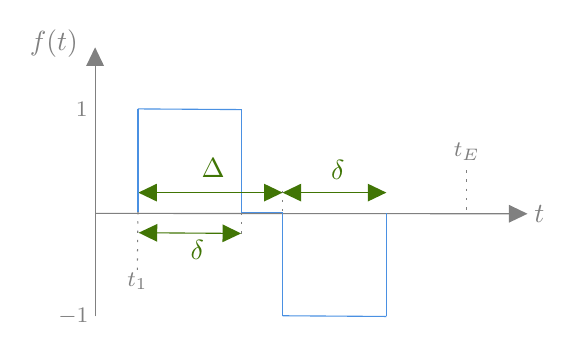
\begin{tikzpicture}[x=0.75pt,y=0.75pt,yscale=-1,xscale=1]
%uncomment if require: \path (0,300); %set diagram left start at 0, and has height of 300

%Straight Lines [id:da8882796881399757] 
\draw [color={rgb, 255:red, 128; green, 128; blue, 128 }  ,draw opacity=1 ]   (70.67,219.67) -- (70.67,93) ;
\draw [shift={(70.67,90)}, rotate = 90] [fill={rgb, 255:red, 128; green, 128; blue, 128 }  ,fill opacity=1 ][line width=0.08]  [draw opacity=0] (8.93,-4.29) -- (0,0) -- (8.93,4.29) -- cycle    ;
%Straight Lines [id:da664635011077519] 
\draw [color={rgb, 255:red, 128; green, 128; blue, 128 }  ,draw opacity=1 ]   (70.67,170) -- (276,170.2) ;
\draw [shift={(279,170.2)}, rotate = 180.06] [fill={rgb, 255:red, 128; green, 128; blue, 128 }  ,fill opacity=1 ][line width=0.08]  [draw opacity=0] (8.93,-4.29) -- (0,0) -- (8.93,4.29) -- cycle    ;
%Straight Lines [id:da17789798284277847] 
\draw [color={rgb, 255:red, 74; green, 144; blue, 226 }  ,draw opacity=1 ]   (91.33,119.67) -- (141.33,120) ;
%Straight Lines [id:da7626646796988461] 
\draw [color={rgb, 255:red, 74; green, 144; blue, 226 }  ,draw opacity=1 ]   (141.33,120) -- (141.33,169.67) ;
%Straight Lines [id:da4344394785262813] 
\draw [color={rgb, 255:red, 74; green, 144; blue, 226 }  ,draw opacity=1 ]   (141.33,169.67) -- (161,169.67) ;
%Straight Lines [id:da9282561195936812] 
\draw [color={rgb, 255:red, 74; green, 144; blue, 226 }  ,draw opacity=1 ]   (161,169.67) -- (161,219.33) ;
%Straight Lines [id:da08552867507313566] 
\draw [color={rgb, 255:red, 74; green, 144; blue, 226 }  ,draw opacity=1 ]   (161,219.33) -- (211,219.67) ;
%Straight Lines [id:da3575819731609853] 
\draw [color={rgb, 255:red, 74; green, 144; blue, 226 }  ,draw opacity=1 ]   (211,170) -- (211,219.67) ;
%Straight Lines [id:da12257132095246326] 
\draw [color={rgb, 255:red, 65; green, 117; blue, 5 }  ,draw opacity=1 ]   (94.67,179.35) -- (138,179.65) ;
\draw [shift={(141,179.67)}, rotate = 180.39] [fill={rgb, 255:red, 65; green, 117; blue, 5 }  ,fill opacity=1 ][line width=0.08]  [draw opacity=0] (8.93,-4.29) -- (0,0) -- (8.93,4.29) -- cycle    ;
\draw [shift={(91.67,179.33)}, rotate = 0.39] [fill={rgb, 255:red, 65; green, 117; blue, 5 }  ,fill opacity=1 ][line width=0.08]  [draw opacity=0] (8.93,-4.29) -- (0,0) -- (8.93,4.29) -- cycle    ;
%Straight Lines [id:da6443721529726347] 
\draw [color={rgb, 255:red, 65; green, 117; blue, 5 }  ,draw opacity=1 ]   (94.5,160) -- (158,160) ;
\draw [shift={(161,160)}, rotate = 180] [fill={rgb, 255:red, 65; green, 117; blue, 5 }  ,fill opacity=1 ][line width=0.08]  [draw opacity=0] (8.93,-4.29) -- (0,0) -- (8.93,4.29) -- cycle    ;
\draw [shift={(91.5,160)}, rotate = 0] [fill={rgb, 255:red, 65; green, 117; blue, 5 }  ,fill opacity=1 ][line width=0.08]  [draw opacity=0] (8.93,-4.29) -- (0,0) -- (8.93,4.29) -- cycle    ;
%Straight Lines [id:da43765182650583845] 
\draw [color={rgb, 255:red, 128; green, 128; blue, 128 }  ,draw opacity=1 ] [dash pattern={on 0.84pt off 2.51pt}]  (141.33,169.67) -- (141.33,180.33) ;
%Straight Lines [id:da9970970110276676] 
\draw [color={rgb, 255:red, 128; green, 128; blue, 128 }  ,draw opacity=1 ] [dash pattern={on 0.84pt off 2.51pt}]  (161,159) -- (161,169.67) ;
%Straight Lines [id:da9873905246267041] 
\draw [color={rgb, 255:red, 65; green, 117; blue, 5 }  ,draw opacity=1 ]   (164,160) -- (208,160) ;
\draw [shift={(211,160)}, rotate = 180] [fill={rgb, 255:red, 65; green, 117; blue, 5 }  ,fill opacity=1 ][line width=0.08]  [draw opacity=0] (8.93,-4.29) -- (0,0) -- (8.93,4.29) -- cycle    ;
\draw [shift={(161,160)}, rotate = 0] [fill={rgb, 255:red, 65; green, 117; blue, 5 }  ,fill opacity=1 ][line width=0.08]  [draw opacity=0] (8.93,-4.29) -- (0,0) -- (8.93,4.29) -- cycle    ;
%Straight Lines [id:da6590571773579443] 
\draw [color={rgb, 255:red, 128; green, 128; blue, 128 }  ,draw opacity=1 ] [dash pattern={on 0.84pt off 2.51pt}]  (249.73,149.2) -- (249.73,169.53) ;
%Straight Lines [id:da76362319772591] 
\draw [color={rgb, 255:red, 74; green, 144; blue, 226 }  ,draw opacity=1 ]   (91.33,119.67) -- (91.33,169.33) ;
%Straight Lines [id:da9036000522736403] 
\draw [color={rgb, 255:red, 128; green, 128; blue, 128 }  ,draw opacity=1 ] [dash pattern={on 0.84pt off 2.51pt}]  (91.33,169.33) -- (91,198.67) ;

% Text Node
\draw (63.6,88.2) node [anchor=east] [inner sep=0.75pt]  [color={rgb, 255:red, 128; green, 128; blue, 128 }  ,opacity=1 ]  {$f( t)$};
% Text Node
\draw (281,170.2) node [anchor=west] [inner sep=0.75pt]  [color={rgb, 255:red, 128; green, 128; blue, 128 }  ,opacity=1 ]  {$t$};
% Text Node
\draw (119.89,181.73) node [anchor=north] [inner sep=0.75pt]  [color={rgb, 255:red, 128; green, 128; blue, 128 }  ,opacity=1 ]  {$\textcolor[rgb]{0.25,0.46,0.02}{\delta }$};
% Text Node
\draw (127.55,142.4) node [anchor=north] [inner sep=0.75pt]  [color={rgb, 255:red, 128; green, 128; blue, 128 }  ,opacity=1 ]  {$\textcolor[rgb]{0.25,0.46,0.02}{\Delta }$};
% Text Node
\draw (187.55,154.99) node [anchor=south] [inner sep=0.75pt]  [color={rgb, 255:red, 128; green, 128; blue, 128 }  ,opacity=1 ]  {$\textcolor[rgb]{0.25,0.46,0.02}{\delta }$};
% Text Node
\draw (68.33,119.67) node [anchor=east] [inner sep=0.75pt]  [font=\footnotesize,color={rgb, 255:red, 128; green, 128; blue, 128 }  ,opacity=1 ]  {$1$};
% Text Node
\draw (68.67,219.67) node [anchor=east] [inner sep=0.75pt]  [font=\footnotesize,color={rgb, 255:red, 128; green, 128; blue, 128 }  ,opacity=1 ]  {$-1$};
% Text Node
\draw (91,197.4) node [anchor=north] [inner sep=0.75pt]  [font=\footnotesize,color={rgb, 255:red, 128; green, 128; blue, 128 }  ,opacity=1 ]  {$t_{1}$};
% Text Node
\draw (249.73,145.8) node [anchor=south] [inner sep=0.75pt]  [font=\footnotesize,color={rgb, 255:red, 128; green, 128; blue, 128 }  ,opacity=1 ]  {$t_{E}$};


\end{tikzpicture}

                \caption{}
                \label{fig:mri-gradient-profile:1}
            \end{subfigure}
            \hfill
            \begin{subfigure}{0.45\textwidth}
                

\tikzset{every picture/.style={line width=0.75pt}} %set default line width to 0.75pt        

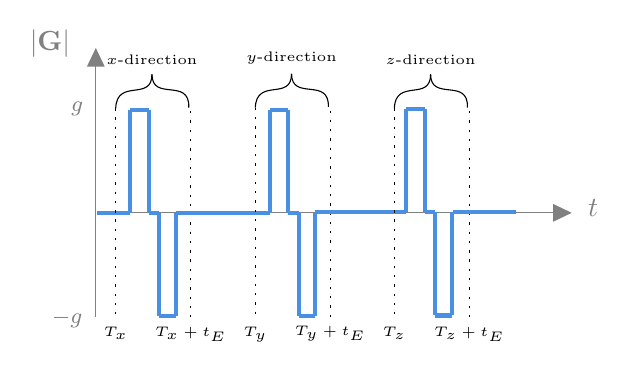
\begin{tikzpicture}[x=0.75pt,y=0.75pt,yscale=-1,xscale=1]
%uncomment if require: \path (0,300); %set diagram left start at 0, and has height of 300

%Straight Lines [id:da3774100901335702] 
\draw [color={rgb, 255:red, 128; green, 128; blue, 128 }  ,draw opacity=1 ]   (47.45,220) -- (47.45,93.33) ;
\draw [shift={(47.45,90.33)}, rotate = 90] [fill={rgb, 255:red, 128; green, 128; blue, 128 }  ,fill opacity=1 ][line width=0.08]  [draw opacity=0] (8.93,-4.29) -- (0,0) -- (8.93,4.29) -- cycle    ;
%Straight Lines [id:da9079908652045672] 
\draw [color={rgb, 255:red, 128; green, 128; blue, 128 }  ,draw opacity=1 ]   (48.07,169.75) -- (273.72,169.75) ;
\draw [shift={(276.72,169.75)}, rotate = 180] [fill={rgb, 255:red, 128; green, 128; blue, 128 }  ,fill opacity=1 ][line width=0.08]  [draw opacity=0] (8.93,-4.29) -- (0,0) -- (8.93,4.29) -- cycle    ;
%Straight Lines [id:da6473207409264472] 
\draw [color={rgb, 255:red, 74; green, 144; blue, 226 }  ,draw opacity=1 ][line width=1.5]    (64.04,120.08) -- (72.88,120.08) ;
%Straight Lines [id:da06919384086419744] 
\draw [color={rgb, 255:red, 74; green, 144; blue, 226 }  ,draw opacity=1 ][line width=1.5]    (72.88,120.08) -- (72.88,169.75) ;
%Straight Lines [id:da5657503776403818] 
\draw [color={rgb, 255:red, 74; green, 144; blue, 226 }  ,draw opacity=1 ][line width=1.5]    (72.88,169.75) -- (78.01,169.75) ;
%Straight Lines [id:da2035231243242186] 
\draw [color={rgb, 255:red, 74; green, 144; blue, 226 }  ,draw opacity=1 ][line width=1.5]    (78.01,169.75) -- (78.01,219.42) ;
%Straight Lines [id:da2770435671028688] 
\draw [color={rgb, 255:red, 74; green, 144; blue, 226 }  ,draw opacity=1 ][line width=1.5]    (78.01,219.42) -- (86,219.42) ;
%Straight Lines [id:da7146525103690513] 
\draw [color={rgb, 255:red, 74; green, 144; blue, 226 }  ,draw opacity=1 ][line width=1.5]    (86,169.75) -- (86,219.42) ;
%Straight Lines [id:da08072196166436374] 
\draw [color={rgb, 255:red, 74; green, 144; blue, 226 }  ,draw opacity=1 ][line width=1.5]    (64.04,120.08) -- (64.04,169.75) ;
%Straight Lines [id:da9026897276339403] 
\draw [color={rgb, 255:red, 74; green, 144; blue, 226 }  ,draw opacity=1 ][line width=1.5]    (48.07,169.75) -- (64.04,169.75) ;

%Straight Lines [id:da937386077900634] 
\draw  [dash pattern={on 0.84pt off 2.51pt}]  (93.13,120.75) -- (93.13,220.08) ;
%Curve Lines [id:da7511913583996024] 
\draw    (57.04,119.33) .. controls (57.61,104.67) and (74.5,116.33) .. (74.5,103) ;
%Curve Lines [id:da12325428458162424] 
\draw    (92.24,119) .. controls (92.8,104.33) and (74.5,116.33) .. (74.5,103) ;
%Straight Lines [id:da10398849489681083] 
\draw  [dash pattern={on 0.84pt off 2.51pt}]  (57.04,119.33) -- (57.04,220.25) ;
%Straight Lines [id:da08398923048196427] 
\draw [color={rgb, 255:red, 74; green, 144; blue, 226 }  ,draw opacity=1 ][line width=1.5]    (131.29,120.08) -- (140.13,120.08) ;
%Straight Lines [id:da32528202829910025] 
\draw [color={rgb, 255:red, 74; green, 144; blue, 226 }  ,draw opacity=1 ][line width=1.5]    (140.13,120.08) -- (140.13,169.75) ;
%Straight Lines [id:da8032661133457124] 
\draw [color={rgb, 255:red, 74; green, 144; blue, 226 }  ,draw opacity=1 ][line width=1.5]    (140.13,169.75) -- (145.26,169.75) ;
%Straight Lines [id:da3395149447265673] 
\draw [color={rgb, 255:red, 74; green, 144; blue, 226 }  ,draw opacity=1 ][line width=1.5]    (145.26,169.75) -- (145.26,219.42) ;
%Straight Lines [id:da6955133868719754] 
\draw [color={rgb, 255:red, 74; green, 144; blue, 226 }  ,draw opacity=1 ][line width=1.5]    (145.26,219.42) -- (153.25,219.42) ;
%Straight Lines [id:da011305796920654476] 
\draw [color={rgb, 255:red, 74; green, 144; blue, 226 }  ,draw opacity=1 ][line width=1.5]    (153.25,169.75) -- (153.25,219.42) ;
%Straight Lines [id:da4849350214011454] 
\draw [color={rgb, 255:red, 74; green, 144; blue, 226 }  ,draw opacity=1 ][line width=1.5]    (131.29,120.08) -- (131.29,169.75) ;
%Straight Lines [id:da5931104314922135] 
\draw [color={rgb, 255:red, 74; green, 144; blue, 226 }  ,draw opacity=1 ][line width=1.5]    (115.32,169.75) -- (131.29,169.75) ;

%Straight Lines [id:da8669231189933269] 
\draw  [dash pattern={on 0.84pt off 2.51pt}]  (160.38,120.5) -- (160.38,219.83) ;
%Curve Lines [id:da889044125391548] 
\draw    (124.29,119.08) .. controls (124.86,104.42) and (141.75,116.08) .. (141.75,102.75) ;
%Curve Lines [id:da9570400470225142] 
\draw    (159.49,118.75) .. controls (160.05,104.08) and (141.75,116.08) .. (141.75,102.75) ;
%Straight Lines [id:da32012167918494483] 
\draw  [dash pattern={on 0.84pt off 2.51pt}]  (124.29,119.08) -- (124.29,220) ;
%Straight Lines [id:da548151013698829] 
\draw [color={rgb, 255:red, 74; green, 144; blue, 226 }  ,draw opacity=1 ][line width=1.5]    (197.04,119.83) -- (205.88,119.83) ;
%Straight Lines [id:da7190010107515945] 
\draw [color={rgb, 255:red, 74; green, 144; blue, 226 }  ,draw opacity=1 ][line width=1.5]    (205.88,119.83) -- (205.88,169.5) ;
%Straight Lines [id:da5364622758177244] 
\draw [color={rgb, 255:red, 74; green, 144; blue, 226 }  ,draw opacity=1 ][line width=1.5]    (205.88,169.5) -- (211.01,169.5) ;
%Straight Lines [id:da22779131451799128] 
\draw [color={rgb, 255:red, 74; green, 144; blue, 226 }  ,draw opacity=1 ][line width=1.5]    (211.01,169.5) -- (211.01,219.17) ;
%Straight Lines [id:da946818978249186] 
\draw [color={rgb, 255:red, 74; green, 144; blue, 226 }  ,draw opacity=1 ][line width=1.5]    (211.01,219.17) -- (219,219.17) ;
%Straight Lines [id:da4540542047738241] 
\draw [color={rgb, 255:red, 74; green, 144; blue, 226 }  ,draw opacity=1 ][line width=1.5]    (219,169.5) -- (219,219.17) ;
%Straight Lines [id:da47688281363458307] 
\draw [color={rgb, 255:red, 74; green, 144; blue, 226 }  ,draw opacity=1 ][line width=1.5]    (197.04,119.83) -- (197.04,169.5) ;
%Straight Lines [id:da15791990154946056] 
\draw [color={rgb, 255:red, 74; green, 144; blue, 226 }  ,draw opacity=1 ][line width=1.5]    (181.07,169.5) -- (197.04,169.5) ;

%Straight Lines [id:da21285085567206097] 
\draw  [dash pattern={on 0.84pt off 2.51pt}]  (227.38,120.75) -- (227.38,220.08) ;
%Curve Lines [id:da4611087330179324] 
\draw    (191.29,119.33) .. controls (191.86,104.67) and (208.75,116.33) .. (208.75,103) ;
%Curve Lines [id:da5611948742808552] 
\draw    (226.49,119) .. controls (227.05,104.33) and (208.75,116.33) .. (208.75,103) ;
%Straight Lines [id:da7247349322588634] 
\draw  [dash pattern={on 0.84pt off 2.51pt}]  (191.29,119.33) -- (191.29,220.25) ;
%Straight Lines [id:da47838174999972116] 
\draw [color={rgb, 255:red, 74; green, 144; blue, 226 }  ,draw opacity=1 ][line width=1.5]    (86,169.75) -- (115.32,169.75) ;
%Straight Lines [id:da561199135094695] 
\draw [color={rgb, 255:red, 74; green, 144; blue, 226 }  ,draw opacity=1 ][line width=1.5]    (153.25,169.5) -- (183.25,169.5) ;
%Straight Lines [id:da23861894222113644] 
\draw [color={rgb, 255:red, 74; green, 144; blue, 226 }  ,draw opacity=1 ][line width=1.5]    (219.5,169.25) -- (249.75,169.25) ;

% Text Node
\draw (36.35,88.2) node [anchor=east] [inner sep=0.75pt]  [color={rgb, 255:red, 128; green, 128; blue, 128 }  ,opacity=1 ]  {$|\mathbf{G} |$};
% Text Node
\draw (283.36,167.53) node [anchor=west] [inner sep=0.75pt]  [color={rgb, 255:red, 128; green, 128; blue, 128 }  ,opacity=1 ]  {$t$};
% Text Node
\draw (42.54,119.67) node [anchor=east] [inner sep=0.75pt]  [font=\footnotesize,color={rgb, 255:red, 128; green, 128; blue, 128 }  ,opacity=1 ]  {$g$};
% Text Node
\draw (42.21,220.67) node [anchor=east] [inner sep=0.75pt]  [font=\footnotesize,color={rgb, 255:red, 128; green, 128; blue, 128 }  ,opacity=1 ]  {$-g$};
% Text Node
\draw (74.5,99.6) node [anchor=south] [inner sep=0.75pt]  [font=\tiny]  {$x\text{\mbox{-}direction}$};
% Text Node
\draw (57.04,223.65) node [anchor=north] [inner sep=0.75pt]  [font=\tiny]  {$T_{x}$};
% Text Node
\draw (93.13,223.48) node [anchor=north] [inner sep=0.75pt]  [font=\tiny]  {$T_{x} +t_{E}$};
% Text Node
\draw (141.75,99.35) node [anchor=south] [inner sep=0.75pt]  [font=\tiny]  {$y\text{\mbox{-}direction}$};
% Text Node
\draw (124.29,223.4) node [anchor=north] [inner sep=0.75pt]  [font=\tiny]  {$T_{y}$};
% Text Node
\draw (160.38,223.23) node [anchor=north] [inner sep=0.75pt]  [font=\tiny]  {$T_{y} +t_{E}$};
% Text Node
\draw (208.75,99.6) node [anchor=south] [inner sep=0.75pt]  [font=\tiny]  {$z\text{\mbox{-}direction}$};
% Text Node
\draw (191.29,223.65) node [anchor=north] [inner sep=0.75pt]  [font=\tiny]  {$T_{z}$};
% Text Node
\draw (227.38,223.48) node [anchor=north] [inner sep=0.75pt]  [font=\tiny]  {$T_{z} +t_{E}$};


\end{tikzpicture}

                \caption{}
                \label{fig:mri-gradient-profile:3}
            \end{subfigure}
            \caption{(a) Sketch of the time profile given in Equation \eqref{eq:time-profile} between $t=0$ and $t=t_E$. (b) Magnetic gradients applied sequentially in the 3 coordinate directions, for which the magnitude of the magnetic gradients is illustrated here. For each sequence, the spin is initialised $\phi = 0$ at $t = T_x, T_y, T_z$, and measurements are taken at $t = T_x + t_\text{E}$, $t = T_y + t_\text{E}$, and $t = T_z + t_\text{E}$.}
            \label{fig:mri-gradient-profile}
        \end{figure}
    
        The so-called $b$-value parameterises the magnetic gradient strength, related to $\vec{G}(t)$ through the following \cite{bernsteinHandbookMRIPulse2004}:
        \begin{equation}
            b = (2\gamma)^2 \int_0^{t_E} \norm{\vec{k}(t)}^2 \diff t,
        \end{equation}
        where $\vec{k}$ is defined by
        \begin{equation}
            \vec{k}(t) = \frac{\gamma^2}{2\pi} \int_0^t \vec{G}(s) \diff s,
        \end{equation}
        and $\gamma$ is the gyromagnetic ratio \cite{bernsteinHandbookMRIPulse2004}, fixed as $\gamma = 42.57 \times 2\pi \times 10^6$~\unit{\radian\per\second\per\tesla} for our application \cite{dellschaftHaemodynamicsHumanPlacenta2020}. Using Equations \eqref{eq:time-profile} and \eqref{eq:g}, \citeauthor{lebihanDiffusionPerfusionMagnetic1995} \cite{lebihanDiffusionPerfusionMagnetic1995} states that this relation may be simplified to
        \begin{equation}
            b = \gamma^2 g^2 \delta^2 (\Delta - \delta/3),
            \label{eq:g-to-b}
        \end{equation}
        where we assume that the sequences are non-overlapping (i.e., $T_x + t_E < T_y$ and $T_y + t_E < T_z$).
    
        An isochromat is an ensemble of individual particles on a scale smaller than voxels, whose individual magnetic spins $\phi$ are assumed to evolve in the same way \cite{jungSpinEchoMagnetic2013}. Depending upon the strength of the magnetic field at an isochromat's location, the magnetic spin may evolve differently. The evolution of the $j$th isochromat's spin is given by
        \begin{equation}
            \phi_j(t) = \gamma \int_0^t \vec{G}(\tau) \cdot \vec{r}_j(\tau) \diff \tau,
            \label{eq:phi}
        \end{equation}
        where $\vec{r}_j$ is the displacement of the $j$th isochromat, given as $\vec{r}_j(t) = \vec{x}_j(t) - \vec{x}_j(0)$, and $\vec{x}_j(t)$ is the position of the $j$th isochromat at time $t$ (see \cite{bernsteinHandbookMRIPulse2004}). We note here that this corresponds to integrating the Bloch-Torrey equation in Equation \eqref{eq:bloch-torrey} with $\vec{D} = \vec{0}$ (i.e., the Bloch equation \cite{bernsteinHandbookMRIPulse2004}); this simplification is made due to the stronger effects of so-called pseudo-diffusion present in studies of blood flow \cite{torreyBlochEquationsDiffusion1956,lebihanWhatCanWe2019}.
        
        The MRI signal itself is measured at the echo time, $t_E$. For a magnetic gradient applied only in one axis direction, the complex nuclear magnetisation at time $t$ for the $j$th isochromat is given by \cite{bernsteinHandbookMRIPulse2004} to be
        \begin{equation}
            M_j(t) := e^{-\iu\phi_j(t)}.
        \end{equation}
        The total nuclear magnetisation in a voxel at time $t$ is then given by 
        \begin{equation}
            \bar{M}(t) := \sum^{N_x}_{j=1} M_j(t),
            \label{eq:nuclear-magnetisation}
        \end{equation}
        and the corresponding signal at the echo time is given by
        \begin{equation}
            S_x := \left| \bar{M}(T_x + t_\text{E}) \right|,
            \label{eq:signal-x}
        \end{equation}
        where the sum is over all $N_x$ isochromats in a given voxel. Similar expressions follow for $S_y$ and $S_z$; for clarity, we have
        \begin{equation}
            S_y := \left| \bar{M}(T_y + t_\text{E}) \right|,
        \end{equation}
        \begin{equation}
            S_z := \left| \bar{M}(T_z + t_\text{E}) \right|.
        \end{equation}
        The total signal in a given voxel is then computed as 
        \begin{equation}
            S := S_x + S_y + S_z.
            \label{eq:total-s}
        \end{equation}

        Our approach here focusses on motion-sensitising MRI, where the dependence of $S$ upon $b$ can help reveal flow characteristics. We will now introduce an algorithm for computing $S$ for a given $b$, where particles are advected by an underlying velocity field.

    \section{Algorithm for computing numerical MRI signals} \label{sec:numerical-mri:algorithm}
        For all the simulations presented throughout the remainder of Chapter \ref{sec:numerical-mri}, we take voxels of size \qtyproduct{2.5x2.5}{\milli\metre} spanning the entire domain of interest. We then distribute the initial positions of many isochromats such that there are $20 \times 20$ equally-spaced isochromats in each voxel, where the $j$th isochromat's initial position is denoted by $\vec{x}^0_j$. Given the initial positions of each isochromat, we evolve the position of each isochromat according to the following:
        \begin{equation}
            \vec{x}^{n+1}_j = \vec{x}^n_j + \vec{u}(\vec{x}^0_j) ~ \Delta t,
        \end{equation}
        for time points $t^n$ between $t=0$ and $t=t_E$: $\{ t^n := n \Delta t \mid 0 \leq n \leq N_t \}$. Note that we fix $\vec{u}$ at $t = 0$ for computational simplicity. We discretise spin evolution from Equation \eqref{eq:phi} in a similar way:
        \begin{equation}
            \phi^{n+1}_j = \phi^n_j + \gamma \, \vec{G}(T_d + t^{n+1}) \cdot (\vec{x}^{n+1}_j - \vec{x}^0_j) ~ \Delta t,
        \end{equation}
        where $T_d$ is replaced by one of $T_x, T_y, T_z$ depending upon the coordinate direction in which the spins are being measured.
        
        Algorithm \ref{alg:mri} gives the general algorithm for computing $S$, which is calculated over every voxel and many choices of $b$. In specific terms for our application, we start by selecting the set of isochromat positions that lie in the given voxel. We next obtain a steady-state velocity field; \S\ref{sec:numerical-mri:manufactured} will use some simple manufactured flow fields, whereas \S\ref{sec:numerical-mri:placental} will use a placental velocity field obtained from Chapters \ref{sec:modelling} and \ref{sec:numerical-methods}. For each $b$, we calculate $\vec{G}(t)$ given in Equation \eqref{eq:g}, where $g$ is calculated through Equation \eqref{eq:g-to-b}, and $b$ is chosen as $5001$ equally-spaced values between $b=\qty{0}{\second\per\milli\metre^2}$ and $b=\qty{500}{\second\per\milli\metre^2}$. For simplicity, we take $531$ equally-spaced time points between $t=0$ and $t = t_E \equiv \qty{53}{\milli\second}$. In each voxel, a value of $S$ is computed for every value of $b$; calculations for each $S$ can therefore be done independently, which allows for easy parallel execution if desired. We note that this procedure may advect isochromats outside the voxel in which they are being measured; this isn't significant due to the short timescales and slow velocities involved. 
        
        \begin{algorithm}
            \SetKwInOut{Input}{input}
            \SetKwInOut{Output}{output}
            \Input{$\{\bar{\vec{x}}_j\}$: Set of sampled initial positions for each of the $N_x$ isochromats. \\
                   $\vec{u}(\vec{x})$: Steady velocity field. \\
                   $\vec{G}(t)$: Gradient sequence for a particular field strength, $b$. \\
                   $\{t^n\}$: Set of $N_t$ time-steps, each separated by $\Delta t$. \\
            }
            \ForEach{$d \in \{ \mlq x \mrq, \mlq y \mrq, \mlq z \mrq \}$ (dimension)}{
                Initialise spins for all isochromats: $\{ \phi_j^0 \} \gets \{0\}$ \\
                Initialise positions for all isochromats: $\{ \vec{x}_j^0 \} \gets \{\bar{\vec{x}}_j\}$ \\
                \For{$n = 0$ \KwTo $N_t - 1$ (time-steps)}{
                    \For{$j = 1$ \KwTo $N_x$ (isochromats)}{
                        $\vec{x}_j^{n+1} \gets \vec{x}_j^n + \vec{u}(\vec{x}_j^0) ~ \Delta t$ \\
                        $\phi_j^{n+1} \gets \phi_j^n + \gamma ~ \vec{G}(T_d + t^{n+1}) \cdot (\vec{x}_j^{n+1} - \vec{x}_j^0) ~ \Delta t$
                    } 
                } 
                $S_d \gets \left| \sum_{j=1}^{N_x} \exp \left( -\iu \phi_j^{N_t} \right) \right|$
            } 
            $S \gets S_x + S_y + S_z$ \\
            \Output{$S$}
            \caption{Numerically generates a signal $S$, given: a set of initial positions for each isochromat, a steady-state velocity field, a gradient sequence, and a set of discretised time points. This algorithm is used in each voxel for every choice of $b$.}
            \label{alg:mri}
        \end{algorithm}

        We will now use some simple manufactured flows to understand the dependence of MRI signal ($S$) upon magnetic field strength ($b$) through $S$-vs-$b$ graphs. Graphs such as these are useful to study, as different patterns can provide insight into the underlying sub-voxel flow field.

    \section{MRI for simple manufactured flows} \label{sec:numerical-mri:manufactured}
        Here, we will present a series of carefully designed example cases aimed at understanding the behaviour of MRI signals over different 2D velocity fields. For simplicity, each example is defined on the domain $\Omega := [0, 1]^2 \unit{\metre^2}$, with a single voxel spanning the entire domain. We choose $5001$ equally-spaced $b$-values ranging \qtyrange{0}{500}{\second\per\milli\meter^2}, with a $20\times20$ grid of isochromats that are initially equally-spaced over $\Omega$. Some of these examples will then be referred to when discussing the results of \S\ref{sec:numerical-mri:placental}.

        \subsection{Shear flow} \label{sec:numerical-mri:manufactured:shear}
            In the following three examples, we have a velocity field describing shear flow, given by
            \begin{equation}
                \vec{u}(\vec{x}) =
                \begin{cases}
                    U_1 ~ \vec{\hat{y}} & \text{if } x < 0.5, \\
                    U_2 ~ \vec{\hat{y}} & \text{if } x \geq 0.5,
                \end{cases}
            \end{equation}
            where $U_1$ and $U_2$ are scaling constants, and $\vec{\hat{y}}$ is the unit normal vector in the $y$-direction. The following subsubsections consider three different choices of $U_1$ and $U_2$ and the effect these have on $S$.

            \subsubsection{Example 1} \label{sec:numerical-mri:manufactured:shear:1}
                We initially select $U_1 = \qty{0.005}{\metre\per\second}$ and $U_2 = \qty{0.01}{\metre\per\second}$. This velocity field is visualised in Figure \ref{fig:mri-shear-1:quiver}.

                We denote $S$, $S_x$, and $S_y$ at $b=0$ respectively by $S_0$, $S_{x,0}$, and $S_{y,0}$, and denote the normalised signals by
                \begin{subequations}
                    \begin{align}
                        \bar{S} & := S/S_0, \\
                        \bar{S}_x & := S_x/S_{x,0}, \\
                        \bar{S}_y & := S_y/S_{y,0}.
                    \end{align}
                \end{subequations}
                We note that $S = S_x + S_y$ here, since there is no $z$-component to the signal in the 2D simulations presented in this thesis; we also note that $\bar{S}, \bar{S}_x, \bar{S}_y \in [0, 1]$. Figure \ref{fig:mri-shear-1:s-vs-b} presents these normalised signals against $b$, where we see that $\bar{S}$ oscillates between $0.5$ and $1$, with a decreasing frequency as $b$ increases.

                To understand why the oscillations are confined between $0.5$ and $1$, let's consider Equation \eqref{eq:total-s}, which states that the total signal $S$ for this 2D example is composed of signals from both the $x$- and $y$-directions (for simplicity, we set $S_z \equiv 0$ for the 2D flows in this thesis). The blue and green lines in Figure \ref{fig:mri-shear-1:s-vs-b} respectively show the $x$- and $y$-components of the normalised signal ($\bar{S}_x$ and $\bar{S}_y$) plotted against $b$. In the case of this artificially-created 2D velocity field, there is no movement in the $x$-direction, and therefore isochromats experience no variation in magnetic field strength, consequently giving no signal loss for $S_x$ (i.e, $S_x \equiv 1$). We note that full signal will always be retained at $b=0$ ($\bar{S}_{x,0} = 1$ and $\bar{S}_{y,0} = 1$), and in the most extreme case $\bar{S}_y$ will lose all signal ($\bar{S}_y = 0$) for some $b > 0$. This therefore gives $\bar{S} = 1$ when $\bar{S}_y = 1$, and $\bar{S} = 0.5$ when $\bar{S}_y = 0$.
                
                To understand the frequency decrease, we recall Equation \eqref{eq:phi}, which shows that $\phi$ depends upon the integral of $\vec{G}$; in turn, Equation \eqref{eq:g-to-b} indicates that $b$ depends quadratically on $g$, meaning that the frequency decrease is quadratic in $b$. Figure \ref{fig:mri-shear-1:s-vs-g} instead plots $S$ against $g$, for which we see that the frequency is constant for increasing $g$.
                
                Figure \ref{fig:mri-shear-1:s-vs-b} shows that $\bar{S}_y$ oscillates between $0$ and $1$, and at minima the derivative is discontinuous. This effect where signal is recovered quickly from $S=0$ is sometimes known as a \textit{rebound} or \textit{rebounding}. The non-unity values of $\bar{S}_y$ can be explained by visualising the nuclear magnetisation using Equation \eqref{eq:nuclear-magnetisation}. Figure \ref{fig:mri-shear-1:b} shows the different values of $\bar{M}(T_y + t_E)$ for different choices of $b$, where the colour of the arrow varies from lightest green ($b=\qty{0}{\second\per\milli\metre^2}$) to darkest green ($b=\qty{2}{\second\per\milli\metre^2}$); we choose to only visualise $\bar{M}(T_y + t_E)$ here because there is no signal loss for $\bar{M}(T_x + t_E)$; this shows how $S_y$ decreases with increasing $b$ in this range. Although not illustrated, at approximately $b=\qty{10.5}{\second\per\milli\metre^2}$, the magnitude of $\bar{M}(T_y + t_E)$ (i.e., $S_y$) is approximately zero, giving a minimum in Figure \ref{fig:mri-shear-1:s-vs-b}, for which the derivative is discontinuous as $\bar{M}(T_y + t_E)$ passes through the origin.
                
                We recall from Equation \eqref{eq:nuclear-magnetisation} that $\bar{M}(T_y + t_E)$ is computed from the sum of several unit magnitude complex numbers which encode the spins for each individual isochromat; Figure \ref{fig:mri-shear-1:spins} visualises the set of all isochromats in the voxel for $b=\qty{2}{\second\per\milli\metre^2}$ denoted by $\{ M_j(T_y + t_E) \}$, with $\bar{M}(T_y + t_E)$ also shown. We highlight that the most important feature of this test case is that the isochromats are clustered into two groups, corresponding to the two choices of fluid speed on either side of the domain; this is due to Equation \eqref{eq:phi} and the dependence of spin $\phi$ upon the displacement $\vec{r}$, which will accumulate at one of two rates.

                \begin{figure}
                    \thisfloatpagestyle{empty}
                    %% SHEAR TEST (SPLIT)
                    %   Generated and plotted from test 1 in ./drivers/mri_tests.py.
                    %   Implicitly calls plot_quiver() in ./plotting/plot_mri_spins.py
                    \begin{subfigure}{0.5\textwidth}
                        \centering
                        \includegraphics[width=\textwidth]{diagrams/results-mri/simple-tests/mri-spins_quiver_2D_shear_test_1.png}
                        \caption{}
                        \label{fig:mri-shear-1:quiver}
                    \end{subfigure}
                    \\
                    \begin{subfigure}{0.4\textwidth}
                        \centering
                        \includegraphics[width=\textwidth]{diagrams/results-mri/simple-tests/mri-spins_sall-vs-b_2D_shear_test_1.png}
                        \caption{}
                        \label{fig:mri-shear-1:s-vs-b}
                    \end{subfigure}
                    \vspace{4mm} % Weird place, I know, but this is the only place that gave spacing between the 2nd and 3rd rows.
                    \begin{subfigure}{0.4\textwidth}
                        \centering
                        \includegraphics[width=\textwidth]{diagrams/results-mri/simple-tests/mri-spins_gall-vs-b_2D_shear_test_1.png}
                        \caption{}
                        \label{fig:mri-shear-1:s-vs-g}
                    \end{subfigure}
                    \begin{subfigure}{0.4\textwidth}
                        \centering
                        \includegraphics[width=\textwidth]{diagrams/results-mri/simple-tests/mri-spins_b_2D_shear_test_1.png}
                        \caption{}
                        \label{fig:mri-shear-1:b}
                    \end{subfigure}
                    \begin{subfigure}{0.4\textwidth}
                        \centering
                        \includegraphics[width=\textwidth]{diagrams/results-mri/simple-tests/mri-spins_avg_2D_shear_test_1.png}
                        \caption{}
                        \label{fig:mri-shear-1:spins}
                    \end{subfigure}
                    \caption{The shear flow example from \S\ref{sec:numerical-mri:manufactured:shear:1} with $U_1 = \qty{0.005}{\metre\per\second}$ and $U_2 = \qty{0.01}{\metre\per\second}$, showing visualisations of (a) the velocity field for each isochromat, (b) $S$ against $b$, (c) $S$ against $g$, (d) $\bar{M}(T_y + t_E)$ for different choices of $b$, and (e) individual isochromat values of $\{ M_j(T_y + t_E) \}$ for $b=\qty{2}{\second\per\milli\metre^2}$.}
                    \label{fig:mri-shear-1}
                \end{figure}

            \subsubsection{Example 2} \label{sec:numerical-mri:manufactured:shear:2}
                We will now give another example of a shear flow velocity field, which is visualised in Figure \ref{fig:mri-shear-2:quiver}, this time with $U_1 = \qty{0.0025}{\metre\per\second}$ and $U_2 = \qty{-0.0025}{\metre\per\second}$. Figure \ref{fig:mri-shear-2:s-vs-b} shows the $S$-vs-$b$ graph for this example. Interestingly, this graph is identical to the one shown in Figure \ref{fig:mri-shear-1:s-vs-b}. Figure \ref{fig:mri-shear-2:b} shows the values of $\bar{M}(T_y + t_E)$ from $b=\qty{0}{\second\per\milli\metre^2}$ (lightest green) to $b=\qty{2}{\second\per\milli\metre^2}$ (darkest green), which shows that the argument of the complex number $\bar{M}(T_y + t_E)$ (i.e., $\phi$) is unchanging, whilst the magnitude of $\bar{M}(T_y + t_E)$ (i.e., $S$) does change --- and does so in precisely the same way as the previous example. Lastly, Figure \ref{fig:mri-shear-2:spins} shows each individual isochromat's spin for $b = \qty{2}{\second\per\milli\metre^2}$, which are again clustered into two groups that are separated by the same phase as the previous example.
                
                Crucially, this second test is an example of the non-uniqueness of MRI signals when measuring two different flow fields; the important message here is that is it the difference in \text{relative} speed between the groups that causes gives the behaviour in $S$: since the difference between the two velocity scalings are equal in both examples ($|U_2 - U_1| = \qty{0.005}{\metre\per\second}$), they exhibit exactly the same signal curve against $b$. This is shown succinctly by Equation \eqref{eq:phi}, which shows that the evolution of $\phi$ depends upon the displacement of the isochromats, each of which displace with velocity $\vec{u}(\vec{x}^0)$.

                \begin{figure}
                    %% SHEAR TEST (OPPOSING DIRECTIONS)
                    %   Generated and plotted from test 2 in ./drivers/mri_tests.py.
                    %   Implicitly calls plot_quiver() in ./plotting/plot_mri_spins.py
                    \begin{subfigure}{0.4\textwidth}
                        \centering
                        \includegraphics[width=\textwidth]{diagrams/results-mri/simple-tests/mri-spins_quiver_2D_shear_test_2.png}
                        \caption{}
                        \label{fig:mri-shear-2:quiver}
                    \end{subfigure}
                    \vspace{4mm} % Weird place, I know, but this is the only place that gave spacing between the 1st and 2nd rows.
                    \begin{subfigure}{0.4\textwidth}
                        \centering
                        \includegraphics[width=\textwidth]{diagrams/results-mri/simple-tests/mri-spins_sall-vs-b_2D_shear_test_2.png}
                        \caption{}
                        \label{fig:mri-shear-2:s-vs-b}
                    \end{subfigure}
                    \begin{subfigure}{0.4\textwidth}
                        \centering
                        \includegraphics[width=\textwidth]{diagrams/results-mri/simple-tests/mri-spins_b_2D_shear_test_2.png}
                        \caption{}
                        \label{fig:mri-shear-2:b}
                    \end{subfigure}
                    \begin{subfigure}{0.4\textwidth}
                        \centering
                        \includegraphics[width=\textwidth]{diagrams/results-mri/simple-tests/mri-spins_avg_2D_shear_test_2.png}
                        \caption{}
                        \label{fig:mri-shear-2:spins}
                    \end{subfigure}
                    \caption{The shear flow example from \S\ref{sec:numerical-mri:manufactured:shear:2} with $U_1 = \qty{0.0025}{\metre\per\second}$ and $U_2 = \qty{-0.0025}{\metre\per\second}$, showing visualisations of (a) the velocity field for each isochromat, (b) $S$ against $b$, (c) $\bar{M}(T_y + t_E)$ for different choices of $b$, and (d) individual isochromat values of $\{ M_j(T_y + t_E) \}$ for $b=\qty{2}{\second\per\milli\metre^2}$.}
                    \label{fig:mri-shear-2}
                \end{figure}

            \subsubsection{Example 3} \label{sec:numerical-mri:manufactured:shear:3}
                One final example of shear flow is to take $U_1 = \qty{0.01}{\metre\per\second}$ and $U_2 = \qty{0.01}{\metre\per\second}$, which we note gives a constant flow. This velocity field is visualised in Figure \ref{fig:mri-shear-3:quiver}. The $S$-vs-$b$ graph is shown in Figure \ref{fig:mri-shear-3:s-vs-b}, which attains full signal for all choices of $b$. Because $U_2 - U_1 = 0$ here, Figure \ref{fig:mri-shear-3:spins} shows that there is no signal loss for all $b$. Although Figure \ref{fig:mri-shear-3:b} shows the angle of $\bar{M}(T_y + t_E)$ changing for different $b$, all the isochromats remain in a single group, therefore giving $\bar{S}=1$.
    
                \begin{figure}
                    %% SHEAR TEST (UNIFORM)
                    %   Generated and plotted from test 3 in ./drivers/mri_tests.py.
                    %   Implicitly calls plot_quiver() in ./plotting/plot_mri_spins.py
                    \begin{subfigure}{0.4\textwidth}
                        \centering
                        \includegraphics[width=\textwidth]{diagrams/results-mri/simple-tests/mri-spins_quiver_2D_shear_test_3.png}
                        \caption{}
                        \label{fig:mri-shear-3:quiver}
                    \end{subfigure}
                    \vspace{4mm} % Weird place, I know, but this is the only place that gave spacing between the 1st and 2nd rows.
                    \begin{subfigure}{0.4\textwidth}
                        \centering
                        \includegraphics[width=\textwidth]{diagrams/results-mri/simple-tests/mri-spins_sall-vs-b_2D_shear_test_3.png}
                        \caption{}
                        \label{fig:mri-shear-3:s-vs-b}
                    \end{subfigure}
                    \begin{subfigure}{0.4\textwidth}
                        \centering
                        \includegraphics[width=\textwidth]{diagrams/results-mri/simple-tests/mri-spins_b_2D_shear_test_3.png}
                        \caption{}
                        \label{fig:mri-shear-3:b}
                    \end{subfigure}
                    \begin{subfigure}{0.4\textwidth}
                        \centering
                        \includegraphics[width=\textwidth]{diagrams/results-mri/simple-tests/mri-spins_avg_2D_shear_test_3.png}
                        \caption{}
                        \label{fig:mri-shear-3:spins}
                    \end{subfigure}
                    \caption{The shear flow example from \S\ref{sec:numerical-mri:manufactured:shear:3} with $U_1 = \qty{0.01}{\metre\per\second}$ and $U_2 = \qty{0.01}{\metre\per\second}$, showing a visualisation of (a) the velocity field for each isochromat, (b) $S$ against $b$, (c) $\bar{M}(T_y + t_E)$ for different choices of $b$, and (d) individual isochromat values of $\{ M_j(T_y + t_E) \}$ for $b=\qty{2}{\second\per\milli\metre^2}$.}
                    \label{fig:mri-shear-3}
                \end{figure}

        \subsection{Rotational flow} \label{sec:numerical-mri:manufactured:rotational}
            For the next example of velocity field, we introduce a rotational flow, given by
            \begin{equation}
                \vec{u}(x, y) = \begin{pmatrix}-U_1 y / L \\ U_2 x / L\end{pmatrix},
            \end{equation}
            where $L = \qty{1}{\metre}$ is the length of the domain.
            For simplicity, we select $U_1 = \qty{0.01}{\metre\per\second}$ and $U_2 = \qty{0.01}{\metre\per\second}$, which gives the velocity field illustrated in Figure \ref{fig:mri-rotational:quiver}.
            
            The $S$-vs-$b$ graph is shown in Figure \ref{fig:mri-rotational:s-vs-b}; similar to the previous examples, we observe oscillations with decreasing frequency as $b$ increases (or equivalently constant frequency as $g$ increases). Figure \ref{fig:mri-rotational:b} also shows a familiar pattern for each $b$ to those shown in the shear flow examples. Figure \ref{fig:mri-rotational:spins} plots the individual spins for each isochromat for $b=\qty{2}{\second\per\milli\metre^2}$, which, unlike the previous examples, cluster into $20$ values associated with the number of isochromats lying in the $y$-direction. $b=\qty{9.4}{\second\per\milli\metre^2}$ corresponds to the first local minimum of $\bar{S} \approx 0$ in Figure \ref{fig:mri-rotational:s-vs-b}, which is where the isochromats become equally-separated and therefore give a signal of $\bar{S}=0$. Figure \ref{fig:mri-rotational:spins_min} shows the individual spins distributed equally for $b=\qty{9.4}{\second\per\milli\metre^2}$.
            
            We note that the amplitude of the oscillations decreases as $b$ increases in Figure \ref{fig:mri-rotational:s-vs-b}. In previous examples, full signal ($\bar{S}=1$) was regained through an effect known as \textit{refocusing} --- where spins coincide at $b>0$. Refocusing does not happen to the same extent here due to the spins clustering into $20$ values (due to the number of sample points), rather than just $2$. For $b = \qty{19.3}{\second\per\milli\metre^2}$, Figure \ref{fig:mri-rotational:s-vs-b} shows a local maximum of $\bar{S} \approx 0.22$. Figure \ref{fig:mri-rotational:spins_max} plots the individual spins again for this choice of $b$, which shows $14$ different phases in which isochromats cluster into, with $6$ of those phases in the lower right showing two isochromats overlapping (indicated by the darker gray arrow opacity). The lowering amplitude of $\bar{S}$ is therefore due to a weakening refocussing effect, where fewer isochromats overlap with the same phase, resulting in a gradually smaller value of $\bar{S}$.

            \begin{figure}
                %% ROTATIONAL TEST
                %   Generated and plotted from test 4 in ./drivers/mri_tests.py.
                %   Implicitly calls plot_quiver() in ./plotting/plot_mri_spins.py
                \begin{subfigure}{0.4\textwidth}
                    \centering
                    \includegraphics[width=\textwidth]{diagrams/results-mri/simple-tests/mri-spins_quiver_2D_rotational_test_4.png}
                    \caption{}
                    \label{fig:mri-rotational:quiver}
                \end{subfigure}
                \vspace{4mm} % Weird place, I know, but this is the only place that gave spacing between the 1st and 2nd rows.
                \begin{subfigure}{0.4\textwidth}
                    \centering
                    \includegraphics[width=\textwidth]{diagrams/results-mri/simple-tests/mri-spins_sall-vs-b_2D_rotational_test_4.png}
                    \caption{}
                    \label{fig:mri-rotational:s-vs-b}
                \end{subfigure}
                \begin{subfigure}{0.4\textwidth}
                    \centering
                    \includegraphics[width=\textwidth]{diagrams/results-mri/simple-tests/mri-spins_b_2D_rotational_test_4.png}
                    \caption{}
                    \label{fig:mri-rotational:b}
                \end{subfigure}
                \begin{subfigure}{0.4\textwidth}
                    \centering
                    \includegraphics[width=\textwidth]{diagrams/results-mri/simple-tests/mri-spins_avg_2D_rotational_test_4.png}
                    \caption{}
                    \label{fig:mri-rotational:spins}
                \end{subfigure}
                \begin{subfigure}{0.4\textwidth}
                    \centering
                    \includegraphics[width=\textwidth]{diagrams/results-mri/simple-tests/mri-spins_avg_2D_rotational_test_4_b9.4.png}
                    \caption{}
                    \label{fig:mri-rotational:spins_min}
                \end{subfigure}
                \begin{subfigure}{0.4\textwidth}
                    \centering
                    \includegraphics[width=\textwidth]{diagrams/results-mri/simple-tests/mri-spins_avg_2D_rotational_test_4_b19.3.png}
                    \caption{}
                    \label{fig:mri-rotational:spins_max}
                \end{subfigure}
                \caption{The rotational flow example from \S\ref{sec:numerical-mri:manufactured:rotational} with $U_1 = \qty{0.01}{\metre\per\second}$ and $U_2 = \qty{0.01}{\metre\per\second}$, showing visualisations of (a) the velocity field for each isochromat, (b) $S$ against $b$, and (c) $\bar{M}(T_y + t_E)$ for different choices of $b$. (d), (e), and (f) respectively show individual isochromat values of $\{ M_j(T_y + t_E) \}$ for $b=\qty{2}{\second\per\milli\metre^2}$, $b=\qty{9.4}{\second\per\milli\metre^2}$, and $b=\qty{19.3}{\second\per\milli\metre^2}$.}
                \label{fig:mri-rotational}
            \end{figure}

            % \begin{figure}
            %     \begin{subfigure}[b]{0.3\textwidth}
            %         \centering
            %         \includegraphics[width=\textwidth]{diagrams/results-mri/simple-tests/2D_rotational_test_s-vs-b_1_4.png}
            %         \caption{}
            %         \label{fig:mri-rotational:s-vs-b}
            %     \end{subfigure}
            %     \hfill
            %     \begin{subfigure}[b]{0.3\textwidth}
            %         \centering
            %         \includegraphics[width=\textwidth]{diagrams/results-mri/simple-tests/mri-spins_b_2D_rotational_test_4.png}
            %         \caption{}
            %         \label{fig:mri-rotational:b}
            %     \end{subfigure}
            %     \hfill
            %     \begin{subfigure}[b]{0.3\textwidth}
            %         \centering
            %         \includegraphics[width=\textwidth]{diagrams/results-mri/simple-tests/mri-spins_avg_2D_rotational_test_4.png}
            %         \caption{}
            %         \label{fig:mri-rotational:spins}
            %     \end{subfigure}
            %     \begin{subfigure}[b]{0.3\textwidth}
            %         \centering
            %         \includegraphics[width=\textwidth]{diagrams/results-mri/simple-tests/2D_accelerating_test_sx-vs-b_1_5}
            %         \caption{}
            %         \label{fig:mri-accelerating:s-vs-b}
            %     \end{subfigure}
            %     \hfill
            %     \begin{subfigure}[b]{0.3\textwidth}
            %         \centering
            %         \includegraphics[width=\textwidth]{diagrams/results-mri/simple-tests/mri-spins_b_2D_accelerating_test_5.png}
            %         \caption{}
            %         \label{fig:mri-accelerating:b}
            %     \end{subfigure}
            %     \hfill
            %     \begin{subfigure}[b]{0.3\textwidth}
            %         \centering
            %         \includegraphics[width=\textwidth]{diagrams/results-mri/simple-tests/mri-spins_avg_2D_accelerating_test_5.png}
            %         \caption{}
            %         \label{fig:mri-accelerating:spins}
            %     \end{subfigure}
            %     \caption{A rotational flow example from \S\ref{sec:numerical-mri:manufactured} with $U_1 = \qty{0.01}{\metre\per\second}$ and $U_2 = \qty{0.01}{\metre\per\second}$ with graphs in (a)--(c), and an accelerating flow example from \S\ref{sec:numerical-mri:manufactured} with $U = \qty{0.01}{\metre\per\second}$ and $X = \ln(10)$ with graphs in (d)--(f). (a) and (d) show $S$ or $S_x$ against $b$, (b) and (e) show $\bar{M}(T_y + t_E)$ for different choices of $b$, and (c) and (f) show individual isochromat values of $\{ M_j(T_y + t_E) \}$.}
            %     \label{fig:mri-rotational-and-accelerating}
            % \end{figure}

        \subsection{Accelerating flow} \label{sec:numerical-mri:manufactured:accelerating}
            In this final simple flow example, we have a velocity profile describing accelerating flow, given by
            \begin{equation}
                \vec{u}(\vec{x}) = U e^{X(x-L)} \hat{\vec{x}},
                \label{eq:mri-accelerating}
            \end{equation}
            where $U$ is a scaling for the velocity, $X$ is a scaling for the position, $L$ is the length of the domain, and $\vec{x} \equiv (x, y)^\intercal$. For simplicity, we select $U = \qty{-0.01}{\metre\per\second}$, $X = \qty{2.3026}{\per\metre}$, and $L = \qty{1}{\metre}$; we note that this choice of parameters yields a negatively accelerating flow (i.e., a decelerating flow) and is compressible (i.e., $\vec{\nabla} \cdot \vec{u} \neq 0$). Figure \ref{fig:mri-accelerating:quiver} visualises this velocity field.
            
            Figure \ref{fig:mri-accelerating:s-vs-b} shows the corresponding $S$-vs-$b$ graph, where we note that $\bar{S}_y \equiv 1$ because there is no flow in the $y$-direction, which is unlike the previous flow examples. We notice that $\bar{S}_x$ has oscillations, but none of these dephase enough to give $\bar{S}_x=0$, unlike the previous examples we have considered. Interestingly, the amplitude of the oscillations increases for increasing $b$, although the general trend of $\bar{S}_x$ decreases in value.
            
            Figure \ref{fig:mri-accelerating:b} shows $\bar{M}(T_x + t_E)$ between $b=\qty{0}{\second\per\milli\metre^2}$ (lightest blue) and $b=\qty{2}{\second\per\milli\metre^2}$ (darkest blue). In this chosen range of $b$, $\bar{M}(T_x + t_E)$ is quite similar to $\bar{M}(T_y + t_E)$ for the rotational flow presented in Figure \ref{fig:mri-rotational:spins}. However, as Figure \ref{fig:mri-accelerating:s-vs-b} shows, the values of $\bar{S}_x$ for higher $b$ are quite different due to $\bar{M}(T_x + t_E)$ not passing through the origin. Figure \ref{fig:mri-accelerating:spins} shows the individual spins of each isochromat, which, unlike the previous examples, are not evenly spaced around $\bar{M}(T_x + t_E)$; instead, there are a higher density of isochromat spins $\phi$ closer to zero. Carefully considering the rotational example in only the $y$-direction, we note that the isochromats have a linear variation in the velocity field, which leads to an equal distribution of spin accumulation rates; however, the accelerating flow instead has an exponential variation in the velocity field, which produces a higher density of slower-moving isochromats near $x=\qty{0}{\metre}$ (that displace a smaller amount than faster-moving isochromats near $x=\qty{1}{\metre}$), which in turn makes these isochromats accumulate less spin (see Equation \eqref{eq:phi}).

            \begin{figure}
                %% ACCELERATING TEST
                %   Generated and plotted from test 5 in ./drivers/mri_tests.py.
                %   Implicitly calls plot_quiver() in ./plotting/plot_mri_spins.py
                \begin{subfigure}{0.4\textwidth}
                    \centering
                    \includegraphics[width=\textwidth]{diagrams/results-mri/simple-tests/mri-spins_quiver_2D_accelerating_test_5.png}
                    \caption{}
                    \label{fig:mri-accelerating:quiver}
                \end{subfigure}
                \vspace{4mm} % Weird place, I know, but this is the only place that gave spacing between the 1st and 2nd rows.
                \begin{subfigure}{0.4\textwidth}
                    \centering
                    \includegraphics[width=\textwidth]{diagrams/results-mri/simple-tests/mri-spins_sall-vs-b_2D_accelerating_test_5.png}
                    \caption{}
                    \label{fig:mri-accelerating:s-vs-b}
                \end{subfigure}
                \begin{subfigure}{0.4\textwidth}
                    \centering
                    \includegraphics[width=\textwidth]{diagrams/results-mri/simple-tests/mri-spins_b_2D_accelerating_test_5.png}
                    \caption{}
                    \label{fig:mri-accelerating:b}
                \end{subfigure}
                \begin{subfigure}{0.4\textwidth}
                    \centering
                    \includegraphics[width=\textwidth]{diagrams/results-mri/simple-tests/mri-spins_avg_2D_accelerating_test_5.png}
                    \caption{}
                    \label{fig:mri-accelerating:spins}
                \end{subfigure}
                \caption{The accelerating flow example from \S\ref{sec:numerical-mri:manufactured:accelerating} with $U = \qty{-0.01}{\metre\per\second}$ and $X = \ln(10)$, showing (a) a visualisation of the velocity field for each isochromat, (b) $S$ against $b$, (c) $\bar{M}(T_x + t_E)$ for different choices of $b$, and (d) individual isochromat values of $\{ M_j(T_x + t_E) \}$ for $b=\qty{2}{\second\per\milli\metre^2}$.}
                \label{fig:mri-accelerating}
            \end{figure}

        \subsection{Summary of simple manufactured flows}
            These simple examples have given us an understanding of how local flow fields affect MRI signal, $S$, according to variations in the magnetic field strength, $b$. We inspected, in detail, the behaviour of individual isochromats under different velocity fields and their dependence upon the underlying velocity field, and what overall effect this has on a voxel's measured MRI signal.
            
            We found that almost all of our flow examples gave some sort of oscillatory behaviour in $S$ for increasing $b$, with the notable exception being constant flow, where maximum signal is always retained. In particular, we found several oscillating signals that recovered sharply from $S=0$, which are known as rebounds. We also found that the frequency of the aforementioned oscillations in $S$ decreased quadratically in $b$, due to the relationship between $b$ and $\vec{G}$.

            We also gave an example of two different shearing flow velocity fields that produced exactly the same MRI signals, thus demonstrating non-uniqueness in $S$-vs-$b$ patterns in specifying the underlying velocity field. The rotational flow example gave an amplitude reduction in the $S$ oscillations, which was due to a weakening refocussing effect; this was where only some of the individual isochromat phases coincided at local maxima, and therefore gave a lower overall signal. The accelerating flow example gave an interesting $S$-vs-$b$ graph, where the signal overall reduced, but actually increased in amplitude for $b > 50$. From this point onward, we will use $S$ in place of $\bar{S}$ to simplify the notation when it is clear that $S$ is normalised.

            We will now calculate MRI signals on a flow field computed from our model of placental blood flow.

    \section{MRI for placental flows} \label{sec:numerical-mri:placental}
        This section will briefly provide visualisations of real and simulated MRI data, which will be explored in greater depth in \S\ref{sec:numerical-mri:comparison}.
    
        The `standard' MRI pictures that are usually used in a medical setting are a 3D stack of 2D images in $x$-$y$ space showing $S$ in each voxel for a fixed $b$ (i.e., for a fixed choice of magnetic field strength). An example MRI image for $b=\qty{1}{\second\per\milli\metre^2}$ on a single $z$-slice of a \textit{real} placenta and surrounding area is shown in Figure \ref{fig:mri-real:S}. These pictures are often referred to as `signal maps'. Signal maps allow for study of changing $S$-value over a 3D stack of 2D $x$-$y$ slices, whereas the $S$-vs-$b$ graphs allow for study of changing $S$-value over different magnetic field strengths $b$. Although we will not explore signal maps in any great depth, we introduce them here to visualise placental structure for later discussion. Figure \ref{fig:mri-real:S-zoom} shows a zoomed-in view of Figure \ref{fig:mri-real:S}, with two voxels marked in blue and green for later discussion. 

        \begin{figure}
            %% REAL MRI DATA
            %   Generated and plotted from figures 1 and 2 in ./mri_code/plot_example_mri.m.
            \begin{centering}
                \begin{subfigure}{0.4\textwidth}
                    \begin{centering}
                        \includegraphics[width=\textwidth]{diagrams/results-mri/real-placenta/example-placenta-mri.png}
                        \caption{}
                        \label{fig:mri-real:S}
                    \end{centering}
                \end{subfigure}
                \begin{subfigure}{0.5\textwidth}
                    \begin{centering}
                        \includegraphics[width=\textwidth]{diagrams/results-mri/real-placenta/example-placenta-mri_zoomed.png}
                        \caption{}
                        \label{fig:mri-real:S-zoom}
                    \end{centering}
                \end{subfigure}
            \end{centering}
            \caption{(a) $S$ for $b=\qty{1}{\second\per\milli\metre^2}$ on a real MRI scan, showing the placenta and attached fetus, with (b) showing a zoomed in view on the red box. Two highlighted voxels are coloured in blue and green for later discussion. Data provided via private correspondence with George Hutchinson\protect\footnote{\href{mailto:george.hutchinson1@nottingham.ac.uk}{george.hutchinson1@nottingham.ac.uk}} and Penny Gowland\protect\footnote{\href{mailto:penny.gowland@nottingham.ac.uk}{penny.gowland@nottingham.ac.uk}}.}
            \label{fig:mri-real}
        \end{figure}

        We will now use the mathematical model of the blood flow field from Chapter \ref{sec:modelling}, with the numerical methods from Chapter \ref{sec:numerical-methods} to simulate blood flow in the placenta, and then use the algorithm from \S\ref{sec:numerical-mri:algorithm} to compute $S$ in each voxel for many choices of $b$. We will specifically choose the problem setup from \S\ref{sec:numerical-methods:blood-flow-experiments:asymmetric}, where basal plate veins have been placed asymmetrically. The flow field from this simulation is shown in Figure \ref{fig:asymmetric-placenta}, which is repeated here for convenience.

        \begin{figure}
            \begin{centering}
                % OVERALL FLOW
                %  Resulting from running ./drivers/mri_run.py
                %  Plotted in a separate plotter script ./plotting/placenta-plots.pvsm
                \begin{subfigure}{\textwidth}
                    \begin{centering}
                        \includegraphics[width=0.9\textwidth]{diagrams/results-mri/simulated-placenta/simulated-placenta-velocity.png}
                        \subfigureretag{fig:asymmetric-placenta}
                        \caption{}
                    \end{centering}
                \end{subfigure}
                \vspace{4mm} % Space between 2nd and 3rd row.
                % VOXELS OVERLAID
                %  Simulation above plotted with ./mri_code/plot_really_nice_quivers.m.
                \begin{subfigure}{\textwidth}
                    \begin{centering}
                        \includegraphics[width=0.9\textwidth]{diagrams/results-mri/simulated-placenta/simulated-placenta-voxels.png}
                        \caption{}
                        \label{fig:mri-placenta-comparison-1:voxels}
                    \end{centering}
                \end{subfigure}
                % LOCAL FLOW X2
                %  Plotted automatically by running ./drivers/mri_tests.py
                %  Implicitly calls plot_quiver() in ./plotting/plot_mri_spins.py
                \begin{subfigure}{0.45\textwidth}
                    \begin{centering}
                        \includegraphics[width=\textwidth]{diagrams/results-mri/simulated-placenta/mri-spins_quiver_2D_placenta_1_672.png}
                        \caption{}
                        \label{fig:mri-placenta-comparison-1:blue-flow}
                    \end{centering}
                \end{subfigure}
                \vspace{4mm} % Gives space below local flow x2.
                \begin{subfigure}{0.45\textwidth}
                    \begin{centering}
                        \includegraphics[width=\textwidth]{diagrams/results-mri/simulated-placenta/mri-spins_quiver_2D_placenta_1_491.png}
                        \caption{}
                        \label{fig:mri-placenta-comparison-1:green-flow}
                    \end{centering}
                \end{subfigure}
            \end{centering}
            \caption{Figure \ref{fig:asymmetric-placenta} shows the simulated placenta velocity field from \S\ref{sec:numerical-methods:blood-flow-experiments:asymmetric}, where black streamlines are plotted, and the colour scale is logarithmic. (a) shows the same simulated placenta velocity field with voxels overlaid; the visualisation here plots the mean velocity among isochromats in each voxel, with logarithmic arrow lengths; two coloured voxels are indicated for later discussion. (b) and (c) give the local velocity field for each isochromat in the indicated coloured voxels from (a); note that these colours and arrows are scaled linearly, and the colour bar ranges differ between these plots.}
        \end{figure}
        
        The voxels used by \citeauthor{dellschaftHaemodynamicsHumanPlacenta2020} \cite{dellschaftHaemodynamicsHumanPlacenta2020} are \qtyproduct{2.5x2.5x6}{\milli\metre} in size; for the simulations that we perform here, we therefore take our 2D `voxels' (or equivalently `pixels') as \qtyproduct{2.5x2.5}{\milli\metre} in size. The grid of voxels spans the entire simulation domain $\Omega$, which for the sizes involved here corresponds to $91$ voxels in the $x$-direction and $19$ voxels in the $y$-direction. Figure \ref{fig:mri-placenta-comparison-1:voxels} shows the outline of the placenta geometry with voxels of size \qtyproduct{2.5x2.5}{\milli\metre} overlaid on top, with a simplified visualisation of the velocity field of Figure \ref{fig:asymmetric-placenta} shown through logarithmically-scaled arrows that are computed using the mean velocity in each voxel; for clarity, the mean velocity in each voxel in this visualisation is calculated as
        \begin{equation}
            \bar{\vec{u}} = \frac{1}{400} \sum_{j=1}^{400} \vec{u}_j,
        \end{equation}
        where $\vec{u}_j$ is the velocity of the $j$th isochromat. The direction of the arrows point in the direction of $\bar{\vec{u}}$, and the length of the arrows are proportional to
        \begin{equation*}
            \log\left( \frac{|\bar{\vec{u}}|}{10^{-5}} \right),
        \end{equation*}
        with a threshold below $|\bar{\vec{u}}| = 10^{-5}\,\unit{\metre\per\second}$, where the arrows are given zero length.
        
        The local flow in the blue and green highlighted voxels of Figure \ref{fig:mri-placenta-comparison-1:voxels} are respectively shown in Figures \ref{fig:mri-placenta-comparison-1:blue-flow} and \ref{fig:mri-placenta-comparison-1:green-flow}, which are visualised for all $400$ isochromats in these voxels; we note that on this occasion the arrows are coloured and scaled \textit{linearly}. In brief, the local flow field of the blue voxel is one that is roughly moving from the bottom-right corner to the left side, decelerating slightly as it moves across the domain. The local flow field of the green voxel shows high-speed flow entering from the bottom-right corner and spreading out to exit through the left and top sides; we note that the flow decelerates as it does so, with a faster rate of deceleration for the flow that exits on the left side. We note that the colour bars are not consistent between these plots, with the flow in the green voxel travelling approximately an order of magnitude faster.

        We will now briefly introduce a typical fitting technique for MRI data.
    
    \section{Fitting an empirical signal model} \label{sec:numerical-mri:fitting}   
        It is standard practice in the MRI literature to use the so-called `IVIM model' (Intra-Voxel Incoherent Motion) to fit the relationship between $S$ and $b$ \cite{lebihanWhatCanWe2019,dellschaftHaemodynamicsHumanPlacenta2020}. The IVIM model is an empirical bi-exponential curve with two decay rates denoted by $D$ and $D^*$. For blood, these diffusion rates are typically separated by an order of magnitude \cite{lebihanWhatCanWe2019}: $10 D \approx  D^*$. The IVIM model assumes that isochromats are partitioned into two disjoint groups, where $f_\text{IVIM}$ denotes the fraction of isochromats that \textit{only} decay with rate $D^*$. The IVIM model can be written as:
        \begin{equation}
            S = S_0((1-f_\text{IVIM})\exp(-bD) + f_\text{IVIM} \exp(-b D^*)),
            \label{eq:mri-ivim-model}
        \end{equation}
        where all four parameters ($S_0$, $f_\text{IVIM}$, $D$, and $D^*$) are fitted to given data points ($b$, $S$). An application of the IVIM model in this context is to infer local flow from existing signal data \cite{lebihanWhatCanWe2019}.

        A physical interpretation of $D$ and $D^*$ is often adopted, designating $D$ as molecular diffusion, and $D^*$ as so-called pseudo-diffusion \cite{lebihanWhatCanWe2019}. In the context of modelling placental MRI signal data, pseudo-diffusion is thought to correspond to `turbulent' or shearing movement in the placenta \cite{dellschaftHaemodynamicsHumanPlacenta2020}.        

        %\todoitemthree{What function did you use to fit?}
        We will now take the IVIM model of Equation \eqref{eq:mri-ivim-model} to fit to data from both real and simulated MRI data. There are many ways in which to fit the data, but we chose to follow the approach of \citeauthor{lebihanWhatCanWe2019} \cite{lebihanWhatCanWe2019}; this involves fitting using a least-squares regression method, where initial guesses for $D^*$ and $D$ are first calculated from two separate mono-exponential decays of the form 
        \begin{equation*}
            S = S_0 \exp(-b D^*) \quad \text{or} \quad S = S_0 \exp(-b D),
        \end{equation*}
        the former for $S$ data associated with $b \in [0, 110]\,\unit{\second\per\milli\metre^2}$, and the latter for $S$ data associated with $b \in [110, 500]\,\unit{\second\per\milli\metre^2}$.
        
        Figure \ref{fig:mri-ivim:simulated} visualises the value of $f_\text{IVIM}$ over each voxel in our simulated placental flow, with Figure \ref{fig:asymmetric-placenta} repeated above for comparison. These pictures are often referred to as `IVIM maps'. Figure \ref{fig:mri-ivim:simulated} shows most notably that areas of high $f_\text{IVIM}$ are associated with areas of high-speed flow in the IVS, but not areas of high-speed flow in other areas such as arteries or veins.
        
        Next, Figures \ref{fig:mri-ivim:real} and \ref{fig:mri-ivim:real-zoom} show the IVIM map for the real placental imaging data in Figures \ref{fig:mri-real:S} and \ref{fig:mri-real:S-zoom}, respectively, which are again repeated here for comparison. Figure \ref{fig:mri-ivim:real-zoom} shows a large area of high $f_\text{IVIM}$ surrounding the blue and green highlighted voxels; notably, Figure \ref{fig:mri-ivim:real-zoom} does not show a high value of $f_\text{IVIM}$ in the area below these voxels, where \ref{fig:mri-real:S-zoom} shows a protruding area of high $S$. Drawing parallels from the distribution of $f_\text{IVIM}$ in the simulated flow, we therefore expect that the protruding area corresponds to a spiral artery, with flow in the area of high $f_\text{IVIM}$ corresponding to high-speed flow in the IVS. This reaffirms the arguments made by \citeauthor{dellschaftHaemodynamicsHumanPlacenta2020} \cite{dellschaftHaemodynamicsHumanPlacenta2020}.

        \begin{figure}
            \thisfloatpagestyle{empty}
            \vspace{-1.5cm}
            \begin{centering}
                \vspace{4mm}
                \begin{subfigure}{\textwidth}
                    \begin{centering}
                        \includegraphics[width=0.85\textwidth]{diagrams/results-mri/simulated-placenta/simulated-placenta-velocity.png}
                        \subfigureretag{fig:asymmetric-placenta}
                        \caption{}
                    \end{centering}
                \end{subfigure}
                %% IVIM ON SIMULATED PLACENTA
                %   Generated from ./mri_code/plot_ivim.m.
                \begin{subfigure}{\textwidth}
                    \begin{centering}
                        \includegraphics[width=0.82\textwidth]{diagrams/results-mri/fits/2D_placenta_ivim_1.png}
                        \caption{}
                        \label{fig:mri-ivim:simulated}
                    \end{centering}
                \end{subfigure}
                \begin{subfigure}{0.4\textwidth}
                    \begin{centering}
                        \includegraphics[width=\textwidth]{diagrams/results-mri/real-placenta/example-placenta-mri.png}
                        \subfigureretag{fig:mri-real:S}
                        \caption{}
                    \end{centering}
                \end{subfigure}
                \vspace{4mm}
                \begin{subfigure}{0.5\textwidth}
                    \begin{centering}
                        \includegraphics[width=\textwidth]{diagrams/results-mri/real-placenta/example-placenta-mri_zoomed.png}
                        \subfigureretag{fig:mri-real:S-zoom}
                        \caption{}
                    \end{centering}
                \end{subfigure}
                %% IVIM ON REAL PLACENTA
                %   Generated in Figures 5 and 6 of ./mri_code/plot_example_mri_data.m.
                \begin{subfigure}{0.4\textwidth}
                    \begin{centering}
                        \includegraphics[width=\textwidth]{diagrams/results-mri/fits/real-mri_ivim.png}
                        \caption{}
                        \label{fig:mri-ivim:real}
                    \end{centering}
                \end{subfigure}
                \begin{subfigure}{0.5\textwidth}
                    \begin{centering}
                        \includegraphics[width=\textwidth]{diagrams/results-mri/fits/real-mri_ivim-zoom.png}
                        \caption{}
                        \label{fig:mri-ivim:real-zoom}
                    \end{centering}
                \end{subfigure}
            \end{centering}
            \caption{Figure \ref{fig:asymmetric-placenta} visualises the blood flow field from \S\ref{sec:numerical-methods:blood-flow-experiments:asymmetric}, and (a) shows the corresponding IVIM map. Figure \ref{fig:mri-real:S} (repeated) shows $S$ for $b=\qty{1}{\second\per\milli\metre^2}$ on a real MRI scan, showing the placenta and attached fetus, with Figure \ref{fig:mri-real:S-zoom} (repeated) showing a zoomed in view on the red box; panels (b) and (c) respectively show the corresponding IVIM maps, with the same blue and green voxels highlighted.}
            \label{fig:mri-ivim}
        \end{figure}

        Fitting the $S$-vs-$b$ data to the empirical IVIM model has allowed us to determine areas of high-speed flow in the IVS, with the IVIM map presented in Figure \ref{fig:mri-ivim:real-zoom} key in locating the spiral artery in the real MRI data. We will now make comparison between simulated placental flow and real MRI data, along with comparisons to specific examples of the manufactured accelerating flow. 

    \section{Comparison of signals} \label{sec:numerical-mri:comparison}
        We will now turn our attention to the $S$-vs-$b$ graphs for both the simulated placenta and real MRI scan data, and present the main results of this chapter. The corresponding $S$-vs-$b$ graphs for the blue and green voxels of the \textit{simulated placental flow} are respectively given in Figures \ref{fig:mri-placenta-comparison-2:blue-s-vs-b} and \ref{fig:mri-placenta-comparison-2:green-s-vs-b}. The locations of these two chosen voxels are important: the blue voxel lies in the transition region between the central cavity and IVS, relatively far from the spiral artery; the green voxel lies within the central cavity, close to the spiral artery mouth.

        \begin{figure}
            \thisfloatpagestyle{empty}
            \vspace{-1cm}
            \begin{centering}
                % S-VS-B FROM SIMULATION X2
                % 1) Run ./drivers/mri_run.py
                % 2) It's HACKY, but edit 114 to 117 to be one of these two options:
                %    voxel_no = 672
                %    voxel_colour = 'blue'
                %    voxel_no = 491
                %    voxel_colour = 'green'
                \begin{subfigure}{0.45\textwidth}
                    \begin{centering}
                        \includegraphics[width=\textwidth]{diagrams/results-mri/simulated-placenta/mri-spins_sall-vs-b_2D_placenta_1_672.png}
                        \caption{}
                        \label{fig:mri-placenta-comparison-2:blue-s-vs-b}
                    \end{centering}
                \end{subfigure}
                \begin{subfigure}{0.45\textwidth}
                    \begin{centering}
                        \includegraphics[width=\textwidth]{diagrams/results-mri/simulated-placenta/mri-spins_sall-vs-b_2D_placenta_1_491.png}
                        \caption{}
                        \label{fig:mri-placenta-comparison-2:green-s-vs-b}
                    \end{centering}
                \end{subfigure}
                % S-VS-B FROM MRI X2
                %  Plotted using ./utilities/mri_data_plot.py
                \begin{subfigure}{0.45\textwidth}
                    \begin{centering}
                        \includegraphics[width=\textwidth]{diagrams/results-mri/simulated-placenta/mri-spins_s-vs-b_real_mri_0_190,140.png}
                        \caption{}
                        \label{fig:mri-placenta-comparison-2:real-blue-s-vs-b}
                    \end{centering}
                \end{subfigure}
                \begin{subfigure}{0.45\textwidth}
                    \begin{centering}
                        \includegraphics[width=\textwidth]{diagrams/results-mri/simulated-placenta/mri-spins_s-vs-b_real_mri_1_192,139.png}
                        \caption{}
                        \label{fig:mri-placenta-comparison-2:real-green-s-vs-b}
                    \end{centering}
                \end{subfigure}
                % S-VS-B FROM SIMILAR ACCELERATING FLOWS X2
                %  Plotted from simulatons 6 and 7 of ./drivers/mri_tests.py
                \begin{subfigure}{0.45\textwidth}
                    \begin{centering}
                        \includegraphics[width=\textwidth]{diagrams/results-mri/simulated-placenta/mri-spins_sall-vs-b_2D_accelerating_test_6_1.png}
                        \caption{}
                        \label{fig:mri-placenta-comparison-2:blue-accel}
                    \end{centering}
                \end{subfigure}
                \begin{subfigure}{0.45\textwidth}
                    \begin{centering}
                        \includegraphics[width=\textwidth]{diagrams/results-mri/simulated-placenta/mri-spins_sall-vs-b_2D_accelerating_test_7_1.png}
                        \caption{}
                        \label{fig:mri-placenta-comparison-2:green-accel}
                    \end{centering}
                \end{subfigure}
            \end{centering}
            \caption{Presents six $S$-vs-$b$ graphs on simulated placental flow, real MRI scan data, and manufactured flow data. (a) and (b) respectively present the $S$-vs-$b$ graphs for the blue and green voxels indicated in the \textit{simulated} placental flow in Figure \ref{fig:asymmetric-placenta}. (c) and (d) respectively present the $S$-vs-$b$ graphs for the blue and green voxels indicated in the \textit{real} MRI scan data in Figure \ref{fig:mri-real:S-zoom}. (e) and (f) present two choices of the accelerating flow from \S\ref{sec:numerical-mri:manufactured:accelerating}, with the parameters respectively chosen as $U = \qty{-0.005}{\metre\per\second}$, $X = 0.75$, and $U = \qty{-0.01}{\metre\per\second}$, $X = 1$.}
            \label{fig:mri-placenta-comparison-2}
        \end{figure}

        In \S\ref{sec:numerical-mri:fitting}, we found that the voxels surrounding the protruding area of high $S$ contained high values of $f_\text{IVIM}$; this, combined with the proximity to the edge of the placenta, gave us confidence that these voxels are likely close to a spiral artery. We have chosen the blue and green highlighted voxels of the \textit{real MRI data} in Figure \ref{fig:mri-real:S-zoom} carefully, such that the placement mirrors the positioning of the coloured voxels for the simulated flow. The $S$-vs-$b$ graphs for the blue and green voxels of the \textit{real MRI data} are given respectively in Figures \ref{fig:mri-placenta-comparison-2:real-blue-s-vs-b} and \ref{fig:mri-placenta-comparison-2:real-green-s-vs-b}. We remark that there is a relatively low resolution in $b$ when compared to previous examples we have presented, due to limitations in the imaging process; this data uses $19$ selected $b$-values\footnote{The data provided to us by George Hutchinson (\href{mailto:george.hutchinson1@nottingham.ac.uk}{george.hutchinson1@nottingham.ac.uk}) and Penny Gowland (\href{mailto:penny.gowland@nottingham.ac.uk}{penny.gowland@nottingham.ac.uk}) uses $b \in \{ 0, 1, 3, 9, 18, 32, 54, 88, 110, 147, 180, 200, 230, 270,$\\$300, 350, 400, 450, 500 \}\,\unit{\second\per\milli\metre^2}$.}. We also remark that this data, unlike the simulated flow, is susceptible to noise contamination because it is real data from a physical MRI scanner.

        We first make a comparison between the blue voxels for the simulated flow and real MRI data, for which the $S$-vs-$b$ graphs are respectively given in Figures \ref{fig:mri-placenta-comparison-2:blue-s-vs-b} and \ref{fig:mri-placenta-comparison-2:real-blue-s-vs-b}. Although correspondence is not perfect here, we can see some clearly similar features; namely, in both graphs the signals decrease rapidly up to $b \approx \qty{100}{\second\per\milli\metre^2}$, which then briefly increase to a peak at $b \approx \qty{200}{\second\per\milli\metre^2}$, before decreasing again up to $b \approx \qty{500}{\second\per\milli\metre^2}$. For this particular local flow field on the simulated placental flow, $\bar{S}$, $\bar{S}_x$, and $\bar{S}_y$ are all very similar to each other. By visual inspection, we notice that these $S$-vs-$b$ graphs for the blue voxels are quite similar to the graphs presented for the accelerating flow in \S\ref{sec:numerical-mri:manufactured:accelerating}. In fact, by appropriately selecting values of $U$ and $X$ in Equation \eqref{eq:mri-accelerating}, we can obtain a very similar graph here. We select $U = \qty{-0.005}{\metre\per\second}$ and $X = 0.75$, for which $S$-vs-$b$ graph is given in Figure \ref{fig:mri-placenta-comparison-2:blue-accel}. Again, this $S$-vs-$b$ graph for the manufactured flow decays up to $b \approx \qty{100}{\second\per\milli\metre^2}$, rebounding, and then decaying towards $b \approx \qty{500}{\second\per\milli\metre^2}$. To be clear, we have not fitted for the choices of $U$ and $X$ in this example; instead, we selected a choice of the parameters that exhibited approximately the same behaviour.
        
        Next, we compare the green voxels for the simulated flow and real MRI data, respectively given in Figures \ref{fig:mri-placenta-comparison-2:green-s-vs-b} and \ref{fig:mri-placenta-comparison-2:real-green-s-vs-b}. We also select a different accelerating flow with $U = \qty{-0.01}{\metre\per\second}$ and $X = 1$, for which the $S$-vs-$b$ graph is shown in Figure \ref{fig:mri-placenta-comparison-2:green-accel}. The agreement between these three graphs is less clear than the comparison made for the blue voxels; however, all of these graphs do contain the same initial fast decay in signal for low $b$, and then oscillate with lowering frequency as $b$ increases. Again, we make it clear that we did not fit for $U$ and $X$ here.

        Through our analysis of the manufactured flows in \S\ref{sec:numerical-mri:manufactured}, we found that smaller differences in flow speed across the voxel would result in lower frequency oscillations. This feature is present here, demonstrated by the local flow fields and $S$-vs-$b$ graphs presented for each of the blue and green voxels here. We also found that for rotational and accelerating flow (of which, both flows share characteristics of the local flow fields presented for the simulated placental flow in Figures \ref{fig:mri-placenta-comparison-1:blue-flow} and \ref{fig:mri-placenta-comparison-1:green-flow}) had an overall decaying pattern in $S$ as $b$ increased.

        Although there are obvious limitations to inferring flows by using their $S$-vs-$b$ graphs --- for example, due to their non-uniqueness in specifying the underlying flow field --- we have carefully selected voxels in the simulated flow and real MRI data such that they are positioned close to spiral arteries. Therefore, provided the blood flow model is adequate in capturing flow features, a natural interpretation is that the local flows in these two selected voxels from the MRI data are likely to be decelerating, and specifically are likely to be similar to the local flows presented in Figures \ref{fig:mri-placenta-comparison-1:blue-flow} and \ref{fig:mri-placenta-comparison-1:green-flow}. 
        
        Whilst the IVIM model has been used in previous studies to identify regions of fast flow in the placenta (e.g., \cite{dellschaftHaemodynamicsHumanPlacenta2020}), this interpretation lacks directional information and fails to capture the rebound behaviour present in the $S$-vs-$b$ graphs presented here. The method presented here gives an alternative interpretation of flow apart from that given by the IVIM model, which incorporates local flow behaviour provided by our mathematical model of maternal blood flow.

    \section{Summary} \label{sec:numerical-mri:summary}
        At the beginning of this chapter, we introduced the basic physics underpinning signal measurement of motion-sensitising gradients in MRI scanning, focussing on a typical waveform and pulse sequence for this application. We introduced an algorithm for numerically calculating measured signals, $S$, in each voxel for a given velocity field and magnetic gradient strength. For computational simplicity, we made the simplification that particles follow the velocity field from their initial position; future work could therefore consider particle trajectories along the streamlines of the flow.
        
        We then calculated $S$ on some simple manufactured velocity fields of shearing, rotational, and accelerating flow; this allowed us to understand the relationship between $S$ and $b$ in detail with these simple velocity fields, and is one of the main contributions of this chapter. In particular, we characterised how so-called `rebounds' in signal occur through rephasing of isochromat spins. We also highlighted that there is a non-uniqueness issue with MRI, whereby multiple velocity fields may give the same $S$-vs-$b$ graph.

        We next used the velocity field from the problem presented in \S\ref{sec:numerical-methods:blood-flow-experiments:asymmetric}, where flow is asymmetric due to basal plate vein locations, reflecting the asymmetries that would ordinarily occur in a real placenta. We then overlaid a grid of voxels spanning our placenta domain and inspected the local velocity fields for two selected voxels.
        
        The empirical IVIM \cite{lebihanWhatCanWe2019} was then introduced, from which we fitted simulated placental flow and in vivo data to the IVIM model. The fit parameters allowed us to locate a likely location for a spiral artery in the real MRI data.

        We finally computed MRI signals, $S$, in each voxel for each choice of magnetic field strength, $b$, on our simulated placental flow field; we used the resulting graphs on two carefully selected voxels to make comparisons both to the simple manufactured flows and to in vivo data provided by our collaborators, finding notable similarities in the $S$-vs-$b$ graphs, which allowed us to infer local flow fields from the real MRI data.
        
        The voxels for comparison were chosen manually here, and therefore future work could consider an automated method for locating comparable voxels between simulated and real MRI data. Alternatively, future work could instead compute MRI signals from a simulated 3D placental flow field that uses the same physiological geometry as the real MRI data, allowing for a direct comparison between voxels.

        One of the main roles of the placenta is to deliver oxygen to the fetus, which is not considered in this particular chapter; however, certain blood flow features (such as the distribution of slow flow) are characteristic of placental dysfunction and could be investigated further using the techniques described here. Although we used motion-sensitising MRI gradients, other specialised gradients exist and have been applied for measuring oxygen in blood in the placenta \cite{dellschaftHaemodynamicsHumanPlacenta2020}.
        
        Crucially, the work presented here provides an alternative method for interpreting signals from real MRI data, both through comparisons to the simulated flow data and the simple manufactured flows. The majority of the presented methods are unspecific to the placenta and could be reapplied to MRI of other organs such as the brain.

    \chapter{Utero-placental pump} \label{sec:contractions}
    \todoitemtwo{2024-05-03 RO: Simplify discussion of results in this chapter.}
    \todoitemthree{For viva: What is $\mathcal{H}$? And $\alpha$?}

    In \citeyear{dellschaftHaemodynamicsHumanPlacenta2020}, \citeauthor{dellschaftHaemodynamicsHumanPlacenta2020} \cite{dellschaftHaemodynamicsHumanPlacenta2020} were the first to report the so-called `utero-placental pump' phenomenon. The utero-placental pump is a type of placental contraction that involves only the placenta, and is therefore unlike previously documented Braxton-Hicks that involves contractions of the entire uterus \cite{togashiSustainedUterineContractions1993}.

    Here, we will outline a preliminary model of the utero-placental pump, utilising the same blood flow model, oxygen transport model, and placenta geometry from Chapter \ref{sec:modelling}. We impose boundary motion as a first step to understand how shape change during the utero-placental pump influences oxygen transport, rather than model the mechanism of the contractions. This work uses a prescribed so-called `domain velocity', which specifies how the domain should evolve; we will use the domain velocity through methods known as moving mesh methods, which specify how the discretisation handles the domain movement. As far as we are aware, this is the first model of maternal blood flow that considers the utero-placental pump, and lays the computational framework for understanding oxygen transport and placental disease during these contractions.
    
    In \S\ref{sec:contractions:dgfem-discretisation}, we will begin by introducing a modified DGFEM scheme that is valid for time-dependent domains $\Omega(t)$. \S\ref{sec:contractions:numerical-experiments} will then present some basic numerical experiments that show optimal convergence rates under spatial mesh and time-step refinement, and show how NSD (Navier-Stokes-Darcy) behaves with solid boundary movement. \S\ref{sec:contractions:placenta} will provide the main results of this chapter, with domain movement applied to the asymmetric placenta problem originally presented in \S\ref{sec:numerical-methods:blood-flow-experiments:asymmetric}. \S\ref{sec:contractions:summary} will conclude with an overview of the results and future work.

    \section{DGFEM discretisations} \label{sec:contractions:dgfem-discretisation}    
        We will first derive finite element methods for moving domains, where each point in the domain evolves according to domain velocity $\vec{w}(\vec{x}, t)$. We start by taking a general scalar time-dependent PDE problem: find $u$ such that
        \begin{equation}
            \pdv{u}{t} = \mathcal{L} u,
            \label{eq:general-scalar-problem}
        \end{equation}
        where $\mathcal{L}$ is some spatial differential operator. As is typical for deriving finite element methods, we multiply Equation \eqref{eq:general-scalar-problem} by an appropriate test function and integrate to give:
        \begin{equation}
            \int_\Omega \pdv{u}{t} v \diff \vec{x} = \int_\Omega (\mathcal{L} u) v \diff \vec{x}.
            \label{eq:general-scalar-problem-mult-and-int}
        \end{equation}
        We next state the Reynolds Transport Theorem from \citeauthor{arisVectorsTensorsBasic1989} \cite{arisVectorsTensorsBasic1989}.
        \begin{theorem}
            Let $\Omega(t)$ be a time-dependent closed domain for $t \in [0, T]$, with points moving continuously according to domain velocity $\vec{w}(\vec{x}, t) \equiv \dv{\vec{x}}{t}$ in $\Omega(t)$, and $\mathcal{F}(\vec{x}, t)$ be any scalar function. Then
            \begin{equation}
                \dv{}{t} \int_{\Omega(t)} \mathcal{F} \diff\vec{x} = \int_{\Omega(t)} \pdv{\mathcal{F}}{t} \diff\vec{x} + \int_{\partial\Omega(t)} \mathcal{F} (\vec{w} \cdot \vec{n}) \diff s,
                \label{eq:reynolds-transport-theorem}    
            \end{equation}
            where $\vec{n}(t)$ denotes the outward unit normal to $\Omega(t)$, and $\partial\Omega(t)$ is the closed surface forming the boundary of $\Omega(t)$.
        \end{theorem}
        \begin{proof}
            Proof can be found in \citeauthor{arisVectorsTensorsBasic1989} \cite{arisVectorsTensorsBasic1989}.
        \end{proof}\noindent
        Using Equation \eqref{eq:reynolds-transport-theorem} with $\mathcal{F} = uv$ in combination with the product rule, the LHS of Equation \eqref{eq:general-scalar-problem-mult-and-int} can be written as
        \begin{equation}
            \dv{}{t} \int_{\Omega(t)} uv \diff\vec{x} - \int_{\Omega(t)} u\pdv{v}{t} \diff\vec{x} - \int_{\partial\Omega(t)} uv (\vec{w} \cdot \vec{n}) \diff s = \int_\Omega \pdv{u}{t} v \diff \vec{x}.
            \label{mm-derivation:1}
        \end{equation}
        We next state the divergence theorem from \citeauthor{matthewsVectorCalculus} \cite{matthewsVectorCalculus}.
        \begin{theorem}
            Let $\vec{\mathcal{G}}$ be a continuously differentiable vector field defined in $\Omega$. Then
            \begin{equation}
                \int_{\Omega} \vec{\nabla} \cdot \vec{\mathcal{G}} \diff\vec{x} = \int_{\partial\Omega} \vec{\mathcal{G}} \cdot \vec{n} \diff s,
                \label{eq:divergence-theorem}
            \end{equation}
            where $\vec{n}$ denotes the outward unit normal to $\Omega$, and $\partial\Omega$ is the closed surface forming the boundary of $\Omega$.
        \end{theorem}
        \begin{proof}
            Proof can be found in \citeauthor{matthewsVectorCalculus} \cite{matthewsVectorCalculus}.
        \end{proof}\noindent
        Using Equation \eqref{eq:divergence-theorem} with $\vec{\mathcal{G}} = uv\vec{w}$ in combination with the product rule, Equation \eqref{mm-derivation:1} can be written as
        \begin{equation}
            \dv{}{t} \int_{\Omega(t)} uv \diff\vec{x} - \int_{\Omega(t)} \left( u\pdv{v}{t} + u(\vec{w} \cdot \vec{\nabla}v) + \vec{\nabla} \cdot (u \vec{w}) v \right) \diff \vec{x} = \int_\Omega \pdv{u}{t} v \diff \vec{x}.
            \label{mm-derivation:2}
        \end{equation}
        We assume that the test functions move with the domain velocity, which is a valid assumption for simplex meshes with flat faces \cite{nobileStabilityAnalysisArbitrary1999}:
        \begin{equation*}
            \pdv{v}{t} + \vec{w} \cdot \vec{\nabla}v = 0.
        \end{equation*}
        This allows us to write Equation \eqref{mm-derivation:2} as
        \begin{equation}
            \dv{}{t} \int_{\Omega(t)} uv \diff\vec{x} - \int_{\Omega(t)} \vec{\nabla} \cdot (u\vec{w}) v \diff \vec{x} = \int_\Omega \pdv{u}{t} v \diff \vec{x}.
            \label{eq:moving-mesh-relation-scalar}
        \end{equation}
        For the equivalent vector problem, i.e.,
        \begin{equation}
            \pdv{\vec{u}}{t} = \mathcal{L} \vec{u},
        \end{equation}
        with test functions $\vec{v}$, this relation is
        \begin{equation}
            \dv{}{t} \int_{\Omega(t)} \vec{u} \cdot \vec{v} \diff\vec{x} - \int_{\Omega(t)} [\vec{\nabla} \cdot (\vec{u} \otimes \vec{w})] \cdot \vec{v} \diff \vec{x} = \int_\Omega \pdv{\vec{u}}{t} \cdot \vec{v} \diff \vec{x}.
            \label{eq:moving-mesh-relation}
        \end{equation} \noindent

        \subsection{Navier-Stokes-Darcy discretisation} \label{sec:contractions:dgfem-discretisation:nsd}
            We recall that the NSD equations describing the blood flow in Chapter \ref{sec:modelling} were given by
            \begin{subequations}
                \begin{align} \retag{eq:nsb:momentum}
                    \begin{split}
                        \rho \pdv{\vec{u}}{t} + \Psi \frac{\mu}{k} \vec{u} + \rho (\vec{u} \cdot \vec{\nabla}) \vec{u} - \mu \nabla^2 \vec{u} + \vec{\nabla} p = \vec{f}_\text{f} &~ \text{in } \Omega,
                    \end{split}\\ \retag{eq:nsb:incompressibility}
                    \begin{split}
                        \vec{\nabla} \cdot \vec{u} = 0 &~ \text{in } \Omega.
                    \end{split}%
                \end{align}%
            \end{subequations}%
            The weak formulation for this problem is given by: find $\vec{u}, p$ such that
            \begin{multline}
                \overbrace{L_\text{f}(\vec{u}, \vec{v})}^{\text{time}} + \overbrace{A_\text{f}(\vec{u}, \vec{v})}^{\text{diffusion}} + \overbrace{C_\text{f}(\vec{u}, \vec{v})}^{\text{advection}} + \overbrace{M_\text{f}(\vec{u}, \vec{v})}^{\text{reaction}} + \overbrace{B_\text{f}(\vec{v}, p)}^{\text{pressure}} - \overbrace{B_\text{f}(\vec{u}, q)}^{\text{incompressibility}} \\ = \overbrace{F_{\text{f},\vec{g}_\text{f,D},\vec{g}_\text{f,N}}(\vec{v}) - G_{\text{f},\vec{g}_\text{f,D}}(q)}^{\text{forcing and boundary conditions}},
                \label{eq:nsb-weak-formulation}
            \end{multline}
            for all $\vec{v}, q$ in some appropriate space. We recall the following two definitions:                
            \begin{multline}
                \retag{eq:nsb-wf-advection}
                C_\text{f}(\vec{u}, \vec{v}) := - \rho \int_{\Omega} (\vec{u} \otimes \vec{u}) : \vec{\nabla}_h \vec{v} \diff \vec{x} + \rho \sum_{F \in \mathcal{F}} \int_{F} \mathcal{H}_\text{f}(\vec{u}^+, \vec{u}_\Gamma, \vec{n}) \cdot \vec{v}^+ \diff s \\ - \rho \sum_{F \in \mathcal{F}^\mathcal{I}} \int_{F} \mathcal{H}_\text{f}(\vec{u}^+, \vec{u}_\Gamma, \vec{n}) \cdot \vec{v}^- \diff s,
            \end{multline}
            \begin{equation}
                \retag{eq:nsb-wf-time}
                L_\text{f}(\vec{u}, \vec{v}) := \rho \int_\Omega \pdv{\vec{u}}{t} \cdot \vec{v} \diff \vec{x}.
            \end{equation}
            Substituting Equation \eqref{eq:moving-mesh-relation} into \eqref{eq:nsb-wf-time} we find
            \begin{equation}
                L_\text{f}(\vec{u}, \vec{v}) = \rho \dv{}{t} \int_{\Omega(t)} \vec{u} \cdot \vec{v} \diff \vec{x} - \rho \int_{\Omega(t)} \left[ \vec{\nabla} \cdot (\vec{u} \otimes \vec{w}) \right] \cdot \vec{v} \diff \vec{x}.
                \label{eq:mesh-relation-subtituted-wf}
            \end{equation}
            Since Equation \eqref{eq:nsb-weak-formulation} contains a linear combination of $C_\text{f}$ and $L_\text{f}$, we combine the final term of the bilinear form in Equation \eqref{eq:mesh-relation-subtituted-wf} into the advection bilinear form of Equation \eqref{eq:nsb-wf-advection} to obtain the following modified bilinear forms:                
            \begin{multline}
                \label{eq:moving-mesh-advection-term}
                \bar{C}_\text{f}(\vec{u}, \vec{v}; \vec{w}) := - \rho \int_{\Omega(t)} (\vec{u} \otimes [\vec{u} - \vec{w}]) : \vec{\nabla}_h \vec{v} \diff \vec{x} + \rho \sum_{F \in \mathcal{F}} \int_{F} \bar{\mathcal{H}}_\text{f}(\vec{u}^+, \vec{u}_\Gamma, \vec{n}; \vec{w}) \cdot \vec{v}^+ \diff s \\ - \rho \sum_{F \in \mathcal{F}^\mathcal{I}} \int_{F} \bar{\mathcal{H}}_\text{f}(\vec{u}^+, \vec{u}_\Gamma, \vec{n}; \vec{w}) \cdot \vec{v}^- \diff s,
            \end{multline}
            \begin{equation}
                \label{eq:moving-mesh-time-term}
                \bar{L}_\text{f}(\vec{u}, \vec{v}) := \rho \dv{}{t} \int_{\Omega(t)} \vec{u} \cdot \vec{v} \diff \vec{x},
            \end{equation}
            where $\vec{n}$ is the unit outward-pointing normal, $\vec{u}_\Gamma$ is defined in \S\ref{sec:numerical-methods:equation-discretisations:nsd}, and $\bar{\mathcal{H}}$ is a modified Lax-Friedrichs flux for $F \in \mathcal{F}$ given by
            \begin{equation}
                \bar{\mathcal{H}}_\text{f}(\vec{u}^+, \vec{u}_\Gamma, \vec{n}; \vec{w})|_F := \frac{1}{2} ((\vec{u}^+ \otimes [\vec{u}^+ - \vec{w}]) \cdot \vec{n} + (\vec{u}_\Gamma \otimes [\vec{u}_\Gamma - \vec{w}]) \cdot \vec{n} + \alpha(\vec{u}^+ - \vec{u}_\Gamma)),
                \label{eq:lax-friedrichs-modified}
            \end{equation}
            with
            \begin{equation}
                \alpha = \max(|2\vec{u}^+\cdot\vec{n} - \vec{w} \cdot \vec{n}|, |2\vec{u}_\Gamma\cdot\vec{n} - \vec{w} \cdot \vec{n}|, |\vec{u}^+ \cdot \vec{n} - \vec{w} \cdot \vec{n}|, |\vec{u}_\Gamma \cdot \vec{n} - \vec{w} \cdot \vec{n}|).
                \label{eq:lf-alpha-velocity}
            \end{equation}
            A derivation of $\alpha$ is outlined in Appendix \ref{sec:lax-friedrichs}. We emphasise that the additional outer product term involved in Equation \eqref{eq:moving-mesh-relation} is `absorbed' by the inclusion of $\vec{w}$ in Equation \eqref{eq:moving-mesh-advection-term}.

            \todoitemthree{For viva: Be familiar with why $\alpha$ has been chosen this way.} 

            We have a choice over the way in which mesh points are updated between each discretised mesh $\mathcal{T}_h^n \rightarrow \mathcal{T}_h^{n+1}$. For simplicity, we choose a \textit{forward} Euler approximation here, meaning we update each node in the mesh from $\mathcal{T}^n_h$ to $\mathcal{T}^{n+1}_h$ with
            \begin{equation}
                \vec{x}^{n+1} = \vec{x}^n + \Delta t ~ \vec{w}(\vec{x}^n, t^n).
                \label{eq:forward-euler-position}
            \end{equation}
            We denote the continuous piecewise linear spatial interpolant between mesh nodes of the domain velocity on $\mathcal{T}^{n+1}_h$ as $\mathcal{I}^{n+1}\vec{w}$. We note that $\vec{w}$ is used piecewise through time to update node positions, and $\mathcal{I}^{n+1}\vec{w}$ denotes the domain velocity that will appear in the weak formulation.

            Similar to Chapter \ref{sec:numerical-methods}, we will use a finite difference method for discretising the time derivative. We choose to use a \textit{backward} Euler approximation to approximate this LHS. For our problem, this equates to the problem:
            \begin{multline*}
                \rho \int_{\Omega^{n+1}} \frac{(\vec{u}^{n+1}) \cdot \vec{v}^{n+1}}{\Delta t} \diff \vec{x} - \rho \int_{\Omega^n} \frac{(\vec{u}^n) \cdot \vec{v}^n}{\Delta t} \diff \vec{x} = A_\text{f}(\vec{u}^{n+1}, \vec{v}^{n+1}) + \bar{C}_\text{f}(\vec{u}^{n+1}, \vec{v}^{n+1}; \mathcal{I}^{n+1}\vec{w}) \\ + M_\text{f}(\vec{u}^{n+1}, \vec{v}^{n+1}) + B_\text{f}(\vec{v}^{n+1}, p^{n+1}) - B_\text{f}(\vec{u}^{n+1}, q^{n+1}) = F_{\text{f},\vec{g}_\text{f,D},\vec{g}_\text{f,N}}(\vec{v}^{n+1}) - G_{\text{f},\vec{g}_\text{f,D}}(q^{n+1}),
            \end{multline*}
            where $\Omega^n \equiv \Omega(t^n)$ for notational simplicity, and we note that terms on the RHS are evaluated at time level $t^{n+1}$. Here, $\vec{u}^{n+1}$ and $\vec{u}^n$ are respectively the approximations of the velocity on the current and previous mesh, $p^{n+1}$ is the approximation of the pressure on the current mesh, $\vec{v}^{n+1}$ and $\vec{v}^n$ are respectively the velocity test functions on the current and previous mesh, and $q^{n+1}$ is the pressure test function on the current mesh. We define a modified bilinear form to use this time discretisation:
            \begin{equation}
                \bar{E}_\text{f}(\vec{u}, \vec{v}; \Omega) := \frac{\rho}{\Delta t} \int_{\Omega} \vec{u} \cdot \vec{v} \diff \vec{x}.
            \end{equation}
            
            The discretisation of the Navier-Stokes-Darcy equations given in Equation \eqref{eq:nsb} on a moving domain is therefore given by: find $(\vec{u}^{n+1}_h, p^{n+1}_h) \in \vec{V}_h(\Omega^{n+1}, \mathcal{T}^{n+1}_h) \times Q_h(\Omega^{n+1}, \mathcal{T}^{n+1}_h)$ such that
            \begin{multline}
                \overbrace{\bar{E}_\text{f}(\vec{u}^{n+1}_h, \vec{v}^{n+1}_h; \Omega^{n+1}) - \bar{E}_\text{f}(\vec{u}^n_h, \vec{v}^n_h; \Omega^n)}^{\text{time}} + \overbrace{A_\text{f}(\vec{u}^{n+1}_h, \vec{v}^{n+1}_h)}^{\text{diffusion}} + \overbrace{\bar{C}_\text{f}(\vec{u}^{n+1}_h, \vec{v}^{n+1}_h; \mathcal{I}^{n+1}\vec{w})}^{\text{advection}} \\ + \overbrace{M_\text{f}(\vec{u}^{n+1}_h, \vec{v}^{n+1}_h)}^{\text{reaction}} + \overbrace{B_\text{f}(\vec{v}^{n+1}_h, p^{n+1}_h)}^{\text{pressure}} - \overbrace{B_\text{f}(\vec{u}^{n+1}_h, q^{n+1}_h)}^{\text{incompressbility}} = \overbrace{F_{\text{f},\vec{g}_\text{f,D},\vec{g}_\text{f,N}}(\vec{v}^{n+1}_h) - G_{\text{f},\vec{g}_\text{f,D}}(q^{n+1}_h)}^{\text{forcing and boundary conditions}},
                \label{eq:nsb-mm-discretisation-time}
            \end{multline}
            for all $(\vec{v}^{n+1}_h, \vec{v}^n_h, q^{n+1}_h) \in \vec{V}_h(\Omega^{n+1}, \mathcal{T}_h^{n+1}) \times \vec{V}_h(\Omega^n, \mathcal{T}_h^n) \times Q_h(\Omega^{n+1}, \mathcal{T}_h^{n+1})$, given the approximation of the velocity at the previous time-step, $\vec{u}^n_h \in \vec{V}_h(\Omega^n, \mathcal{T}_h^n)$.

        \subsection{Reaction-advection-diffusion discretisation}        
            We recall that the reaction-advection-diffusion equation in Chapter \ref{sec:modelling} was given by
            \begin{equation}
                \pdv{c}{t} - D \nabla^2 c + \vec{\nabla} \cdot (\vec{u} c) + \Psi R ~ c = f_\text{c} ~ \text{ in } \Omega,
                \retag{eq:rad}%
            \end{equation}%
            for which the weak formulation is given by: find $c$ such that
            \begin{equation}
                \overbrace{L_\text{c}(c, \eta)}^{\text{time}} + \overbrace{A_\text{c}(c, \eta)}^{\text{diffusion}} + \overbrace{C_\text{c}(c, \eta; \vec{u})}^{\text{advection}} + \overbrace{M_\text{c}(c, \eta)}^{\text{reaction}} = \overbrace{F_{\text{c},g_\text{c,D},g_\text{c,N}}(\eta),}^{\text{forcing and boundary conditions}}
                \label{eq:rad-mm-discretisation}
            \end{equation}
            for all $\eta$ in some appropriate space, given $\vec{u}$, which is an approximation to Equation \eqref{eq:nsb} (Navier-Stokes-Darcy). We recall the definition of the bilinear form for discretising the time term:
            \begin{equation}
                L_\text{c}(c, \eta) := \int_\Omega \pdv{c}{t} ~ \eta \diff \vec{x}.
                \retag{eq:rad-wf-time}
            \end{equation}
            Substituting Equation \eqref{eq:moving-mesh-relation-scalar} into Equation \eqref{eq:rad-wf-time} we find that
            \begin{equation}
                L_\text{c}(c, \eta) = \dv{}{t} \int_{\Omega(t)} c ~ \eta \diff \vec{x} - \int_{\Omega(t)} \vec{\nabla} \cdot (c \vec{w}) \eta \diff \vec{x}.
            \end{equation}
            Similar to the discretisation of the fluid problem on a moving mesh in \S\ref{sec:contractions:dgfem-discretisation:nsd}, we will combine the additional mesh advection term into a modified advection bilinear form. The modified advection and time bilinear forms are respectively given by
            \begin{align}
                \begin{split}
                    \bar{C}_\text{c}(c, \eta; \vec{u}, \vec{w}) := & -\int_\Omega c ~ [\vec{u} - \vec{w}] \cdot \vec{\nabla}_h \eta \diff \vec{x} + \sum_{F \in \mathcal{F}} \int_F \bar{\mathcal{H}}_\text{c}(c^+, c_\Gamma, \vec{n}; \vec{w})\eta^+ \diff s \\ & - \sum_{F \in \mathcal{F}^\mathcal{I}} \int_F \bar{\mathcal{H}}_\text{c}(c^+, c_\Gamma, \vec{n}; \vec{w})\eta^- \diff s,    
                \end{split}\\
                \bar{L}_\text{c}(c, \eta) & := \dv{}{t} \int_\Omega c ~ \eta \diff \vec{x},
            \end{align}
            where $\vec{n}$ denotes the outward-pointing unit normal on a face, $c_\Gamma$ is defined in Equation \eqref{eq:c_gamma} (see \S\ref{sec:numerical-methods:equation-discretisations:rad}), and $\bar{\mathcal{H}}_\text{c}$ is a modified Lax-Friedrichs flux for the oxygen concentration problem given on $F \in \mathcal{F}$ by
            \begin{equation}
                \bar{\mathcal{H}}_\text{c}(c^+, c^-, \vec{n}; \vec{w})|_F := \frac{1}{2}(([\vec{u}^+ - \vec{w}] \cdot \vec{n}) c^+ + ([\vec{u}^- - \vec{w}] \cdot \vec{n}) c^- + \alpha(c^+ - c^-)),
            \end{equation}
            with $\alpha := |\average{\vec{u} - \vec{w}} \cdot \vec{n}|$.
            
            From this, we also introduce a modified bilinear form to utilise a backward Euler approximation for the oxygen concentration problem:
            \begin{equation}
                \bar{E}_\text{c}(c, \eta; \Omega) := \frac{1}{\Delta t} \int_\Omega c ~ \eta \diff \vec{x}.
            \end{equation}

            The discretisation of the reaction-advection-diffusion given in Equation \eqref{eq:rad} on a moving domain is therefore given by: find $c^{n+1}_h \in C_h(\Omega^{n+1}, \mathcal{T}^{n+1}_h)$ such that
            \begin{multline}
                \overbrace{\bar{E}_\text{c}(c^{n+1}_h, \eta^{n+1}_h; \Omega^{n+1}) - \bar{E}_\text{c}(c^n_h, \eta^n_h; \Omega^n)}^{\text{time}} + \overbrace{A_\text{c}(c^{n+1}_h, \eta^{n+1}_h)}^{\text{diffusion}} + \overbrace{\bar{C}_\text{c}(c^{n+1}_h, \eta^{n+1}_h; \vec{u}^{n+1}_h, \mathcal{I}^{n+1}\vec{w})}^{\text{advection}} \\ + \overbrace{M_\text{c}(c^{n+1}_h, \eta^{n+1}_h)}^{\text{reaction}} = \overbrace{F_{\text{c},g_\text{c,D},g_\text{c,N}}(\eta^{n+1}_h),}^{\text{forcing and boundary conditions}}
                \label{eq:mm-rad-discretisation}
            \end{multline}
            for all $\eta^{n+1}_h, \eta^n_h \in C_h(\Omega^{n+1}, \mathcal{T}^{n+1}_h) \times C_h(\Omega^n, \mathcal{T}^n_h)$, given $\vec{u}^{n+1}_h$ and $c^n_h$, $n \in \{0, 1, 2, ...\}$, where $\vec{u}^{n+1}_h$ is the approximation arising from Equation \eqref{eq:nsb-mm-discretisation-time} on $\Omega^{n+1}$. We recall that $\mathcal{I}^{n+1}\vec{w}$ is the continuous piecewise linear interpolant between mesh nodes of the domain velocity on $\mathcal{T}_h^{n+1}$.

            Algorithm \ref{alg:moving-mesh} provides a simple moving domain algorithm which may be employed to generate a sequence of meshes $\{ \mathcal{T}^n_h \}^N_{n=1}$, given $\mathcal{T}^0_h$. In essence, this algorithm is simply updating mesh nodes with the forward Euler update given in Equation \eqref{eq:forward-euler-position} before computing $\vec{u}^{n+1}_h$ and $c^{n+1}_h$.
    
            \begin{algorithm}
                Obtain an initial condition $u^0_h$, e.g., by solving \textit{steady-state} NSD on an initial mesh $\mathcal{T}^0_h$. \\
                \For{$n=0$ \KwTo $N-1$}{
                    Copy mesh data structure $\mathcal{T}^{n+1}_h \leftarrow \mathcal{T}^n_h$ \\
                    \ForEach{node in mesh, $\vec{x}^{n+1} \in \mathcal{T}^{n+1}_h$}{
                        Set mesh node positions: $\vec{x}^{n+1} = \vec{x}^n + \Delta t ~ \vec{w}(\vec{x}^n, t^n)$
                    }
                    Compute $\vec{u}^{n+1}_h$ using the discretisation of Equation \eqref{eq:nsb-mm-discretisation-time} on mesh $\mathcal{T}^{n+1}_h$. \\
                    Compute $c^{n+1}_h$ using the discretisation of Equation \eqref{eq:mm-rad-discretisation} with advection velocity $\vec{u}^{n+1}_h$ on mesh $\mathcal{T}^{n+1}_h$. 
                }
                \caption{Algorithm for generating blood flow and oxygen concentration solutions on a moving mesh with domain velocity $\vec{w}(\vec{x}, t)$.}
                \label{alg:moving-mesh}
            \end{algorithm}

    \section{Numerical experiments} \label{sec:contractions:numerical-experiments}
        In this section, we will present numerical experiments of the blood flow model with a moving mesh. \S\ref{sec:contractions:numerical-experiments:convergence} will first apply boundary conditions independently of the mesh movement, where we show that our discretisation converges optimally under mesh refinement with a prescribed mesh velocity. \S\ref{sec:contractions:numerical-experiments:boundary-movement} will then consider a simple example where the boundary conditions are dependent upon the mesh velocity, and therefore influence flow dynamics. 

        According to \citeauthor{nobileStabilityAnalysisArbitrary1999} \cite{nobileStabilityAnalysisArbitrary1999}, the Discrete Geometric Conservation Law (DGCL) states that the moving mesh formulation must produce the exact solution of a uniform flow field on moving meshes; this specifically refers to the situation where the boundary conditions are independent of the mesh movement. We remark here that under constant and linearly-varying mesh velocities, we were able to verify that our implementation reproduced exact solutions of uniform flow.

        \subsection{Convergence tests} \label{sec:contractions:numerical-experiments:convergence}
            \todoitemtwo{If you get the chance, then draw a diagram for this domain. And earlier in Chapter \ref{sec:numerical-methods}.}
        
            Similarly to \S\ref{sec:numerical-methods:convergence}, we will briefly test our code that implements the moving mesh numerical methods using the method of manufactured solutions (MMS), showing that we obtain convergence rates through mesh and time-step refinement.

            We again select the analytical solutions introduced in \S\ref{sec:numerical-methods:convergence}, which are
            \begin{subequations}
                \begin{alignat}{3}
                    u_1 & := - && \cos(t)(y\cos(y) + \sin(y))\exp(x), \retag{eq:analytical-solutions:u1}\\
                    u_2 & := && \cos(t)y\sin(y)\exp(x), \retag{eq:analytical-solutions:u2}\\
                    p & := && \cos(t) 2 \exp(x) \sin(y), \retag{eq:analytical-solutions:p}\\
                    c & := && \cos(t) \exp(x - y), \retag{eq:analytical-solutions:c}
                \end{alignat}
            \end{subequations}
            where $\vec{u} \equiv (u_1, u_2)^\intercal$, and boundary conditions are appropriately selected. We then select forcing functions $\vec{f}_\text{f}$ and $f_\text{c}$ such that the analytical solutions solve the PDEs. We must now also select a mesh velocity, which we choose from \citeauthor{etiennePerspectiveGeometricConservation2009} \cite{etiennePerspectiveGeometricConservation2009} as
            \begin{subequations}
                \begin{align}
                    w_1 & := t(1-x^2)(y+1)/32, \\
                    w_2 & := t(1-y^2)(x+t(1-x^2)/32 + 1)/32,
                \end{align}
            \end{subequations}
            where $\vec{w} \equiv (w_1, w_2)^\intercal$. We note that the boundary conditions are independent of the mesh movement here. We again expect errors to take the form
            \begin{subequations}
                \begin{align}
                    ||\vec{u} - \vec{u}_h||_{L^2} & = \mathcal{O}(h^3) + \mathcal{O}(\Delta t), \retag{eq:convergence-rates:u}\\
                    ||p - p_h||_{L^2} & = \mathcal{O}(h^2) + \mathcal{O}(\Delta t), \retag{eq:convergence-rates:p}\\
                    ||c - c_h||_{L^2} & = \mathcal{O}(h^2) + \mathcal{O}(\Delta t). \retag{eq:convergence-rates:c}
                \end{align}
            \end{subequations}
            For simplicity, in these tests we set all problem coefficients for Equations \eqref{eq:nsb} and \eqref{eq:rad} to unity, and initially set $\Omega^0 := [0, 1]^2$. Figures \ref{fig:mms-mm-convergence:space} and \ref{fig:mms-mm-convergence:time} respectively present the convergence rates under spatial and temporal refinement, which agree with the expected rates from Equation \eqref{eq:convergence-rates}, and are very similar to the convergence rates presented in \S\ref{sec:numerical-methods:convergence}.

            \begin{figure}
                % Generated 2024-04-25.
                %  File run: ./drivers/convergence.py.
                %  And to visualise: plot_from_data() in ./plotting/plot_convergence.py.
                \centering
                \begin{subfigure}{0.45\textwidth}
                    \centering
                    \includegraphics[width=\textwidth]{diagrams/results-convergence/mm_spatial_convergence.png}
                    \caption{}
                    \label{fig:mms-mm-convergence:space}
                \end{subfigure}
                \hfill
                \begin{subfigure}{0.45\textwidth}
                    \centering
                    \includegraphics[width=\textwidth]{diagrams/results-convergence/mm_temporal_convergence.png}
                    \caption{}
                    \label{fig:mms-mm-convergence:time}
                \end{subfigure}
                \caption{Visualisations of the convergence rates of the tests outlined in \S\ref{sec:contractions:numerical-experiments:convergence}. Graphs show (a) spatial convergence, and (b) temporal convergence of the velocity, pressure, and oxygen concentration fields under a moving mesh.}
                \label{fig:mms-mm-convergence}
            \end{figure}

        \subsection{Boundary motion} \label{sec:contractions:numerical-experiments:boundary-movement}
            We now present an example of flow where part of the moving boundary has a no-slip boundary condition applied, which therefore influences flow dynamics. The flow problem we solve is again the Navier-Stokes-Darcy equations of Equation \eqref{eq:nsb}, initially on the unit square domain $\Omega^0 = [0, 1]^2$, where we for simplicity set $\mu = \rho = k = 1$, and set the smooth transition function $\Psi \equiv 1$ everywhere. Differing from the previous moving mesh numerical experiments, we apply a no-slip Dirichlet condition on the left and right sides of the domain, which for this moving domain problem is written $\vec{g}_D = \vec{w}$; we retain a free-flow Neumann condition of $\vec{g}_N = \vec{0}$ on the top and bottom of the domain. This choice of boundary conditions on the initial domain is visualised in Figures \ref{fig:square-solid-wall:0}.

            \begin{figure}
                \centering
                \begin{subfigure}{0.4\textwidth}
                    \centering
                    

\tikzset{every picture/.style={line width=0.75pt}} %set default line width to 0.75pt        
\resizebox{\textwidth}{!}{%
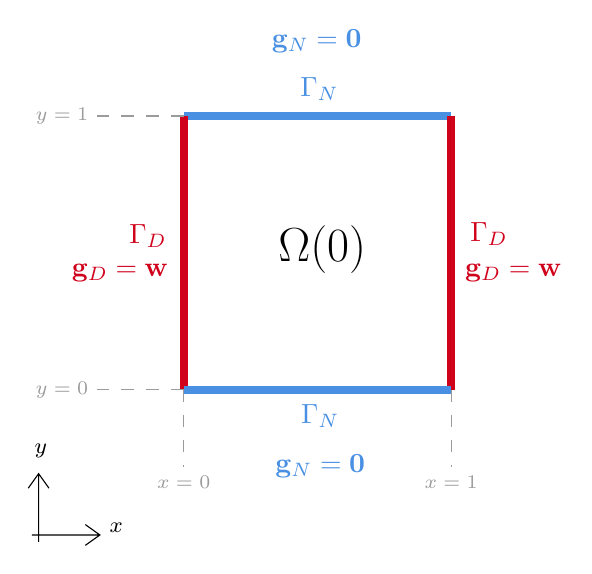
\begin{tikzpicture}[x=0.75pt,y=0.75pt,yscale=-1,xscale=1]
%uncomment if require: \path (0,336); %set diagram left start at 0, and has height of 336

%Straight Lines [id:da3775330886942099] 
\draw [color={rgb, 255:red, 74; green, 144; blue, 226 }  ,draw opacity=1 ][line width=3]    (113.28,81.05) -- (242.14,81.05) ;
%Straight Lines [id:da7311947956092497] 
\draw [color={rgb, 255:red, 208; green, 2; blue, 27 }  ,draw opacity=1 ][line width=3]    (242.14,81.05) -- (242.14,212.95) ;
%Straight Lines [id:da6649609020271117] 
\draw [color={rgb, 255:red, 208; green, 2; blue, 27 }  ,draw opacity=1 ][line width=3]    (113.28,81.05) -- (113.28,212.95) ;
%Straight Lines [id:da0032656115651366058] 
\draw [color={rgb, 255:red, 74; green, 144; blue, 226 }  ,draw opacity=1 ][line width=3]    (242.14,212.95) -- (113.28,212.95) ;
%Shape: Axis 2D [id:dp28368375799841394] 
\draw  (40.08,282.88) -- (72.88,282.88)(43.36,253.36) -- (43.36,286.16) (65.88,277.88) -- (72.88,282.88) -- (65.88,287.88) (38.36,260.36) -- (43.36,253.36) -- (48.36,260.36)  ;

%Straight Lines [id:da4221223762377593] 
\draw [color={rgb, 255:red, 155; green, 155; blue, 155 }  ,draw opacity=1 ] [dash pattern={on 4.5pt off 4.5pt}]  (113.28,212.95) -- (113.28,250) ;
%Straight Lines [id:da5345451203989031] 
\draw [color={rgb, 255:red, 155; green, 155; blue, 155 }  ,draw opacity=1 ] [dash pattern={on 4.5pt off 4.5pt}]  (242.14,212.95) -- (242.14,250) ;
%Straight Lines [id:da5891570191879292] 
\draw [color={rgb, 255:red, 155; green, 155; blue, 155 }  ,draw opacity=1 ] [dash pattern={on 4.5pt off 4.5pt}]  (113.28,212.95) -- (70.5,212.95) ;
%Straight Lines [id:da22019042876536155] 
\draw [color={rgb, 255:red, 155; green, 155; blue, 155 }  ,draw opacity=1 ] [dash pattern={on 4.5pt off 4.5pt}]  (113.28,81.05) -- (70.5,81.05) ;

% Text Node
\draw (106.32,138.93) node [anchor=east] [inner sep=0.75pt]  [color={rgb, 255:red, 208; green, 2; blue, 27 }  ,opacity=1 ]  {$\Gamma _{D}$};
% Text Node
\draw (250.14,138.04) node [anchor=west] [inner sep=0.75pt]  [color={rgb, 255:red, 208; green, 2; blue, 27 }  ,opacity=1 ]  {$\Gamma _{D}$};
% Text Node
\draw (178.66,74.95) node [anchor=south] [inner sep=0.75pt]  [color={rgb, 255:red, 74; green, 144; blue, 226 }  ,opacity=1 ]  {$\Gamma _{N}$};
% Text Node
\draw (179.09,218.96) node [anchor=north] [inner sep=0.75pt]  [color={rgb, 255:red, 74; green, 144; blue, 226 }  ,opacity=1 ]  {$\Gamma _{N}$};
% Text Node
\draw (107.05,150.96) node [anchor=north east] [inner sep=0.75pt]  [color={rgb, 255:red, 208; green, 2; blue, 27 }  ,opacity=1 ]  {$\mathbf{g}_{D} =\mathbf{w}$};
% Text Node
\draw (247.65,150.96) node [anchor=north west][inner sep=0.75pt]  [color={rgb, 255:red, 208; green, 2; blue, 27 }  ,opacity=1 ]  {$\mathbf{g}_{D} =\mathbf{w}$};
% Text Node
\draw (179.08,242.86) node [anchor=north] [inner sep=0.75pt]  [color={rgb, 255:red, 74; green, 144; blue, 226 }  ,opacity=1 ]  {$\mathbf{g}_{N} =\mathbf{0}$};
% Text Node
\draw (177.35,51.93) node [anchor=south] [inner sep=0.75pt]  [color={rgb, 255:red, 74; green, 144; blue, 226 }  ,opacity=1 ]  {$\mathbf{g}_{N} =\mathbf{0}$};
% Text Node
\draw (179.99,145.37) node  [font=\LARGE]  {$\Omega ( 0)$};
% Text Node
\draw (76.26,279.4) node [anchor=west] [inner sep=0.75pt]  [font=\footnotesize]  {$x$};
% Text Node
\draw (44.4,246.95) node [anchor=south] [inner sep=0.75pt]  [font=\footnotesize]  {$y$};
% Text Node
\draw (113.28,253.4) node [anchor=north] [inner sep=0.75pt]  [font=\scriptsize,color={rgb, 255:red, 155; green, 155; blue, 155 }  ,opacity=1 ]  {$x=0$};
% Text Node
\draw (242.14,253.4) node [anchor=north] [inner sep=0.75pt]  [font=\scriptsize,color={rgb, 255:red, 155; green, 155; blue, 155 }  ,opacity=1 ]  {$x=1$};
% Text Node
\draw (68.5,212.95) node [anchor=east] [inner sep=0.75pt]  [font=\scriptsize,color={rgb, 255:red, 155; green, 155; blue, 155 }  ,opacity=1 ]  {$y=0$};
% Text Node
\draw (68.5,81.05) node [anchor=east] [inner sep=0.75pt]  [font=\scriptsize,color={rgb, 255:red, 155; green, 155; blue, 155 }  ,opacity=1 ]  {$y=1$};


\end{tikzpicture}
}
                    \caption{}
                    \label{fig:square-solid-wall:0}
                \end{subfigure}
                \hfill
                \begin{subfigure}{0.53\textwidth}
                    \centering
                    

\tikzset{every picture/.style={line width=0.75pt}} %set default line width to 0.75pt        
\resizebox{\textwidth}{!}{%
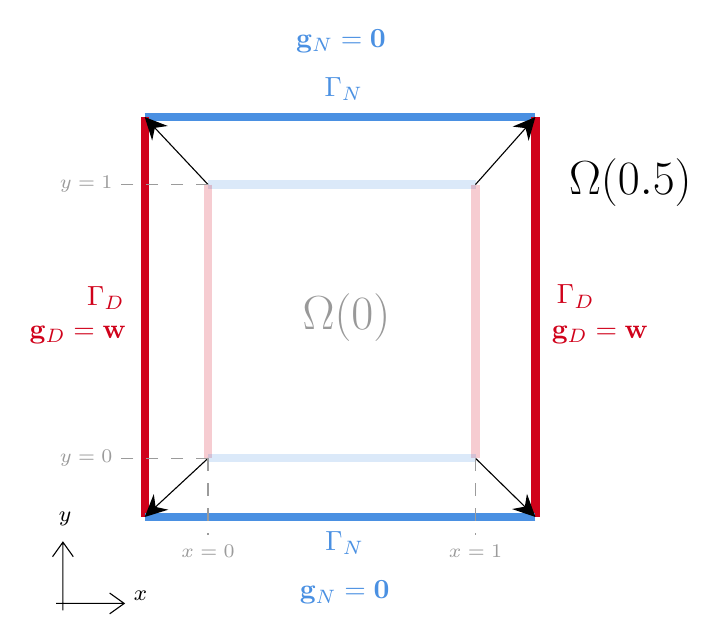
\begin{tikzpicture}[x=0.75pt,y=0.75pt,yscale=-1,xscale=1]
%uncomment if require: \path (0,350); %set diagram left start at 0, and has height of 350

%Straight Lines [id:da3911785235524641] 
\draw [color={rgb, 255:red, 74; green, 144; blue, 226 }  ,draw opacity=1 ][line width=3]    (98.78,72.15) -- (287,72.15) ;
%Straight Lines [id:da08153744945246588] 
\draw [color={rgb, 255:red, 208; green, 2; blue, 27 }  ,draw opacity=1 ][line width=3]    (287,72.15) -- (287,264.82) ;
%Straight Lines [id:da5688674307213424] 
\draw [color={rgb, 255:red, 208; green, 2; blue, 27 }  ,draw opacity=1 ][line width=3]    (98.78,72.15) -- (98.78,264.82) ;
%Straight Lines [id:da13408740199002578] 
\draw [color={rgb, 255:red, 74; green, 144; blue, 226 }  ,draw opacity=1 ][line width=3]    (287,264.82) -- (98.78,264.82) ;
%Straight Lines [id:da8870048899559595] 
\draw [color={rgb, 255:red, 74; green, 144; blue, 226 }  ,draw opacity=0.2 ][line width=3]    (129.28,104.65) -- (258.14,104.65) ;
%Straight Lines [id:da8723650118672401] 
\draw [color={rgb, 255:red, 208; green, 2; blue, 27 }  ,draw opacity=0.2 ][line width=3]    (258.14,104.65) -- (258.14,236.55) ;
%Straight Lines [id:da4357741269330557] 
\draw [color={rgb, 255:red, 208; green, 2; blue, 27 }  ,draw opacity=0.2 ][line width=3]    (129.28,104.65) -- (129.28,236.55) ;
%Straight Lines [id:da9191492030234965] 
\draw [color={rgb, 255:red, 74; green, 144; blue, 226 }  ,draw opacity=0.2 ][line width=3]    (258.14,236.55) -- (129.28,236.55) ;
%Shape: Axis 2D [id:dp9350720821526224] 
\draw  (56.08,306.48) -- (88.88,306.48)(59.36,276.96) -- (59.36,309.76) (81.88,301.48) -- (88.88,306.48) -- (81.88,311.48) (54.36,283.96) -- (59.36,276.96) -- (64.36,283.96)  ;

%Straight Lines [id:da021521710554898155] 
\draw    (129.28,104.65) -- (100.83,74.34) ;
\draw [shift={(98.78,72.15)}, rotate = 46.82] [fill={rgb, 255:red, 0; green, 0; blue, 0 }  ][line width=0.08]  [draw opacity=0] (10.72,-5.15) -- (0,0) -- (10.72,5.15) -- (7.12,0) -- cycle    ;
%Straight Lines [id:da8341315604563517] 
\draw    (258.14,104.65) -- (285.01,74.39) ;
\draw [shift={(287,72.15)}, rotate = 131.61] [fill={rgb, 255:red, 0; green, 0; blue, 0 }  ][line width=0.08]  [draw opacity=0] (10.72,-5.15) -- (0,0) -- (10.72,5.15) -- (7.12,0) -- cycle    ;
%Straight Lines [id:da6015135889734096] 
\draw    (258.14,236.55) -- (284.86,262.72) ;
\draw [shift={(287,264.82)}, rotate = 224.4] [fill={rgb, 255:red, 0; green, 0; blue, 0 }  ][line width=0.08]  [draw opacity=0] (10.72,-5.15) -- (0,0) -- (10.72,5.15) -- (7.12,0) -- cycle    ;
%Straight Lines [id:da44271674446744247] 
\draw    (129.28,236.55) -- (100.98,262.78) ;
\draw [shift={(98.78,264.82)}, rotate = 317.18] [fill={rgb, 255:red, 0; green, 0; blue, 0 }  ][line width=0.08]  [draw opacity=0] (10.72,-5.15) -- (0,0) -- (10.72,5.15) -- (7.12,0) -- cycle    ;
%Straight Lines [id:da8787304201926478] 
\draw [color={rgb, 255:red, 155; green, 155; blue, 155 }  ,draw opacity=1 ] [dash pattern={on 4.5pt off 4.5pt}]  (129.28,236.55) -- (129.28,273.6) ;
%Straight Lines [id:da19489772630369218] 
\draw [color={rgb, 255:red, 155; green, 155; blue, 155 }  ,draw opacity=1 ] [dash pattern={on 4.5pt off 4.5pt}]  (258.14,236.55) -- (258.14,273.6) ;
%Straight Lines [id:da9299742276817373] 
\draw [color={rgb, 255:red, 155; green, 155; blue, 155 }  ,draw opacity=1 ] [dash pattern={on 4.5pt off 4.5pt}]  (129.28,236.55) -- (86.5,236.55) ;
%Straight Lines [id:da941430709775763] 
\draw [color={rgb, 255:red, 155; green, 155; blue, 155 }  ,draw opacity=1 ] [dash pattern={on 4.5pt off 4.5pt}]  (129.28,104.65) -- (86.5,104.65) ;

% Text Node
\draw (90.32,159.53) node [anchor=east] [inner sep=0.75pt]  [color={rgb, 255:red, 208; green, 2; blue, 27 }  ,opacity=1 ]  {$\Gamma _{D}$};
% Text Node
\draw (296.14,158.64) node [anchor=west] [inner sep=0.75pt]  [color={rgb, 255:red, 208; green, 2; blue, 27 }  ,opacity=1 ]  {$\Gamma _{D}$};
% Text Node
\draw (194.66,65.55) node [anchor=south] [inner sep=0.75pt]  [color={rgb, 255:red, 74; green, 144; blue, 226 }  ,opacity=1 ]  {$\Gamma _{N}$};
% Text Node
\draw (195.09,270.56) node [anchor=north] [inner sep=0.75pt]  [color={rgb, 255:red, 74; green, 144; blue, 226 }  ,opacity=1 ]  {$\Gamma _{N}$};
% Text Node
\draw (91.05,171.56) node [anchor=north east] [inner sep=0.75pt]  [color={rgb, 255:red, 208; green, 2; blue, 27 }  ,opacity=1 ]  {$\mathbf{g}_{D} =\mathbf{w}$};
% Text Node
\draw (293.65,171.56) node [anchor=north west][inner sep=0.75pt]  [color={rgb, 255:red, 208; green, 2; blue, 27 }  ,opacity=1 ]  {$\mathbf{g}_{D} =\mathbf{w}$};
% Text Node
\draw (195.08,294.46) node [anchor=north] [inner sep=0.75pt]  [color={rgb, 255:red, 74; green, 144; blue, 226 }  ,opacity=1 ]  {$\mathbf{g}_{N} =\mathbf{0}$};
% Text Node
\draw (193.35,42.53) node [anchor=south] [inner sep=0.75pt]  [color={rgb, 255:red, 74; green, 144; blue, 226 }  ,opacity=1 ]  {$\mathbf{g}_{N} =\mathbf{0}$};
% Text Node
\draw (195.99,168.97) node  [font=\LARGE,color={rgb, 255:red, 0; green, 0; blue, 0 }  ,opacity=0.4 ]  {$\Omega ( 0)$};
% Text Node
\draw (301.93,103.47) node [anchor=west] [inner sep=0.75pt]  [font=\LARGE,color={rgb, 255:red, 0; green, 0; blue, 0 }  ,opacity=1 ]  {$\Omega ( 0.5)$};
% Text Node
\draw (129.28,277) node [anchor=north] [inner sep=0.75pt]  [font=\scriptsize,color={rgb, 255:red, 155; green, 155; blue, 155 }  ,opacity=1 ]  {$x=0$};
% Text Node
\draw (258.14,277) node [anchor=north] [inner sep=0.75pt]  [font=\scriptsize,color={rgb, 255:red, 155; green, 155; blue, 155 }  ,opacity=1 ]  {$x=1$};
% Text Node
\draw (84.5,236.55) node [anchor=east] [inner sep=0.75pt]  [font=\scriptsize,color={rgb, 255:red, 155; green, 155; blue, 155 }  ,opacity=1 ]  {$y=0$};
% Text Node
\draw (84.5,104.65) node [anchor=east] [inner sep=0.75pt]  [font=\scriptsize,color={rgb, 255:red, 155; green, 155; blue, 155 }  ,opacity=1 ]  {$y=1$};
% Text Node
\draw (92.26,303) node [anchor=west] [inner sep=0.75pt]  [font=\footnotesize]  {$x$};
% Text Node
\draw (60.4,270.55) node [anchor=south] [inner sep=0.75pt]  [font=\footnotesize]  {$y$};


\end{tikzpicture}
}
                    \caption{}
                    \label{fig:square-solid-wall:later}
                \end{subfigure}
                \caption{Visualisation of the boundary conditions applied to the problem described in \S\ref{sec:contractions:numerical-experiments:boundary-movement}, which applies a zero Neumann condition on the top and bottom sides of the domain, and a no-slip Dirichlet condition on the left and right sides. $\Omega$ is shown at times (a) $t=0$, and (b) $t=0.5$ for the domain velocity detailed in Equation \eqref{eq:oscillating-mesh-velocity} and \S\ref{sec:contractions:numerical-experiments:boundary-movement}.}
                \label{fig:square-solid-wall}
            \end{figure}
            
            We begin the simulation with an initial condition of $\vec{u}_h^0 \equiv \vec{0}$ and run between times $t \in [0, 1]$, with time-step size $\Delta t = 0.01$. We select the domain velocity $\vec{w} \equiv (w_1, w_2)^\intercal$ as
            \begin{subequations}
                \begin{equation}
                    w_1 = W (x - x_c) \sin\left(\frac{2 \pi t - T_0}{T}\right),
                    \label{eq:oscillating-mesh-velocity:1}
                \end{equation}
                \begin{equation}
                    w_2 = W (y - y_c) \sin\left(\frac{2 \pi t - T_0}{T}\right),
                    \label{eq:oscillating-mesh-velocity:2}
                \end{equation}%
                \label{eq:oscillating-mesh-velocity}%
            \end{subequations}%
            where we select $x_c = y_c = 0.5$, $T_0 = 0$, $T = 1$, and $W = 1$ here. This domain velocity corresponds to smooth expansion and contraction about centre $(x_c, y_c) = (0.5, 0.5)$ for $t \in [0, 1]$, with a minimal domain area of $\Omega$ at $t = 0$ and $t=1$, and a maximal area at $t = 0.5$. Furthermore, we note that this gives a maximal rate of expansion at $t = 0.25$ and maximal rate of deflation at $t = 0.75$. The maximum domain size at $t=0.5$ is visualised in Figure \ref{fig:square-solid-wall:later}.
            
            Figures \ref{fig:square-solid-wall-flow:02}--\ref{fig:square-solid-wall-flow:75} respectively visualise the flow at times $t=0.02$, $t=0.25$, $t=0.52$, and $t=0.75$. A video visualising the velocity field through time at every time-step is available here\footnote{\url{https://r.blakey.family/phd-video-mmv-square}}. At $t = 0.02$, Figure \ref{fig:square-solid-wall-flow:02} shows the flow drawn through the top and bottom sides and aligning in the direction of the domain velocity on the boundary, which is at that moment pointing outward from the centre of the square domain. The domain velocity then accelerates up to a maximum domain velocity at $t = 0.25$, as illustrated in Figure \ref{fig:square-solid-wall-flow:25}, which shows high-speed blood concentrated in the centre of the top and bottom sides, and also in the four corners of the domain. The domain velocity then decelerates as the area reaches its maximum size at $t=0.5$; Figure \ref{fig:square-solid-wall-flow:52} shows the velocity field at $t = 0.52$, just after the maximum area is reached, where we note the reversal in the streamline directions as the domain begins to contract and eject flow out of the top and bottom sides. Finally, Figure \ref{fig:square-solid-wall-flow:75} shows the domain at $t = 0.75$ at the most rapid point of contraction, which unsurprisingly looks very similar to the flow at $t=0.25$ except for a reversal in flow direction.
            
            \begin{figure}
                \begin{centering}
                    %%%%%
                    \begin{subfigure}{0.45\textwidth}
                        \begin{centering}
                            \includegraphics[width=\textwidth]{diagrams/results-contractions/mm_5_white.0002.png}
                            \caption{}
                            \label{fig:square-solid-wall-flow:02}
                        \end{centering}
                    \end{subfigure}
                    \begin{subfigure}{0.45\textwidth}
                        \begin{centering}
                            \includegraphics[width=\textwidth]{diagrams/results-contractions/mm_5_black.0025.png}
                            \caption{}
                            \label{fig:square-solid-wall-flow:25}
                        \end{centering}
                    \end{subfigure}
                    \begin{subfigure}{0.45\textwidth}
                        \begin{centering}
                            \includegraphics[width=\textwidth]{diagrams/results-contractions/mm_5_white.0052.png}
                            \caption{}
                            \label{fig:square-solid-wall-flow:52}
                        \end{centering}
                    \end{subfigure}
                    \begin{subfigure}{0.45\textwidth}
                        \begin{centering}
                            \includegraphics[width=\textwidth]{diagrams/results-contractions/mm_5_black.0075.png}
                            \caption{}
                            \label{fig:square-solid-wall-flow:75}
                        \end{centering}
                    \end{subfigure}
                \end{centering}
                \caption{Visualisations of flow for four instances in time for the problem in \S\ref{sec:contractions:numerical-experiments:boundary-movement}. (a)-(d) respectively show flow at $t=0.02$, $t=0.25$, $t=0.52$, $t=0.75$. Linear colour scaling is shown for $|\vec{u}| \in [0, 1]$ with black or white streamlines shown on top. Axes are shown surrounding the domain, showing the domain of size $\Omega = [0, 1]^2$ at $t \approx 0$ and $\Omega \approx [-0.2, 1.2]^2$ at $t \approx 0.5$.}
                \label{fig:square-solid-wall-flow}
            \end{figure}

            In order to model flow in a contracting placenta, we will now apply the numerical methods from \S\ref{sec:contractions:dgfem-discretisation} to NSD with placental flow parameters and the asymmetric placenta problem from \S\ref{sec:numerical-methods:blood-flow-experiments:asymmetric}.

    \section{Preliminary utero-placental pump motion} \label{sec:contractions:placenta}
        The utero-placental pump (or placental contraction) is a newly discovered phenomenon, first reported by \citeauthor{dellschaftHaemodynamicsHumanPlacenta2020} \cite{dellschaftHaemodynamicsHumanPlacenta2020} in \citeyear{dellschaftHaemodynamicsHumanPlacenta2020}. This phenomenon is distinct from other types of contractions, as it involves contractions of the placenta, rather than contractions such as Braxton-Hicks contractions, which instead involve contractions of the entire uterus \cite{togashiSustainedUterineContractions1993}. \citeauthor{dellschaftHaemodynamicsHumanPlacenta2020} \cite{dellschaftHaemodynamicsHumanPlacenta2020} reported that the placenta was observed over $10$-minute intervals to periodically reduce by up to $40\%$ in volume, resulting in the periodic ejection of blood from the IVS. The mechanism of these contractions is not yet known, but it is thought that these contractions may be related to previous reports of contracting villous trees \cite{farleyContractilePropertiesHuman2004,dellschaftHaemodynamicsHumanPlacenta2020}. One theory of the evolutionary role of these contractions is that they assist maternal circulation by ejecting stagnant deoxygenated blood so that it may be replaced by freshly oxygenated blood; however, this is yet to be shown experimentally \cite{dellschaftHaemodynamicsHumanPlacenta2020}.

        In this section, we will prescribe a simple domain velocity that is inspired by MRI scan data. Using this domain velocity, we will then compute the resulting flow and oxygen concentration fields using the moving mesh discretisation presented in \S\ref{sec:contractions:dgfem-discretisation}.

        \subsection{Selection of domain velocity} \label{sec:contractions:placenta:mesh-velocity}
            We begin by using the data from \citeauthor{gowlandCharacterisingPlacentalContractions2024} \cite{gowlandCharacterisingPlacentalContractions2024}, which is reproduced in Figure \ref{fig:contraction-data:raw} and shows various quantities calculated from MRI scan data during a placental contraction. We choose to focus specifically on the volume change during the period of fastest volume reduction, which is indicated in the black box. The volume change data here is calculated by tracing the placenta outline of a 3D stack of 2D MRI scan images, and is measured against the initial placental volume calculated at time $t = 0$.

            \begin{figure}
                \centering
                \begin{subfigure}{\textwidth}
                    \centering
                    

\tikzset{every picture/.style={line width=0.75pt}} %set default line width to 0.75pt        

\begin{tikzpicture}[x=0.75pt,y=0.75pt,yscale=-1,xscale=1]
%uncomment if require: \path (0,300); %set diagram left start at 0, and has height of 300

%Image [id:dp23581150653458827] 
\draw (294.71,143) node  {\includegraphics[width=415.07pt,height=198pt]{diagrams/other-paper-figures/gowland2024_contraction-data.png}};
%Shape: Rectangle [id:dp0616002982809305] 
\draw  [line width=3]  (285,107) -- (347,107) -- (347,230) -- (285,230) -- cycle ;
%Shape: Rectangle [id:dp37370129948188047] 
\draw  [draw opacity=0][fill={rgb, 255:red, 0; green, 0; blue, 0 }  ,fill opacity=0.2 ] (18,11) -- (108.67,11) -- (108.67,274) -- (18,274) -- cycle ;
%Shape: Rectangle [id:dp08993919230122849] 
\draw  [draw opacity=0][fill={rgb, 255:red, 0; green, 0; blue, 0 }  ,fill opacity=0.2 ] (347,11) -- (571,11) -- (571,274) -- (347,274) -- cycle ;
%Shape: Rectangle [id:dp06260699697048411] 
\draw  [draw opacity=0][fill={rgb, 255:red, 0; green, 0; blue, 0 }  ,fill opacity=0.2 ] (285.33,11) -- (347,11) -- (347,107) -- (285.33,107) -- cycle ;
%Shape: Rectangle [id:dp8344768536283782] 
\draw  [draw opacity=0][fill={rgb, 255:red, 0; green, 0; blue, 0 }  ,fill opacity=0.2 ] (285.33,230.33) -- (347,230.33) -- (347,274) -- (285.33,274) -- cycle ;
%Shape: Rectangle [id:dp7625893108020545] 
\draw  [line width=3]  (108.33,182.67) -- (208.67,182.67) -- (208.67,197.67) -- (108.33,197.67) -- cycle ;
%Shape: Rectangle [id:dp9788521517108135] 
\draw  [draw opacity=0][fill={rgb, 255:red, 0; green, 0; blue, 0 }  ,fill opacity=0.2 ] (208.67,11) -- (285.33,11) -- (285.33,274) -- (208.67,274) -- cycle ;
%Shape: Rectangle [id:dp9892312056868955] 
\draw  [draw opacity=0][fill={rgb, 255:red, 0; green, 0; blue, 0 }  ,fill opacity=0.2 ] (108.67,11) -- (208.67,11) -- (208.67,181) -- (108.67,181) -- cycle ;
%Shape: Rectangle [id:dp472204421176478] 
\draw  [draw opacity=0][fill={rgb, 255:red, 0; green, 0; blue, 0 }  ,fill opacity=0.2 ] (108.67,197.67) -- (208.67,197.67) -- (208.67,274) -- (108.67,274) -- cycle ;




\end{tikzpicture}

                    \caption{}
                    \label{fig:contraction-data:raw}
                \end{subfigure}
                \begin{subfigure}{\textwidth}
                    \centering
                    \includegraphics[width=0.75\textwidth]{diagrams/results-contractions/extracted-contraction-data.png}
                    \caption{}
                    \label{fig:contraction-data:extracted}
                \end{subfigure}
                \caption{(a) Graph taken from \citeauthor{gowlandCharacterisingPlacentalContractions2024} \cite{gowlandCharacterisingPlacentalContractions2024} and overlaid with a black box to indicate the region we are interested in modelling in this thesis. Specifically, this is the placental volume change during the period of fastest volume reduction of a placental contraction between approximately $15$ and $16$ minutes. (b) A simpler visualisation of (a) on the region of interest. \S\ref{sec:contractions:placenta:mesh-velocity} describes the simplifications we make of assuming a linear decrease in volume during the period of fastest volume decrease (indicated by the red dotted line), and an appropriate area decrease for an equivalent 2D area change for this 3D volume change (indicated by the green cross). We then assume that the areas and volumes increase at the same rate, back to their original sizes at $t = 17.9$ minutes. Grey vertical lines indicate the snapshots at which Figures \ref{fig:moving-mesh-placenta-velocity} and \ref{fig:moving-mesh-placenta-transport} are visualised.}
                \label{fig:contraction-data}
            \end{figure}
            
            For ease of presentation, we plot again the volume change data points in this region of interest in Figure \ref{fig:contraction-data:extracted}, plotted using blue lines. This shows the largest volume change of $-33.8\%$ at $t=16.1$ minutes. Prior to this, there is a roughly linear decrease in volume from $t=14.8$ minutes. Extrapolating the straight line passing through both of these points (red dotted line), we find the point at which this line meets the horizontal axis to be at $t = 14.3$ minutes (red dot). We make the assumption that the volume increase after a placental contraction is at the same rate as the volume decrease. We therefore model the contraction behaviour between $T_0:=14.3$ and $T_N:=17.9$ minutes, with maximum volume at times $T_0$ and $T_N$ minutes, and a minimum volume at $\frac{T_0+T_N}{2}=16.1$ minutes.

            A complication with using this data is that it concerns a 3D volume. We therefore need to calculate an analogous 2D area change to an equivalent 3D volume. Denoting percentage change in a 2D area by $\Delta_2$, and percentage change in 3D volume by $\Delta_3$, we assume for simplicity that the relationship between a 2D area change and 3D volume change is given through the following relationship:
            \begin{equation}
                (1 + \Delta_2)^{\frac{1}{2}} = (1 + \Delta_3)^{\frac{1}{3}}.
                \label{eq:2D-area-change-to-3D-volume-change}
            \end{equation}
            In our case, $\Delta_3 = -33.8\%$ at the smallest measured volume, which through Equation \eqref{eq:2D-area-change-to-3D-volume-change} gives a 2D area change of $\Delta_2 = -24.0\%$, which is indicated in Figure \ref{fig:contraction-data:extracted} with a green cross.

            Next, we prescribe a domain velocity. For simplicity, we assume that the placenta contracts uniformly in both directions and follows a sinusoidal speed through time. We therefore select the domain velocity $\vec{w} \equiv (w_1, w_2)^\intercal$ from \S\ref{sec:contractions:numerical-experiments:boundary-movement}:
            \begin{subequations}
                \begin{equation}
                    \retag{eq:oscillating-mesh-velocity:1}
                    w_1 = W (x - x_c) \sin\left(\frac{2 \pi t - T_0}{T}\right),
                \end{equation}
                \begin{equation}
                    \retag{eq:oscillating-mesh-velocity:2}
                    w_2 = W (y - y_c) \sin\left(\frac{2 \pi t - T_0}{T}\right),
                \end{equation}
            \end{subequations}
            where $(x_c, y_c)$ is selected as a centre of inflation within the 2D placenta, $T_0=14.3$ and $T = T_N - T_0 = 3.6$ minutes, and $W$ is chosen appropriately such that at time $\frac{T_0+T_N}{2}$ minutes there is a 2D area change of $\Delta_2 = -24.0\%$; here, this corresponds to $W = \qty{8.04e-5}{\metre\per\second}$.
            
            To summarise, we have used MRI scan data of placental volume change during a placental contraction to inform a domain velocity for use in our mathematical model. Specifically, we made a simplification to only consider the period of fastest volume decrease in this data, and calculated an equivalent area change for our 2D geometry from this 3D data. We then selected a simple form of domain velocity that gives an equivalent maximum area reduction on our 2D placenta geometry between $T_0 = 14.3$ and $T_N = 17.9$ minutes.

            We will now introduce the problem we aim to address.

        \subsection{Problem setup} \label{sec:contractions:placenta:problem-setup}
            Using the domain velocity from \S\ref{sec:contractions:placenta:mesh-velocity}, we will now specify the moving boundary problem we intend to compute approximations to.
            
            For the flow problem, we consider a small modification to the boundary conditions to those presented in \S\ref{sec:modelling:blood-flow:boundary-conditions}. We recall boundary conditions are applied in the form
            \begin{subequations}
                \begin{alignat*}{3}
                    \left( \nabla \vec{u} - p \mat{I} \right) \cdot \vec{n} & = \vec{g}_\text{f,N} &&~ \text{on } \Gamma_\text{out}, \\
                    \vec{u} & = \vec{g}_\text{f,D} &&~ \text{on } \Gamma\setminus\Gamma_\text{out},
                \end{alignat*}%
            \end{subequations}%
            and we select these boundary condition functions such that there is a zero Neumann condition on outflow, a parabolic inflow velocity profile, and no velocity slip elsewhere. We additionally choose the amplitude of this parabolic inflow such that the flux of incoming blood is constant through time. We note that, in order to impose no-slip boundary conditions on solid walls, the velocity must take the value of the domain velocity $\vec{w}$ at the boundary. The modified boundary conditions for this moving boundary problem are given by
            \begin{subequations}
                \begin{alignat}{3}
                    \vec{g}_\text{f,D} & = - A(t) \frac{R(t)^2 - r^2}{R(t)^2} \vec{n} &&~ \text{on } \Gamma_\text{in}, \\
                    \vec{g}_\text{f,N} & = \vec{0} &&~ \text{on } \Gamma_\text{out},\\
                    \vec{g}_\text{f,D} & = \vec{w} &&~ \text{on } \Gamma \setminus (\Gamma_\text{in} \cup \Gamma_\text{out}),
                \end{alignat}%
            \end{subequations}%
            where $\vec{n}$ is the unit outward-pointing normal on $\Gamma_\text{in}$, $r(\vec{x})$ is the distance from a point $\vec{x}$ to the centre of $\Gamma_\text{in}$, $R(t)$ is the artery radius, and $A(t) := \frac{R(0)}{R(t)}$ is the modified amplitude of the Poiseuille flow to retain constant inlet flux.

            For the oxygen transport problem, we keep the same boundary conditions as those presented in \S\ref{sec:modelling:transport}; namely, boundary conditions are applied of the form
            \begin{subequations}
                \begin{alignat*}{3}
                    c & = g_\text{c,D} &&~ \text{on } \Gamma_\text{in}, \\
                    \nabla c \cdot \vec{n} & = g_\text{c,N} &&~ \text{on } \Gamma\setminus\Gamma_\text{in},
                \end{alignat*}%
            \end{subequations}
            and the boundary condition functions are given as
            \begin{subequations}
                \begin{alignat}{3}
                    g_\text{c,D} & = 1 &&~ \text{on } \Gamma_\text{in},\retag{eq:oxygen-bcs:dirichlet}\\
                    g_\text{c,N} & = 0 &&~ \text{on } \Gamma\setminus\Gamma_\text{in}.\retag{eq:oxygen-bcs:neumann}%
                \end{alignat}%
            \end{subequations}%

            We will now use the prescribed domain velocity from \S\ref{sec:contractions:placenta:mesh-velocity} and the problem setup presented here, together with the numerical methods from \S\ref{sec:contractions:dgfem-discretisation}, to compute the blood flow and oxygen transport fields under this domain movement.

        \subsection{Placenta motion}
            We take our initial domain $\Omega^0$ to be the 2D placenta domain with dimensions specified in \S\ref{sec:modelling:geometries:2d-placenta} and asymmetric placement of vessels as presented in \S\ref{sec:numerical-methods:blood-flow-experiments:asymmetric}. We use the steady-state approximations on $\Omega^0$ as the initial conditions for the time-dependent blood flow and oxygen concentration problems. For these simulations, we have selected a time-step size of $\Delta t = \qty{0.036}{\minute} = \qty{2.16}{\second}$. We note that each time-step is longer than a typical cardiac cycle, and we therefore do not apply any corresponding adjustment to the amplitude to account for pulsatile inlet flow. We chose this relatively large time-step size for simplicity, and because of the relatively slow domain velocity scaling of $W = \qty{8.04e-5}{\metre\per\second}$.

            We will consider only five snapshots in time in the body of this thesis for ease of presentation. Videos visualising these fields through time at every time-step are available here\footnote{Blood flow field: \url{https://r.blakey.family/phd-video-mmv}; oxygen transport field: \url{https://r.blakey.family/phd-video-mmt}}. Figures \ref{fig:moving-mesh-placenta-velocity} and \ref{fig:moving-mesh-placenta-transport} provide the main results of this chapter. These figures respectively visualise the blood flow and oxygen transport fields in five snapshots in time, which are indicated in Figure \ref{fig:contraction-data:extracted} by grey vertical lines.

            \begin{figure}
                \centering
                \begin{subfigure}{\textwidth}
                    \includegraphics[width=\textwidth]{diagrams/results-contractions/placenta-moving-mesh/mm-placenta-velocity.0000.png}
                    \caption{}
                    \label{fig:moving-mesh-placenta-velocity:1}
                \end{subfigure}
                \begin{subfigure}{\textwidth}
                    \includegraphics[width=\textwidth]{diagrams/results-contractions/placenta-moving-mesh/mm-placenta-velocity.0025.png}
                    \caption{}
                    \label{fig:moving-mesh-placenta-velocity:2}
                \end{subfigure}
                \begin{subfigure}{\textwidth}
                    \includegraphics[width=\textwidth]{diagrams/results-contractions/placenta-moving-mesh/mm-placenta-velocity.0050.png}
                    \caption{}
                    \label{fig:moving-mesh-placenta-velocity:3}
                \end{subfigure}
                \begin{subfigure}{\textwidth}
                    \includegraphics[width=\textwidth]{diagrams/results-contractions/placenta-moving-mesh/mm-placenta-velocity.0095.png}
                    \caption{}
                    \label{fig:moving-mesh-placenta-velocity:4}
                \end{subfigure}
                \begin{subfigure}{\textwidth}
                    \includegraphics[width=\textwidth]{diagrams/results-contractions/placenta-moving-mesh/mm-placenta-velocity.0100.png}
                    \caption{}
                    \label{fig:moving-mesh-placenta-velocity:5}
                \end{subfigure}
                \caption{Visualisation of the blood flow field during a contraction at times (a) $t=\qty{14.30}{\minute}$, (b) $t=\qty{15.20}{\minute}$, (c) $t=\qty{16.10}{\minute}$, (d) $t=\qty{17.72}{\minute}$, and (e) $t=\qty{17.9}{\minute}$. Colours are logarithmically scaled, and streamlines at each time-step are shown with black lines. A video visualising all time-steps can be viewed here: \url{https://r.blakey.family/phd-video-mmv}}
                \label{fig:moving-mesh-placenta-velocity}
            \end{figure}

            \begin{figure}
                \centering
                \begin{subfigure}{\textwidth}
                    \includegraphics[width=\textwidth]{diagrams/results-contractions/placenta-moving-mesh/mm-placenta-transport.0000.png}
                    \caption{}
                    \label{fig:moving-mesh-placenta-transport:1}
                \end{subfigure}
                \begin{subfigure}{\textwidth}
                    \includegraphics[width=\textwidth]{diagrams/results-contractions/placenta-moving-mesh/mm-placenta-transport.0025.png}
                    \caption{}
                    \label{fig:moving-mesh-placenta-transport:2}
                \end{subfigure}
                \begin{subfigure}{\textwidth}
                    \includegraphics[width=\textwidth]{diagrams/results-contractions/placenta-moving-mesh/mm-placenta-transport.0050.png}
                    \caption{}
                    \label{fig:moving-mesh-placenta-transport:3}
                \end{subfigure}
                \begin{subfigure}{\textwidth}
                    \includegraphics[width=\textwidth]{diagrams/results-contractions/placenta-moving-mesh/mm-placenta-transport.0095.png}
                    \caption{}
                    \label{fig:moving-mesh-placenta-transport:4}
                \end{subfigure}
                \begin{subfigure}{\textwidth}
                    \includegraphics[width=\textwidth]{diagrams/results-contractions/placenta-moving-mesh/mm-placenta-transport.0100.png}
                    \caption{}
                    \label{fig:moving-mesh-placenta-transport:5}
                \end{subfigure}
                \caption{Visualisation of the oxygen concentration field during a contraction at times (a) $t=\qty{14.30}{\minute}$, (b) $t=\qty{15.20}{\minute}$, (c) $t=\qty{16.10}{\minute}$, (d) $t=\qty{17.72}{\minute}$, and (e) $t=\qty{17.9}{\minute}$. Colours are linearly scaled. A video visualising all time-steps can be viewed here: \url{https://r.blakey.family/phd-video-mmt}}
                \label{fig:moving-mesh-placenta-transport}
            \end{figure}

            Panel (a) of Figures \ref{fig:moving-mesh-placenta-velocity} and \ref{fig:moving-mesh-placenta-transport} give the initial steady-state fields of the flow and oxygen concentration, respectively; we remark that these fields are identical to the fields presented in \S\ref{sec:numerical-methods:blood-flow-experiments:asymmetric} and \S\ref{sec:numerical-methods:time-dependent-experiments}.
            
            Despite the varying domain size, the blood flow field changes very little from the steady-state solution as time progresses, with only small changes in the slower regions of the domain; an example of a small change in flow is shown in Figure \ref{fig:moving-mesh-placenta-velocity:2}, where previously slow blood near septal walls is advected by the moving boundary at a slightly higher speed.
            
            On the other hand, the oxygen concentration field changes noticeably more, with clear changes in the solution between each of the five snapshots in time. Figure \ref{fig:moving-mesh-placenta-transport:2} shows the oxygen concentration field at time $t = T_0 + \frac{T}{4}$, which corresponds to the point of fastest domain decrease due to the sinusoidal domain velocity. Here, we see oxygen advected away from the basal plate, leaving small regions on the basal plate where no oxygen is present. It is interesting to see in this snapshot that there is a change near recirculation zones in the central cavities, where high concentrations of oxygen become encircled by lower concentration oxygen. As the oxygen concentration field evolves from Figure \ref{fig:moving-mesh-placenta-transport:1} to Figure \ref{fig:moving-mesh-placenta-transport:3}, the furthest right placentone contains a region to the left of the artery where oxygen concentration reduces over time; this is because oxygen is uptaken by the villous tree here and oxygen is not being replaced. As time progresses and the domain enlarges to Figure \ref{fig:moving-mesh-placenta-transport:5}, this region is again filled with oxygen.

            Overall, the oxygen concentration appears to decrease whilst the domain contracts, and appears to fill more of the domain in higher concentration during the latter domain expansion. To solidify our understanding of this and the effect on flow speed, we measure both the average speed and the uptake by the villous tree at each instant in time. Although each of the two previous chapters are distinct from the work presented here, we restate two of the efficiency measures from Chapter \ref{sec:nutrient-uptake}, which respectively give instantaneous measures of the speed and amount of oxygen uptaken by the entire villous tree:
            \begin{align}
                \bar{v}(\Omega) & := \frac{1}{|\Omega|} \int_{\Omega} |\vec{u}| \diff \vec{x}, \retag{eq:eff-v} \\
                \bar{c} & := \frac{R}{|\Omega|} \int_\Omega \Psi c \diff \vec{x}, \retag{eq:eff-c}
            \end{align}
            where $\vec{u}$ is the velocity of the blood flow, $c$ is the oxygen concentration field, $|\Omega| := \int_\Omega \diff \vec{x}$, $R$ is the uptake rate of the villous tree from Table \ref{tab:problem-parameters}, and $\Psi$ defines the smooth transition region described in \S\ref{sec:modelling:blood-flow}. Figures \ref{fig:mm-quantities:velocity} and \ref{fig:mm-quantities:uptake} respectively visualise $\bar{v}(\Omega)$ and $\bar{c}$ through our simulation.

            \begin{figure}
                %% MONOLITH COMMIT:
                %% File run: ./plotting/mm-quantities.py
                %% Date run: 2024-05-10 12:33:00
                \centering
                \begin{subfigure}{0.45\textwidth}
                    \includegraphics[width=\textwidth]{diagrams/results-contractions/mm-quantities-velocity.png}
                    \caption{}
                    \label{fig:mm-quantities:velocity}
                \end{subfigure}
                \begin{subfigure}{0.45\textwidth}
                    \includegraphics[width=\textwidth]{diagrams/results-contractions/mm-quantities-uptake.png}
                    \caption{}
                    \label{fig:mm-quantities:uptake}
                \end{subfigure}
                \caption{Graphs show how (a) $\bar{v}(\Omega)$ (Equation \eqref{eq:eff-v}) and (b) $\bar{c}$ (Equation \eqref{eq:eff-c}) vary throughout a contraction of the problem presented in \S\ref{sec:contractions:placenta}. Horizontal dotted lines indicate the value of these measures at time $t = T_0$.}
                \label{fig:mm-quantities}
            \end{figure}

            Figure \ref{fig:mm-quantities:velocity} shows that the average speed of the blood increases when the domain contracts, and decreases again when the domain expands. Interestingly, the peak of $\bar{v}(\Omega)$ corresponds to $t = \qty{15.9}{\minute}$, which is $\qty{0.2}{\minute}$ before the domain is at its smallest; as the domain velocity is decelerating toward this minimal domain size, this could be due to inertial effects on the blood which cause an augmented maximum. Likewise, there is a minimum $\qty{0.2}{\minute}$ before the maximum domain size is regained at $t = \qty{17.9}{\minute}$.
            
            Figure \ref{fig:mm-quantities:uptake} shows slightly different behaviour, where oxygen uptake is lowest during the period of most rapid contraction and highest during the period of most rapid expansion; these correspond to what we saw when visualising the oxygen concentration field in Figure \ref{fig:moving-mesh-placenta-transport:5}, where certain areas of the domain appeared to have lower oxygen concentration during the contraction and higher oxygen concentration during the expansion. The most significant feature of this graph is that the oxygen uptake is increased when the placenta returns to its original size at $t = \qty{17.9}{\minute}$, indicated by the solid line being higher than the dotted line. This simulation therefore supports the theory that placental contractions could assist maternal circulation by ejecting stagnant deoxygenated blood and improve oxygen delivery to the fetus \cite{dellschaftHaemodynamicsHumanPlacenta2020}.

            We will now close this chapter with some closing remarks, limitations of our contraction model, and suggested future work.

    \section{Summary} \label{sec:contractions:summary}
        In this chapter, we have introduced a basic model of prescribed boundary motion in order to investigate the effects of the recently-observed `utero-placental pump' contractions on maternal blood flow and oxygen transport dynamics. These are contractions that involve only the placenta and have been observed over $10$-minute intervals to periodically reduce placental volume by up to $40\%$ \cite{dellschaftHaemodynamicsHumanPlacenta2020}.

        In \S\ref{sec:contractions:dgfem-discretisation}, we used the Reynolds Transport Theorem to derive modified numerical methods for the flow and oxygen transport problem, which were valid on moving domains, and required minimal modification to the existing semilinear and bilinear forms of the discretisation. We then validated our numerical methods in \S\ref{sec:contractions:numerical-experiments} in two different ways: first, we used the method of manufactured solution (MMS) and showed that we obtain optimal spatial and temporal convergence rates under refinement; and secondly, we presented a physical problem where no-slip boundary conditions on an oscillating wall influence flow dynamics, which gave physically sensible flow dynamics.

        The main results of the chapter were presented in \S\ref{sec:contractions:placenta}, where we used volume information from MRI scan data to inform a domain velocity that represents a domain size change comparable to those found during a `utero-placental pump' contraction. Our results found that the blood flow field remained largely undisturbed, despite the relatively large domain size change; we noted that this is likely due to the long timescales upon which these contractions take place. We did, however, find that the oxygen concentration field was more visibly influenced by the boundary motion than the velocity field, with overall decreased oxygen uptake during the contracting phase and increased oxygen uptake during the expansion phase. Our simulation showed that contractions of this form do have an impact on oxygen concentration dynamics and oxygen uptake by the villous tree.

        For clarity, the model of the utero-placental pump we have presented here is highly simplified and does not consider the physical mechanisms driving the contractions. In particular, we have assumed a simple form for the domain velocity, and used this over a shorter \qty{3.6}{\minute} period covering the fastest volume change rate, rather than the full \qty{26}{\minute} presented in the data of \citeauthor{gowlandCharacterisingPlacentalContractions2024} \cite{gowlandCharacterisingPlacentalContractions2024}. Furthermore, the results of \citeauthor{dellschaftHaemodynamicsHumanPlacenta2020} \cite{dellschaftHaemodynamicsHumanPlacenta2020} show very little change in the thickness of the placenta between the chorionic and basal plates, with the contraction primarily taking place in the horizontal direction (when viewed in the orientation we have presented in this thesis); future work taking this approach could therefore simulate the entire contraction length and consider domain velocities that cause shape change only in the horizontal direction. Additionally, future studies could investigate the effect that villous tree density and shape has on flow dynamics and oxygen uptake.

        The cause of these contractions is currently unknown \cite{dellschaftHaemodynamicsHumanPlacenta2020}, but it is thought that they may be related to previous reports of contracted villous trees, which are sometimes anchored (i.e., connected) to the basal plate \cite{dellschaftHaemodynamicsHumanPlacenta2020,katoVillousTreeModel2017}. An interesting extension to this work would be to use the work of \citeauthor{katoVillousTreeModel2017} \cite{katoVillousTreeModel2017} in designing a model of the utero-placental pump that respects the data of \citeauthor{gowlandCharacterisingPlacentalContractions2024} \cite{gowlandCharacterisingPlacentalContractions2024}. An alternative modelling approach could reapply one of the works from the existing fluid-structure interaction literature (e.g., \cite{houNumericalMethodsFluidStructure2012,doneaArbitraryLagrangianEulerian2004,ricardodasilvaNumericalSimulationsFluidstructure2007,collisEffectiveEquationsGoverning2017,formaggiaCardiovascularMathematicsModeling2010}), where the mechanism of interaction between the maternal blood and surrounding contracting tissue could be modelled; this is rather than imposing a prescribed boundary motion like we have in this thesis. 

        The evolutionary role of the contractions is unknown, but it has been suggested that they assist maternal circulation by ejecting stagnant deoxygenated blood so that it may be replaced by freshly oxygenated blood \cite{dellschaftHaemodynamicsHumanPlacenta2020}. \citeauthor{dellschaftHaemodynamicsHumanPlacenta2020} \cite{dellschaftHaemodynamicsHumanPlacenta2020} have also suggested the possibility that these contractions may have a role to play in diseased placentas, with the shape of a healthy contracted placenta resembling the shape of a diseased placenta.

        We will now conclude this thesis with some conclusions and future work.

    \chapter{Conclusion} \label{sec:conclusions}    
    \section{Thesis summary}    
        % Overview.
        In this thesis, we have presented a mathematical model of maternal blood flow and oxygen concentration in the at-term human placenta, using a physiologically informed 2D organ-scale geometry. One third of stillbirths are related to placental dysfunction, and therefore the overarching motivation for this work has been to better understand the characteristics of diseased placentas, which will ultimately lead to improved pregnancy outcomes in the future.

        % Modelling flow + geometry.
        Modelling of the placenta is complicated by several factors including its development through gestation, its inherent multiscale nature, and the structural variability between placentas. Motivated by several previous studies, we considered maternal blood flow in the at-term human placenta, where we modelled the presence of the fetal villous tree as a rigid porous medium. Maternal blood flow was modelled using the Navier-Stokes-Darcy (NSD) equations, which captured the effects of free flow in areas such as the central cavity (CC) and the effects of porous flow in the intervillous space (IVS), with a physiologically sensible transition region between. We used these equations on a physically relevant geometry representing a 2D slice through a whole placenta, which captured structural features on a larger scale than previous studies; in particular, this geometry included six adjacent placentones that were partially separated by septal walls, as well as septal wall and marginal sinus veins. We then coupled the blood flow to a reaction-advection-diffusion equation that modelled oxygen transport, so that we could study the oxygen uptake by the fetal villous tree. As far as we are aware, this is the first time that a representative 2D whole-organ geometry has been used in the study of maternal flow.

        % Numerical methods + experiments (space).
        The approach of this thesis has been computational, where we have extensively used discontinuous Galerkin finite element methods (DGFEMs) to discretise spatial derivatives, which is advantageous in this application due to the method's simple treatment of complicated geometries, stability properties for large parameter variations, and favourable treatment of hyperbolic terms in PDEs. We believe this to be the first time that DGFEMs have been applied to the study of placental haemodynamics. We first used our DGFEM to compare the behaviour of the steady-state NSD flow field with related models currently used in the placental literature; here, flow in the IVS was observed to be similar across all models, with notable differences in behaviour in the CC. We also performed numerical experiments of blood flow and oxygen transport on the 2D placenta geometry with veins placed asymmetrically; we found that flow speed increased by an order of magnitude in the region closest to the chorionic plate, and oxygen concentration perfused radially from the spiral artery. This asymmetric experiment was important due to its physical relevance, and therefore formed the basis of the later MRI and utero-placental pump investigations.

        % Numerical methods + experiments (time).
        For time-dependent problems, we used a simple first-order backward Euler time-stepping scheme, which allowed us to briefly investigate the effects of pulsatile inflow on flow and oxygen transport; for our particular problem set-up, we found that pulsatile inflow had very little influence on flow and oxygen dynamics. We also derived a moving mesh DGFEM valid on moving domains, which allowed us to study the effects of a placental shape change on flow and oxygen dynamics. We verified our implementation of the numerical methods by achieving optimal spatial and temporal convergence rates in tests using the method of manufactured solution (MMS), and by comparing physical numerical experiments of placental flow with results in the existing placental literature.

        % Structure + variations.
        Whilst the overarching structure of the human placenta is well documented, contrasting estimates of the number and position of vessels in the experimental literature suggest that there is either a high variation between individual placentas or a lack of understanding. Furthermore, there are a number of conflicting hypotheses on where these vessels are located. This uncertainty has brought about two mathematical studies that have investigated the effect of vein placement on oxygen uptake \cite{chernyavskyMathematicalModelIntervillous2010,meklerImpactTissuePorosity2022}. We expanded upon this work by considering variations in the number and placement of both arteries and veins across our 2D placenta geometry, in addition to variations in other structural parameters such as the artery diameter and the IVS permeability. We used seven scalar-valued measures as a proxy for characterising the flow and oxygen concentration fields, thereby allowing us to investigate the impact of structural variations on placental function over several thousands of realisations. In summary, our results found the same `short-circuiting' effects that have been previously reported, that fewer veins drastically increased speeds across the placenta, and that the permeability of the IVS had by far the greatest effect on oxygen uptake. We also compared these results to previous experimental studies, allowing us to infer how structural changes may play a role in placental disease.

        % MRI.
        This thesis also presented a numerical MRI (or synthetic MRI) method for inferring sub-voxel velocity fields of in vivo placenta data. We introduced the basic physics underpinning signal measurement of motion-sensitising gradients in MRI scanning, along with an algorithm for computing signals of particles advected by fluid flow. We used this algorithm to compute MRI signals for a selection of simple manufactured flow fields and investigated the behaviour of signals in detail. Using an empirical signal decay model, we were able to identify a likely location for an artery in the in vivo data; the artery position allowed us to use MRI signals of (i) the simple manufactured flow, (ii) the simulated maternal flow, and (iii) the in vivo flow data, to infer a local flow field of the in vivo flow data.

        % Contractions.
        The recently-documented utero-placental pump is a contraction involving only the placenta, where placental volume can reduce by up to $40\%$ over a $10$-minute period, resulting in a periodic ejection of blood from the IVS. The mechanism of these contractions is currently unknown, which led us to develop the first preliminary model of this phenomenon, whereby we prescribed boundary motion as a first step to understand how shape change influences oxygen transport; we achieved this using a moving mesh DGFEM and a domain velocity that was inspired by MRI data. Our modelling showed that contractions of this form do have an impact on oxygen concentration dynamics and the oxygen uptake by the villous tree.

        % Novelties.
        To summarise, this thesis extends the existing literature in the following ways: (i) considers maternal flow on a physically relevant 2D whole-organ geometry, (ii) applies DGFEMs to study maternal flow in the placenta, (iii) investigates the effects of structural variations on placental function in great detail, (iv) provides a means of comparing computational flow fields with in vivo MRI data, and (v) develops the first preliminary model of the utero-placental pump as a first step in understanding how this phenomenon influences oxygen transport.
        
    \section{Future work}
        % \todoitemtwo{Something about parameter choices? See 2.4 summary. Also maybe don't bother.}
        \subsection{Model development}        
            % At term, maternal blood only.
            % NSD: could do Stokes; could vary permeability more; NSD transition width; Forcheimer.
            % Incompressibility and blood rheology [Bappoo, 2017].
            % Forcheimer term: The additional Forchheimer term is generally applicable to flow of high Reynolds number ($\Rey > 100$) \cite{nieldConvectionPorousMedia2017}.
            We adopted the incompressible Navier-Stokes-Darcy (NSD) equations for modelling maternal blood flow in the at-term placenta, which captured the effects of both free and porous flow through a spatially-varying permeability field. Our investigations in \S\ref{sec:numerical-methods:blood-flow-experiments:comparison} found that flow using this model gave similar flow in the IVS to two alternative flow models, with notable differences near the central cavity. The linear Stokes-Brinkman model presented in \S\ref{sec:modelling:blood-flow:s+b} may therefore prove sufficient in capturing the main flow features that take place outside the central cavity with a smaller computational cost. On the other hand, whilst simplifications of the model may be of value, the NSD blood flow model is the most general of the presented models, as it permits considerable flexibility in the specification of the spatially-varying permeability field. The choice of permeability field could be further exploited in future studies by, for example, using anatomical images to infer a permeability field that varies in regions of the IVS besides the central cavity and vessels.

            % Oxygen model isn't great; metabolism of placenta itself; other nutrients -- e.g. amino acids.
            % Future work: transport model is very simplistic: we're modelling oxygen as a disolved solute. And uptake by fetal vasculature proportional to concentration to blood is an extremely simplistic way of doing uptake.
            We used a reaction-advection-diffusion equation to model the transport of oxygen concentration dissolved in blood, where the advective velocity was taken from the blood flow model described above. This was a simple model which assumes that uptake by the fetal vasculature is proportional to the oxygen concentration in the maternal blood; future work could consider the additional oxygen binding dynamics that have been used by previous authors (e.g., \cite{serovOptimalVilliDensity2015, pearceImageBasedModelingBlood2016}), or consider the transport of other nutrients and waste products in the placenta.

            % Geometry simple; 3D; shape and size of vessels.
            The geometry we considered throughout this thesis was a highly simplified model of true placental structure, constructed by taking a 2D planar cross-section through a 3D spherical cap using approximations of placental dimensions. We made several simplifying assumptions, including that the cross-section intersects perfectly through the centre of all vessels, as well as an assumed shape and size of these vessels. An obvious extension to our work is to consider organ-scale maternal flow on a representative 3D placenta geometry, constructed either through a similar procedure to what is presented in 2D in this thesis, or from in vivo imaging data. Nevertheless, the 2D approach here has been essential in supporting the preliminary work of the University of Nottingham's Wellcome Leap In Utero project, SWiRL.
            
        \subsection{Numerical methods}
            % Higher-order time-stepping.
            We employed a discontinuous Galerkin finite element method (DGFEM) to discretise spatial derivatives, and a simple backward Euler scheme to discretise temporal derivatives. The first-order accuracy of the backward Euler scheme limited us to a choice of relatively small time-step sizes. An obvious improvement would be to select another unconditionally stable scheme such as the trapezoidal rule, backward differentiation formula (BDF), or a scheme from the Runge-Kutta family; these schemes would permit larger time-step sizes and would allow for longer time simulations.

            % Adaptivity. Current resolution: 2,335,705 elements, 35,035,575 velocity DoFs, 7,007,115 transport DoFs.
            The computational meshes used in this thesis comprised many different size elements, with a coarse mesh deeper into the IVS, and a finer mesh in the vessels and surrounding central cavity; in general, we found a relatively high mesh resolution was required to resolve spurious overshoots in the oxygen concentration problem, with the mesh used for the asymmetrical study in \S\ref{sec:numerical-methods:blood-flow-experiments:asymmetric} (and related studies through Chapters \ref{sec:numerical-mri} and \ref{sec:contractions}) consisting of \num{2335705} mesh elements. A simplification we made was that the computational mesh must remain the same between the blood flow and oxygen concentration discretisations; future work could relax this assumption, thereby using a coarse mesh for the blood flow approximation and a fine mesh for the oxygen transport approximation, which would ultimately lower the overall computational cost. Furthermore, techniques such as artificial viscosity or adaptivity could also be employed, allowing the use of meshes with fewer elements and thereby further lowering the computational cost.

        \subsection{Effects of placental structural on placental efficiency}
            % Eight measures may not be totally representative; e.g. height up septal wall; particle tracking.
            The approach of Chapter \ref{sec:nutrient-uptake} was to consider several thousands of realisations of flow and oxygen concentration fields, each characterised by seven lower-dimensional measures. There are likely several other choices of measure that would have given us further insight into the flow and oxygen transport behaviour, and therefore a better understanding of placental disease, such as measures characterising vessel position, or outlet routes via particle tracking.

            % Could study locations separately; Fixed positions of vessels is a strong assumption; Could study vein types separately (inc. turning off marginal sinuses).
            The first part of this chapter considered variations in both the number and position of vessels. These variations were considered simultaneously, and therefore an obvious next step would be to consider these effects separately. In addition, the geometry was parameterised with at most two basal plate veins per placentone, three septal wall veins, and two permanently retained marginal sinus veins. Future work could consider geometries without these restrictions, and also investigate the role that each type of vein has in blood flow and oxygen transport.

            % "Other" variations could benefit from the asymmetric flow field, in line with Chapters 5 and 6; Artery width didn't affect uptake -> damage to villous tree could be modelled (shear flow from Lecarpentier?); Variations chapter: variations to flow speed would likely have had a large effect.
            The second part of this chapter considered variations in seven other parameters, with fixed numbers and positions of vessels; this was an assumption, and subsequent work could investigate the different choices of vessel placement in combination with these other parameter variations. Our results most notably found that our study of variations in artery width had minimal impact on the measures, despite physiological reports that small artery widths are associated with disease (e.g., \cite{burtonRheologicalPhysiologicalConsequences2009}). We noted that this was likely due to damage to the villous tree, rather than behaviour that small artery widths directly influence, and therefore future work could consider a model of villous tree damage. Future work could also consider the effects of other likely impactful parameter variations, such as the cavity transition width and artery shape, and their influence on placental disease.

            % 2D vs 3D.
            Whilst the results of this thesis are restricted to 2D, the computational demand is much lower than an equivalent 3D study; this comprehensive 2D study has allowed us to focus the more computationally intensive investigations of \citeauthor{crowsonInvestigatingPlacentalHemodynamics2024} \cite{crowsonInvestigatingPlacentalHemodynamics2024}.

        \subsection{Numerical MRI}
            % Particle paths aren't streamlines; advecting outside voxels.
            Chapter \ref{sec:numerical-mri} introduced a method for numerical MRI, where signals are computed numerically for some underlying flow field. For computational simplicity, we made the simplification that each particle's velocity remained constant for the duration of the MRI pulse. Future work could therefore consider particle trajectories along the streamlines of the flow.

            % Real life is 3D MRI, so...; Comparing velocities without anatomical geometry isn't easy or robust.
            The approach of this chapter allowed us to infer a local flow field in the MRI data by manually selecting voxels with similar behaviour. However, there are inherent issues in locating comparable voxels between simulated and physical flow data without computing simulated flow fields on the same placental geometry. Future work could compute flow and numerical MRI signals on a comparable 3D geometry, or design an automatic algorithm that selects similar voxels in both the physical MRI and simulated MRI data for comparison.

            % Oxygen MRI; % Other organs?
            This thesis only considered motion-sensitising MRI sequences; an interesting extension would therefore be to compute MRI signals using our simulated oxygen concentration field, and compare this to in vivo MRI oxygenation data. Additionally, the majority of the presented methods are unspecific to the placenta, as they only require an underlying flow field. Therefore, future work could reapply these techniques to MRI of other organs such as the brain.

        \subsection{Utero-placental pump}
            % Mechanism completely ignored; assumed a terrible domain velocity; didn't even use the correct data, you spoon; directions of the contraction ignored; villous density unchanged, and this has a big impact on flow and oxygen; Reapply villous tree contractions? Muscular basal plate? Hypoxia?
            % As far as we are aware, Chapter \ref{sec:contractions} presented the first preliminary mathematical model of the utero-placental pump, which for simplicity neglected the mechanisms of contraction, and instead considered a representative volume change using a prescribed domain velocity. The form of the domain velocity assumed that contractions were uniform in both directions and evolved sinusoidally through time, which does not match experimental observations. Further work could investigate the appropriateness of contracting villous trees in describing the utero-placental pump, or some other biophysical mechanism that respects the data of \citeauthor{gowlandCharacterisingPlacentalContractions2024} \cite{gowlandCharacterisingPlacentalContractions2024}.

            As far as we are aware, Chapter \ref{sec:contractions} presented the first mathematical model of the utero-placental pump. For simplicity, we considered a representative volume change using a prescribed domain velocity. Future work taking this approach could investigate the effect of different choices of this domain velocity that better match physiological observations, such as a domain velocity that changes placental shape in only the horizontal direction.
            
            Furthermore, an interesting extension to this work would be to consider the appropriateness of contracting villous trees in describing the utero-placental pump, for instance by reapplying the work of \citeauthor{katoVillousTreeModel2017} \cite{katoVillousTreeModel2017}. Alternatively, other biophysical mechanisms could be investigated which respect the data of \citeauthor{gowlandCharacterisingPlacentalContractions2024} \cite{gowlandCharacterisingPlacentalContractions2024}.
            
            % The remaining material in this thesis is as follows. Appendix \ref{sec:smooth-transition} formally defines the smooth transition function $\Psi$, used to denote the presence of fetal villous tree in Chapter \ref{sec:modelling}. Appendix \ref{sec:flow-comparison} expands upon the results of \S\ref{sec:numerical-methods:blood-flow-experiments:comparison} between the four different flow models by computing differences between the flow fields. Appendix \ref{sec:lax-friedrichs} derives the $\alpha$ parameter used in the modified Lax-Friedrichs flux of \S\ref{sec:contractions:dgfem-discretisation}. This thesis ends with the list of bibliographic references.

    \appendix

    \chapter{Details on the smooth transition function} \label{sec:smooth-transition}    
    To mathematically define an expression for $\Psi(\vec{x})$ in \S\ref{sec:modelling:blood-flow}, we first introduce some auxiliary variables. The simple idea here is that we assign $\Psi = 1$ in areas of villous tree and $\Psi = 0$ in areas of no villous tree.    
    
    The central cavity is defined by half an ellipse (a semi-ellipse) with a semi-minor axis of $a_1$ and a semi-major axis of $b_1$, where $2a_1 = b_1$ with $a_1$ denoting the semi-axis that is tangential to the basal plate. We then add two more ellipses at equal distances inside and outside the first ellipse, which acts as a transition region. We introduce a smooth transition function defined as
    \begin{equation}
        \beta_{s_0,s_1,s_2}(s) := 
        \begin{cases}
            0 & \text{if } 0 \leq s < s_0, \\
            \frac{1}{2}\left[ \frac{\tanh(\gamma\left\{ \frac{s-s_1}{s_2-s_1} \right\})}{\tanh(\gamma)} + 1 \right], & \text{if } s_0 \leq s \leq s_2, \\
            1 & \text{if } s_2 < s, \\
        \end{cases}
    \end{equation}
    where $s_2 - s_0$ gives the transition width, and we assume the relation $s_1 \equiv \frac{s_0 + s_2}{2}$. We note that $\beta$ differs from $\tanh$, as $\tanh$ has asymptotes at $\pm 1$, whereas $\beta$ has no such asymptotes; $\beta$ instead attains maximum and minimum values by taking a `cut-off' value, parameterised by $\gamma$, outside which $\beta$ attains its extrema. We note that the scaling $\gamma$ is included so that $\beta$ is continuous everywhere, and is fixed $\gamma = 0.999$. These differences are illustrated in Figure \ref{fig:transition:beta}.

    \begin{figure}
        \begin{subfigure}[b]{0.45\textwidth}
            \centering
            

\tikzset{every picture/.style={line width=0.75pt}} %set default line width to 0.75pt        

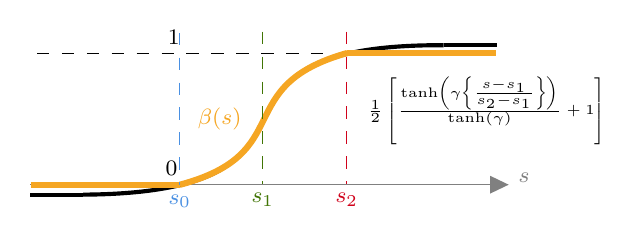
\begin{tikzpicture}[x=0.75pt,y=0.75pt,yscale=-1,xscale=1]
%uncomment if require: \path (0,215); %set diagram left start at 0, and has height of 215

%Straight Lines [id:da46631770507939163] 
\draw [color={rgb, 255:red, 128; green, 128; blue, 128 }  ,draw opacity=1 ]   (23,143.86) -- (250.5,143.86) ;
\draw [shift={(253.5,143.86)}, rotate = 180] [fill={rgb, 255:red, 128; green, 128; blue, 128 }  ,fill opacity=1 ][line width=0.08]  [draw opacity=0] (8.93,-4.29) -- (0,0) -- (8.93,4.29) -- cycle    ;
%Curve Lines [id:da39491275569940676] 
\draw [color={rgb, 255:red, 0; green, 0; blue, 0 }  ,draw opacity=1 ][line width=1.5]    (222.18,76.65) .. controls (87,76.16) and (185,147.66) .. (48.5,148.66) ;
%Straight Lines [id:da15611460318667292] 
\draw [color={rgb, 255:red, 0; green, 0; blue, 0 }  ,draw opacity=1 ][line width=1.5]    (23,148.66) -- (48.5,148.66) ;
%Straight Lines [id:da034171139038229326] 
\draw [color={rgb, 255:red, 0; green, 0; blue, 0 }  ,draw opacity=1 ][line width=1.5]    (222.18,76.65) -- (247.68,76.65) ;
%Straight Lines [id:da7075728897093001] 
\draw  [dash pattern={on 4.5pt off 4.5pt}]  (26.25,80.5) -- (247.25,80.5) ;
%Straight Lines [id:da5994500046428453] 
\draw [color={rgb, 255:red, 208; green, 2; blue, 27 }  ,draw opacity=1 ] [dash pattern={on 4.5pt off 4.5pt}]  (175.5,70.16) -- (175.5,143.41) ;
%Curve Lines [id:da28483688604328905] 
\draw [color={rgb, 255:red, 245; green, 166; blue, 35 }  ,draw opacity=1 ][line width=2.25]    (175.75,80.41) .. controls (119,96.41) and (152.25,128.66) .. (95,143.91) ;
%Straight Lines [id:da5305187515219363] 
\draw [color={rgb, 255:red, 245; green, 166; blue, 35 }  ,draw opacity=1 ][line width=2.25]    (175.75,80.41) -- (247.5,80.41) ;
%Straight Lines [id:da005336188299916778] 
\draw [color={rgb, 255:red, 245; green, 166; blue, 35 }  ,draw opacity=1 ][line width=2.25]    (23.25,143.91) -- (95,143.91) ;
%Straight Lines [id:da5146644196761871] 
\draw [color={rgb, 255:red, 65; green, 117; blue, 5 }  ,draw opacity=1 ] [dash pattern={on 4.5pt off 4.5pt}]  (135,70.16) -- (135,143.41) ;
%Straight Lines [id:da581762102800299] 
\draw [color={rgb, 255:red, 74; green, 144; blue, 226 }  ,draw opacity=1 ] [dash pattern={on 4.5pt off 4.5pt}]  (95,70.66) -- (95,143.91) ;

% Text Node
\draw (256.99,136.89) node [anchor=north west][inner sep=0.75pt]  [font=\footnotesize,color={rgb, 255:red, 128; green, 128; blue, 128 }  ,opacity=1 ]  {$s$};
% Text Node
\draw (114.25,118.76) node [anchor=south] [inner sep=0.75pt]  [font=\footnotesize,color={rgb, 255:red, 245; green, 166; blue, 35 }  ,opacity=1 ]  {$\beta ( s)$};
% Text Node
\draw (96.25,77.35) node [anchor=south east] [inner sep=0.75pt]  [font=\footnotesize]  {$1$};
% Text Node
\draw (95.19,140.6) node [anchor=south east] [inner sep=0.75pt]  [font=\footnotesize]  {$0$};
% Text Node
\draw (175.5,146.81) node [anchor=north] [inner sep=0.75pt]  [font=\footnotesize,color={rgb, 255:red, 208; green, 2; blue, 27 }  ,opacity=1 ]  {$s_{2}$};
% Text Node
\draw (184.07,108.31) node [anchor=west] [inner sep=0.75pt]  [font=\tiny,color={rgb, 255:red, 0; green, 0; blue, 0 }  ,opacity=1 ]  {$\frac{1}{2}\left[\frac{\tanh\left( \gamma \left\{\frac{s-s_{1}}{s_{2} -s_{1}}\right\}\right)}{\tanh( \gamma )} +1\right]$};
% Text Node
\draw (135,146.81) node [anchor=north] [inner sep=0.75pt]  [font=\footnotesize,color={rgb, 255:red, 65; green, 117; blue, 5 }  ,opacity=1 ]  {$s_{1}$};
% Text Node
\draw (95,147.31) node [anchor=north] [inner sep=0.75pt]  [font=\footnotesize,color={rgb, 255:red, 74; green, 144; blue, 226 }  ,opacity=1 ]  {$s_{0}$};


\end{tikzpicture}

            \caption{}
            \label{fig:transition:beta}
        \end{subfigure}
        \hfill
        \begin{subfigure}[b]{0.45\textwidth}
            \centering
            

\tikzset{every picture/.style={line width=0.75pt}} %set default line width to 0.75pt        

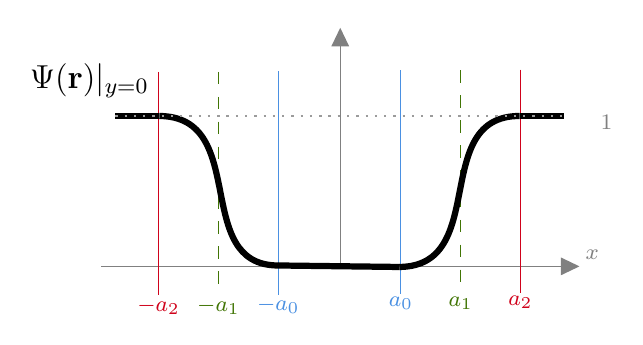
\begin{tikzpicture}[x=0.75pt,y=0.75pt,yscale=-1,xscale=1]
%uncomment if require: \path (0,216); %set diagram left start at 0, and has height of 216

%Straight Lines [id:da6021526004344566] 
\draw [color={rgb, 255:red, 128; green, 128; blue, 128 }  ,draw opacity=1 ]   (191.25,165.61) -- (191.25,53.66) ;
\draw [shift={(191.25,50.66)}, rotate = 90] [fill={rgb, 255:red, 128; green, 128; blue, 128 }  ,fill opacity=1 ][line width=0.08]  [draw opacity=0] (8.93,-4.29) -- (0,0) -- (8.93,4.29) -- cycle    ;
%Straight Lines [id:da09217173902055342] 
\draw [color={rgb, 255:red, 128; green, 128; blue, 128 }  ,draw opacity=1 ]   (76,165.61) -- (303.5,165.61) ;
\draw [shift={(306.5,165.61)}, rotate = 180] [fill={rgb, 255:red, 128; green, 128; blue, 128 }  ,fill opacity=1 ][line width=0.08]  [draw opacity=0] (8.93,-4.29) -- (0,0) -- (8.93,4.29) -- cycle    ;
%Straight Lines [id:da17327433842972684] 
\draw [color={rgb, 255:red, 74; green, 144; blue, 226 }  ,draw opacity=1 ]   (220.42,71.18) -- (220.42,178.87) ;
%Straight Lines [id:da5164207646575634] 
\draw [color={rgb, 255:red, 65; green, 117; blue, 5 }  ,draw opacity=1 ] [dash pattern={on 4.5pt off 4.5pt}]  (249.23,71.18) -- (249.23,178.87) ;
%Straight Lines [id:da9169226167412352] 
\draw [color={rgb, 255:red, 208; green, 2; blue, 27 }  ,draw opacity=1 ]   (278.04,70.82) -- (278.04,178.51) ;
%Straight Lines [id:da08965664307645271] 
\draw [color={rgb, 255:red, 208; green, 2; blue, 27 }  ,draw opacity=1 ]   (103.73,71.91) -- (103.73,179.59) ;
%Straight Lines [id:da855492609907931] 
\draw [color={rgb, 255:red, 65; green, 117; blue, 5 }  ,draw opacity=1 ] [dash pattern={on 4.5pt off 4.5pt}]  (132.54,71.91) -- (132.54,179.59) ;
%Straight Lines [id:da32654209361141806] 
\draw [color={rgb, 255:red, 74; green, 144; blue, 226 }  ,draw opacity=1 ]   (161.36,71.54) -- (161.36,179.23) ;
%Curve Lines [id:da03668323289068964] 
\draw [line width=2.25]    (104.09,93.15) .. controls (148.03,93.51) and (119.22,165.18) .. (161.36,165.18) ;
%Curve Lines [id:da11356455536917842] 
\draw [line width=2.25]    (277.68,93.15) .. controls (234.11,93.15) and (263.64,165.54) .. (219.7,165.9) ;
%Straight Lines [id:da3940509531593688] 
\draw [line width=2.25]    (161.36,165.18) -- (219.7,165.9) ;
%Straight Lines [id:da4374758728023367] 
\draw [line width=2.25]    (277.68,93.15) -- (298.93,93.15) ;
%Straight Lines [id:da7083449686833048] 
\draw [line width=2.25]    (82.84,93.15) -- (104.09,93.15) ;
%Straight Lines [id:da2928034275546325] 
\draw [color={rgb, 255:red, 155; green, 155; blue, 155 }  ,draw opacity=1 ][line width=0.75]  [dash pattern={on 0.84pt off 2.51pt}]  (82.84,93.15) -- (298,93.15) ;

% Text Node
\draw (308.24,156.39) node [anchor=north west][inner sep=0.75pt]  [font=\footnotesize,color={rgb, 255:red, 128; green, 128; blue, 128 }  ,opacity=1 ]  {$x$};
% Text Node
\draw (100.22,85.51) node [anchor=south east] [inner sep=0.75pt]  [font=\large,color={rgb, 255:red, 0; green, 0; blue, 0 }  ,opacity=1 ]  {$\Psi(\vec{r}) |_{y=0}$};
% Text Node
\draw (220.42,178.91) node [anchor=north] [inner sep=0.75pt]  [font=\footnotesize,color={rgb, 255:red, 74; green, 144; blue, 226 }  ,opacity=1 ]  {$a_{0}$};
% Text Node
\draw (249.23,178.91) node [anchor=north] [inner sep=0.75pt]  [font=\footnotesize,color={rgb, 255:red, 65; green, 117; blue, 5 }  ,opacity=1 ]  {$a_{1}$};
% Text Node
\draw (278.04,178.55) node [anchor=north] [inner sep=0.75pt]  [font=\footnotesize,color={rgb, 255:red, 208; green, 2; blue, 27 }  ,opacity=1 ]  {$a_{2}$};
% Text Node
\draw (161.36,179.27) node [anchor=north] [inner sep=0.75pt]  [font=\footnotesize,color={rgb, 255:red, 74; green, 144; blue, 226 }  ,opacity=1 ]  {$-a_{0}$};
% Text Node
\draw (132.54,179.63) node [anchor=north] [inner sep=0.75pt]  [font=\footnotesize,color={rgb, 255:red, 65; green, 117; blue, 5 }  ,opacity=1 ]  {$-a_{1}$};
% Text Node
\draw (103.73,179.63) node [anchor=north] [inner sep=0.75pt]  [font=\footnotesize,color={rgb, 255:red, 208; green, 2; blue, 27 }  ,opacity=1 ]  {$-a_{2}$};
% Text Node
\draw (319.5,100.76) node [anchor=south] [inner sep=0.75pt]  [font=\footnotesize,color={rgb, 255:red, 128; green, 128; blue, 128 }  ,opacity=1 ]  {$1$};


\end{tikzpicture}

            \caption{}
            \label{fig:transition:slice}
        \end{subfigure}
        \caption{(a) Curve of $\beta(s)$ in relation to $s_0$, $s_1$, and $s_2$. (b) Curve showing a slice of $\Psi$ on a placentone along $y = 0$ (i.e. on the basal plate) at the bottom of the cavity region, where $a_0$, $a_1$, and $a_2$ respectively denote the semi-minor axes of the inner, centre, and outer ellipses.}
        \label{fig:transition}
    \end{figure}

    The ellipses which form the geometry of the smooth transition region at the boundary of the central cavity are defined by
    \begin{align}
        \begin{split}
            r_0(\theta) & := \frac{a_0 b_0}{\sqrt{a_0^2 \sin^2(\theta) + b_0^2 \cos^2(\theta)}},
        \end{split}\\
        \begin{split}
            r_1(\theta) & := \frac{a_1 b_1}{\sqrt{a_1^2 \sin^2(\theta) + b_1^2 \cos^2(\theta)}},
        \end{split}\\
        \begin{split}
            r_2(\theta) & := \frac{a_2 b_2}{\sqrt{a_2^2 \sin^2(\theta) + b_2^2 \cos^2(\theta)}},
        \end{split}
    \end{align}
    where $\vec{x} \equiv (x, y)^\intercal$ are 2D Cartesian coordinates, and
    \begin{align}
        \begin{split}
            \theta(\vec{x}) & := \arctan{\left(\frac{y-c_2}{x-c_1}\right)},
        \end{split}\\
        \begin{split}
            r(\vec{x}) & := \sqrt{(\vec{x} - \vec{c}) \cdot (\vec{x} - \vec{c})}
        \end{split}
    \end{align}
    are 2D polar coordinates with $r = 0$ at $\vec{c} \equiv (c_1, c_2)^\intercal$ and $\theta = 0$ is tangential to the interface between $\Omega_\text{CC}$ and $\Omega_\text{a}$ (pointing in the anticlockwise direction). Here, $\vec{c}$ is the point at the centre of where an artery meets the placenta. The transition width, $\tau$, is defined such that $\tau = a_2 - a_0$ and $2\tau = b_2 - b_0$. The transition region in the central cavity is illustrated in Figure \ref{fig:transition-sizes:cavity}.

    \begin{figure}
        \begin{subfigure}[b]{0.45\textwidth}
            \centering
            

\tikzset{every picture/.style={line width=0.75pt}} %set default line width to 0.75pt        

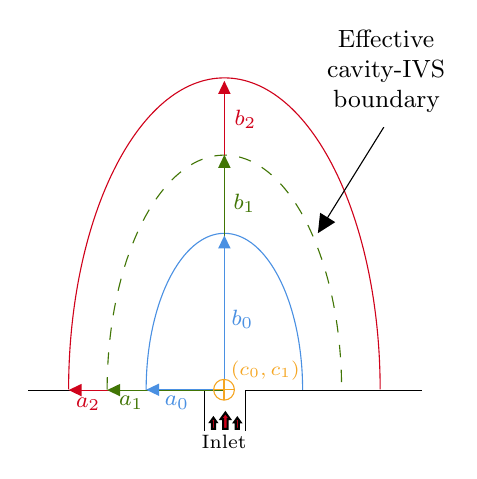
\begin{tikzpicture}[x=0.75pt,y=0.75pt,yscale=-1,xscale=1]
%uncomment if require: \path (0,300); %set diagram left start at 0, and has height of 300

%Shape: Arc [id:dp03766549009182518] 
\draw  [draw opacity=0] (43.89,241.51) .. controls (43.97,158.57) and (77.54,91.4) .. (118.94,91.4) .. controls (160.34,91.4) and (193.92,158.57) .. (194,241.51) -- (118.94,241.82) -- cycle ; \draw  [color={rgb, 255:red, 208; green, 2; blue, 27 }  ,draw opacity=1 ] (43.89,241.51) .. controls (43.97,158.57) and (77.54,91.4) .. (118.94,91.4) .. controls (160.34,91.4) and (193.92,158.57) .. (194,241.51) ;  
%Straight Lines [id:da2354434472901965] 
\draw    (109.5,241.82) -- (109.5,261.48) ;
%Straight Lines [id:da5144009246972279] 
\draw    (24.44,241.82) -- (108.75,241.82) ;
%Shape: Arc [id:dp18686074775091321] 
\draw  [draw opacity=0][dash pattern={on 4.5pt off 4.5pt}] (62.46,241.59) .. controls (62.52,179.17) and (87.79,128.62) .. (118.94,128.62) .. controls (150.1,128.62) and (175.36,179.17) .. (175.43,241.59) -- (118.94,241.82) -- cycle ; \draw  [color={rgb, 255:red, 65; green, 117; blue, 5 }  ,draw opacity=1 ][dash pattern={on 4.5pt off 4.5pt}] (62.46,241.59) .. controls (62.52,179.17) and (87.79,128.62) .. (118.94,128.62) .. controls (150.1,128.62) and (175.36,179.17) .. (175.43,241.59) ;  
%Shape: Arc [id:dp32870840671183665] 
\draw  [draw opacity=0] (81.25,241.66) .. controls (81.29,200.01) and (98.15,166.28) .. (118.94,166.28) .. controls (139.73,166.28) and (156.6,200.01) .. (156.64,241.66) -- (118.94,241.82) -- cycle ; \draw  [color={rgb, 255:red, 74; green, 144; blue, 226 }  ,draw opacity=1 ] (81.25,241.66) .. controls (81.29,200.01) and (98.15,166.28) .. (118.94,166.28) .. controls (139.73,166.28) and (156.6,200.01) .. (156.64,241.66) ;  
%Straight Lines [id:da13365761646036511] 
\draw [color={rgb, 255:red, 208; green, 2; blue, 27 }  ,draw opacity=1 ]   (118.94,241.82) -- (118.94,95.85) ;
\draw [shift={(118.94,92.85)}, rotate = 90] [fill={rgb, 255:red, 208; green, 2; blue, 27 }  ,fill opacity=1 ][line width=0.08]  [draw opacity=0] (6.25,-3) -- (0,0) -- (6.25,3) -- cycle    ;
%Straight Lines [id:da12333016540641895] 
\draw [color={rgb, 255:red, 208; green, 2; blue, 27 }  ,draw opacity=1 ]   (118.94,241.82) -- (46.89,241.82) ;
\draw [shift={(43.89,241.82)}, rotate = 360] [fill={rgb, 255:red, 208; green, 2; blue, 27 }  ,fill opacity=1 ][line width=0.08]  [draw opacity=0] (6.25,-3) -- (0,0) -- (6.25,3) -- cycle    ;
%Straight Lines [id:da33601944689998486] 
\draw [color={rgb, 255:red, 65; green, 117; blue, 5 }  ,draw opacity=1 ]   (118.94,241.82) -- (118.94,131.48) ;
\draw [shift={(118.94,128.48)}, rotate = 90] [fill={rgb, 255:red, 65; green, 117; blue, 5 }  ,fill opacity=1 ][line width=0.08]  [draw opacity=0] (6.25,-3) -- (0,0) -- (6.25,3) -- cycle    ;
%Straight Lines [id:da9639582332786008] 
\draw [color={rgb, 255:red, 65; green, 117; blue, 5 }  ,draw opacity=1 ]   (118.94,241.82) -- (65.46,241.82) ;
\draw [shift={(62.46,241.82)}, rotate = 360] [fill={rgb, 255:red, 65; green, 117; blue, 5 }  ,fill opacity=1 ][line width=0.08]  [draw opacity=0] (6.25,-3) -- (0,0) -- (6.25,3) -- cycle    ;
%Straight Lines [id:da29302727233729886] 
\draw [color={rgb, 255:red, 74; green, 144; blue, 226 }  ,draw opacity=1 ]   (118.78,241.66) -- (84.25,241.66) ;
\draw [shift={(81.25,241.66)}, rotate = 360] [fill={rgb, 255:red, 74; green, 144; blue, 226 }  ,fill opacity=1 ][line width=0.08]  [draw opacity=0] (6.25,-3) -- (0,0) -- (6.25,3) -- cycle    ;
%Straight Lines [id:da08146866090348959] 
\draw    (129.25,241.82) -- (214.25,241.82) ;
%Straight Lines [id:da2974174985117868] 
\draw    (129.25,241.82) -- (129.25,261.48) ;
%Straight Lines [id:da36914686722633006] 
\draw    (195.75,115.16) -- (165.58,163.68) ;
\draw [shift={(164,166.23)}, rotate = 301.87] [fill={rgb, 255:red, 0; green, 0; blue, 0 }  ][line width=0.08]  [draw opacity=0] (8.93,-4.29) -- (0,0) -- (8.93,4.29) -- cycle    ;
%Straight Lines [id:da06073675617036045] 
\draw [color={rgb, 255:red, 74; green, 144; blue, 226 }  ,draw opacity=1 ]   (118.94,241.82) -- (118.94,170.33) ;
\draw [shift={(118.94,167.33)}, rotate = 90] [fill={rgb, 255:red, 74; green, 144; blue, 226 }  ,fill opacity=1 ][line width=0.08]  [draw opacity=0] (6.25,-3) -- (0,0) -- (6.25,3) -- cycle    ;
%Flowchart: Or [id:dp5301694372224353] 
\draw  [color={rgb, 255:red, 245; green, 166; blue, 35 }  ,draw opacity=1 ] (113.78,241.66) .. controls (113.78,238.9) and (116.01,236.66) .. (118.78,236.66) .. controls (121.54,236.66) and (123.78,238.9) .. (123.78,241.66) .. controls (123.78,244.43) and (121.54,246.66) .. (118.78,246.66) .. controls (116.01,246.66) and (113.78,244.43) .. (113.78,241.66) -- cycle ; \draw  [color={rgb, 255:red, 245; green, 166; blue, 35 }  ,draw opacity=1 ] (113.78,241.66) -- (123.78,241.66) ; \draw  [color={rgb, 255:red, 245; green, 166; blue, 35 }  ,draw opacity=1 ] (118.78,236.66) -- (118.78,246.66) ;
%Right Arrow [id:dp5652546712623958] 
\draw  [fill={rgb, 255:red, 208; green, 2; blue, 27 }  ,fill opacity=1 ][line width=0.75]  (118.3,260.53) -- (118.3,255.8) -- (117.17,255.8) -- (119.42,252.66) -- (121.67,255.8) -- (120.54,255.8) -- (120.54,260.53) -- cycle ;
%Right Arrow [id:dp5523775393591213] 
\draw  [fill={rgb, 255:red, 208; green, 2; blue, 27 }  ,fill opacity=1 ][line width=0.75]  (112.88,260.51) -- (112.88,257.28) -- (112.11,257.28) -- (113.65,255.13) -- (115.18,257.28) -- (114.41,257.28) -- (114.41,260.51) -- cycle ;
%Right Arrow [id:dp3939210739992429] 
\draw  [fill={rgb, 255:red, 208; green, 2; blue, 27 }  ,fill opacity=1 ][line width=0.75]  (124.42,260.55) -- (124.42,257.33) -- (123.65,257.33) -- (125.18,255.18) -- (126.72,257.33) -- (125.95,257.33) -- (125.95,260.55) -- cycle ;

% Text Node
\draw (96.01,243.63) node [anchor=north] [inner sep=0.75pt]  [font=\footnotesize,color={rgb, 255:red, 74; green, 144; blue, 226 }  ,opacity=1 ]  {$a_{0}$};
% Text Node
\draw (74.01,243.63) node [anchor=north] [inner sep=0.75pt]  [font=\footnotesize,color={rgb, 255:red, 65; green, 117; blue, 5 }  ,opacity=1 ]  {$a_{1}$};
% Text Node
\draw (53.26,244.13) node [anchor=north] [inner sep=0.75pt]  [font=\footnotesize,color={rgb, 255:red, 208; green, 2; blue, 27 }  ,opacity=1 ]  {$a_{2}$};
% Text Node
\draw (121.12,207.93) node [anchor=west] [inner sep=0.75pt]  [font=\footnotesize,color={rgb, 255:red, 74; green, 144; blue, 226 }  ,opacity=1 ]  {$b_{0}$};
% Text Node
\draw (122.12,151.68) node [anchor=west] [inner sep=0.75pt]  [font=\footnotesize,color={rgb, 255:red, 65; green, 117; blue, 5 }  ,opacity=1 ]  {$b_{1}$};
% Text Node
\draw (122.62,111.43) node [anchor=west] [inner sep=0.75pt]  [font=\footnotesize,color={rgb, 255:red, 208; green, 2; blue, 27 }  ,opacity=1 ]  {$b_{2}$};
% Text Node
\draw (118.84,262.33) node [anchor=north] [inner sep=0.75pt]  [font=\Large] [align=left] {{\scriptsize Inlet}};
% Text Node
\draw (196.84,109.48) node [anchor=south] [inner sep=0.75pt]  [font=\small] [align=left] {\begin{minipage}[lt]{44.04pt}\setlength\topsep{0pt}
\begin{center}
Effective\\cavity-IVS\\boundary
\end{center}

\end{minipage}};
% Text Node
\draw (120.78,238.26) node [anchor=south west] [inner sep=0.75pt]  [font=\scriptsize,color={rgb, 255:red, 245; green, 166; blue, 35 }  ,opacity=1 ]  {$( c_{0} ,c_{1})$};


\end{tikzpicture}

            \caption{}
            \label{fig:transition-sizes:cavity}
        \end{subfigure}
        \hfill
        \begin{subfigure}[b]{0.45\textwidth}
            \centering
            

\tikzset{every picture/.style={line width=0.75pt}} %set default line width to 0.75pt        

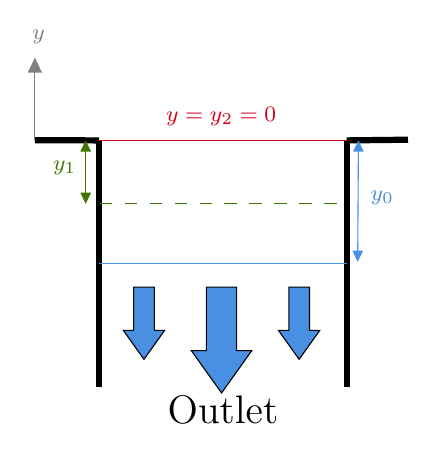
\begin{tikzpicture}[x=0.75pt,y=0.75pt,yscale=-1,xscale=1]
%uncomment if require: \path (0,232); %set diagram left start at 0, and has height of 232

%Straight Lines [id:da2544759348837675] 
\draw [line width=2.25]    (80.96,70) -- (80.96,188.66) ;
%Straight Lines [id:da7574547072545286] 
\draw [line width=2.25]    (200.22,188.66) -- (200.22,70) ;
%Straight Lines [id:da4990218087887346] 
\draw [line width=2.25]    (50,69.91) -- (80.96,70) ;
%Straight Lines [id:da5933583253972261] 
\draw [line width=2.25]    (200.22,70) -- (229.75,69.66) ;
%Straight Lines [id:da9214295287986949] 
\draw [color={rgb, 255:red, 208; green, 2; blue, 27 }  ,draw opacity=1 ]   (80.96,70) -- (200.22,70) ;
%Straight Lines [id:da1922898257916934] 
\draw [color={rgb, 255:red, 65; green, 117; blue, 5 }  ,draw opacity=1 ] [dash pattern={on 4.5pt off 4.5pt}]  (81.33,100.56) -- (200.59,100.56) ;
%Straight Lines [id:da7441027295861509] 
\draw [color={rgb, 255:red, 74; green, 144; blue, 226 }  ,draw opacity=1 ]   (80.96,129.33) -- (200.22,129.33) ;
%Straight Lines [id:da5144800892821806] 
\draw [color={rgb, 255:red, 74; green, 144; blue, 226 }  ,draw opacity=1 ]   (205.86,73) -- (205.53,125.51) ;
\draw [shift={(205.51,128.51)}, rotate = 270.36] [fill={rgb, 255:red, 74; green, 144; blue, 226 }  ,fill opacity=1 ][line width=0.08]  [draw opacity=0] (5.36,-2.57) -- (0,0) -- (5.36,2.57) -- cycle    ;
\draw [shift={(205.88,70)}, rotate = 90.36] [fill={rgb, 255:red, 74; green, 144; blue, 226 }  ,fill opacity=1 ][line width=0.08]  [draw opacity=0] (5.36,-2.57) -- (0,0) -- (5.36,2.57) -- cycle    ;
%Straight Lines [id:da9034738729177096] 
\draw [color={rgb, 255:red, 65; green, 117; blue, 5 }  ,draw opacity=1 ]   (74.46,73) -- (74.46,97.56) ;
\draw [shift={(74.46,100.56)}, rotate = 270] [fill={rgb, 255:red, 65; green, 117; blue, 5 }  ,fill opacity=1 ][line width=0.08]  [draw opacity=0] (5.36,-2.57) -- (0,0) -- (5.36,2.57) -- cycle    ;
\draw [shift={(74.46,70)}, rotate = 90] [fill={rgb, 255:red, 65; green, 117; blue, 5 }  ,fill opacity=1 ][line width=0.08]  [draw opacity=0] (5.36,-2.57) -- (0,0) -- (5.36,2.57) -- cycle    ;
%Straight Lines [id:da8984540196479969] 
\draw [color={rgb, 255:red, 128; green, 128; blue, 128 }  ,draw opacity=1 ]   (50,69.91) -- (50,33.16) ;
\draw [shift={(50,30.16)}, rotate = 90] [fill={rgb, 255:red, 128; green, 128; blue, 128 }  ,fill opacity=1 ][line width=0.08]  [draw opacity=0] (7.14,-3.43) -- (0,0) -- (7.14,3.43) -- cycle    ;
%Right Arrow [id:dp25345861768552247] 
\draw  [fill={rgb, 255:red, 74; green, 144; blue, 226 }  ,fill opacity=1 ] (147.21,140.66) -- (147.21,171.26) -- (154.5,171.26) -- (139.93,191.66) -- (125.36,171.26) -- (132.64,171.26) -- (132.64,140.66) -- cycle ;
%Right Arrow [id:dp07833670135680992] 
\draw  [fill={rgb, 255:red, 74; green, 144; blue, 226 }  ,fill opacity=1 ] (182.28,140.66) -- (182.28,161.54) -- (187.25,161.54) -- (177.3,175.47) -- (167.36,161.54) -- (172.33,161.54) -- (172.33,140.66) -- cycle ;
%Right Arrow [id:dp3532119282431716] 
\draw  [fill={rgb, 255:red, 74; green, 144; blue, 226 }  ,fill opacity=1 ] (107.53,140.66) -- (107.53,161.54) -- (112.5,161.54) -- (102.55,175.47) -- (92.61,161.54) -- (97.58,161.54) -- (97.58,140.66) -- cycle ;

% Text Node
\draw (210.54,97.74) node [anchor=west] [inner sep=0.75pt]  [font=\footnotesize,color={rgb, 255:red, 74; green, 144; blue, 226 }  ,opacity=1 ]  {$y_{0}$};
% Text Node
\draw (139.74,64.37) node [anchor=south] [inner sep=0.75pt]  [font=\footnotesize,color={rgb, 255:red, 208; green, 2; blue, 27 }  ,opacity=1 ]  {$y=y_{2} =0$};
% Text Node
\draw (71.2,83.22) node [anchor=east] [inner sep=0.75pt]  [font=\footnotesize,color={rgb, 255:red, 65; green, 117; blue, 5 }  ,opacity=1 ]  {$y_{1}$};
% Text Node
\draw (140.59,191.66) node [anchor=north] [inner sep=0.75pt]  [font=\Large] [align=left] {Outlet};
% Text Node
\draw (51.74,24.62) node [anchor=south] [inner sep=0.75pt]  [font=\footnotesize,color={rgb, 255:red, 128; green, 128; blue, 128 }  ,opacity=1 ]  {$y$};


\end{tikzpicture}

            \caption{}
            \label{fig:transition-sizes:vein}
        \end{subfigure}
        \caption{(a) Illustrates the semi-minor and semi-major axes defined in Appendix \ref{sec:smooth-transition} for the central cavity transition, including the marked point at the top of the centre of the inlet artery. (b) Illustrates parameters used in defining the smooth transition over the outlet veins.}
        \label{fig:transition-sizes}
    \end{figure}

    The smooth transition regions in the veins are defined using
    \begin{equation*}
        m(\vec{x}) := (\vec{x} - \vec{c}) \cdot \hat{\vec{n}},
    \end{equation*}
    where $\hat{\vec{n}} := \vec{n}/|\vec{n}|$, $\vec{n} = \vec{c} - \vec{p}$, and $\vec{p} \equiv (p_1, p_2)^\intercal$ is the centre of the large circle that traces out the curve on the basal plate. Here, $\vec{c}$ is the point at the centre of where a vein meets the placenta.

    The coefficient $\Psi$ is then given as
    \begin{equation}
        \Psi(\vec{x}) := 
        \begin{cases}
            0, & \text{if } \vec{x} \in \Omega_\text{a} \cup \Omega_\text{CC}, \\
            \beta_{r_0,r_1,r_2}(r(\vec{x})), & \text{if } \vec{x} \in \Omega_{\text{T}^-} \cup \Omega_{\text{T}^+}, \\
            \beta_{y_0,y_1,y_2}(m(\vec{x})), & \text{if } \vec{x} \in \Omega_\text{v}, \\
            1, & \text{if } \vec{x} \in \Omega_\text{IVS}, \\
        \end{cases}
        \label{eq:smooth-transition}
    \end{equation}
    where $y_2 - y_0$ is chosen to give a transition region in the veins with $y_1 \equiv \frac{y_0 + y_2}{2}$, which are shown in Figure \ref{fig:transition-sizes:vein}. A slice of $\Psi(\vec{x})$ on the placentone geometry along $y = 0$ is illustrated in Figure \ref{fig:transition:slice}.
    

    \chapter{Detailed comparison of flow models} \label{sec:flow-comparison}
    This appendix follows the results of \S\ref{sec:numerical-methods:blood-flow-experiments} and discusses them in more detail.

    On the 2D placentone simulations presented in Figure \ref{fig:4-models-placentone}, we immediately notice that the flow for S-B in Figure \ref{fig:4-models-placentone:s-b} is the only flow that does not exhibit recirculations in the central cavity. Figures \ref{fig:4-models-placentone:ns-b}--\ref{fig:4-models-placentone:nsb} have mostly similar behaviour. To see in which regions of the domains these models differ, we take differences of the solution on the placentone geometry for each combination of model (i.e. for models $i$ and $j$ respectively having velocity fields $\vec{u}_i$ and $\vec{u}_j$, we compute velocity magnitude using the usual Euclidean: $\norm{\vec{u}_i - \vec{u}_j}_{L^2(\Omega)}$). We will refer to these fields as `difference fields'. We study the difference fields only on the placentone geometry, as the differences in flow velocity are mostly localised to the arteries. The difference fields between all four velocity models are presented in Figure \ref{fig:4-models-placentone-norm-log}; note that the difference fields are visualised with a logarithmically-scaled colour scale, so differences may appear exaggerated. The difference fields involving S-B in Figures \ref{fig:4-models-placentone-norm-log:12}--\ref{fig:4-models-placentone-norm-log:14} are relatively large, especially in the central cavity region, but also in the upper section of the diverged artery. The difference field between NS-B and NS-NSD in Figure \ref{fig:4-models-placentone-norm-log:23} is the most subtle, with the difference largest in and above the veins, as well as a small amount on the cavity-IVS boundary. The difference fields involving NS-B and NS-NSD with NSD are respectively shown in Figures \ref{fig:4-models-placentone-norm-log:24} and \ref{fig:4-models-placentone-norm-log:34}, which are clearly similar due to NS-B and NS-NSD in themselves behaving similarly. We notice that the difference field in the artery is very small, and in fact small just above the artery, but grows larger further away from the artery mouth. Returning to Figure \ref{fig:4-models-placentone}, we can see the centre of the recirculation zones for NSD sit closer to the artery than those shown for NS-B and NS-NSD, therefore increasing the value in the difference field in the cavity here; this effect is also likely sensitive to the chosen cavity transition, $\tau$.

    \begin{figure}
        \thisfloatpagestyle{empty}
        % GENERATED WITH MONOLITH COMMIT: XXX
        % GENERATED ON 2024-XX-XX
        \centering
        \begin{subfigure}[b]{0.45\textwidth}
            \centering
            \includegraphics[width=\textwidth]{diagrams/results-modelling/velocity-transport/meshandsoln_dg_velocity_placentone_nsb_velocity-log.png}
            \caption{}
        \end{subfigure}
        \hfill
        \begin{subfigure}[b]{0.45\textwidth}
            \centering
            \includegraphics[width=\textwidth]{diagrams/results-modelling/velocity-transport/meshandsoln_dg_velocity_placentone_s-b_velocity-log.png}
            \caption{}
        \end{subfigure}
        \begin{subfigure}[b]{0.45\textwidth}
            \centering
            \includegraphics[width=\textwidth]{diagrams/results-modelling/velocity-transport/meshandsoln_dg_velocity_placentone_ns-b_velocity-log.png}
            \caption{}
        \end{subfigure}
        \hfill
        \begin{subfigure}[b]{0.45\textwidth}
            \centering
            \includegraphics[width=\textwidth]{diagrams/results-modelling/velocity-transport/meshandsoln_dg_velocity_placentone_ns-nsb_velocity-log.png}
            \caption{}
        \end{subfigure}
        \figureretag{fig:4-models-placentone}
        \caption{Velocity plot on placentone geometry, with logarithmically-scaled velocity colouring and streamlines shown in black for (a) NSD (Equation \eqref{eq:nsb}), (b) S-B (Equation \eqref{eq:s-b}), (c) NS-B (Equation \eqref{eq:ns-b}), and (d) NS-NSD (Equation \eqref{eq:ns-nsb}).}
    \end{figure}

    To make a quantitative comparison, we also compute the $L^2$-norm between each combination of solutions. That is to say, for velocity fields $\vec{u}_i$ and $\vec{u}_j$, we compute
    \begin{equation}
        \norm{\vec{u}_i - \vec{u}_j}_{L^2(\Omega)} := \sqrt{\int_\Omega (\vec{u}_i - \vec{u}_j) \cdot (\vec{u}_i - \vec{u}_j) \diff \vec{x}}.
    \end{equation}
    These norms are given in Table \ref{tab:4-models-placentone-l2}. We notice that the largest norms are between the differences involving S-B, which likely is contributed to by the lack of recirculations with S-B. The smallest norm is between NS-B and NS-NSD, showing that these equations exhibit the most similar fluid flow. This overall shows us quantitatively that all four models are `close' under the $L^2$-norm, and agrees with the qualitative comparisons we made in \S\ref{sec:numerical-methods:blood-flow-experiments:comparison}. 

    \begin{figure}
        % GENERATED WITH MONOLITH COMMIT: XXX
        % GENERATED ON 2024-XX-XX AT XX:XX
        \begin{subfigure}[b]{0.3\textwidth}
            \centering
            \includegraphics[width=\textwidth]{diagrams/results-modelling/velocity-comparison/meshandsoln_dg_velocity_placentone_14_velocity-log.png}
            \caption{}
            \label{fig:4-models-placentone-norm-log:14}
        \end{subfigure}
        \hfill
        \begin{subfigure}[b]{0.3\textwidth}
            \centering
            \includegraphics[width=\textwidth]{diagrams/results-modelling/velocity-comparison/meshandsoln_dg_velocity_placentone_24_velocity-log.png}
            \caption{}
            \label{fig:4-models-placentone-norm-log:24}
        \end{subfigure}
        \hfill
        \begin{subfigure}[b]{0.3\textwidth}
            \centering
            \includegraphics[width=\textwidth]{diagrams/results-modelling/velocity-comparison/meshandsoln_dg_velocity_placentone_34_velocity-log.png}
            \caption{}
            \label{fig:4-models-placentone-norm-log:34}
        \end{subfigure}
        \begin{subfigure}[b]{0.3\textwidth}
            \centering
            \includegraphics[width=\textwidth]{diagrams/results-modelling/velocity-comparison/meshandsoln_dg_velocity_placentone_12_velocity-log.png}
            \caption{}
            \label{fig:4-models-placentone-norm-log:12}
        \end{subfigure}
        \hfill
        \begin{subfigure}[b]{0.3\textwidth}
            \centering
            \includegraphics[width=\textwidth]{diagrams/results-modelling/velocity-comparison/meshandsoln_dg_velocity_placentone_13_velocity-log.png}
            \caption{}
            \label{fig:4-models-placentone-norm-log:13}
        \end{subfigure}
        \hfill
        \begin{subfigure}[b]{0.3\textwidth}
            \centering
            \includegraphics[width=\textwidth]{diagrams/results-modelling/velocity-comparison/meshandsoln_dg_velocity_placentone_23_velocity-log.png}
            \caption{}
            \label{fig:4-models-placentone-norm-log:23}
        \end{subfigure}            

        \caption{Difference fields on a placentone, visualised with a logarithmic colour scaling. Differences are computed between approximations to (a) NSD and S-B (Equations \eqref{eq:nsb} and \eqref{eq:s-b}), (b) NSD and NS-B (Equations \eqref{eq:nsb} and \eqref{eq:ns-b}), (c) NSD and NS-NSD (Equations \eqref{eq:nsb} and \eqref{eq:ns-nsb}), (d) S-B and NS-B (Equations \eqref{eq:s-b} and \eqref{eq:ns-b}), (e) S-B and NS-NSD (Equations \eqref{eq:s-b} and \eqref{eq:ns-nsb}), and (f) NS-B and NS-NSD (Equations \eqref{eq:ns-b} and \eqref{eq:ns-nsb}).}
        \label{fig:4-models-placentone-norm-log}
    \end{figure}

    \begin{table}[]
        % GENERATED WITH MONOLITH COMMIT: 0a636bb668309760e0d5884a4fe4684931582d11
        % GENERATED ON 2024-01-12 AT 10:45
        \centering
        \begin{tabular}{c|cccc}
              & S-B & NS-B & NS-NSD & NSD \\
             \hline
             S-B (Equation \eqref{eq:s-b}) & \num{0} & - & - & - \\
             NS-B (Equation \eqref{eq:ns-b}) & \num{1.32E-02} & \num{0} & - & - \\
             NS-NSD (Equation \eqref{eq:ns-nsb}) & \num{1.31E-02} & \num{1.83E-04} & \num{0} & - \\
             NSD (Equation \eqref{eq:nsb}) & \num{8.43E-03} & \num{8.71E-03} & \num{8.69E-03} & \num{0} 
        \end{tabular}
        \caption{$L_2$-norm of solutions on the placentone geometry using each combination of the four velocity models.}
        \label{tab:4-models-placentone-l2}
    \end{table}

    \chapter{Lax-Friedrichs flux \texorpdfstring{$\alpha$}{α} parameter} \label{sec:lax-friedrichs}
    We will derive the $\alpha$ parameter used in the modified Lax-Friedrichs flux in Equation \eqref{eq:lax-friedrichs-modified}; a similar procedure may be followed for the standard Lax-Friedrichs flux in Equation \eqref{eq:lax-friedrichs} by selecting $\vec{w} \equiv \vec{0}$.
    
    The Lax-Friedrichs flux used in Chapter \ref{sec:contractions}, $\bar{\mathcal{H}}$, is defined in Equation \ref{eq:lax-friedrichs-modified}; $\bar{\mathcal{H}}$ is a numerical flux function that approximates $(\vec{u} \otimes [\vec{u} - \vec{w}]) \cdot \vec{n}$. To help the reader, we rewrite these equations below:
    \begin{equation}
        \bar{\mathcal{H}}_\text{f}(\vec{u}^+, \vec{u}_\Gamma, \vec{n}; \vec{w}) := \frac{1}{2} ((\vec{u}^+ \otimes [\vec{u}^+ - \vec{w}]) \cdot \vec{n} + (\vec{u}_\Gamma \otimes [\vec{u}_\Gamma - \vec{w}]) \cdot \vec{n} + (\alpha \vec{u}^+ - \alpha \vec{u}_\Gamma)),
        \tag{\ref{eq:lax-friedrichs-modified} repeated}
    \end{equation}
    where 
    \begin{equation}
        \vec{u}_\Gamma := 
        \begin{cases}
        \vec{u}^- & \text{on~} \mathcal{F}^\mathcal{I}, \\
            \vec{u}^+ & \text{on~} \Gamma_N, \\
            \vec{g}_D & \text{on~} \Gamma_D, 
        \end{cases}
        \tag{\ref{eq:u_gamma} repeated}
    \end{equation}
    and $\alpha$ is an estimate of the largest eigenvalue (in absolute value) of the following Jacobi matrix in the neighbourhood of the boundary of the element it is computed on (i.e. $\partial \kappa$) \cite{hartmannAdaptiveDiscontinuousGalerkin2003}:
    \begin{equation*}
        \pdv{}{\vec{u}}\left[ (\vec{u} \otimes [\vec{u} - \vec{w}]) \cdot \vec{n} \right].
    \end{equation*}

    Writing $\vec{u} \equiv (u_1, u_2)^\intercal$, $\vec{n} \equiv (n_1, n_2)^\intercal$, and $\vec{w} \equiv (w_1, w_2)^\intercal$, we have
    \begin{align*}
        (\vec{u} \otimes [\vec{u} - \vec{w}]) \cdot \vec{n} & \equiv
        \begin{bmatrix}
            u_1 (u_1 - w_1) & u_1 (u_2 - w_2) \\
            u_2 (u_1 - w_1) & u_2 (u_2 - w_2)
        \end{bmatrix}
        \begin{bmatrix}
            n_1 \\
            n_2
        \end{bmatrix}.
    \end{align*}

    Taking the derivative with respect to $\vec{u}$ gives
    \begin{equation*}
        \pdv{}{\vec{u}}\left[ (\vec{u} \otimes [\vec{u} - \vec{w}]) \cdot \vec{n} \right] \equiv \begin{bmatrix}
            u_1n_2 + (\vec{u} - \vec{w}) \cdot \vec{n} & u_1n_2 \\
            u_2n_1 & u_2n_2 + (\vec{u} - \vec{w}) \cdot \vec{n}
        \end{bmatrix}
    \end{equation*}
    for which the eigenvalues are $2\vec{u} \cdot \vec{n} - \vec{w}\cdot\vec{n}$ and $\vec{u} \cdot \vec{n} - \vec{w}\cdot\vec{n}$; therefore, we obtain
    \begin{equation}
        \alpha = \max(|2\vec{u}^+\cdot\vec{n} - \vec{w} \cdot \vec{n}|, |2\vec{u}_\Gamma\cdot\vec{n} - \vec{w} \cdot \vec{n}|, |\vec{u}^+ \cdot \vec{n} - \vec{w} \cdot \vec{n}|, |\vec{u}_\Gamma \cdot \vec{n} - \vec{w} \cdot \vec{n}|).
        \retag{eq:lf-alpha-velocity}
    \end{equation}

    % \chapter{Derivation of \texorpdfstring{$\Phi$}{Φ}} \label{sec:analytical-energy}
    \todoitemone{$R$ used here, $r$ used elsewhere}
    
    Here, we outline the derivation of $\Phi$, which is used in \S\ref{sec:nutrient-uptake:variation-of-vessels} as the approximation
    \begin{equation*}
        \Phi(N_\text{A}, N_\text{V}) \approx \frac{E_\text{kinetic}(\Gamma_\text{in}) - E_\text{kinetic}(\Gamma_\text{out})}{E_\text{kinetic}(\Gamma_\text{in})}.
    \end{equation*}

    We begin by considering Figure \ref{fig:analytical-expression-placenta}, which shows a simplified view of the inlets and outlets in the placenta, which has $N_\text{A}$ arteries, $N_\text{V}$ basal plate and septal wall veins, and $2$ marginal sinus veins; this reflects the problem setup throughout \S\ref{sec:nutrient-uptake:variation-of-vessels}. The flux of blood, $Q$, through each inlet and outlet is calculated as
    \begin{equation}
        Q = \frac{4 U R}{3},
    \end{equation}
    where we have assumed a Poiseuille flow of peak $U$ and radius $R$. The peak inflow speeds for the arteries are given as $\{ U_{\text{in},1}, ..., U_{\text{in},N_\text{A}} \}$ with artery radius $R_\text{a}$, therefore giving fluxes $$Q_\text{in} := \{ U_{\text{in},j} R_\text{A} \}_j.$$ Similarly, fluxes through the basal plate and septal wall veins are given as $$Q_\text{out} := \{ U_{\text{out},j} R_\text{V} \}_j,$$ and fluxes through marginal sinus veins are given as $$\{ Q^\text{ms}_\text{out} := U^\text{ms}_{\text{out},1} R^\text{ms}_\text{V}, U^\text{ms}_{\text{out},2} R^\text{ms}_\text{V} \}.$$
    
    \begin{figure}
        \centering
        

\tikzset{every picture/.style={line width=0.75pt}} %set default line width to 0.75pt        

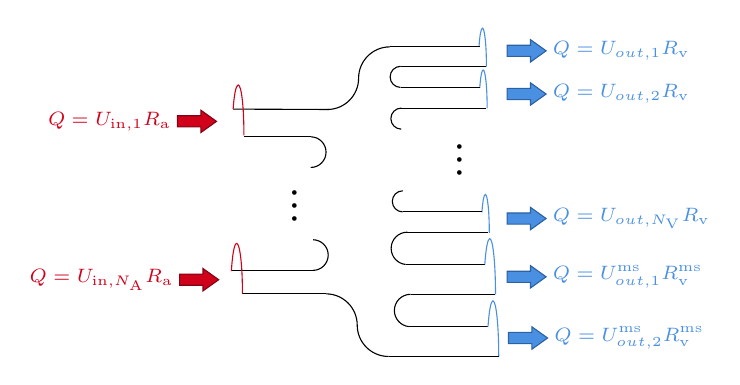
\begin{tikzpicture}[x=0.75pt,y=0.75pt,yscale=-1,xscale=1]
%uncomment if require: \path (0,300); %set diagram left start at 0, and has height of 300

%Straight Lines [id:da6897475479741801] 
\draw    (182.17,71.91) -- (228.6,72.09) ;
%Straight Lines [id:da9207632072413952] 
\draw    (187.34,85.27) -- (219.69,85.27) ;
%Shape: Arc [id:dp5144902494751977] 
\draw  [draw opacity=0] (242.63,57) .. controls (242.63,65.33) and (235.88,72.09) .. (227.56,72.09) -- (227.55,57.01) -- cycle ; \draw   (242.63,57) .. controls (242.63,65.33) and (235.88,72.09) .. (227.56,72.09) ;  
%Shape: Arc [id:dp044092686186237184] 
\draw  [draw opacity=0] (242.63,57) .. controls (242.63,48.67) and (249.38,41.92) .. (257.71,41.92) -- (257.71,57) -- cycle ; \draw   (242.63,57) .. controls (242.63,48.67) and (249.38,41.92) .. (257.71,41.92) ;  
%Straight Lines [id:da7127120437770351] 
\draw    (257.71,41.92) -- (301.07,41.92) ;
%Straight Lines [id:da36592894326131375] 
\draw    (262.91,51.29) -- (303.82,51.29) ;
%Shape: Arc [id:dp8073218791002419] 
\draw  [draw opacity=0] (262.82,61.46) .. controls (260.05,61.41) and (257.82,59.15) .. (257.82,56.37) .. controls (257.82,53.56) and (260.1,51.29) .. (262.91,51.29) -- (262.91,56.37) -- cycle ; \draw   (262.82,61.46) .. controls (260.05,61.41) and (257.82,59.15) .. (257.82,56.37) .. controls (257.82,53.56) and (260.1,51.29) .. (262.91,51.29) ;  
%Shape: Arc [id:dp9115427482667546] 
\draw  [draw opacity=0] (257.04,191.08) .. controls (248.71,191.08) and (241.96,184.32) .. (241.96,175.99) -- (257.04,175.99) -- cycle ; \draw   (257.04,191.08) .. controls (248.71,191.08) and (241.96,184.32) .. (241.96,175.99) ;  
%Shape: Arc [id:dp40739579709299334] 
\draw  [draw opacity=0] (226.88,160.91) .. controls (235.2,160.91) and (241.96,167.67) .. (241.96,175.99) -- (226.88,175.99) -- cycle ; \draw   (226.88,160.91) .. controls (235.2,160.91) and (241.96,167.67) .. (241.96,175.99) ;  
%Straight Lines [id:da315564227105416] 
\draw    (186.63,160.91) -- (226.88,160.91) ;
%Shape: Arc [id:dp06802366651187608] 
\draw  [draw opacity=0] (220.73,134.85) .. controls (224.75,134.92) and (227.98,138.2) .. (227.98,142.23) .. controls (227.98,146.3) and (224.68,149.61) .. (220.61,149.61) -- (220.61,142.23) -- cycle ; \draw   (220.73,134.85) .. controls (224.75,134.92) and (227.98,138.2) .. (227.98,142.23) .. controls (227.98,146.3) and (224.68,149.61) .. (220.61,149.61) ;  
%Straight Lines [id:da27217516789748486] 
\draw    (181.45,149.61) -- (220.61,149.61) ;
%Shape: Arc [id:dp1353432404024142] 
\draw  [draw opacity=0] (219.69,85.27) .. controls (223.71,85.33) and (226.94,88.61) .. (226.94,92.64) .. controls (226.94,96.72) and (223.64,100.02) .. (219.57,100.02) -- (219.57,92.64) -- cycle ; \draw   (219.69,85.27) .. controls (223.71,85.33) and (226.94,88.61) .. (226.94,92.64) .. controls (226.94,96.72) and (223.64,100.02) .. (219.57,100.02) ;  
%Shape: Arc [id:dp238698053685636] 
\draw  [draw opacity=0] (182.17,71.91) .. controls (182.66,64.96) and (183.56,60.28) .. (184.6,60.28) .. controls (186.13,60.28) and (187.37,70.68) .. (187.36,83.51) .. controls (187.36,83.85) and (187.35,84.19) .. (187.35,84.52) -- (184.57,83.51) -- cycle ; \draw  [color={rgb, 255:red, 208; green, 2; blue, 27 }  ,draw opacity=1 ] (182.17,71.91) .. controls (182.66,64.96) and (183.56,60.28) .. (184.6,60.28) .. controls (186.13,60.28) and (187.37,70.68) .. (187.36,83.51) .. controls (187.36,83.85) and (187.35,84.19) .. (187.35,84.52) ;  
%Shape: Arc [id:dp8213186661755791] 
\draw  [draw opacity=0] (181.34,150.01) .. controls (181.79,142.1) and (182.76,136.62) .. (183.87,136.62) .. controls (185.41,136.62) and (186.65,147.02) .. (186.64,159.85) .. controls (186.63,160.19) and (186.63,160.53) .. (186.63,160.86) -- (183.85,159.85) -- cycle ; \draw  [color={rgb, 255:red, 208; green, 2; blue, 27 }  ,draw opacity=1 ] (181.34,150.01) .. controls (181.79,142.1) and (182.76,136.62) .. (183.87,136.62) .. controls (185.41,136.62) and (186.65,147.02) .. (186.64,159.85) .. controls (186.63,160.19) and (186.63,160.53) .. (186.63,160.86) ;  
%Shape: Arc [id:dp20383419320801943] 
\draw  [draw opacity=0] (300.66,41.52) .. controls (301.01,36.36) and (301.61,32.94) .. (302.3,32.94) .. controls (303.36,32.94) and (304.22,41.22) .. (304.21,51.44) -- (302.28,51.47) -- cycle ; \draw  [color={rgb, 255:red, 74; green, 144; blue, 226 }  ,draw opacity=1 ] (300.66,41.52) .. controls (301.01,36.36) and (301.61,32.94) .. (302.3,32.94) .. controls (303.36,32.94) and (304.22,41.22) .. (304.21,51.44) ;  
%Straight Lines [id:da9273006738288603] 
\draw    (263.26,71.4) -- (304.17,71.4) ;
%Shape: Arc [id:dp20008369967725814] 
\draw  [draw opacity=0] (263.17,81.57) .. controls (260.4,81.52) and (258.17,79.26) .. (258.17,76.48) .. controls (258.17,73.67) and (260.45,71.4) .. (263.26,71.4) -- (263.26,76.48) -- cycle ; \draw   (263.17,81.57) .. controls (260.4,81.52) and (258.17,79.26) .. (258.17,76.48) .. controls (258.17,73.67) and (260.45,71.4) .. (263.26,71.4) ;  
%Shape: Arc [id:dp8626799595145647] 
\draw  [draw opacity=0] (301.01,61.63) .. controls (301.35,56.47) and (301.96,53.05) .. (302.64,53.05) .. controls (303.71,53.05) and (304.56,61.33) .. (304.56,71.55) -- (302.63,71.58) -- cycle ; \draw  [color={rgb, 255:red, 74; green, 144; blue, 226 }  ,draw opacity=1 ] (301.01,61.63) .. controls (301.35,56.47) and (301.96,53.05) .. (302.64,53.05) .. controls (303.71,53.05) and (304.56,61.33) .. (304.56,71.55) ;  
%Straight Lines [id:da0589129492536995] 
\draw    (262.82,61.46) -- (301.01,61.46) ;
%Straight Lines [id:da30421383578476013] 
\draw    (264.3,131.38) -- (305.21,131.38) ;
%Shape: Arc [id:dp200178610381043] 
\draw  [draw opacity=0] (265.25,146.76) .. controls (261.35,146.33) and (258.31,143.02) .. (258.31,139) .. controls (258.31,134.69) and (261.8,131.2) .. (266.11,131.2) -- (266.11,139) -- cycle ; \draw   (265.25,146.76) .. controls (261.35,146.33) and (258.31,143.02) .. (258.31,139) .. controls (258.31,134.69) and (261.8,131.2) .. (266.11,131.2) ;  
%Shape: Arc [id:dp4498403889935414] 
\draw  [draw opacity=0] (302.05,121.62) .. controls (302.39,116.46) and (303,113.04) .. (303.68,113.04) .. controls (304.75,113.04) and (305.6,121.32) .. (305.6,131.54) -- (303.67,131.57) -- cycle ; \draw  [color={rgb, 255:red, 74; green, 144; blue, 226 }  ,draw opacity=1 ] (302.05,121.62) .. controls (302.39,116.46) and (303,113.04) .. (303.68,113.04) .. controls (304.75,113.04) and (305.6,121.32) .. (305.6,131.54) ;  
%Straight Lines [id:da22468899311040502] 
\draw    (263.86,121.44) -- (302.05,121.44) ;
%Shape: Arc [id:dp19536738802800802] 
\draw  [draw opacity=0] (263.86,121.44) .. controls (261.09,121.4) and (258.86,119.14) .. (258.86,116.36) .. controls (258.86,113.55) and (261.14,111.27) .. (263.95,111.27) -- (263.95,116.36) -- cycle ; \draw   (263.86,121.44) .. controls (261.09,121.4) and (258.86,119.14) .. (258.86,116.36) .. controls (258.86,113.55) and (261.14,111.27) .. (263.95,111.27) ;  
%Straight Lines [id:da522381672409731] 
\draw    (265.25,146.76) -- (303.43,146.76) ;
%Shape: Arc [id:dp7499727362361837] 
\draw  [draw opacity=0] (303.43,146.76) .. controls (303.94,139.28) and (304.81,134.32) .. (305.81,134.32) .. controls (307.35,134.32) and (308.59,146.32) .. (308.58,161.14) -- (305.78,161.19) -- cycle ; \draw  [color={rgb, 255:red, 74; green, 144; blue, 226 }  ,draw opacity=1 ] (303.43,146.76) .. controls (303.94,139.28) and (304.81,134.32) .. (305.81,134.32) .. controls (307.35,134.32) and (308.59,146.32) .. (308.58,161.14) ;  
%Straight Lines [id:da4989617610080148] 
\draw    (267.66,161.14) -- (308.58,161.14) ;
%Shape: Arc [id:dp47436356415299286] 
\draw  [draw opacity=0] (266.8,176.69) .. controls (262.9,176.26) and (259.86,172.96) .. (259.86,168.94) .. controls (259.86,164.63) and (263.35,161.14) .. (267.66,161.14) -- (267.66,168.94) -- cycle ; \draw   (266.8,176.69) .. controls (262.9,176.26) and (259.86,172.96) .. (259.86,168.94) .. controls (259.86,164.63) and (263.35,161.14) .. (267.66,161.14) ;  
%Straight Lines [id:da47731005062437015] 
\draw    (266.8,176.69) -- (304.98,176.69) ;
%Shape: Arc [id:dp6764201761859778] 
\draw  [draw opacity=0] (304.98,176.69) .. controls (305.49,169.22) and (306.36,164.26) .. (307.35,164.26) .. controls (308.9,164.26) and (310.14,176.26) .. (310.13,191.08) -- (307.33,191.13) -- cycle ; \draw  [color={rgb, 255:red, 74; green, 144; blue, 226 }  ,draw opacity=1 ] (304.98,176.69) .. controls (305.49,169.22) and (306.36,164.26) .. (307.35,164.26) .. controls (308.9,164.26) and (310.14,176.26) .. (310.13,191.08) ;  
%Straight Lines [id:da8107752914505761] 
\draw    (257.04,191.08) -- (310.13,191.08) ;
%Right Arrow [id:dp2469458095146153] 
\draw  [color={rgb, 255:red, 129; green, 4; blue, 20 }  ,draw opacity=1 ][fill={rgb, 255:red, 208; green, 2; blue, 27 }  ,fill opacity=1 ] (155.35,75.12) -- (166.64,75.12) -- (166.64,72.44) -- (174.16,77.81) -- (166.64,83.19) -- (166.64,80.5) -- (155.35,80.5) -- cycle ;
%Right Arrow [id:dp9958402750896171] 
\draw  [color={rgb, 255:red, 44; green, 97; blue, 162 }  ,draw opacity=1 ][fill={rgb, 255:red, 74; green, 144; blue, 226 }  ,fill opacity=1 ] (314.16,41.14) -- (325.45,41.14) -- (325.45,38.46) -- (332.97,43.83) -- (325.45,49.21) -- (325.45,46.52) -- (314.16,46.52) -- cycle ;
%Right Arrow [id:dp6128543836231557] 
\draw  [color={rgb, 255:red, 44; green, 97; blue, 162 }  ,draw opacity=1 ][fill={rgb, 255:red, 74; green, 144; blue, 226 }  ,fill opacity=1 ] (314.16,61.95) -- (325.45,61.95) -- (325.45,59.26) -- (332.97,64.64) -- (325.45,70.01) -- (325.45,67.32) -- (314.16,67.32) -- cycle ;
%Right Arrow [id:dp7930204983840552] 
\draw  [color={rgb, 255:red, 44; green, 97; blue, 162 }  ,draw opacity=1 ][fill={rgb, 255:red, 74; green, 144; blue, 226 }  ,fill opacity=1 ] (314.16,121.94) -- (325.45,121.94) -- (325.45,119.25) -- (332.97,124.62) -- (325.45,130) -- (325.45,127.31) -- (314.16,127.31) -- cycle ;
%Right Arrow [id:dp8020822248149451] 
\draw  [color={rgb, 255:red, 44; green, 97; blue, 162 }  ,draw opacity=1 ][fill={rgb, 255:red, 74; green, 144; blue, 226 }  ,fill opacity=1 ] (314.16,150.02) -- (325.45,150.02) -- (325.45,147.33) -- (332.97,152.71) -- (325.45,158.08) -- (325.45,155.4) -- (314.16,155.4) -- cycle ;
%Right Arrow [id:dp05601739812042572] 
\draw  [color={rgb, 255:red, 44; green, 97; blue, 162 }  ,draw opacity=1 ][fill={rgb, 255:red, 74; green, 144; blue, 226 }  ,fill opacity=1 ] (314.86,179.49) -- (326.14,179.49) -- (326.14,176.81) -- (333.67,182.18) -- (326.14,187.56) -- (326.14,184.87) -- (314.86,184.87) -- cycle ;
%Right Arrow [id:dp45340586186745924] 
\draw  [color={rgb, 255:red, 129; green, 4; blue, 20 }  ,draw opacity=1 ][fill={rgb, 255:red, 208; green, 2; blue, 27 }  ,fill opacity=1 ] (156.39,151.41) -- (167.68,151.41) -- (167.68,148.72) -- (175.21,154.1) -- (167.68,159.47) -- (167.68,156.78) -- (156.39,156.78) -- cycle ;

% Text Node
\draw (291.46,96.24) node  [font=\LARGE,rotate=-90]  {$...$};
% Text Node
\draw (211.77,118.4) node  [font=\LARGE,rotate=-90]  {$...$};
% Text Node
\draw (153.35,77.81) node [anchor=east] [inner sep=0.75pt]  [font=\scriptsize,color={rgb, 255:red, 208; green, 2; blue, 27 }  ,opacity=1 ]  {$Q=U_{\text{in} ,1} R_{\text{a}}$};
% Text Node
\draw (154.39,154.1) node [anchor=east] [inner sep=0.75pt]  [font=\scriptsize,color={rgb, 255:red, 208; green, 2; blue, 27 }  ,opacity=1 ]  {$Q=U_{\text{in} ,N_{\text{A}}} R_{\text{a}}$};
% Text Node
\draw (334.97,43.83) node [anchor=west] [inner sep=0.75pt]  [font=\scriptsize,color={rgb, 255:red, 74; green, 144; blue, 226 }  ,opacity=1 ]  {$Q=U_{out,1} R_{\text{v}}$};
% Text Node
\draw (334.97,64.64) node [anchor=west] [inner sep=0.75pt]  [font=\scriptsize,color={rgb, 255:red, 74; green, 144; blue, 226 }  ,opacity=1 ]  {$Q=U_{out,2} R_{\text{v}}$};
% Text Node
\draw (334.97,124.62) node [anchor=west] [inner sep=0.75pt]  [font=\scriptsize,color={rgb, 255:red, 74; green, 144; blue, 226 }  ,opacity=1 ]  {$Q=U_{out,N_{\text{V}}} R_{\text{v}}$};
% Text Node
\draw (334.97,152.71) node [anchor=west] [inner sep=0.75pt]  [font=\scriptsize,color={rgb, 255:red, 74; green, 144; blue, 226 }  ,opacity=1 ]  {$Q=U_{out,1}^{\text{ms}} R_{\text{v}}^{\text{ms}}$};
% Text Node
\draw (335.67,182.18) node [anchor=west] [inner sep=0.75pt]  [font=\scriptsize,color={rgb, 255:red, 74; green, 144; blue, 226 }  ,opacity=1 ]  {$Q=U_{out,2}^{\text{ms}} R_{\text{v}}^{\text{ms}}$};


\end{tikzpicture}

        \caption{Caption}
        \label{fig:analytical-expression-placenta}
    \end{figure}

    Assuming conservation of mass (i.e. the flux in equals the flux out), we get
    \begin{equation}
        \sum_{j=1}^{N_\text{A}} \frac{4 U_{\text{in},j} R_\text{a}}{3} = \sum_{j=1}^{N_\text{v}} \frac{4 U_{\text{out},j} R_\text{v}}{3} + \sum_{j=1}^{2} \frac{4 U^\text{ms}_{\text{out},j} R^\text{ms}_\text{v}}{3}.
        \label{eq:analytical-expression-conservation-of-mass}
    \end{equation}

    We recall the vessel sizes from Table \ref{tab:structural-parameters} that $R_\text{A} = \qty{0.5}{\milli\metre}$, $R_\text{V} = \qty{1.5}{\milli\metre}$, and $R^\text{ms}_\text{V} = \qty{3}{\milli\metre}$. This means we have the relation $R^\text{ms}_\text{V} = 2R_\text{V} = 6R_\text{A}$.

    Next, we make an assumption of equal flow peaks on each similar vessel; this involves taking
    \begin{alignat*}{5}
        U_\text{in} & := U_{\text{in},i} && = U_{\text{in},j} && \text{ for } i \neq j, \\
        U_\text{out} & := U_{\text{out},i} && = U_{\text{out},j} && \text{ for } i \neq j, \\
        U^\text{ms}_\text{out} & := U^\text{ms}_{\text{out},1} && = U^\text{ms}_{\text{out},2}. &&
    \end{alignat*}
    We also make the assumption that peak outflow speeds are fractions of the inflow peak speed:
    \begin{align*}
        U_\text{out} & = k_1 U_\text{in}, \\
        U^\text{ms}_\text{out} & = k_2 U_\text{in}, \\
    \end{align*}
    where $k_1$ and $k_2$ are constants. These assumptions allow us to rearrange Equation \eqref{eq:analytical-expression-conservation-of-mass} to give
    \begin{equation}
        k_2 = \frac{N_\text{A}-3N_\text{V}k_1}{12}.
        \label{eq:k2-1}
    \end{equation}

    We make the assumption that fluxes out of an individual basal plate or septal wall vein is equal to twice the flux out of a marginal sinus vein, which accounts for the fact that basal plate and septal wall veins are preferable due to their proximity to arteries. We therefore set. $U_\text{out}R_\text{V} = 2U^\text{ms}_\text{out}R^\text{ms}_\text{V}$ and then obtain
    \begin{equation}
        k_2 = \frac{k_1}{4}.
        \label{eq:k2-2}
    \end{equation}
    Using Equations \eqref{eq:k2-1} and \eqref{eq:k2-2} to solve for $k_1$, we get
    \begin{equation}
        k_1 = \frac{N_\text{A}}{3(2 + N_\text{V})}.
    \end{equation}

    Next, the kinetic energy on all inlets and outlets is respectively given by
    \begin{align*}
        E_\text{kinetic}(\Gamma_\text{in}) & = \frac{N_\text{A}}{2} \int_{\Gamma_\text{in}} |U_\text{in}|^2 \diff s, \\
        E_\text{kinetic}(\Gamma_\text{in}) & = \frac{N_\text{V}}{2} \int_{\Gamma_\text{out}} |U_\text{out}|^2 \diff s + \frac{2}{2} \int_{\Gamma^\text{ms}_\text{out}} |U^\text{ms}_\text{out}|^2 \diff s.
    \end{align*}
    Simplifying these expressions with our previous assumptions gives
    \begin{align}
        E_\text{kinetic}(\Gamma_\text{in}) & = \frac{8 N_\text{A} U_\text{in}^2 R_\text{A}}{15}, \\
        E_\text{kinetic}(\Gamma_\text{out}) & = \frac{8 N_\text{V} U_\text{out}^2 R_\text{V}}{15} + \frac{16 (U^\text{ms}_\text{out})^2 R^\text{ms}_\text{V}}{15}.
    \end{align}
    Taking the kinetic energy flux loss ratio as described in \S\ref{sec:nutrient-uptake:variation-of-vessels}, we arrive our approximate expression:
    \begin{equation}
        \Phi(N_\text{A}, N_\text{V}) := \frac{N_\text{A} - 3N_\text{V}k_1^2 - 12k_2^2}{N_\text{A}}.
    \end{equation}

    \newpage
    \addcontentsline{toc}{chapter}{Bibliography}
    \printbibliography

\end{document}